\documentclass[]{book}
\usepackage{lmodern}
\usepackage{amssymb,amsmath}
\usepackage{ifxetex,ifluatex}
\usepackage{fixltx2e} % provides \textsubscript
\ifnum 0\ifxetex 1\fi\ifluatex 1\fi=0 % if pdftex
  \usepackage[T1]{fontenc}
  \usepackage[utf8]{inputenc}
\else % if luatex or xelatex
  \ifxetex
    \usepackage{mathspec}
  \else
    \usepackage{fontspec}
  \fi
  \defaultfontfeatures{Ligatures=TeX,Scale=MatchLowercase}
\fi
% use upquote if available, for straight quotes in verbatim environments
\IfFileExists{upquote.sty}{\usepackage{upquote}}{}
% use microtype if available
\IfFileExists{microtype.sty}{%
\usepackage{microtype}
\UseMicrotypeSet[protrusion]{basicmath} % disable protrusion for tt fonts
}{}
\usepackage[margin=1in]{geometry}
\usepackage{hyperref}
\hypersetup{unicode=true,
            pdftitle={Aprender R: iniciación y perfeccionamiento},
            pdfauthor={François Rebaudo},
            pdfborder={0 0 0},
            breaklinks=true}
\urlstyle{same}  % don't use monospace font for urls
\usepackage{natbib}
\bibliographystyle{apalike}
\usepackage{color}
\usepackage{fancyvrb}
\newcommand{\VerbBar}{|}
\newcommand{\VERB}{\Verb[commandchars=\\\{\}]}
\DefineVerbatimEnvironment{Highlighting}{Verbatim}{commandchars=\\\{\}}
% Add ',fontsize=\small' for more characters per line
\usepackage{framed}
\definecolor{shadecolor}{RGB}{248,248,248}
\newenvironment{Shaded}{\begin{snugshade}}{\end{snugshade}}
\newcommand{\KeywordTok}[1]{\textcolor[rgb]{0.13,0.29,0.53}{\textbf{#1}}}
\newcommand{\DataTypeTok}[1]{\textcolor[rgb]{0.13,0.29,0.53}{#1}}
\newcommand{\DecValTok}[1]{\textcolor[rgb]{0.00,0.00,0.81}{#1}}
\newcommand{\BaseNTok}[1]{\textcolor[rgb]{0.00,0.00,0.81}{#1}}
\newcommand{\FloatTok}[1]{\textcolor[rgb]{0.00,0.00,0.81}{#1}}
\newcommand{\ConstantTok}[1]{\textcolor[rgb]{0.00,0.00,0.00}{#1}}
\newcommand{\CharTok}[1]{\textcolor[rgb]{0.31,0.60,0.02}{#1}}
\newcommand{\SpecialCharTok}[1]{\textcolor[rgb]{0.00,0.00,0.00}{#1}}
\newcommand{\StringTok}[1]{\textcolor[rgb]{0.31,0.60,0.02}{#1}}
\newcommand{\VerbatimStringTok}[1]{\textcolor[rgb]{0.31,0.60,0.02}{#1}}
\newcommand{\SpecialStringTok}[1]{\textcolor[rgb]{0.31,0.60,0.02}{#1}}
\newcommand{\ImportTok}[1]{#1}
\newcommand{\CommentTok}[1]{\textcolor[rgb]{0.56,0.35,0.01}{\textit{#1}}}
\newcommand{\DocumentationTok}[1]{\textcolor[rgb]{0.56,0.35,0.01}{\textbf{\textit{#1}}}}
\newcommand{\AnnotationTok}[1]{\textcolor[rgb]{0.56,0.35,0.01}{\textbf{\textit{#1}}}}
\newcommand{\CommentVarTok}[1]{\textcolor[rgb]{0.56,0.35,0.01}{\textbf{\textit{#1}}}}
\newcommand{\OtherTok}[1]{\textcolor[rgb]{0.56,0.35,0.01}{#1}}
\newcommand{\FunctionTok}[1]{\textcolor[rgb]{0.00,0.00,0.00}{#1}}
\newcommand{\VariableTok}[1]{\textcolor[rgb]{0.00,0.00,0.00}{#1}}
\newcommand{\ControlFlowTok}[1]{\textcolor[rgb]{0.13,0.29,0.53}{\textbf{#1}}}
\newcommand{\OperatorTok}[1]{\textcolor[rgb]{0.81,0.36,0.00}{\textbf{#1}}}
\newcommand{\BuiltInTok}[1]{#1}
\newcommand{\ExtensionTok}[1]{#1}
\newcommand{\PreprocessorTok}[1]{\textcolor[rgb]{0.56,0.35,0.01}{\textit{#1}}}
\newcommand{\AttributeTok}[1]{\textcolor[rgb]{0.77,0.63,0.00}{#1}}
\newcommand{\RegionMarkerTok}[1]{#1}
\newcommand{\InformationTok}[1]{\textcolor[rgb]{0.56,0.35,0.01}{\textbf{\textit{#1}}}}
\newcommand{\WarningTok}[1]{\textcolor[rgb]{0.56,0.35,0.01}{\textbf{\textit{#1}}}}
\newcommand{\AlertTok}[1]{\textcolor[rgb]{0.94,0.16,0.16}{#1}}
\newcommand{\ErrorTok}[1]{\textcolor[rgb]{0.64,0.00,0.00}{\textbf{#1}}}
\newcommand{\NormalTok}[1]{#1}
\usepackage{longtable,booktabs}
\usepackage{graphicx,grffile}
\makeatletter
\def\maxwidth{\ifdim\Gin@nat@width>\linewidth\linewidth\else\Gin@nat@width\fi}
\def\maxheight{\ifdim\Gin@nat@height>\textheight\textheight\else\Gin@nat@height\fi}
\makeatother
% Scale images if necessary, so that they will not overflow the page
% margins by default, and it is still possible to overwrite the defaults
% using explicit options in \includegraphics[width, height, ...]{}
\setkeys{Gin}{width=\maxwidth,height=\maxheight,keepaspectratio}
\IfFileExists{parskip.sty}{%
\usepackage{parskip}
}{% else
\setlength{\parindent}{0pt}
\setlength{\parskip}{6pt plus 2pt minus 1pt}
}
\setlength{\emergencystretch}{3em}  % prevent overfull lines
\providecommand{\tightlist}{%
  \setlength{\itemsep}{0pt}\setlength{\parskip}{0pt}}
\setcounter{secnumdepth}{5}
% Redefines (sub)paragraphs to behave more like sections
\ifx\paragraph\undefined\else
\let\oldparagraph\paragraph
\renewcommand{\paragraph}[1]{\oldparagraph{#1}\mbox{}}
\fi
\ifx\subparagraph\undefined\else
\let\oldsubparagraph\subparagraph
\renewcommand{\subparagraph}[1]{\oldsubparagraph{#1}\mbox{}}
\fi

%%% Use protect on footnotes to avoid problems with footnotes in titles
\let\rmarkdownfootnote\footnote%
\def\footnote{\protect\rmarkdownfootnote}

%%% Change title format to be more compact
\usepackage{titling}

% Create subtitle command for use in maketitle
\newcommand{\subtitle}[1]{
  \posttitle{
    \begin{center}\large#1\end{center}
    }
}

\setlength{\droptitle}{-2em}

  \title{Aprender R: iniciación y perfeccionamiento}
    \pretitle{\vspace{\droptitle}\centering\huge}
  \posttitle{\par}
    \author{François Rebaudo}
    \preauthor{\centering\large\emph}
  \postauthor{\par}
      \predate{\centering\large\emph}
  \postdate{\par}
    \date{2019-02-14}

\usepackage{booktabs}
\usepackage{longtable}
\usepackage[bf,singlelinecheck=off]{caption}

\setmainfont[UprightFeatures={SmallCapsFont=Arial}]{Arial} % AlegreyaSC-Regular % Alegreya

\usepackage{framed,color}
\definecolor{shadecolor}{RGB}{248,248,248}

\renewcommand{\textfraction}{0.05}
\renewcommand{\topfraction}{0.8}
\renewcommand{\bottomfraction}{0.8}
\renewcommand{\floatpagefraction}{0.75}

\renewenvironment{quote}{\begin{VF}}{\end{VF}}
\let\oldhref\href
\renewcommand{\href}[2]{#2\footnote{\url{#1}}}

\ifxetex
  \usepackage{letltxmacro}
  \setlength{\XeTeXLinkMargin}{1pt}
  \LetLtxMacro\SavedIncludeGraphics\includegraphics
  \def\includegraphics#1#{% #1 catches optional stuff (star/opt. arg.)
    \IncludeGraphicsAux{#1}%
  }%
  \newcommand*{\IncludeGraphicsAux}[2]{%
    \XeTeXLinkBox{%
      \SavedIncludeGraphics#1{#2}%
    }%
  }%
\fi

\makeatletter
\newenvironment{kframe}{%
\medskip{}
\setlength{\fboxsep}{.8em}
 \def\at@end@of@kframe{}%
 \ifinner\ifhmode%
  \def\at@end@of@kframe{\end{minipage}}%
  \begin{minipage}{\columnwidth}%
 \fi\fi%
 \def\FrameCommand##1{\hskip\@totalleftmargin \hskip-\fboxsep
 \colorbox{shadecolor}{##1}\hskip-\fboxsep
     % There is no \\@totalrightmargin, so:
     \hskip-\linewidth \hskip-\@totalleftmargin \hskip\columnwidth}%
 \MakeFramed {\advance\hsize-\width
   \@totalleftmargin\z@ \linewidth\hsize
   \@setminipage}}%
 {\par\unskip\endMakeFramed%
 \at@end@of@kframe}
\makeatother

\makeatletter
\@ifundefined{Shaded}{
}{\renewenvironment{Shaded}{\begin{kframe}}{\end{kframe}}}
\makeatother

\newenvironment{rmdblock}[1]
  {
  \begin{itemize}
  \renewcommand{\labelitemi}{
    \raisebox{-.7\height}[0pt][0pt]{
      {\setkeys{Gin}{width=3em,keepaspectratio}\includegraphics{myIcons/#1}} %FR
    }
  }
  \setlength{\fboxsep}{1em}
  \begin{kframe}
  \item
  }
  {
  \end{kframe}
  \end{itemize}
  }
\newenvironment{rmdnote}      %FR
  {\begin{rmdblock}{note}}    %FR
  {\end{rmdblock}}            %FR
\newenvironment{rmdstyle}     %FR
  {\begin{rmdblock}{style}}   %FR
  {\end{rmdblock}}            %FR
\newenvironment{rmdcaution}
  {\begin{rmdblock}{caution}}
  {\end{rmdblock}}
\newenvironment{rmdimportant}
  {\begin{rmdblock}{important}}
  {\end{rmdblock}}
\newenvironment{rmdtip}
  {\begin{rmdblock}{tip}}
  {\end{rmdblock}}
\newenvironment{rmdwarning}
  {\begin{rmdblock}{warning}}
  {\end{rmdblock}}

\usepackage{makeidx}
\makeindex

\urlstyle{tt}

\usepackage{amsthm}
\makeatletter
\def\thm@space@setup{%
  \thm@preskip=8pt plus 2pt minus 4pt
  \thm@postskip=\thm@preskip
}
\makeatother

\mainmatter

\usepackage{amsthm}
\newtheorem{theorem}{Theorem}[chapter]
\newtheorem{lemma}{Lemma}[chapter]
\theoremstyle{definition}
\newtheorem{definition}{Definition}[chapter]
\newtheorem{corollary}{Corollary}[chapter]
\newtheorem{proposition}{Proposition}[chapter]
\theoremstyle{definition}
\newtheorem{example}{Example}[chapter]
\theoremstyle{definition}
\newtheorem{exercise}{Exercise}[chapter]
\theoremstyle{remark}
\newtheorem*{remark}{Remark}
\newtheorem*{solution}{Solution}
\begin{document}
\maketitle

{
\setcounter{tocdepth}{1}
\tableofcontents
}
\chapter{Preámbulo}\label{preambulo}

Este libro está incompleto por el momento y está viendo su versión
preliminar. Muchos capítulos ya están en línea, así que no dude en
consultarlos y comenzar su iniciación o su perfeccionamiento en el
lenguaje de programación R.

Si tiene algún comentario, sugerencia o si identifica errores, no dude
en enviarme un correo electrónico
(\href{mailto:francois.rebaudo@ird.fr}{\nolinkurl{francois.rebaudo@ird.fr}}),
o si está familiarizado con GitHub en el sitio web del proyecto
(\url{https://github.com/frareb/myRBook_SP}). Este libro es
colaborativo, se basa en su participación.

Este libro también está disponible en francés
(\url{http://myrbookfr.netlify.com/})

\section{Últimas modificaciones}\label{ultimas-modificaciones}

\textbf{22/01/2019}

\begin{itemize}
\tightlist
\item
  Capítulo \protect\hyperlink{graph3}{Paquetes gráficos}
\end{itemize}

\textbf{10/12/2018}

\begin{itemize}
\tightlist
\item
  Capítulo \protect\hyperlink{graph2}{Gestión del color}
\end{itemize}

\textbf{29/11/2018}

\begin{itemize}
\tightlist
\item
  Capítulo \protect\hyperlink{graph1}{Gráficos simples}
\end{itemize}

\textbf{09/11/2018}

\begin{itemize}
\tightlist
\item
  Capítulo \protect\hyperlink{project}{Gestión de proyectos con R}
\item
  La primera parte de este libro sobre conceptos básicos está completa
\end{itemize}

\textbf{08/11/2018}

\begin{itemize}
\tightlist
\item
  algorítmico (5/6) \protect\hyperlink{l17spe}{\texttt{next} y
  \texttt{break}}
\item
  algorítmico (6/6) \protect\hyperlink{l17applyfamily}{Los bucles de la
  familia \texttt{apply}}
\end{itemize}

\textbf{19/10/2018}

\begin{itemize}
\tightlist
\item
  algorítmico (3/6) \protect\hyperlink{l17for}{el bucle \texttt{for}}
\item
  algorítmico (4/6) \protect\hyperlink{l17while}{el bucle
  \texttt{while}}
\item
  algorítmico (4'/6) \protect\hyperlink{l17repeat}{el bucle
  \texttt{repeat}}
\end{itemize}

\textbf{28/09/2018}

\begin{itemize}
\tightlist
\item
  algorítmico (1/6) \protect\hyperlink{l17if}{Pruebas lógicas con
  \texttt{if}}
\item
  algorítmico (2/6) \protect\hyperlink{l17switch}{Pruebas lógicas con
  \texttt{switch}}
\end{itemize}

\textbf{17/09/2018}

\begin{itemize}
\tightlist
\item
  Introducción
\end{itemize}

\textbf{10/09/2018}

\begin{itemize}
\tightlist
\item
  Importar y exportar datos (parte 2-3/3):
  \protect\hyperlink{l016save}{Guardar y exportar datos}
\end{itemize}

\textbf{06/09/2018}

\begin{itemize}
\tightlist
\item
  Importar y exportar datos (parte 1/3):
  \protect\hyperlink{l016read}{Leer datos desde un archivo}
\end{itemize}

\textbf{30/08/2018}

\begin{itemize}
\tightlist
\item
  Nuevo estudio de caso: \protect\hyperlink{studyCase1}{dataloggers}
\item
  Modificaciones de Marc G. sobre el \protect\hyperlink{dataType1}{tipo
  de datos numeric} y los \protect\hyperlink{IDE}{entornos de
  desarrollo}
\end{itemize}

\textbf{24/08/2018}

\begin{itemize}
\tightlist
\item
  Capítulo sobre \protect\hyperlink{fonctions}{las funciones (3/3)}
\end{itemize}

\textbf{27/07/2018}

\begin{itemize}
\tightlist
\item
  Capítulo sobre \protect\hyperlink{fonctions}{las funciones (2/3)}
\end{itemize}

\textbf{25/07/2018}

\begin{itemize}
\tightlist
\item
  Capítulo sobre \protect\hyperlink{fonctions}{las funciones (1/3)}
\end{itemize}

\textbf{17/07/2018}

\begin{itemize}
\tightlist
\item
  edición y corrección del español (Susi L.)
\item
  tercera parte del capítulo
  \protect\hyperlink{dataType2}{\emph{Contenedores de datos}}: El
  contenedor \protect\hyperlink{l014dataframe}{\emph{data.frame}}
\item
  cuarta parte del capítulo
  \protect\hyperlink{dataType2}{\emph{Contenedores de datos}}: El
  contenedor \protect\hyperlink{l014matrix}{\emph{matrix}}
\item
  quinta parte del capítulo
  \protect\hyperlink{dataType2}{\emph{Contenedores de datos}}: El
  contenedor \protect\hyperlink{l014array}{\emph{array}}
\end{itemize}

\textbf{16/07/2018}

\begin{itemize}
\tightlist
\item
  edición y corrección del español (Estefanía Q.)
\end{itemize}

\textbf{12/07/2018}

\begin{itemize}
\tightlist
\item
  segunda parte del capítulo
  \protect\hyperlink{dataType2}{\emph{Contenedores de datos}}: El
  contenedor \protect\hyperlink{l014list}{\emph{list}}
\end{itemize}

\textbf{06/07/2018}

\begin{itemize}
\tightlist
\item
  edición y corrección del español (Camila B.)
\item
  primera parte del capítulo
  \protect\hyperlink{dataType2}{\emph{Contenedores de datos}}: El
  contenedor \protect\hyperlink{l014vector}{\emph{vector}}
\end{itemize}

\textbf{04/07/2018}

\begin{itemize}
\tightlist
\item
  tabla de contenidos con los próximos capítulos
\item
  error de tipografía en \emph{Elegir un entorno de desarrollo}
\end{itemize}

\textbf{02/07/2018}

\begin{itemize}
\tightlist
\item
  tres capítulos en línea (\emph{primeros pasos}, \emph{elegir un
  entorno de desarrollo}, \emph{tipos de datos})
\end{itemize}

\section{Agradecimientos}\label{remerciements}

Agradezco a todos los colaboradores que ayudaron a mejorar este libro
con sus consejos, sugerencias de cambios y correcciones (en orden
alfabético):

\begin{verbatim}
## Colaboradores :
Camila Benavides Frias (Bolivia)
Marc Girondot (France ; UMR 8079 ESE)
Susi Loza Herrera (Bolivia)
Estefania Quenta Herrera (Bolivia)
Baptiste Régnier (France)
\end{verbatim}

Las versiones de gitbook, html y epub de este libro usan los iconos de
fuente abierta de Font Awesome (\url{https://fontawesome.com}). La
versión en PDF utiliza los iconos del proyecto Tango disponibles en
openclipart (\url{https://openclipart.org/}). Este libro fue escrito con
el paquete R bookdown (\url{https://bookdown.org/}). El código fuente
está disponible en GitHub (\url{https://github.com/frareb/myRBook_SP}).
La versión en línea se aloja y actualiza a través de Netlify
(\url{http://netlify.com/}).

\section{Licencia}\label{licence}

Licencia Reconocimiento-NoComercial-SinObraDerivada 3.0 España (CC
BY-NC-ND 3.0 ES ;
\url{https://creativecommons.org/licenses/by-nc-nd/3.0/es/})

Esto es un resumen inteligible para humanos (y no un sustituto) de la
licencia.

\textbf{Usted es libre de:}

\begin{itemize}
\tightlist
\item
  Compartir --- copiar y redistribuir el material en cualquier medio o
  formato.
\item
  El licenciador no puede revocar estas libertades mientras cumpla con
  los términos de la licencia.
\end{itemize}

\textbf{Bajo las condiciones siguientes:}

\begin{itemize}
\item
  Reconocimiento --- Debe reconocer adecuadamente la autoría,
  proporcionar un enlace a la licencia e indicar si se han realizado
  cambios\textless{}. Puede hacerlo de cualquier manera razonable, pero
  no de una manera que sugiera que tiene el apoyo del licenciador o lo
  recibe por el uso que hace.
\item
  NoComercial --- No puede utilizar el material para una finalidad
  comercial.
\item
  SinObraDerivada --- Si remezcla, transforma o crea a partir del
  material, no puede difundir el material modificado.
\item
  No hay restricciones adicionales --- No puede aplicar términos legales
  o medidas tecnológicas que legalmente restrinjan realizar aquello que
  la licencia permite.
\end{itemize}

\textbf{Avisos: }

No tiene que cumplir con la licencia para aquellos elementos del
material en el dominio público o cuando su utilización esté permitida
por la aplicación de una excepción o un límite. No se dan garantías. La
licencia puede no ofrecer todos los permisos necesarios para la
utilización prevista. Por ejemplo, otros derechos como los de
publicidad, privacidad, o los derechos morales pueden limitar el uso del
material.

\chapter{Introducción}\label{intro}

\section{¿Por qué aprender R?}\label{por-que-aprender-r}

Porque R se ha convertido en una herramienta esencial para el análisis y
la gestión de datos científicos, y en este contexto se vuelve esencial
dominar al menos los conceptos básicos. El éxito de R no es una
coincidencia: R es un software que todos pueden obtener libremente
garantizando la transparencia y la reproducibilidad de los resultados
científicos (sujeto a cumplir con algunas reglas que abordará este
libro). R también se basa en una comunidad muy activa con varios miles
de módulos adicionales (paquetes) para realizar el análisis estadístico
más avanzado.

\section{Este libro}\label{este-libro}

El propósito de este libro es proporcionar a los estudiantes y aquellos
que deseen aprender sobre R una base sólida para luego implementar sus
propios proyectos científicos y la valoración de sus resultados. Hay
muchos libros dedicados a R, pero ninguno cubre los elementos básicos de
este lenguaje con el fin de hacer que los resultados científicos sean
publicables y reproducibles.

En general, este libro está dirigido a toda la comunidad científica y en
particular a aquellos interesados en las ciencias de la vida, y los
ejemplos en este libro se basarán en estudios de biología.

Este libro nació de la solicitud de los estudiantes de las universidades
que colaboran con el IRD en América del Sur. Por lo tanto, su primera
versión está escrita en español (hay pocos documentos de calidad en R en
español). Comencé su traducción al francés en 2018 y hoy ambas versiones
coevolucionan con contenido que puede variar (por ejemplo, para estudios
de casos).

\section{Lectura adicional en
español}\label{lectura-adicional-en-espanol}

\begin{itemize}
\tightlist
\item
  R para Principiantes, Emmanuel Paradis
  (\url{https://cran.r-project.org/doc/contrib/rdebuts_es.pdf})
\end{itemize}

\part{Conceptos básicos}\label{part-conceptos-basicos}

\chapter{Primeros pasos}\label{premiersPas}

\section{Instalar R}\label{instalar-r}

El programa para instalar el software R se puede descargar desde el
sitio web de R: \url{https://www.r-project.org/}. En el sitio web de R,
primero es necesario elegir un espejo CRAN (servidor desde el cual se
debe descargar R, y desde el más cercano a su ubicación geográfica),
luego descargue el archivo \emph{base}. Los usuarios de Linux pueden
preferir un \texttt{sudo\ apt-get\ install\ r-base}.

El software R se puede descargar de muchos servidores CRAN
(Comprehensive R Archive Network) de todo el mundo. Estos servidores se
llaman espejos. La elección del espejo es manual.

\section{R como calculadora}\label{r-como-calculadora}

Una vez que se inicia el programa, aparece una ventana cuya apariencia
puede variar dependiendo de su sistema operativo (Figura
\ref{fig:screenCapConsole}). Esta ventana se llama \emph{consola}.

\begin{figure}
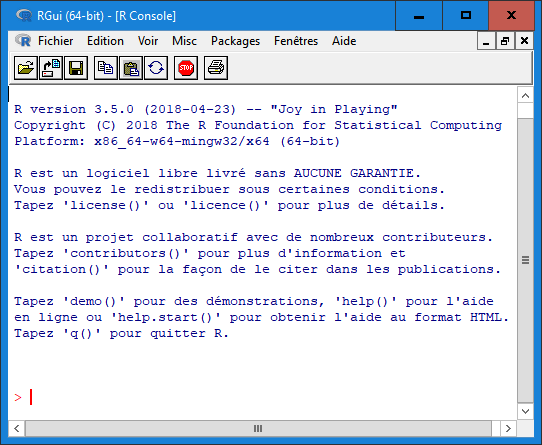
\includegraphics[width=7.53in]{myFigures/screencap_rConsoleFR} \caption{Captura de pantalla de la consola R en Windows.\label{fig:screenCapConsole}}\label{fig:screenCapConsole}
\end{figure}

La consola corresponde a la interfaz donde se interpretará el código, es
decir, donde el código será transformado en lenguaje de máquina,
ejecutado por la computadora y retransmitido en forma legible por
humanos. Esto es análogo a lo que sucede en una calculadora (Figura
\ref{fig:screenCapConsoleCal}). Así es como se usará R más adelante en
esta sección.

A lo largo de este libro, los ejemplos del código R aparecerán sobre un
fondo gris. Se pueden copiar y pegar directamente en la consola, aunque
es mejor reproducir los ejemplos escribiéndolos en la consola (o más
adelante en los scripts) para una mejor comprensión del manejo del
programa R. El resultado de lo que se envía en la consola también
aparecerá en un fondo gris con \texttt{\#\#} delante del código para
hacer la distinción entre el código y el resultado del código.

\begin{figure}
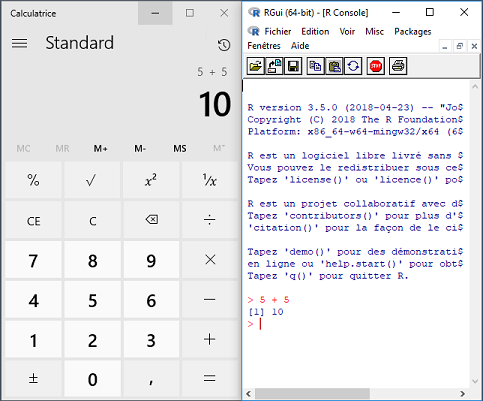
\includegraphics[width=6.71in]{myFigures/screencap_rConsoleCalculatrice} \caption{Captura de pantalla de la consola R al lado de la calculadora de Windows.\label{fig:screenCapConsoleCal}}\label{fig:screenCapConsoleCal}
\end{figure}

\hypertarget{l011opari}{\subsection{Los operadores
aritméticos}\label{l011opari}}

\begin{Shaded}
\begin{Highlighting}[]
\DecValTok{5} \OperatorTok{+}\StringTok{ }\DecValTok{5}
\end{Highlighting}
\end{Shaded}

\begin{verbatim}
## [1] 10
\end{verbatim}

Si escribimos \texttt{5\ +\ 5} en la consola y luego \texttt{Enter}, el
resultado aparece precedido por el número {[}1{]} entre corchetes. Este
número corresponde al número del resultado (en nuestro caso, solo hay un
resultado, volveremos a este aspecto más adelante). También podemos
observar en este ejemplo el uso de espacios antes y después del signo
\texttt{+}. Estos espacios no son necesarios, pero permiten que el
código sea más legible para los humanos (es decir, más agradable de leer
tanto para nosotros como para las personas con las que queremos
compartir nuestro código). Los operadores aritméticos disponibles en R
se resumen en la tabla \ref{tab:tabOpAri}.

\begin{table}

\caption{\label{tab:tabOpAri}Operadores aritméticos.\label{tab:tabOpAri}}
\centering
\begin{tabular}[t]{l|l}
\hline
Label & Operador\\
\hline
adición & +\\
\hline
resta & -\\
\hline
multiplicación & *\\
\hline
división & /\\
\hline
potencia & \textasciicircum{}\\
\hline
módulo & \%\%\\
\hline
cociente decimal & \%/\%\\
\hline
\end{tabular}
\end{table}

Clásicamente, las multiplicaciones y divisiones tienen prioridad sobre
las adiciones y sustracciones. Si es necesario, podemos usar paréntesis.

\begin{Shaded}
\begin{Highlighting}[]
\DecValTok{5} \OperatorTok{+}\StringTok{ }\DecValTok{5} \OperatorTok{*}\StringTok{ }\DecValTok{2}
\end{Highlighting}
\end{Shaded}

\begin{verbatim}
## [1] 15
\end{verbatim}

\begin{Shaded}
\begin{Highlighting}[]
\NormalTok{(}\DecValTok{5} \OperatorTok{+}\StringTok{ }\DecValTok{5}\NormalTok{) }\OperatorTok{*}\StringTok{ }\DecValTok{2}
\end{Highlighting}
\end{Shaded}

\begin{verbatim}
## [1] 20
\end{verbatim}

\begin{Shaded}
\begin{Highlighting}[]
\NormalTok{(}\DecValTok{5} \OperatorTok{+}\StringTok{ }\DecValTok{5}\NormalTok{) }\OperatorTok{*}\StringTok{ }\NormalTok{(}\DecValTok{2} \OperatorTok{+}\StringTok{ }\DecValTok{2}\NormalTok{)}
\end{Highlighting}
\end{Shaded}

\begin{verbatim}
## [1] 40
\end{verbatim}

\begin{Shaded}
\begin{Highlighting}[]
\NormalTok{(}\DecValTok{5} \OperatorTok{+}\StringTok{ }\DecValTok{5}\NormalTok{) }\OperatorTok{*}\StringTok{ }\NormalTok{((}\DecValTok{2} \OperatorTok{+}\StringTok{ }\DecValTok{2}\NormalTok{) }\OperatorTok{/}\StringTok{ }\DecValTok{3}\NormalTok{)}\OperatorTok{^}\DecValTok{2}
\end{Highlighting}
\end{Shaded}

\begin{verbatim}
## [1] 17.77778
\end{verbatim}

El operador \emph{módulo} corresponde al resto de la división
euclidiana. Se usa en ciencias de la computación, por ejemplo, para
saber si un número es par o impar (un número módulo 2 devolverá 1 si es
impar y 0 si es par).

\begin{Shaded}
\begin{Highlighting}[]
\DecValTok{451} \OperatorTok\StringTok{ }\DecValTok{2}
\end{Highlighting}
\end{Shaded}

\begin{verbatim}
## [1] 1
\end{verbatim}

\begin{Shaded}
\begin{Highlighting}[]
\DecValTok{288} \OperatorTok\StringTok{ }\DecValTok{2}
\end{Highlighting}
\end{Shaded}

\begin{verbatim}
## [1] 0
\end{verbatim}

\begin{Shaded}
\begin{Highlighting}[]
\NormalTok{(}\DecValTok{5} \OperatorTok{+}\StringTok{ }\DecValTok{5} \OperatorTok{*}\StringTok{ }\DecValTok{2}\NormalTok{) }\OperatorTok\StringTok{ }\DecValTok{2}
\end{Highlighting}
\end{Shaded}

\begin{verbatim}
## [1] 1
\end{verbatim}

\begin{Shaded}
\begin{Highlighting}[]
\NormalTok{((}\DecValTok{5} \OperatorTok{+}\StringTok{ }\DecValTok{5}\NormalTok{) }\OperatorTok{*}\StringTok{ }\DecValTok{2}\NormalTok{) }\OperatorTok\StringTok{ }\DecValTok{2}
\end{Highlighting}
\end{Shaded}

\begin{verbatim}
## [1] 0
\end{verbatim}

R también incorpora algunas constantes que incluyen \texttt{pi}. Además,
el signo infinito está representado por \texttt{Inf}.

\begin{Shaded}
\begin{Highlighting}[]
\NormalTok{pi}
\end{Highlighting}
\end{Shaded}

\begin{verbatim}
## [1] 3.141593
\end{verbatim}

\begin{Shaded}
\begin{Highlighting}[]
\NormalTok{pi }\OperatorTok{*}\StringTok{ }\DecValTok{5}\OperatorTok{^}\DecValTok{2}
\end{Highlighting}
\end{Shaded}

\begin{verbatim}
## [1] 78.53982
\end{verbatim}

\begin{Shaded}
\begin{Highlighting}[]
\DecValTok{1}\OperatorTok{/}\DecValTok{0}
\end{Highlighting}
\end{Shaded}

\begin{verbatim}
## [1] Inf
\end{verbatim}

El \emph{estilo} del código es importante porque el código está
destinado a ser leído por nosotros y por otras personas. Para tener un
estilo legible, se recomienda colocar espacios antes y después de los
operadores aritméticos, excepto ``*'', ``/'' y ``\^{}'', aunque a veces
es útil agregarlos como es el caso en nuestro ejemplos.

\hypertarget{l011opcomp}{\subsection{Los operadores
comparativos}\label{l011opcomp}}

Sin embargo, R es mucho más que una simple calculadora porque permite
otro tipo de operadores: operadores de comparación, para \emph{comparar}
los valores (Table \ref{tab:tabOpCom}).

\begin{table}

\caption{\label{tab:tabOpCom}Operadores de comparación.\label{tab:tabOpCom}}
\centering
\begin{tabular}[t]{l|l}
\hline
Label & Operador\\
\hline
más pequeño que & <\\
\hline
mayor que & >\\
\hline
más pequeño o igual a & <=\\
\hline
más grande o igual a & >=\\
\hline
igual a & ==\\
\hline
diferente de & !=\\
\hline
\end{tabular}
\end{table}

Por ejemplo, si queremos saber si un numero es más grande que otro,
podemos escribir:

\begin{Shaded}
\begin{Highlighting}[]
\DecValTok{5} \OperatorTok{>}\StringTok{ }\DecValTok{3} 
\end{Highlighting}
\end{Shaded}

\begin{verbatim}
## [1] TRUE
\end{verbatim}

R devuelve \texttt{TRUE} si la comparación es verdadera y \texttt{FALSE}
si la comparación es falsa.

\begin{Shaded}
\begin{Highlighting}[]
\DecValTok{5} \OperatorTok{>}\StringTok{ }\DecValTok{3}
\end{Highlighting}
\end{Shaded}

\begin{verbatim}
## [1] TRUE
\end{verbatim}

\begin{Shaded}
\begin{Highlighting}[]
\DecValTok{2} \OperatorTok{<}\StringTok{ }\FloatTok{1.5}
\end{Highlighting}
\end{Shaded}

\begin{verbatim}
## [1] FALSE
\end{verbatim}

\begin{Shaded}
\begin{Highlighting}[]
\DecValTok{2} \OperatorTok{<=}\StringTok{ }\DecValTok{2}
\end{Highlighting}
\end{Shaded}

\begin{verbatim}
## [1] TRUE
\end{verbatim}

\begin{Shaded}
\begin{Highlighting}[]
\FloatTok{3.2} \OperatorTok{>=}\StringTok{ }\FloatTok{1.5}
\end{Highlighting}
\end{Shaded}

\begin{verbatim}
## [1] TRUE
\end{verbatim}

Podemos combinar operadores aritméticos con operadores de comparación.

\begin{Shaded}
\begin{Highlighting}[]
\NormalTok{(}\DecValTok{5} \OperatorTok{+}\StringTok{ }\DecValTok{8}\NormalTok{) }\OperatorTok{>}\StringTok{ }\NormalTok{(}\DecValTok{3} \OperatorTok{*}\StringTok{ }\DecValTok{45}\OperatorTok{/}\DecValTok{2}\NormalTok{) }
\end{Highlighting}
\end{Shaded}

\begin{verbatim}
## [1] FALSE
\end{verbatim}

En la comparación \texttt{(5\ +\ 8)\ \textgreater{}\ (3\ *\ 45/2)} no se
necesitan paréntesis, pero permiten que el código sea más fácil de leer.

Un operador de comparación particular es \emph{igual a}. Veremos en la
siguiente sección que el signo \texttt{=} está reservado para otro uso:
permite asignar un valor a un objeto. El operador de comparación
\emph{igual a} debe ser diferente, por eso R usa \texttt{==}.

\begin{Shaded}
\begin{Highlighting}[]
\DecValTok{42} \OperatorTok{==}\StringTok{ }\DecValTok{53}
\end{Highlighting}
\end{Shaded}

\begin{verbatim}
## [1] FALSE
\end{verbatim}

\begin{Shaded}
\begin{Highlighting}[]
\DecValTok{58} \OperatorTok{==}\StringTok{ }\DecValTok{58}
\end{Highlighting}
\end{Shaded}

\begin{verbatim}
## [1] TRUE
\end{verbatim}

Otro operador particular es \emph{diferente de}. Se usa con \emph{un
signo de admiración} seguido de \emph{igual}, \texttt{!=}. Este operador
permite obtener la respuesta opuesta a \texttt{==}.

\begin{Shaded}
\begin{Highlighting}[]
\DecValTok{42} \OperatorTok{==}\StringTok{ }\DecValTok{53}
\end{Highlighting}
\end{Shaded}

\begin{verbatim}
## [1] FALSE
\end{verbatim}

\begin{Shaded}
\begin{Highlighting}[]
\DecValTok{42} \OperatorTok{!=}\StringTok{ }\DecValTok{53}
\end{Highlighting}
\end{Shaded}

\begin{verbatim}
## [1] TRUE
\end{verbatim}

\begin{Shaded}
\begin{Highlighting}[]
\NormalTok{(}\DecValTok{3} \OperatorTok{+}\StringTok{ }\DecValTok{2}\NormalTok{) }\OperatorTok{!=}\StringTok{ }\DecValTok{5}
\end{Highlighting}
\end{Shaded}

\begin{verbatim}
## [1] FALSE
\end{verbatim}

\begin{Shaded}
\begin{Highlighting}[]
\DecValTok{10}\OperatorTok{/}\DecValTok{2} \OperatorTok{==}\StringTok{ }\DecValTok{5}
\end{Highlighting}
\end{Shaded}

\begin{verbatim}
## [1] TRUE
\end{verbatim}

R usa \texttt{TRUE} y \texttt{FALSE}, que también son valores que se
pueden probar con operadores de comparación. Pero R también asigna un
valor a \texttt{TRUE} y \texttt{FALSE}:

\begin{Shaded}
\begin{Highlighting}[]
\OtherTok{TRUE} \OperatorTok{==}\StringTok{ }\OtherTok{TRUE}
\end{Highlighting}
\end{Shaded}

\begin{verbatim}
## [1] TRUE
\end{verbatim}

\begin{Shaded}
\begin{Highlighting}[]
\OtherTok{TRUE} \OperatorTok{>}\StringTok{ }\OtherTok{FALSE}
\end{Highlighting}
\end{Shaded}

\begin{verbatim}
## [1] TRUE
\end{verbatim}

\begin{Shaded}
\begin{Highlighting}[]
\DecValTok{1} \OperatorTok{==}\StringTok{ }\OtherTok{TRUE}
\end{Highlighting}
\end{Shaded}

\begin{verbatim}
## [1] TRUE
\end{verbatim}

\begin{Shaded}
\begin{Highlighting}[]
\DecValTok{0} \OperatorTok{==}\StringTok{ }\OtherTok{FALSE}
\end{Highlighting}
\end{Shaded}

\begin{verbatim}
## [1] TRUE
\end{verbatim}

\begin{Shaded}
\begin{Highlighting}[]
\OtherTok{TRUE} \OperatorTok{+}\StringTok{ }\DecValTok{1}
\end{Highlighting}
\end{Shaded}

\begin{verbatim}
## [1] 2
\end{verbatim}

\begin{Shaded}
\begin{Highlighting}[]
\OtherTok{FALSE} \OperatorTok{+}\StringTok{ }\DecValTok{1}
\end{Highlighting}
\end{Shaded}

\begin{verbatim}
## [1] 1
\end{verbatim}

\begin{Shaded}
\begin{Highlighting}[]
\NormalTok{(}\OtherTok{FALSE} \OperatorTok{+}\StringTok{ }\DecValTok{1}\NormalTok{) }\OperatorTok{==}\StringTok{ }\OtherTok{TRUE}
\end{Highlighting}
\end{Shaded}

\begin{verbatim}
## [1] TRUE
\end{verbatim}

El valor de \texttt{TRUE} es 1 y el valor de \texttt{FALSE} es 0.
Veremos más adelante cómo usar esta información en los próximos
capítulos.

R es también un lenguaje relativamente permisivo, significa que admite
cierta flexibilidad en la forma de escribir el código. Debatir sobre la
idoneidad de esta flexibilidad está fuera del alcance de este libro,
pero podemos encontrar en el código R en Internet o en otras obras el
atajo \texttt{T} para \texttt{TRUE} y \texttt{F} for \texttt{FALSE}.

\begin{Shaded}
\begin{Highlighting}[]
\NormalTok{T }\OperatorTok{==}\StringTok{ }\OtherTok{TRUE}
\end{Highlighting}
\end{Shaded}

\begin{verbatim}
## [1] TRUE
\end{verbatim}

\begin{Shaded}
\begin{Highlighting}[]
\NormalTok{F }\OperatorTok{==}\StringTok{ }\OtherTok{FALSE}
\end{Highlighting}
\end{Shaded}

\begin{verbatim}
## [1] TRUE
\end{verbatim}

\begin{Shaded}
\begin{Highlighting}[]
\NormalTok{T }\OperatorTok{==}\StringTok{ }\DecValTok{1}
\end{Highlighting}
\end{Shaded}

\begin{verbatim}
## [1] TRUE
\end{verbatim}

\begin{Shaded}
\begin{Highlighting}[]
\NormalTok{F }\OperatorTok{==}\StringTok{ }\DecValTok{0}
\end{Highlighting}
\end{Shaded}

\begin{verbatim}
## [1] TRUE
\end{verbatim}

\begin{Shaded}
\begin{Highlighting}[]
\NormalTok{(F }\OperatorTok{+}\StringTok{ }\DecValTok{1}\NormalTok{) }\OperatorTok{==}\StringTok{ }\OtherTok{TRUE}
\end{Highlighting}
\end{Shaded}

\begin{verbatim}
## [1] TRUE
\end{verbatim}

Aunque esta forma de referirse a \texttt{TRUE} y \texttt{FALSE} por
\texttt{T} y \texttt{F} está bastante extendida, en este libro siempre
usaremos \texttt{TRUE} y \texttt{FALSE} para que el código sea más fácil
de leer. Como mencionado anterioramente, el objetivo de un código no
solo es ser funcional sino también fácil de leer y volver a leer.

\subsection{Los operadores lógicos}\label{l011oplog}

Hay un último tipo de operador, los operadores lógicos. Estos son útiles
para combinar operadores de comparación (Table \ref{tab:tabOpLog}).

\begin{table}

\caption{\label{tab:tabOpLog}Operadores lógicos.\label{tab:tabOpLog}}
\centering
\begin{tabular}[t]{l|l}
\hline
Label & Operador\\
\hline
no es & !\\
\hline
y & \&\\
\hline
o & |\\
\hline
o exclusivo & xor()\\
\hline
\end{tabular}
\end{table}

\begin{Shaded}
\begin{Highlighting}[]
\OperatorTok{!}\OtherTok{TRUE}
\end{Highlighting}
\end{Shaded}

\begin{verbatim}
## [1] FALSE
\end{verbatim}

\begin{Shaded}
\begin{Highlighting}[]
\OperatorTok{!}\OtherTok{FALSE}
\end{Highlighting}
\end{Shaded}

\begin{verbatim}
## [1] TRUE
\end{verbatim}

\begin{Shaded}
\begin{Highlighting}[]
\NormalTok{((}\DecValTok{3} \OperatorTok{+}\StringTok{ }\DecValTok{2}\NormalTok{) }\OperatorTok{==}\StringTok{ }\DecValTok{5}\NormalTok{) }\OperatorTok{&}\StringTok{ }\NormalTok{((}\DecValTok{3} \OperatorTok{+}\StringTok{ }\DecValTok{3}\NormalTok{) }\OperatorTok{==}\StringTok{ }\DecValTok{5}\NormalTok{)}
\end{Highlighting}
\end{Shaded}

\begin{verbatim}
## [1] FALSE
\end{verbatim}

\begin{Shaded}
\begin{Highlighting}[]
\NormalTok{((}\DecValTok{3} \OperatorTok{+}\StringTok{ }\DecValTok{2}\NormalTok{) }\OperatorTok{==}\StringTok{ }\DecValTok{5}\NormalTok{) }\OperatorTok{&}\StringTok{ }\NormalTok{((}\DecValTok{3} \OperatorTok{+}\StringTok{ }\DecValTok{3}\NormalTok{) }\OperatorTok{==}\StringTok{ }\DecValTok{6}\NormalTok{)}
\end{Highlighting}
\end{Shaded}

\begin{verbatim}
## [1] TRUE
\end{verbatim}

\begin{Shaded}
\begin{Highlighting}[]
\NormalTok{(}\DecValTok{3} \OperatorTok{<}\StringTok{ }\DecValTok{5}\NormalTok{) }\OperatorTok{&}\StringTok{ }\NormalTok{(}\DecValTok{5} \OperatorTok{<}\StringTok{ }\DecValTok{5}\NormalTok{)}
\end{Highlighting}
\end{Shaded}

\begin{verbatim}
## [1] FALSE
\end{verbatim}

\begin{Shaded}
\begin{Highlighting}[]
\NormalTok{(}\DecValTok{3} \OperatorTok{<}\StringTok{ }\DecValTok{5}\NormalTok{) }\OperatorTok{&}\StringTok{ }\NormalTok{(}\DecValTok{5} \OperatorTok{<=}\StringTok{ }\DecValTok{5}\NormalTok{)}
\end{Highlighting}
\end{Shaded}

\begin{verbatim}
## [1] TRUE
\end{verbatim}

El operador lógico \texttt{xor()} es \emph{o exclusivo}. Es decir, uno
de los dos \textbf{argumentos} de la \textbf{función} \texttt{xor()}
debe ser verdadero, pero no ambos. Más adelante volveremos a las
\textbf{funciones} y sus \textbf{argumentos}, pero recuerde que
identificamos una función por sus paréntesis que contienen argumentos
separados por comas.

\begin{Shaded}
\begin{Highlighting}[]
\KeywordTok{xor}\NormalTok{((}\DecValTok{3} \OperatorTok{+}\StringTok{ }\DecValTok{2}\NormalTok{) }\OperatorTok{==}\StringTok{ }\DecValTok{5}\NormalTok{, (}\DecValTok{3} \OperatorTok{+}\StringTok{ }\DecValTok{3}\NormalTok{) }\OperatorTok{==}\StringTok{ }\DecValTok{6}\NormalTok{)}
\end{Highlighting}
\end{Shaded}

\begin{verbatim}
## [1] FALSE
\end{verbatim}

\begin{Shaded}
\begin{Highlighting}[]
\KeywordTok{xor}\NormalTok{((}\DecValTok{3} \OperatorTok{+}\StringTok{ }\DecValTok{2}\NormalTok{) }\OperatorTok{==}\StringTok{ }\DecValTok{5}\NormalTok{, (}\DecValTok{3} \OperatorTok{+}\StringTok{ }\DecValTok{2}\NormalTok{) }\OperatorTok{==}\StringTok{ }\DecValTok{6}\NormalTok{)}
\end{Highlighting}
\end{Shaded}

\begin{verbatim}
## [1] TRUE
\end{verbatim}

\begin{Shaded}
\begin{Highlighting}[]
\KeywordTok{xor}\NormalTok{((}\DecValTok{3} \OperatorTok{+}\StringTok{ }\DecValTok{3}\NormalTok{) }\OperatorTok{==}\StringTok{ }\DecValTok{5}\NormalTok{, (}\DecValTok{3} \OperatorTok{+}\StringTok{ }\DecValTok{2}\NormalTok{) }\OperatorTok{==}\StringTok{ }\DecValTok{6}\NormalTok{)}
\end{Highlighting}
\end{Shaded}

\begin{verbatim}
## [1] FALSE
\end{verbatim}

\begin{Shaded}
\begin{Highlighting}[]
\KeywordTok{xor}\NormalTok{((}\DecValTok{3} \OperatorTok{+}\StringTok{ }\DecValTok{3}\NormalTok{) }\OperatorTok{==}\StringTok{ }\DecValTok{5}\NormalTok{, (}\DecValTok{3} \OperatorTok{+}\StringTok{ }\DecValTok{3}\NormalTok{) }\OperatorTok{==}\StringTok{ }\DecValTok{6}\NormalTok{)}
\end{Highlighting}
\end{Shaded}

\begin{verbatim}
## [1] TRUE
\end{verbatim}

Se recomienda que las comas \texttt{,} sean seguidas de un espacio para
que el código sea más agradable de leer.

\subsection{Ayuda a los operadores}\label{ayuda-a-los-operadores}

El archivo de ayuda en inglés sobre operadores aritméticos se puede
obtener con el comando \texttt{?\textquotesingle{}+\textquotesingle{}}.
El de los operadores de comparación con el comando
\texttt{?\textquotesingle{}==\textquotesingle{}} y el de los operadores
lógicos con el comando \texttt{?\textquotesingle{}\&\textquotesingle{}}.

\hypertarget{l011object}{\section{El concepto de
objeto}\label{l011object}}

Un aspecto importante de la programación con R, pero también la
programación en general es la noción de objeto. Como se indica en la
página web de wikipedia
(\url{https://ia.wikipedia.org/wiki/Objecto_(informatica)}), en ciencias
de la computación, un objeto es un \emph{contenedor}, es decir, algo que
contendrá información. La información contenida en un objeto puede ser
muy diversa, pero por el momento contendremos en un objeto el número 5.
Para hacer esto (y para reutilizarlo más adelante), debemos darle un
nombre a nuestro objeto. En R, los nombres de los objetos no deben
contener caracteres especiales como \emph{\^{} \$ ? \textbar{} + ()
{[}{]} \{\}}, entre otros. No deben comenzar con un número ni contener
espacios. El nombre del objeto debe ser representativo de lo que
contiene, sin ser demasiado corto ni demasiado largo. Imagine que
nuestro número 5 corresponde al número de repeticiones de un
experimento. Nos gustaría darle un nombre que se refiera a \emph{numero}
y \emph{repeticiones}, que podríamos reducir a \emph{nbr} y \emph{rep},
respectivamente (\emph{nbr} para number en ingles). Hay varias
posibilidades que son bastante comunes bajo R:

\begin{itemize}
\tightlist
\item
  la separación mediante \emph{guión bajo} (underscore):
  \texttt{nbr\_rep}
\item
  la separación mediante el carácter \emph{punto}: \texttt{nbr.rep}
\item
  el uso de letras minúsculas: \texttt{nbrrep}
\item
  el estilo \emph{lowerCamelCase} que consiste en una primera palabra en
  minúscula y la primera letra de las siguientes palabras con una letra
  mayúscula: \texttt{nbrRep}
\item
  el estilo \emph{UpperCamelCase} donde cada palabra comienza con una
  letra mayúscula: \texttt{NbrRep}
\end{itemize}

Todas estas formas de nombrar un objeto son equivalentes. En este libro
usaremos el estilo \emph{lowerCamelCase}. En general, debemos evitar los
nombres que son demasiado largos, como
\texttt{miNumeroDeRepeticionesDeMiExperimento} o demasiado cortos como
\texttt{nR}, y los nombres que no permiten identificar los contenidos
como \texttt{miVariable} o \texttt{miNumero}, asi que nombres como
\texttt{a} o \texttt{b}. El objetivo es de tener una idea de lo que hay
en cada objeto en base a su nombre.

Hay diferentes maneras de definir un nombre para los objetos que
crearemos con R. En este libro, utilizamos el estilo
\emph{lowerCamelCase}. Lo importante no es la elección del estilo, sino
la consistencia en su elección. El objetivo es tener un código
funcional, pero también un código que sea fácil y agradable de leer para
nosotros y para los demás.

Ahora que hemos elegido un nombre para nuestro objeto, debemos crearlo y
hacer que R entienda que nuestro objeto debe contener el número 5. Hay
tres maneras de crear un objeto bajo R:

\begin{itemize}
\tightlist
\item
  con \texttt{\textless{}-}
\item
  con \texttt{=}
\item
  o con \texttt{-\textgreater{}}
\end{itemize}

\begin{Shaded}
\begin{Highlighting}[]
\NormalTok{nbrRep <-}\StringTok{ }\DecValTok{5}
\NormalTok{nbrRep =}\StringTok{ }\DecValTok{5}
\DecValTok{5}\NormalTok{ ->}\StringTok{ }\NormalTok{nbrRep}
\end{Highlighting}
\end{Shaded}

En este libro siempre usaremos la forma \texttt{\textless{}-} para
coherencia y también porque es la forma más común.

\begin{Shaded}
\begin{Highlighting}[]
\NormalTok{nbrRep <-}\StringTok{ }\DecValTok{5}
\end{Highlighting}
\end{Shaded}

Acabamos de crear un objeto \texttt{nbrRep} y establecerlo con el valor
\emph{5}. Este objeto ahora está disponible en nuestro entorno de
computación y puede ser utilizado. Algunos ejemplos :

\begin{Shaded}
\begin{Highlighting}[]
\NormalTok{nbrRep }\OperatorTok{+}\StringTok{ }\DecValTok{2}
\end{Highlighting}
\end{Shaded}

\begin{verbatim}
## [1] 7
\end{verbatim}

\begin{Shaded}
\begin{Highlighting}[]
\NormalTok{nbrRep }\OperatorTok{*}\StringTok{ }\DecValTok{5} \OperatorTok{-}\StringTok{ }\DecValTok{45}\OperatorTok{/}\DecValTok{56}
\end{Highlighting}
\end{Shaded}

\begin{verbatim}
## [1] 24.19643
\end{verbatim}

\begin{Shaded}
\begin{Highlighting}[]
\NormalTok{pi }\OperatorTok{*}\StringTok{ }\NormalTok{nbrRep}\OperatorTok{^}\DecValTok{2}
\end{Highlighting}
\end{Shaded}

\begin{verbatim}
## [1] 78.53982
\end{verbatim}

El valor asociado con nuestro objeto \texttt{nbrRep} se puede modificar
de la misma manera que cuando se creó:

\begin{Shaded}
\begin{Highlighting}[]
\NormalTok{nbrRep <-}\StringTok{ }\DecValTok{5}
\NormalTok{nbrRep }\OperatorTok{+}\StringTok{ }\DecValTok{2}
\end{Highlighting}
\end{Shaded}

\begin{verbatim}
## [1] 7
\end{verbatim}

\begin{Shaded}
\begin{Highlighting}[]
\NormalTok{nbrRep <-}\StringTok{ }\DecValTok{10}
\NormalTok{nbrRep }\OperatorTok{+}\StringTok{ }\DecValTok{2}
\end{Highlighting}
\end{Shaded}

\begin{verbatim}
## [1] 12
\end{verbatim}

\begin{Shaded}
\begin{Highlighting}[]
\NormalTok{nbrRep <-}\StringTok{ }\DecValTok{5} \OperatorTok{*}\StringTok{ }\DecValTok{2} \OperatorTok{+}\StringTok{ }\DecValTok{7}\OperatorTok{/}\DecValTok{3}
\NormalTok{nbrRep }\OperatorTok{+}\StringTok{ }\DecValTok{2}
\end{Highlighting}
\end{Shaded}

\begin{verbatim}
## [1] 14.33333
\end{verbatim}

El uso de objetos tiene sentido cuando tenemos operaciones complejas
para realizar y hace que el código sea más agradable de leer y entender.

\begin{Shaded}
\begin{Highlighting}[]
\NormalTok{(}\DecValTok{5} \OperatorTok{+}\StringTok{ }\DecValTok{9}\OperatorTok{^}\DecValTok{2} \OperatorTok{-}\StringTok{ }\DecValTok{1}\OperatorTok{/}\DecValTok{18}\NormalTok{) }\OperatorTok{/}\StringTok{ }\NormalTok{(}\DecValTok{32} \OperatorTok{*}\StringTok{ }\DecValTok{45}\OperatorTok{/}\DecValTok{8} \OperatorTok{+}\StringTok{ }\DecValTok{3}\NormalTok{)}
\end{Highlighting}
\end{Shaded}

\begin{verbatim}
## [1] 0.4696418
\end{verbatim}

\begin{Shaded}
\begin{Highlighting}[]
\NormalTok{termino01 <-}\StringTok{ }\DecValTok{5} \OperatorTok{+}\StringTok{ }\DecValTok{9}\OperatorTok{^}\DecValTok{2} \OperatorTok{-}\StringTok{ }\DecValTok{1}\OperatorTok{/}\DecValTok{18}
\NormalTok{termino02 <-}\StringTok{ }\DecValTok{32} \OperatorTok{*}\StringTok{ }\DecValTok{45}\OperatorTok{/}\DecValTok{8} \OperatorTok{+}\StringTok{ }\DecValTok{3}
\NormalTok{termino01 }\OperatorTok{/}\StringTok{ }\NormalTok{termino02}
\end{Highlighting}
\end{Shaded}

\begin{verbatim}
## [1] 0.4696418
\end{verbatim}

\section{Los scripts}\label{los-scripts}

R es un lenguaje de programación denominado \emph{lenguaje de
scripting}. Esto se refiere al hecho de que la mayoría de los usuarios
escribirán pequeñas piezas de código en lugar de programas completos. R
se puede usar como una simple calculadora, y en este caso no será
necesario mantener un historial de las operaciones que se han realizado.
Pero si las operaciones a implementar son largas y complejas, puede ser
necesario e interesante guardar lo que se ha hecho para poder continuar
más adelante. El archivo en el que se almacenarán las operaciones es lo
que comúnmente se llama el \emph{script}. Un \emph{script}, por lo
tanto, es un archivo que contiene una sucesión de información
comprensible por R y que es posible ejecutar.

\subsection{Crear un script y
documentarlo}\label{crear-un-script-y-documentarlo}

Para crear un nuevo script basta con abrir un documento vacío de texto,
que será editado por un editor de texto como el bloc de notas en Windows
o Mac OSX, o Gedit o incluso nano en Linux. Por convención, este archivo
toma la extensión ``.r'' o ``.R'' (lo mas comun). Esta última convención
se usará en este libro (\emph{``miArchivo.R''}). Desde la interfaz
gráfica de R, es posible crear un nuevo script en Mac OS y Windows a
través de \emph{file}, luego \emph{new script} y \emph{save as}. Al
igual que el nombre de los objetos, el nombre del script es importante
para que podamos identificar fácilmente su contenido. Por ejemplo,
podríamos crear un archivo \texttt{formRConceptsBase.R} que contenga los
objetos que acabamos de crear y los cálculos que hicimos. Pero incluso
con nombres de objetos y archivos bien definidos, será difícil recordar
el significado de este archivo sin la documentación que acompaña a este
script. Para documentar un script utilizaremos \emph{comentarios}. Los
\emph{comentarios} son elementos que R identificará como tales y no se
ejecutarán. Para especificar a R que vamos a hacer un \emph{comentario},
debemos usar el carácter octothorpe (corsé o numeral) \texttt{\#}. Los
comentarios se pueden insertar en una nueva línea o al final de la
línea.

\begin{Shaded}
\begin{Highlighting}[]
\CommentTok{# creación objeto número de repeticiones}
\NormalTok{nbrRep <-}\StringTok{ }\DecValTok{5} \CommentTok{# Comentario de fin de línea}
\end{Highlighting}
\end{Shaded}

Todo lo que hay despues del simbolo numeral \texttt{\#} no sera
ejecutado. Significa que podriamos usar comentarios como \texttt{\#\#\#}
o \texttt{\#comentario}, aun que se recomienda hacer comentarios con un
solo simbolo numeral seguido por un espacio y despues su comentario:
\texttt{\#\ mi\ comentario}.

Los comentarios también se pueden usar para hacer que una línea ya no se
ejecute. En este caso no queremos ejecutar la secunda linea:

\begin{Shaded}
\begin{Highlighting}[]
\NormalTok{nbrRep <-}\StringTok{ }\DecValTok{5}
\CommentTok{# nbrRep + 5}
\end{Highlighting}
\end{Shaded}

Para volver a la documentación del script, se recomienda comenzar cada
uno de nuestros scripts con una breve descripción de su contenido, luego
cuando el script sea extenso, estructurarlo en diferentes partes para
facilitar su lectura.

\begin{Shaded}
\begin{Highlighting}[]
\CommentTok{# ------------------------------------------------------------}
\CommentTok{# Aquí hay un script para adquirir los conceptos básicos}
\CommentTok{# con R}
\CommentTok{# fecha de creación : 27/06/2018}
\CommentTok{# autor : François Rebaudo}
\CommentTok{# ------------------------------------------------------------}

\CommentTok{# [1] creación del objeto número de repeticiones}
\CommentTok{# ------------------------------------------------------------}

\NormalTok{nbrRep <-}\StringTok{ }\DecValTok{5}

\CommentTok{# [2] cálculos simples}
\CommentTok{# ------------------------------------------------------------}

\NormalTok{pi }\OperatorTok{*}\StringTok{ }\NormalTok{nbrRep}\OperatorTok{^}\DecValTok{2}
\end{Highlighting}
\end{Shaded}

\begin{verbatim}
## [1] 78.53982
\end{verbatim}

Para ir más allá en el estilo del código, una guía completa de
recomendaciones está disponible en línea en el sitio web
\emph{tidyverse} (en ingles ; \url{http://style.tidyverse.org/}).

\subsection{Ejecutar un script}\label{ejecutar-un-script}

Como tenemos un script, no trabajamos directamente en la consola. Pero
solo la consola puede \emph{entender} el código R y devolvernos los
resultados que queremos obtener. Por ahora, la técnica más simple es
copiar y pegar las líneas que queremos ejecutar desde nuestro script
hasta la consola. A partir de ahora, ya no utilizaremos editores de
texto como bloc de notas, sino editores especializados para la creación
de scripts R. Sera es el objetivo del siguiente capítulo.

\section{Conclusión}\label{conclusion}

Felicitaciones, hemos llegado al final de este primer capítulo sobre la
base de R. Sabemos:

\begin{itemize}
\tightlist
\item
  Instalar R
\item
  Usar R como una calculadora
\item
  Crear \textbf{objetos} y utilisarlos para los calculos aritméticos,
  comparativos y logicos
\item
  Elejir nombres pertinentes para los objetos
\item
  Crear un nuevo \textbf{script}
\item
  Elejir un nombre pertinente para el archivo del script
\item
  Ejecutar el codigo de un script
\item
  Documentar los scripts con \textbf{comentarios}
\item
  Usar un estilo de código para que sea agradable de leer y facil de
  entender
\end{itemize}

\hypertarget{IDE}{\chapter{Elegir un entorno de desarrollo}\label{IDE}}

\section{Editores de texto y entorno de
desarrollo}\label{editores-de-texto-y-entorno-de-desarrollo}

Hay muchos editores de texto, el capítulo anterior permitió introducir
algunos de los más simples como el bloc de notas de Windows. Sin
embargo, los límites de estos editores han hecho tediosa la tarea de
escribir un script. De hecho, incluso estructurando su script con
comentarios, sigue siendo difícil entenderlo. Aquí es donde entran los
editores de texto especializados para facilitar la escritura y la
lectura de scripts. El editor de texto para R más común es Rstudio, pero
hay muchos más. Hacer una lista exhaustiva de todas las soluciones
disponibles está más allá del alcance de este libro, por lo que nos
centraremos en las tres soluciones que utilizo a diario:
\textbf{Notepad++}, \textbf{Rstudio} y \textbf{Geany}. No necesita
instalar más de un editor de texto. Aquí recomendamos RStudio para
principiantes a R.

\section{RStudio}\label{rstudio}

\begin{figure}

\includegraphics[width=7.78in]{myLogos/RStudio} \caption{Logo RStudio.\label{fig:logoRStudio}}\label{fig:logoRStudio}
\end{figure}

\subsection{Instalar RStudio}\label{instalar-rstudio}

El programa para instalar el software RStudio se encuentra en la parte
\emph{Products} del sitio web de RStudio
(\url{https://www.rstudio.com/}). Instalaremos RStudio para uso local
(en nuestra computadora), por lo que la versión que nos interesa es
\emph{Desktop}. Usaremos la versión \emph{Open Source} que es gratuita.
Luego, seleccionamos la versión que corresponde a nuestro sistema
operativo (Windows, Mac OS, Linux), descargamos el archivo
correspondiente y lo ejecutamos para comenzar la instalación. Podemos
mantener las opciones predeterminadas durante la instalación.

\subsection{Un script con RStudio}\label{un-script-con-rstudio}

Podemos abrir RStudio. En la primera apertura, la interfaz se divide en
dos con la consola R a la izquierda que vimos en el capítulo anterior
(Figura \ref{fig:screenCapRStudio01}). Para abrir un nuevo script, vamos
al menú \emph{Archivo} (o \emph{File}), \emph{Nuevo archivo} (o
\emph{New File}), \emph{R script}. Por defecto, este archivo tiene el
nombre \emph{Untitled1}. Hemos visto en el capítulo anterior la
importancia de dar un nombre pertinente a nuestros scripts, por lo que
lo cambiaremos de nombre a \emph{selecEnvDev.R}, en el menú
\emph{Archivo} (o \emph{File}), con la opción \emph{Guardar como
\ldots{}} (o \emph{Save As\ldots{}}). Podemos notar que el lado
izquierdo de RStudio ahora está dividido en dos, con la consola en la
parte inferior de la pantalla y el script en la parte superior.

\begin{figure}
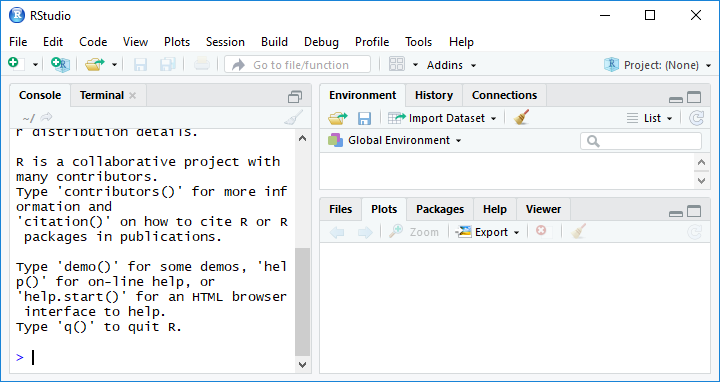
\includegraphics[width=10in]{myFigures/screencap_RStudio_01} \caption{Captura de pantalla de RStudio en Windows: pantalla por defecto.\label{fig:screenCapRStudio01}}\label{fig:screenCapRStudio01}
\end{figure}

Luego podemos comenzar a escribir nuestro script con los comentarios que
describan lo que vamos a encontrar allí, y agregar un cálculo simple.
Una vez que hayamos copiado o escrito un código, podemos guardar nuestro
script con el comando \texttt{CTRL\ +\ S} o yendo a \emph{Archivo} (o
\emph{File}, luego \emph{Guardar} (o \emph{Save}).

\begin{Shaded}
\begin{Highlighting}[]
\CommentTok{# ------------------------------------------------------------}
\CommentTok{# Un script para seleccionar su entorno de desarrollo}
\CommentTok{# fecha de creación : 27/06/2018}
\CommentTok{# autor : François Rebaudo}
\CommentTok{# ------------------------------------------------------------}

\CommentTok{# [1] cálculos simples}
\CommentTok{# ------------------------------------------------------------}
\NormalTok{nbrRep <-}\StringTok{ }\DecValTok{5}
\NormalTok{pi }\OperatorTok{*}\StringTok{ }\NormalTok{nbrRep}\OperatorTok{^}\DecValTok{2}
\end{Highlighting}
\end{Shaded}

\begin{verbatim}
## [1] 78.53982
\end{verbatim}

Para ejecutar nuestro script, simplemente seleccionamos las líneas que
deseamos ejecutar y usamos la combinación de teclas
\texttt{CTRL\ +\ ENTER}. El resultado aparece en la consola (Figura
\ref{fig:screenCapRStudio02}).

\begin{figure}
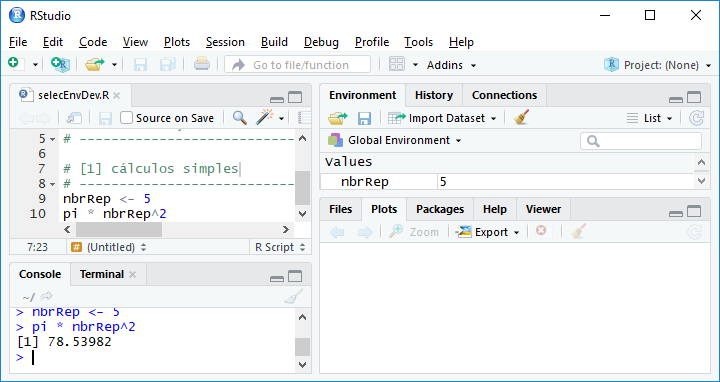
\includegraphics[width=10in]{myFigures/screencap_RStudio_02} \caption{Captura de pantalla de RStudio en Windows: ejecutar nuestro script con CTRL + ENTER.\label{fig:screenCapRStudio02}}\label{fig:screenCapRStudio02}
\end{figure}

Podemos ver que, de forma predeterminada, en la parte del script, los
comentarios aparecen en verde, los números en azul y el resto del código
en negro. En la parte de la consola, lo que se ejecutó aparece en azul y
los resultados de la ejecución en negro. También podemos observar que en
la parte del código cada línea tiene un número correspondiente al número
de línea a la izquierda sobre un fondo gris. Este es el resaltado de
preferencias de sintaxis predeterminado con RStudio. Estas preferencias
de sintaxis pueden modificarse yendo al menú \emph{Herramientas} (o
\emph{Tools}), \emph{Opciones globales \ldots{}} (o \emph{Global
Options\ldots{}}), \emph{Aspecto} (o \emph{Appearance}), y luego
seleccionando otro tema del \emph{Editor de tema:} (o \emph{Editor
theme:}). Elegiremos el tema \emph{Cobalt}, luego \emph{OK} (Figura
\ref{fig:screenCapRStudio03}).

\begin{figure}
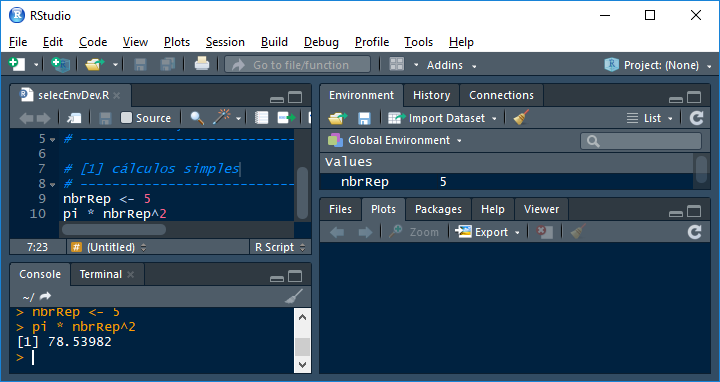
\includegraphics[width=10in]{myFigures/screencap_RStudio_03} \caption{Captura de pantalla de RStudio en Windows: cambiar preferencias de sintaxis.\label{fig:screenCapRStudio03}}\label{fig:screenCapRStudio03}
\end{figure}

Sabemos cómo crear un nuevo script, guardarlo, ejecutar su contenido y
cambiar la apariencia de RStudio. Veremos los muchos otros beneficios de
RStudio a lo largo de este libro, ya que es el entorno de desarrollo que
se utilizará. Sin embargo, seremos especialmente cuidadosos de que todos
los scripts desarrollados a lo largo de este libro se ejecuten de la
misma manera, independientemente del entorno de desarrollo utilizado.

\section{Notepad++ avec Npp2R}\label{notepad-avec-npp2r}

\begin{figure}

\includegraphics[width=7.78in]{myLogos/Notepadpp} \caption{Logo Notepad++\label{fig:logoNotepad}}\label{fig:logoNotepad}
\end{figure}

\subsection{Instalar Notepad++ (solamente para
Windows)}\label{instalar-notepad-solamente-para-windows}

El programa para instalar Notepad ++ se puede encontrar en la pestaña
\emph{Downloads} (\url{https://notepad-plus-plus.org/download/}).
Podemos elegir entre la versión de 32-bit y la de 64-bit (64-bit si no
sabe qué versión elegir). Notepad++ es suficiente para escribir un
script, pero es aún más poderoso con \emph{Notepad++ to R}
(\emph{Npp2R}) que permite ejecutar automáticamente nuestros scripts en
una consola localmente en nuestra computadora o remotamente en un
servidor.

\subsection{Instalar Npp2R}\label{instalar-npp2r}

El programa para instalar Npp2R está alojado en el sitio de Sourceforge
(\url{https://sourceforge.net/projects/npptor/}). Npp2R debe instalarse
después de Notepad++.

\subsection{Un script con Notepad++}\label{un-script-con-notepad}

Al abrir por primera vez, Notepad++ muestra un archivo vacío \emph{new
1} (Figura \ref{fig:screenCapNpp01}).

\begin{figure}
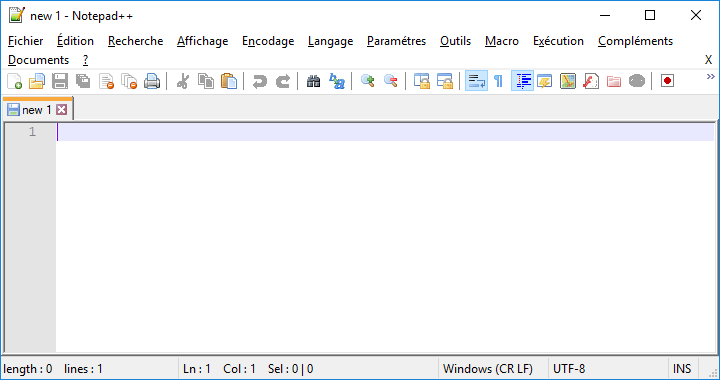
\includegraphics[width=10in]{myFigures/screencap_Npp_01} \caption{Captura de pantalla de Notepad++ en Windows: pantalla por defecto.\label{fig:screenCapNpp01}}\label{fig:screenCapNpp01}
\end{figure}

Como ya hemos creado un script para probarlo con RStudio, lo abriremos
de nuevo con Notepad++. En \emph{Archivo}, seleccionamos \emph{Abrir
\ldots{}} luego elijemos el script \emph{selecEnvDev.R} creado
previamente. Una vez que el script está abierto, vamos a \emph{Idioma},
luego \emph{R}, y de nuevo \emph{R}. Aparece el resaltado de sintaxis
(Figura \ref{fig:screenCapNpp02}).

\begin{figure}
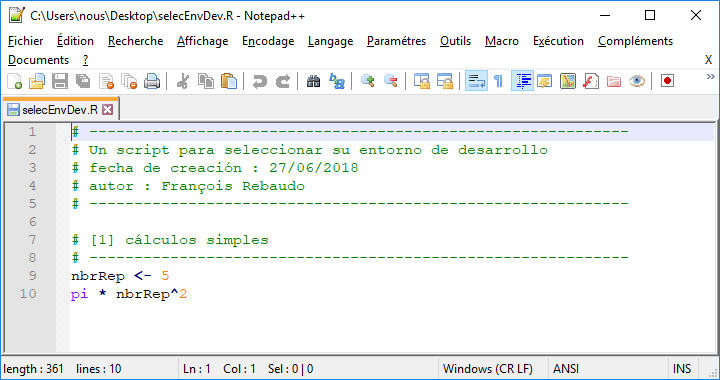
\includegraphics[width=10in]{myFigures/screencap_Npp_02} \caption{Captura de pantalla de Notepad++ en Windows: ejecutar nuestro script con F8.\label{fig:screenCapNpp02}}\label{fig:screenCapNpp02}
\end{figure}

La ejecución del script solo se puede realizar si se está ejecutando
Npp2R. Para hacerlo, es necesario ejecutar el programa Npp2R desde el
prompt de Windows. Un icono debe aparecer en la parte inferior de su
pantalla demostrando que Npp2R está prendido. La ejecución automática
del código de Notepad++ se realiza seleccionando el código para ejecutar
y luego usando el comando \texttt{F8}. Si el comando no funciona, puede
ser necesario reiniciar la computadora. Si el comando funciona, se
abrirá una nueva ventana con una consola que ejecuta las líneas deseadas
(Figura \ref{fig:screenCapNpp03}).

\begin{figure}
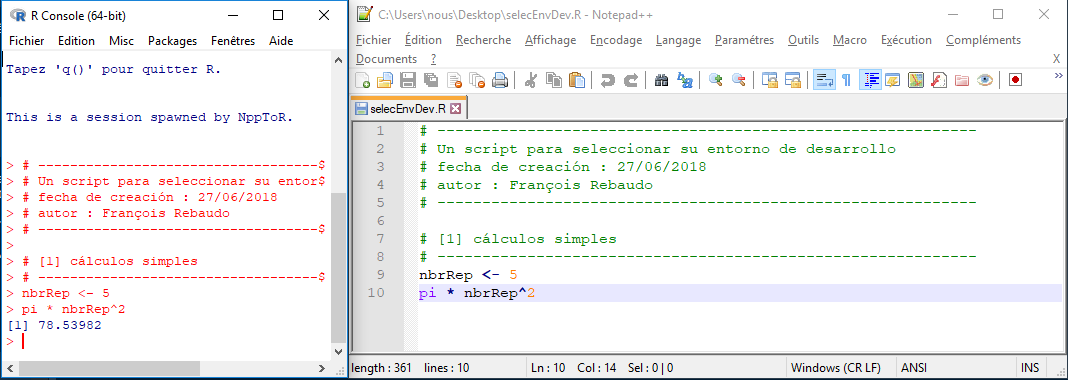
\includegraphics[width=14.83in]{myFigures/screencap_Npp_03} \caption{Captura de pantalla de Notepad++ en Windows: la consola con F8.\label{fig:screenCapNpp03}}\label{fig:screenCapNpp03}
\end{figure}

Al igual que con RStudio, el resaltado de sintaxis se puede cambiar
desde el menú \emph{Configuración}, y se puede seleccionar un nuevo tema
(por ejemplo, \emph{Solarized} en la Figura \ref{fig:screenCapNpp04})

\begin{figure}
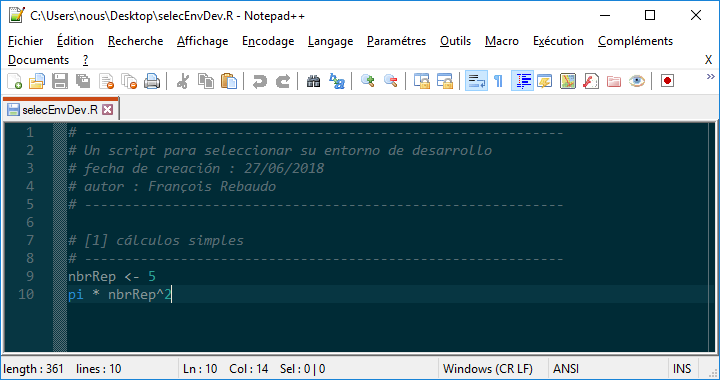
\includegraphics[width=10in]{myFigures/screencap_Npp_04} \caption{Captura de pantalla de Notepad++ en Windows con el tema Solarized.\label{fig:screenCapNpp04}}\label{fig:screenCapNpp04}
\end{figure}

Comparado con otros editores de texto, Notepad++ tiene la ventaja de ser
muy liviano, rapido y ofrece una amplia gama de opciones para
personalizar la escritura de códigos.

\section{Geany}\label{geany}

\begin{figure}

\includegraphics[width=7.78in]{myLogos/Geany} \caption{Logo Geany\label{fig:logoGeany}}\label{fig:logoGeany}
\end{figure}

\subsection{Instalar Geany (para Linux, Mac OSX y
Windows)}\label{instalar-geany-para-linux-mac-osx-y-windows}

El programa para instalar Geany se puede encontrar en la pestaña
\emph{Downloads} en el menú de la izquierda \emph{Releases} de la página
web (\url{https://www.geany.org/}). Luego solo descargamos el ejecutable
para Windows o el dmg para Mac OSX. Los usuarios de Linux preferirán un
\texttt{sudo\ apt-get\ install\ geany}.

\subsection{Un script con Geany}\label{un-script-con-geany}

Al abrir por primera vez, como para RStudio y Notepad++, se crea un
archivo vacío (Figura \ref{fig:screenCapGeany01}).

\begin{figure}
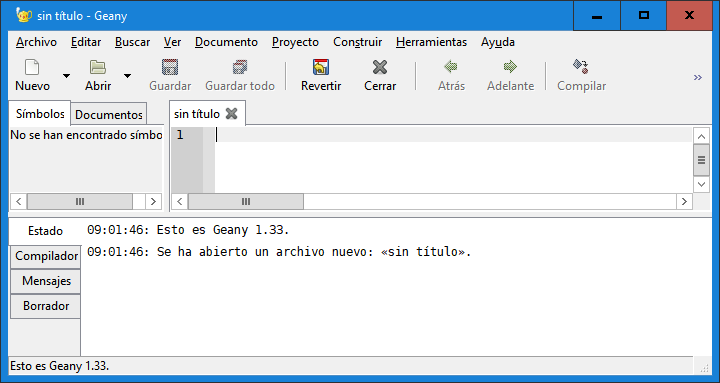
\includegraphics[width=10in]{myFigures/screencap_Geany_01} \caption{Captura de pantalla de Geany en Windows: pantalla por defecto.\label{fig:screenCapGeany01}}\label{fig:screenCapGeany01}
\end{figure}

Podemos abrir nuestro script con \emph{Archivo}, \emph{Abrir} (Figura
\ref{fig:screenCapGeany02}).

\begin{figure}
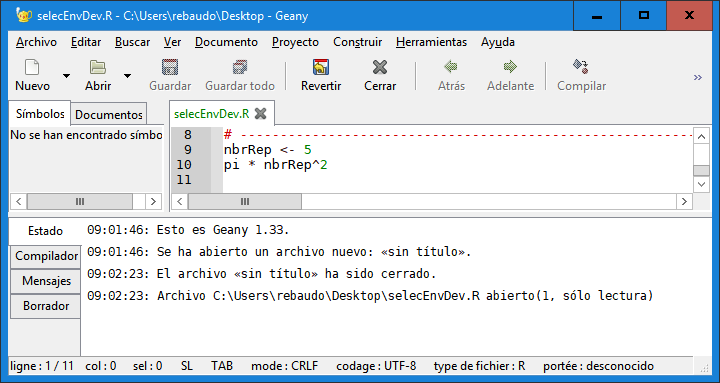
\includegraphics[width=10in]{myFigures/screencap_Geany_02} \caption{Captura de pantalla de Geany en Windows: abrir un script.\label{fig:screenCapGeany02}}\label{fig:screenCapGeany02}
\end{figure}

Para ejecutar nuestro script, la versión de Geany para Windows no tiene
un terminal incorporado, lo que hace que su uso sea limitado bajo este
sistema operativo. La ejecución de un script se puede hacer abriendo R
en una ventana separada y copiando y pegando las líneas que se
ejecutarán. En Linux y Mac OSX, podemos abrir R en el terminal en la
parte inferior de la ventana de Geany con el comando \texttt{R}. Podemos
configurar Geany para una combinación de teclas para ejecutar el código
seleccionado (por ejemplo \texttt{CTRL\ +\ R}). Para esto hay que
permitir el envío de selección al terminal
(\texttt{send\_selection\_unsafe\ =\ true}) in
\texttt{archivo\ geany.conf} y elegir el comando para enviar al terminal
(en \emph{Editar}, \emph{Preferencias}, \emph{Combinaciones}). Para
cambiar el tema de Geany, hay una colección de temas disponibles en
GitHub (\url{https://github.com/geany/geany-themes/}). El tema se puede
cambiar a través del menú \emph{Ver}, \emph{cambiar Esquema del color
\ldots{}} (un ejemplo con el tema \emph{Solarized} Figura @ref(Fig:
screenCapGeany03)).

\begin{figure}
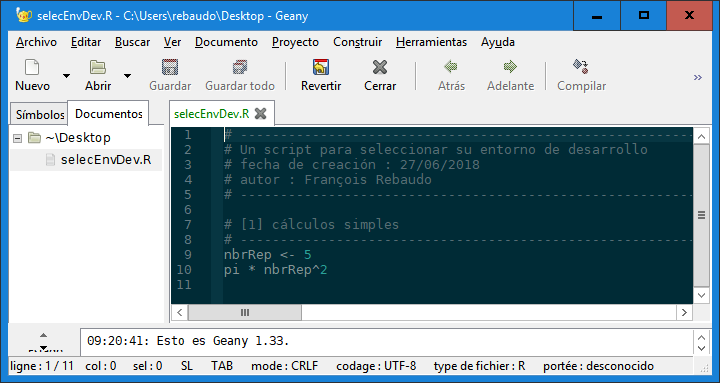
\includegraphics[width=10in]{myFigures/screencap_Geany_03} \caption{Captura de pantalla de Geany en Windows: cambiar esquema de color.\label{fig:screenCapGeany03}}\label{fig:screenCapGeany03}
\end{figure}

\section{Otras soluciones}\label{otras-soluciones}

Hay muchas otras soluciones, algunas especializadas para R como
\textbf{Tinn-R} (\url{https://sourceforge.net/projects/tinn-r/}), y
otras más generales para programación como \textbf{Atom}
(\url{https://atom.io/}), \textbf{Sublime Text}
(\url{https://www.sublimetext.com/}), \textbf{Vim}
(\url{https://www.vim.org/}), \textbf{Gedit}
(\url{https://wiki.gnome.org/Apps/Gedit}), \textbf{GNU Emacs}
(\url{https://www.gnu.org/software/emacs/}), \textbf{Jupyter}
(\url{http://jupyter.org}), o \textbf{Brackets}
(\url{http://brackets.io/}) y \textbf{Eclipse}
(\url{http://www.eclipse.org/}).

\section{Conclusión}\label{conclusion-1}

Felicitaciones, llegamos al final de este capítulo sobre el entorno de
desarrollo para el uso de R. Hasta ahora sabemos:

\begin{itemize}
\tightlist
\item
  Instalar RStudio, Geany o Notepad++
\item
  Reconocer y elegir nuestro entorno de preferencia
\end{itemize}

A partir de acá podremos concentrarnos en el lenguaje de programación R
en un ambiente, facilitando el trabajo de lectura y de escritura del
código. Esto ya es un gran paso para manejar R.

\hypertarget{dataType1}{\chapter{Tipos de datos}\label{dataType1}}

Vimos anteriormente cómo crear un objeto. Un objeto es como una caja en
la que almacenaremos \emph{información}. Hasta ahora solo hemos
almacenado números, pero en este capítulo veremos que es posible
almacenar otra información y nos detendremos en los tipos más comunes.
En este capítulo utilizaremos \textbf{funciones} sobre las cuales
volveremos más adelante.

\section{\texorpdfstring{El tipo
\texttt{numeric}}{El tipo numeric}}\label{el-tipo-numeric}

El tipo \texttt{numeric} es lo que hemos hecho hasta ahora, almacenando
números. Hay dos tipos principales de números en R: enteros
(\emph{integer}) y números decimales (\emph{double}). Por defecto, R
considera todos los números como números decimales y asigna el tipo
\texttt{double}. Para verificar el tipo de datos utilizaremos la
\emph{función} \texttt{typeof()} que toma como \emph{argumento} un
objeto (o directamente la información que queremos probar). También
podemos usar la función \texttt{is.double()} que devolverá \texttt{TRUE}
si el número está en formato \texttt{double} y \texttt{FALSE} en caso
contrario. La función genérica \texttt{is.numeric()} devolverá
\texttt{TRUE} si el objeto está en formato \texttt{numeric} y
\texttt{FALSE} en caso contrario.

\begin{Shaded}
\begin{Highlighting}[]
\NormalTok{nbrRep <-}\StringTok{ }\DecValTok{5}
\KeywordTok{typeof}\NormalTok{(nbrRep)}
\end{Highlighting}
\end{Shaded}

\begin{verbatim}
## [1] "double"
\end{verbatim}

\begin{Shaded}
\begin{Highlighting}[]
\KeywordTok{typeof}\NormalTok{(}\FloatTok{5.32}\NormalTok{)}
\end{Highlighting}
\end{Shaded}

\begin{verbatim}
## [1] "double"
\end{verbatim}

\begin{Shaded}
\begin{Highlighting}[]
\KeywordTok{is.numeric}\NormalTok{(}\DecValTok{5}\NormalTok{)}
\end{Highlighting}
\end{Shaded}

\begin{verbatim}
## [1] TRUE
\end{verbatim}

\begin{Shaded}
\begin{Highlighting}[]
\KeywordTok{is.double}\NormalTok{(}\DecValTok{5}\NormalTok{)}
\end{Highlighting}
\end{Shaded}

\begin{verbatim}
## [1] TRUE
\end{verbatim}

Si queremos decirle a R que vamos a trabajar con un entero, entonces
necesitamos convertir nuestro número decimal en un entero con la función
\texttt{as.integer()}. También podemos usar la función
\texttt{is.integer()} que devolverá \texttt{TRUE} si el número está en
formato \texttt{integer} y \texttt{FALSE} en caso contrario.

\begin{Shaded}
\begin{Highlighting}[]
\NormalTok{nbrRep <-}\StringTok{ }\KeywordTok{as.integer}\NormalTok{(}\DecValTok{5}\NormalTok{)}
\KeywordTok{typeof}\NormalTok{(nbrRep)}
\end{Highlighting}
\end{Shaded}

\begin{verbatim}
## [1] "integer"
\end{verbatim}

\begin{Shaded}
\begin{Highlighting}[]
\KeywordTok{typeof}\NormalTok{(}\FloatTok{5.32}\NormalTok{)}
\end{Highlighting}
\end{Shaded}

\begin{verbatim}
## [1] "double"
\end{verbatim}

\begin{Shaded}
\begin{Highlighting}[]
\KeywordTok{typeof}\NormalTok{(}\KeywordTok{as.integer}\NormalTok{(}\FloatTok{5.32}\NormalTok{))}
\end{Highlighting}
\end{Shaded}

\begin{verbatim}
## [1] "integer"
\end{verbatim}

\begin{Shaded}
\begin{Highlighting}[]
\KeywordTok{as.integer}\NormalTok{(}\FloatTok{5.32}\NormalTok{)}
\end{Highlighting}
\end{Shaded}

\begin{verbatim}
## [1] 5
\end{verbatim}

\begin{Shaded}
\begin{Highlighting}[]
\KeywordTok{as.integer}\NormalTok{(}\FloatTok{5.99}\NormalTok{)}
\end{Highlighting}
\end{Shaded}

\begin{verbatim}
## [1] 5
\end{verbatim}

\begin{Shaded}
\begin{Highlighting}[]
\KeywordTok{is.numeric}\NormalTok{(nbrRep)}
\end{Highlighting}
\end{Shaded}

\begin{verbatim}
## [1] TRUE
\end{verbatim}

Vemos aquí que convertir un número como \texttt{5.99} a \texttt{integer}
solo devolverá la parte entera, \texttt{5}.

\begin{Shaded}
\begin{Highlighting}[]
\KeywordTok{is.integer}\NormalTok{(}\DecValTok{5}\NormalTok{)}
\end{Highlighting}
\end{Shaded}

\begin{verbatim}
## [1] FALSE
\end{verbatim}

\begin{Shaded}
\begin{Highlighting}[]
\KeywordTok{is.numeric}\NormalTok{(}\DecValTok{5}\NormalTok{)}
\end{Highlighting}
\end{Shaded}

\begin{verbatim}
## [1] TRUE
\end{verbatim}

\begin{Shaded}
\begin{Highlighting}[]
\KeywordTok{is.integer}\NormalTok{(}\KeywordTok{as.integer}\NormalTok{(}\DecValTok{5}\NormalTok{))}
\end{Highlighting}
\end{Shaded}

\begin{verbatim}
## [1] TRUE
\end{verbatim}

\begin{Shaded}
\begin{Highlighting}[]
\KeywordTok{is.numeric}\NormalTok{(}\KeywordTok{as.integer}\NormalTok{(}\DecValTok{5}\NormalTok{))}
\end{Highlighting}
\end{Shaded}

\begin{verbatim}
## [1] TRUE
\end{verbatim}

La suma de un número entero \texttt{integer} y un número decimal
\texttt{double} devuelve un número decimal.

\begin{Shaded}
\begin{Highlighting}[]
\NormalTok{sumIntDou <-}\StringTok{ }\KeywordTok{as.integer}\NormalTok{(}\DecValTok{5}\NormalTok{) }\OperatorTok{+}\StringTok{ }\FloatTok{5.2}
\KeywordTok{typeof}\NormalTok{(sumIntDou)}
\end{Highlighting}
\end{Shaded}

\begin{verbatim}
## [1] "double"
\end{verbatim}

\begin{Shaded}
\begin{Highlighting}[]
\NormalTok{sumIntInt <-}\StringTok{ }\KeywordTok{as.integer}\NormalTok{(}\DecValTok{5}\NormalTok{) }\OperatorTok{+}\StringTok{ }\KeywordTok{as.integer}\NormalTok{(}\DecValTok{5}\NormalTok{)}
\KeywordTok{typeof}\NormalTok{(sumIntInt)}
\end{Highlighting}
\end{Shaded}

\begin{verbatim}
## [1] "integer"
\end{verbatim}

Para resumir, el tipo \texttt{numeric} contiene dos subtipos, los tipos
\texttt{integer} para enteros y el tipo \texttt{double} para los números
decimales. Por defecto, R asigna el tipo \texttt{double} a los números.

Tenga cuidado, hay una trampa para usar la función
\texttt{is.integer()}. No nos dice si el número es un número entero,
pero si es de tipo \texttt{integer}. De hecho, uno puede almacenar un
entero en una variable de tipo \texttt{double}.

Los números almacenados en una variable de tipo \texttt{integer} son
codificados en 32 bits y, por lo tanto, pueden tomar valores entre 0 y
2\^{}32-1 = 4294967295. Hay otra forma de decirle a R que un número es
un número entero, usando el sufijo \texttt{L}. Por ejemplo, \texttt{5L}
es lo mismo que \texttt{as.integer(5)}. El origen del sufijo \texttt{L},
que se remonta a una época en que las computadoras usaban palabras de 16
bits y 32 bits, era un tipo \texttt{Long}. ¡Ahora las computadoras usan
palabras de 64 bits y 32 bits es bastante corto!

No podemos dejar esta sección sin mencionar las funciones
\protect\hyperlink{l015round}{\texttt{round()}}
\protect\hyperlink{l015round}{\texttt{ceiling()}}
\protect\hyperlink{l015round}{\texttt{trunc()}} o
\protect\hyperlink{l015round}{\texttt{floor()}} que devuelven la parte
entera de un número, pero déjelo en el tipo \texttt{double}. Para
obtener más información, podemos usar la
\protect\hyperlink{l015ayuda}{ayuda de R} con \texttt{?round}.

\begin{Shaded}
\begin{Highlighting}[]
\NormalTok{roundDou <-}\StringTok{ }\KeywordTok{round}\NormalTok{ (}\FloatTok{5.2}\NormalTok{)}
\KeywordTok{typeof}\NormalTok{ (roundDou)}
\end{Highlighting}
\end{Shaded}

\begin{verbatim}
## [1] "double"
\end{verbatim}

\section{\texorpdfstring{El tipo
\texttt{character}}{El tipo character}}\label{el-tipo-character}

El tipo \texttt{character} es texto. De hecho, R permite trabajar con
texto. Para especificar a R que la información contenida en un objeto
está en formato de texto (o generalmente para todos los textos), usamos
las comillas dobles (\texttt{"}) o las comillas simples
(\texttt{\textquotesingle{}}).

\begin{Shaded}
\begin{Highlighting}[]
\NormalTok{myText <-}\StringTok{ "azerty"}
\NormalTok{myText2 <-}\StringTok{ 'azerty'}
\NormalTok{myText3 <-}\StringTok{ 'azerty uiop qsdfg hjklm'}
\KeywordTok{typeof}\NormalTok{(myText3)}
\end{Highlighting}
\end{Shaded}

\begin{verbatim}
## [1] "character"
\end{verbatim}

Tanto las comillas dobles y simples son útiles en nuestro texto. También
podemos \emph{escapar} un carácter especial como comillas gracias al
signo de barra invertida \texttt{\textbackslash{}}.

\begin{Shaded}
\begin{Highlighting}[]
\NormalTok{myText <-}\StringTok{ "a 'ze' 'rt' y"}
\KeywordTok{print}\NormalTok{(myText)}
\end{Highlighting}
\end{Shaded}

\begin{verbatim}
## [1] "a 'ze' 'rt' y"
\end{verbatim}

\begin{Shaded}
\begin{Highlighting}[]
\NormalTok{myText2 <-}\StringTok{ 'a "zert" y'}
\KeywordTok{print}\NormalTok{(myText2)}
\end{Highlighting}
\end{Shaded}

\begin{verbatim}
## [1] "a \"zert\" y"
\end{verbatim}

\begin{Shaded}
\begin{Highlighting}[]
\NormalTok{myText3 <-}\StringTok{ 'azerty uiop qsdfg hjklm'}
\KeywordTok{print}\NormalTok{(myText3)}
\end{Highlighting}
\end{Shaded}

\begin{verbatim}
## [1] "azerty uiop qsdfg hjklm"
\end{verbatim}

\begin{Shaded}
\begin{Highlighting}[]
\NormalTok{myText4 <-}\StringTok{ "qwerty }\CharTok{\textbackslash{}"}\StringTok{ azerty "}
\KeywordTok{print}\NormalTok{(myText4)}
\end{Highlighting}
\end{Shaded}

\begin{verbatim}
## [1] "qwerty \" azerty "
\end{verbatim}

\begin{Shaded}
\begin{Highlighting}[]
\NormalTok{myText5 <-}\StringTok{ "qwerty }\CharTok{\textbackslash{}\textbackslash{}}\StringTok{ azerty "}
\KeywordTok{print}\NormalTok{(myText5)}
\end{Highlighting}
\end{Shaded}

\begin{verbatim}
## [1] "qwerty \\ azerty "
\end{verbatim}

De forma predeterminada, cuando creamos un objeto, su contenido no es
devuelto por la consola. En Internet o en muchos libros podemos
encontrar el nombre del objeto en una línea para devolver sus
contenidos:

\begin{Shaded}
\begin{Highlighting}[]
\NormalTok{myText <-}\StringTok{ "a 'ze' 'rt' y"}
\NormalTok{myText}
\end{Highlighting}
\end{Shaded}

\begin{verbatim}
## [1] "a 'ze' 'rt' y"
\end{verbatim}

En este libro, no lo usaremos de esta manera y preferiremos el uso de la
función \texttt{print()}, que permite mostrar en la consola el contenido
de un objeto. El resultado es el mismo, pero el código es más fácil de
leer y más explícito sobre lo que hace.

\begin{Shaded}
\begin{Highlighting}[]
\NormalTok{myText <-}\StringTok{ "a 'ze' 'rt' y"}
\KeywordTok{print}\NormalTok{(myText)}
\end{Highlighting}
\end{Shaded}

\begin{verbatim}
## [1] "a 'ze' 'rt' y"
\end{verbatim}

\begin{Shaded}
\begin{Highlighting}[]
\NormalTok{nbrRep <-}\StringTok{ }\DecValTok{5}
\KeywordTok{print}\NormalTok{(nbrRep)}
\end{Highlighting}
\end{Shaded}

\begin{verbatim}
## [1] 5
\end{verbatim}

También podemos poner números en formato de texto, pero no debemos
olvidar poner comillas para especificar el tipo \texttt{character} o
usar la función\texttt{as.character()}. Una operación entre un texto y
un número devuelve un error. Por ejemplo, si agregamos \texttt{10} a
\texttt{5}, R nos dice que un \textbf{argumento} de la \textbf{función}
\texttt{+} no es un tipo \texttt{numeric} y que, por lo tanto, la
operación no es posible. Tampoco podemos agregar texto a texto, pero
veremos más adelante cómo \emph{concatenar} dos cadenas de texto.

\begin{Shaded}
\begin{Highlighting}[]
\NormalTok{myText <-}\StringTok{ "qwerty"}
\KeywordTok{typeof}\NormalTok{(myText)}
\end{Highlighting}
\end{Shaded}

\begin{verbatim}
## [1] "character"
\end{verbatim}

\begin{Shaded}
\begin{Highlighting}[]
\NormalTok{myText2 <-}\StringTok{ }\DecValTok{5}
\KeywordTok{typeof}\NormalTok{(myText2)}
\end{Highlighting}
\end{Shaded}

\begin{verbatim}
## [1] "double"
\end{verbatim}

\begin{Shaded}
\begin{Highlighting}[]
\NormalTok{myText3 <-}\StringTok{ "5"}
\KeywordTok{typeof}\NormalTok{(myText3)}
\end{Highlighting}
\end{Shaded}

\begin{verbatim}
## [1] "character"
\end{verbatim}

\begin{Shaded}
\begin{Highlighting}[]
\NormalTok{myText2 }\OperatorTok{+}\StringTok{ }\DecValTok{10}
\end{Highlighting}
\end{Shaded}

\begin{verbatim}
## [1] 15
\end{verbatim}

\begin{Shaded}
\begin{Highlighting}[]
\KeywordTok{as.character}\NormalTok{(}\DecValTok{5}\NormalTok{)}
\end{Highlighting}
\end{Shaded}

\begin{verbatim}
## [1] "5"
\end{verbatim}

\begin{Shaded}
\begin{Highlighting}[]
\CommentTok{# myText3 + 10 # Error in myText3 + 10 : non-numeric argument to binary operator}
\CommentTok{# "a" + "b" # Error in "a" + "b" : non-numeric argument to binary operator}
\end{Highlighting}
\end{Shaded}

Para resumir, el tipo \texttt{character} permite el ingreso de texto,
podemos reconocerlo con comillas simples o dobles.

\section{\texorpdfstring{El tipo
\texttt{factor}}{El tipo factor}}\label{el-tipo-factor}

El tipo \texttt{factor} corresponde a los factores. Los factores son una
elección dentro de una lista finita de posibilidades. Por ejemplo, los
países son factores porque existe una lista finita de países en el mundo
en un momento dado. Un factor puede definirse con la función
\texttt{factor()} o transformarse utilizando la función
\texttt{as.factor()}. Al igual que con otros tipos de datos, podemos
usar la función \texttt{is.factor()} para verificar el tipo de datos.
Para obtener una lista de todas las posibilidades, existe la función
\texttt{levels()} (esta función tendrá más sentido cuando nos acerquemos
a los tipos de contenedores de información).

\begin{Shaded}
\begin{Highlighting}[]
\NormalTok{factor01 <-}\StringTok{ }\KeywordTok{factor}\NormalTok{(}\StringTok{"aaa"}\NormalTok{)}
\KeywordTok{print}\NormalTok{(factor01)}
\end{Highlighting}
\end{Shaded}

\begin{verbatim}
## [1] aaa
## Levels: aaa
\end{verbatim}

\begin{Shaded}
\begin{Highlighting}[]
\KeywordTok{typeof}\NormalTok{(factor01)}
\end{Highlighting}
\end{Shaded}

\begin{verbatim}
## [1] "integer"
\end{verbatim}

\begin{Shaded}
\begin{Highlighting}[]
\KeywordTok{is.factor}\NormalTok{(factor01)}
\end{Highlighting}
\end{Shaded}

\begin{verbatim}
## [1] TRUE
\end{verbatim}

\begin{Shaded}
\begin{Highlighting}[]
\KeywordTok{levels}\NormalTok{(factor01)}
\end{Highlighting}
\end{Shaded}

\begin{verbatim}
## [1] "aaa"
\end{verbatim}

Un factor se puede transformar en texto con la función
\texttt{as.character()} pero también en número con
\texttt{as.numeric()}. Al cambiar al tipo \texttt{numeric}, cada factor
toma el valor de su posición en la lista de posibilidades. En nuestro
caso, solo hay una posibilidad, por lo que la función
\texttt{as.numeric()} devolverá \texttt{1}:

\begin{Shaded}
\begin{Highlighting}[]
\NormalTok{factor01 <-}\StringTok{ }\KeywordTok{factor}\NormalTok{(}\StringTok{"aaa"}\NormalTok{)}
\KeywordTok{as.character}\NormalTok{(factor01)}
\end{Highlighting}
\end{Shaded}

\begin{verbatim}
## [1] "aaa"
\end{verbatim}

\begin{Shaded}
\begin{Highlighting}[]
\KeywordTok{as.numeric}\NormalTok{(factor01)}
\end{Highlighting}
\end{Shaded}

\begin{verbatim}
## [1] 1
\end{verbatim}

\hypertarget{l013logi}{\section{\texorpdfstring{El tipo
\texttt{logical}}{El tipo logical}}\label{l013logi}}

El tipo \texttt{logical} corresponde a los valores \texttt{TRUE} y
\texttt{FALSE} (y \texttt{NA}) que ya hemos visto con los operadores de
comparación.

\begin{Shaded}
\begin{Highlighting}[]
\NormalTok{aLogic <-}\StringTok{ }\OtherTok{TRUE}
\KeywordTok{print}\NormalTok{(aLogic)}
\end{Highlighting}
\end{Shaded}

\begin{verbatim}
## [1] TRUE
\end{verbatim}

\begin{Shaded}
\begin{Highlighting}[]
\KeywordTok{typeof}\NormalTok{(aLogic)}
\end{Highlighting}
\end{Shaded}

\begin{verbatim}
## [1] "logical"
\end{verbatim}

\begin{Shaded}
\begin{Highlighting}[]
\KeywordTok{is.logical}\NormalTok{(aLogic)}
\end{Highlighting}
\end{Shaded}

\begin{verbatim}
## [1] TRUE
\end{verbatim}

\begin{Shaded}
\begin{Highlighting}[]
\NormalTok{aLogic }\OperatorTok{+}\StringTok{ }\DecValTok{1}
\end{Highlighting}
\end{Shaded}

\begin{verbatim}
## [1] 2
\end{verbatim}

\begin{Shaded}
\begin{Highlighting}[]
\KeywordTok{as.numeric}\NormalTok{(aLogic)}
\end{Highlighting}
\end{Shaded}

\begin{verbatim}
## [1] 1
\end{verbatim}

\begin{Shaded}
\begin{Highlighting}[]
\KeywordTok{as.character}\NormalTok{(aLogic)}
\end{Highlighting}
\end{Shaded}

\begin{verbatim}
## [1] "TRUE"
\end{verbatim}

\section{\texorpdfstring{Acerca de
\texttt{NA}}{Acerca de NA}}\label{acerca-de-na}

El valor \texttt{NA} se puede usar para especificar que no hay datos o
datos faltantes. Por defecto, \texttt{NA} es \texttt{logical}, pero se
puede usar para texto o números.

\begin{Shaded}
\begin{Highlighting}[]
\KeywordTok{print}\NormalTok{(}\OtherTok{NA}\NormalTok{)}
\end{Highlighting}
\end{Shaded}

\begin{verbatim}
## [1] NA
\end{verbatim}

\begin{Shaded}
\begin{Highlighting}[]
\KeywordTok{typeof}\NormalTok{(}\OtherTok{NA}\NormalTok{)}
\end{Highlighting}
\end{Shaded}

\begin{verbatim}
## [1] "logical"
\end{verbatim}

\begin{Shaded}
\begin{Highlighting}[]
\KeywordTok{typeof}\NormalTok{(}\KeywordTok{as.integer}\NormalTok{(}\OtherTok{NA}\NormalTok{))}
\end{Highlighting}
\end{Shaded}

\begin{verbatim}
## [1] "integer"
\end{verbatim}

\begin{Shaded}
\begin{Highlighting}[]
\KeywordTok{typeof}\NormalTok{(}\KeywordTok{as.character}\NormalTok{(}\OtherTok{NA}\NormalTok{))}
\end{Highlighting}
\end{Shaded}

\begin{verbatim}
## [1] "character"
\end{verbatim}

\begin{Shaded}
\begin{Highlighting}[]
\OtherTok{NA} \OperatorTok{==}\StringTok{ }\OtherTok{TRUE}
\end{Highlighting}
\end{Shaded}

\begin{verbatim}
## [1] NA
\end{verbatim}

\begin{Shaded}
\begin{Highlighting}[]
\OtherTok{NA} \OperatorTok{==}\StringTok{ }\OtherTok{FALSE}
\end{Highlighting}
\end{Shaded}

\begin{verbatim}
## [1] NA
\end{verbatim}

\begin{Shaded}
\begin{Highlighting}[]
\OtherTok{NA} \OperatorTok{>}\StringTok{ }\DecValTok{1}
\end{Highlighting}
\end{Shaded}

\begin{verbatim}
## [1] NA
\end{verbatim}

\begin{Shaded}
\begin{Highlighting}[]
\OtherTok{NA} \OperatorTok{+}\StringTok{ }\DecValTok{1}
\end{Highlighting}
\end{Shaded}

\begin{verbatim}
## [1] NA
\end{verbatim}

\section{Conclusión}\label{conclusion-2}

Felicitaciones, hemos llegado al final de este capítulo sobre los tipos
de datos. Ahora sabemos:

\begin{itemize}
\tightlist
\item
  Reconocer y hacer objetos en los principales tipos de datos
\item
  Transformar tipos de datos de un tipo a otro
\end{itemize}

Este capítulo es la base para el próximo capítulo sobre contenedores de
datos.

\hypertarget{dataType2}{\chapter{Contenedores de
datos}\label{dataType2}}

Hasta ahora hemos creado objetos simples que contienen solo un valor.
Sin embargo, pudimos ver que un objeto tenía atributos diferentes, como
su valor, pero también el tipo de datos contenidos (e.g.,
\texttt{numeric}, \texttt{character}). Ahora vamos a ver que hay
diferentes tipos de contenedores para almacenar datos múltiples.

\hypertarget{l014vector}{\section{\texorpdfstring{El contenedor
\texttt{vector}}{El contenedor vector}}\label{l014vector}}

En R, un \texttt{vector} es una combinación de datos con la
particularidad de que todos los datos contenidos en un \texttt{vector}
son del mismo tipo. Podemos almacenar por ejemplo múltiples elementos
del tipo \texttt{character} o \texttt{numeric} en un \texttt{vector},
pero no ambos. El contenedor \texttt{vector} es importante porque es el
elemento básico de R.

\subsection{\texorpdfstring{Crear un
\texttt{vector}}{Crear un vector}}\label{crear-un-vector}

Para crear un \texttt{vector} utilizaremos la función \texttt{c()} que
permite combinar elementos en un \texttt{vector}. Los elementos para
combinar deben estar separados por comas.

\begin{Shaded}
\begin{Highlighting}[]
\NormalTok{miVec01 <-}\StringTok{ }\KeywordTok{c}\NormalTok{(}\DecValTok{1}\NormalTok{, }\DecValTok{2}\NormalTok{, }\DecValTok{3}\NormalTok{, }\DecValTok{4}\NormalTok{) }\CommentTok{# un vector de 4 elementos de tipo numeric ; double}
\KeywordTok{print}\NormalTok{(miVec01)}
\end{Highlighting}
\end{Shaded}

\begin{verbatim}
## [1] 1 2 3 4
\end{verbatim}

\begin{Shaded}
\begin{Highlighting}[]
\KeywordTok{typeof}\NormalTok{(miVec01)}
\end{Highlighting}
\end{Shaded}

\begin{verbatim}
## [1] "double"
\end{verbatim}

\begin{Shaded}
\begin{Highlighting}[]
\KeywordTok{is.vector}\NormalTok{(miVec01)}
\end{Highlighting}
\end{Shaded}

\begin{verbatim}
## [1] TRUE
\end{verbatim}

La funcion \texttt{is.vector()} permite verificar el tipo de contenedor.

\begin{Shaded}
\begin{Highlighting}[]
\NormalTok{miVec02 <-}\StringTok{ }\KeywordTok{c}\NormalTok{(}\StringTok{"a"}\NormalTok{, }\StringTok{"b"}\NormalTok{, }\StringTok{"c"}\NormalTok{) }
\KeywordTok{print}\NormalTok{(miVec02)}
\end{Highlighting}
\end{Shaded}

\begin{verbatim}
## [1] "a" "b" "c"
\end{verbatim}

\begin{Shaded}
\begin{Highlighting}[]
\KeywordTok{typeof}\NormalTok{(miVec02)}
\end{Highlighting}
\end{Shaded}

\begin{verbatim}
## [1] "character"
\end{verbatim}

\begin{Shaded}
\begin{Highlighting}[]
\KeywordTok{is.vector}\NormalTok{(miVec02)}
\end{Highlighting}
\end{Shaded}

\begin{verbatim}
## [1] TRUE
\end{verbatim}

\begin{Shaded}
\begin{Highlighting}[]
\NormalTok{miVec03 <-}\StringTok{ }\KeywordTok{c}\NormalTok{(}\OtherTok{TRUE}\NormalTok{, }\OtherTok{FALSE}\NormalTok{, }\OtherTok{FALSE}\NormalTok{, }\OtherTok{TRUE}\NormalTok{)}
\KeywordTok{print}\NormalTok{(miVec03)}
\end{Highlighting}
\end{Shaded}

\begin{verbatim}
## [1]  TRUE FALSE FALSE  TRUE
\end{verbatim}

\begin{Shaded}
\begin{Highlighting}[]
\KeywordTok{typeof}\NormalTok{(miVec03)}
\end{Highlighting}
\end{Shaded}

\begin{verbatim}
## [1] "logical"
\end{verbatim}

\begin{Shaded}
\begin{Highlighting}[]
\KeywordTok{is.vector}\NormalTok{(miVec03)}
\end{Highlighting}
\end{Shaded}

\begin{verbatim}
## [1] TRUE
\end{verbatim}

\begin{Shaded}
\begin{Highlighting}[]
\NormalTok{miVecNA <-}\StringTok{ }\KeywordTok{c}\NormalTok{(}\DecValTok{1}\NormalTok{, }\OtherTok{NA}\NormalTok{, }\DecValTok{3}\NormalTok{, }\OtherTok{NA}\NormalTok{, }\DecValTok{5}\NormalTok{)}
\KeywordTok{print}\NormalTok{(miVecNA)}
\end{Highlighting}
\end{Shaded}

\begin{verbatim}
## [1]  1 NA  3 NA  5
\end{verbatim}

\begin{Shaded}
\begin{Highlighting}[]
\KeywordTok{typeof}\NormalTok{(miVecNA)}
\end{Highlighting}
\end{Shaded}

\begin{verbatim}
## [1] "double"
\end{verbatim}

\begin{Shaded}
\begin{Highlighting}[]
\KeywordTok{is.vector}\NormalTok{(miVecNA)}
\end{Highlighting}
\end{Shaded}

\begin{verbatim}
## [1] TRUE
\end{verbatim}

\begin{Shaded}
\begin{Highlighting}[]
\NormalTok{miVec04 <-}\StringTok{ }\KeywordTok{c}\NormalTok{(}\DecValTok{1}\NormalTok{, }\StringTok{"a"}\NormalTok{)}
\KeywordTok{print}\NormalTok{(miVec04)}
\end{Highlighting}
\end{Shaded}

\begin{verbatim}
## [1] "1" "a"
\end{verbatim}

\begin{Shaded}
\begin{Highlighting}[]
\KeywordTok{typeof}\NormalTok{(miVec04)}
\end{Highlighting}
\end{Shaded}

\begin{verbatim}
## [1] "character"
\end{verbatim}

\begin{Shaded}
\begin{Highlighting}[]
\KeywordTok{is.vector}\NormalTok{(miVec04)}
\end{Highlighting}
\end{Shaded}

\begin{verbatim}
## [1] TRUE
\end{verbatim}

Si combinamos diferentes tipos de datos, R intentará transformar los
elementos en un tipo de forma predeterminada. Si como aquí en el objeto
\texttt{miVec03} tenemos los tipos \texttt{character} y
\texttt{numeric}, R convertirá todos los elementos en
\texttt{character}.

\begin{Shaded}
\begin{Highlighting}[]
\NormalTok{miVec05 <-}\StringTok{ }\KeywordTok{c}\NormalTok{(}\KeywordTok{factor}\NormalTok{(}\StringTok{"abc"}\NormalTok{), }\StringTok{"def"}\NormalTok{)}
\KeywordTok{print}\NormalTok{(miVec05)}
\end{Highlighting}
\end{Shaded}

\begin{verbatim}
## [1] "1"   "def"
\end{verbatim}

\begin{Shaded}
\begin{Highlighting}[]
\KeywordTok{typeof}\NormalTok{(miVec05)}
\end{Highlighting}
\end{Shaded}

\begin{verbatim}
## [1] "character"
\end{verbatim}

\begin{Shaded}
\begin{Highlighting}[]
\NormalTok{miVec06 <-}\StringTok{ }\KeywordTok{c}\NormalTok{(}\OtherTok{TRUE}\NormalTok{, }\StringTok{"def"}\NormalTok{)}
\KeywordTok{print}\NormalTok{(miVec06)}
\end{Highlighting}
\end{Shaded}

\begin{verbatim}
## [1] "TRUE" "def"
\end{verbatim}

\begin{Shaded}
\begin{Highlighting}[]
\KeywordTok{typeof}\NormalTok{(miVec06)}
\end{Highlighting}
\end{Shaded}

\begin{verbatim}
## [1] "character"
\end{verbatim}

\begin{Shaded}
\begin{Highlighting}[]
\NormalTok{miVec07 <-}\StringTok{ }\KeywordTok{c}\NormalTok{(}\KeywordTok{factor}\NormalTok{(}\StringTok{"abc"}\NormalTok{), }\DecValTok{55}\NormalTok{)}
\KeywordTok{print}\NormalTok{(miVec07)}
\end{Highlighting}
\end{Shaded}

\begin{verbatim}
## [1]  1 55
\end{verbatim}

\begin{Shaded}
\begin{Highlighting}[]
\KeywordTok{typeof}\NormalTok{(miVec07)}
\end{Highlighting}
\end{Shaded}

\begin{verbatim}
## [1] "double"
\end{verbatim}

\begin{Shaded}
\begin{Highlighting}[]
\NormalTok{miVec08 <-}\StringTok{ }\KeywordTok{c}\NormalTok{(}\OtherTok{TRUE}\NormalTok{, }\DecValTok{55}\NormalTok{)}
\KeywordTok{print}\NormalTok{(miVec08)}
\end{Highlighting}
\end{Shaded}

\begin{verbatim}
## [1]  1 55
\end{verbatim}

\begin{Shaded}
\begin{Highlighting}[]
\KeywordTok{typeof}\NormalTok{(miVec08)}
\end{Highlighting}
\end{Shaded}

\begin{verbatim}
## [1] "double"
\end{verbatim}

También podemos combinar objetos existentes dentro de un
\texttt{vector}.

\begin{Shaded}
\begin{Highlighting}[]
\NormalTok{miVec09 <-}\StringTok{ }\KeywordTok{c}\NormalTok{(miVec02, }\StringTok{"d"}\NormalTok{, }\StringTok{"e"}\NormalTok{, }\StringTok{"f"}\NormalTok{)}
\KeywordTok{print}\NormalTok{(miVec09)}
\end{Highlighting}
\end{Shaded}

\begin{verbatim}
## [1] "a" "b" "c" "d" "e" "f"
\end{verbatim}

\begin{Shaded}
\begin{Highlighting}[]
\NormalTok{miVec10 <-}\StringTok{ }\KeywordTok{c}\NormalTok{(}\StringTok{"aaa"}\NormalTok{, }\StringTok{"aa"}\NormalTok{, miVec09, }\StringTok{"d"}\NormalTok{, }\StringTok{"e"}\NormalTok{, }\StringTok{"f"}\NormalTok{)}
\KeywordTok{print}\NormalTok{(miVec10)}
\end{Highlighting}
\end{Shaded}

\begin{verbatim}
##  [1] "aaa" "aa"  "a"   "b"   "c"   "d"   "e"   "f"   "d"   "e"   "f"
\end{verbatim}

\begin{Shaded}
\begin{Highlighting}[]
\NormalTok{miVec11 <-}\StringTok{ }\KeywordTok{c}\NormalTok{(}\DecValTok{789}\NormalTok{, miVec01 , }\DecValTok{564}\NormalTok{)}
\KeywordTok{print}\NormalTok{(miVec11)}
\end{Highlighting}
\end{Shaded}

\begin{verbatim}
## [1] 789   1   2   3   4 564
\end{verbatim}

\subsection{\texorpdfstring{Hacer operaciones con un
\texttt{vector}}{Hacer operaciones con un vector}}\label{hacer-operaciones-con-un-vector}

También podemos realizar operaciones en un \texttt{vector}.

\begin{Shaded}
\begin{Highlighting}[]
\KeywordTok{print}\NormalTok{(miVec01)}
\end{Highlighting}
\end{Shaded}

\begin{verbatim}
## [1] 1 2 3 4
\end{verbatim}

\begin{Shaded}
\begin{Highlighting}[]
\NormalTok{miVec01 }\OperatorTok{+}\StringTok{ }\DecValTok{1}
\end{Highlighting}
\end{Shaded}

\begin{verbatim}
## [1] 2 3 4 5
\end{verbatim}

\begin{Shaded}
\begin{Highlighting}[]
\NormalTok{miVec01 }\OperatorTok{-}\StringTok{ }\DecValTok{1}
\end{Highlighting}
\end{Shaded}

\begin{verbatim}
## [1] 0 1 2 3
\end{verbatim}

\begin{Shaded}
\begin{Highlighting}[]
\NormalTok{miVec01 }\OperatorTok{*}\StringTok{ }\DecValTok{2}
\end{Highlighting}
\end{Shaded}

\begin{verbatim}
## [1] 2 4 6 8
\end{verbatim}

\begin{Shaded}
\begin{Highlighting}[]
\NormalTok{miVec01 }\OperatorTok{/}\DecValTok{10}
\end{Highlighting}
\end{Shaded}

\begin{verbatim}
## [1] 0.1 0.2 0.3 0.4
\end{verbatim}

Las operaciones de un \texttt{vector} a otro también son posibles, pero
se debe tener cuidado para asegurar que el número de elementos en un
\texttt{vector} sea el mismo que el otro, de lo contrario R realizará el
cálculo comenzando desde el inicio del \texttt{vector} mas pequeño. Aquí
hay un ejemplo para ilustrar lo que R hace:

\begin{Shaded}
\begin{Highlighting}[]
\NormalTok{miVec12 <-}\StringTok{ }\KeywordTok{c}\NormalTok{(}\DecValTok{1}\NormalTok{, }\DecValTok{1}\NormalTok{, }\DecValTok{1}\NormalTok{, }\DecValTok{1}\NormalTok{, }\DecValTok{1}\NormalTok{, }\DecValTok{1}\NormalTok{, }\DecValTok{1}\NormalTok{, }\DecValTok{1}\NormalTok{, }\DecValTok{1}\NormalTok{)}
\KeywordTok{print}\NormalTok{(miVec12)}
\end{Highlighting}
\end{Shaded}

\begin{verbatim}
## [1] 1 1 1 1 1 1 1 1 1
\end{verbatim}

\begin{Shaded}
\begin{Highlighting}[]
\NormalTok{miVec13 <-}\StringTok{ }\KeywordTok{c}\NormalTok{(}\DecValTok{10}\NormalTok{, }\DecValTok{20}\NormalTok{, }\DecValTok{30}\NormalTok{)}
\KeywordTok{print}\NormalTok{(miVec13)}
\end{Highlighting}
\end{Shaded}

\begin{verbatim}
## [1] 10 20 30
\end{verbatim}

\begin{Shaded}
\begin{Highlighting}[]
\NormalTok{miVec12 }\OperatorTok{+}\StringTok{ }\NormalTok{miVec13 }\CommentTok{# vectores de diferentes tamaños: atención al resultado}
\end{Highlighting}
\end{Shaded}

\begin{verbatim}
## [1] 11 21 31 11 21 31 11 21 31
\end{verbatim}

\begin{Shaded}
\begin{Highlighting}[]
\NormalTok{miVec14 <-}\StringTok{ }\KeywordTok{c}\NormalTok{(}\DecValTok{10}\NormalTok{, }\DecValTok{20}\NormalTok{, }\DecValTok{30}\NormalTok{, }\DecValTok{40}\NormalTok{, }\DecValTok{50}\NormalTok{, }\DecValTok{60}\NormalTok{, }\DecValTok{70}\NormalTok{, }\DecValTok{80}\NormalTok{, }\DecValTok{90}\NormalTok{)}
\KeywordTok{print}\NormalTok{(miVec14)}
\end{Highlighting}
\end{Shaded}

\begin{verbatim}
## [1] 10 20 30 40 50 60 70 80 90
\end{verbatim}

\begin{Shaded}
\begin{Highlighting}[]
\NormalTok{miVec12 }\OperatorTok{+}\StringTok{ }\NormalTok{miVec14 }\CommentTok{# los vectores tienen el mismo tamaño}
\end{Highlighting}
\end{Shaded}

\begin{verbatim}
## [1] 11 21 31 41 51 61 71 81 91
\end{verbatim}

\begin{Shaded}
\begin{Highlighting}[]
\NormalTok{miVec15 <-}\StringTok{ }\KeywordTok{c}\NormalTok{(}\DecValTok{1}\NormalTok{, }\DecValTok{1}\NormalTok{, }\DecValTok{1}\NormalTok{, }\DecValTok{1}\NormalTok{)}
\KeywordTok{print}\NormalTok{(miVec15)}
\end{Highlighting}
\end{Shaded}

\begin{verbatim}
## [1] 1 1 1 1
\end{verbatim}

\begin{Shaded}
\begin{Highlighting}[]
\NormalTok{miVec15 }\OperatorTok{+}\StringTok{ }\NormalTok{miVec13 }\CommentTok{# vectores de diferentes tamaños y no múltiples}
\end{Highlighting}
\end{Shaded}

\begin{verbatim}
## Warning in miVec15 + miVec13: la taille d'un objet plus long n'est pas
## multiple de la taille d'un objet plus court
\end{verbatim}

\begin{verbatim}
## [1] 11 21 31 11
\end{verbatim}

\subsection{\texorpdfstring{Acceder a los valores de un
\texttt{vector}}{Acceder a los valores de un vector}}\label{acceder-a-los-valores-de-un-vector}

Suele pasar que sea necesario poder acceder a los valores de un
\texttt{vector}, es decir, recuperar un valor o un grupo de valores
dentro de un \texttt{vector}. Para acceder a un elemento de un
\texttt{vector} usamos los corchetes \texttt{{[}{]}}. Entre los
corchetes, podemos usar un número correspondiente al número del elemento
en el \texttt{vector}.

\begin{Shaded}
\begin{Highlighting}[]
\NormalTok{miVec20 <-}\StringTok{ }\KeywordTok{c}\NormalTok{(}\DecValTok{10}\NormalTok{, }\DecValTok{20}\NormalTok{, }\DecValTok{30}\NormalTok{, }\DecValTok{40}\NormalTok{, }\DecValTok{50}\NormalTok{, }\DecValTok{60}\NormalTok{, }\DecValTok{70}\NormalTok{, }\DecValTok{80}\NormalTok{, }\DecValTok{90}\NormalTok{)}
\NormalTok{miVec21 <-}\StringTok{ }\KeywordTok{c}\NormalTok{(}\StringTok{"a"}\NormalTok{, }\StringTok{"b"}\NormalTok{, }\StringTok{"c"}\NormalTok{, }\StringTok{"d"}\NormalTok{, }\StringTok{"e"}\NormalTok{, }\StringTok{"f"}\NormalTok{, }\StringTok{"g"}\NormalTok{, }\StringTok{"h"}\NormalTok{, }\StringTok{"i"}\NormalTok{)}
\KeywordTok{print}\NormalTok{(miVec20)}
\end{Highlighting}
\end{Shaded}

\begin{verbatim}
## [1] 10 20 30 40 50 60 70 80 90
\end{verbatim}

\begin{Shaded}
\begin{Highlighting}[]
\KeywordTok{print}\NormalTok{(miVec21)}
\end{Highlighting}
\end{Shaded}

\begin{verbatim}
## [1] "a" "b" "c" "d" "e" "f" "g" "h" "i"
\end{verbatim}

\begin{Shaded}
\begin{Highlighting}[]
\KeywordTok{print}\NormalTok{(miVec20[}\DecValTok{1}\NormalTok{])}
\end{Highlighting}
\end{Shaded}

\begin{verbatim}
## [1] 10
\end{verbatim}

\begin{Shaded}
\begin{Highlighting}[]
\KeywordTok{print}\NormalTok{(miVec21[}\DecValTok{3}\NormalTok{])}
\end{Highlighting}
\end{Shaded}

\begin{verbatim}
## [1] "c"
\end{verbatim}

También podemos usar la combinación de diferentes elementos (otro
\texttt{vector}).

\begin{Shaded}
\begin{Highlighting}[]
\KeywordTok{print}\NormalTok{(miVec20[}\KeywordTok{c}\NormalTok{(}\DecValTok{1}\NormalTok{, }\DecValTok{5}\NormalTok{, }\DecValTok{9}\NormalTok{)])}
\end{Highlighting}
\end{Shaded}

\begin{verbatim}
## [1] 10 50 90
\end{verbatim}

\begin{Shaded}
\begin{Highlighting}[]
\KeywordTok{print}\NormalTok{(miVec21[}\KeywordTok{c}\NormalTok{(}\DecValTok{4}\NormalTok{, }\DecValTok{3}\NormalTok{, }\DecValTok{1}\NormalTok{)])}
\end{Highlighting}
\end{Shaded}

\begin{verbatim}
## [1] "d" "c" "a"
\end{verbatim}

\begin{Shaded}
\begin{Highlighting}[]
\KeywordTok{print}\NormalTok{(miVec21[}\KeywordTok{c}\NormalTok{(}\DecValTok{4}\NormalTok{, }\DecValTok{4}\NormalTok{, }\DecValTok{3}\NormalTok{, }\DecValTok{4}\NormalTok{, }\DecValTok{3}\NormalTok{, }\DecValTok{2}\NormalTok{, }\DecValTok{5}\NormalTok{)])}
\end{Highlighting}
\end{Shaded}

\begin{verbatim}
## [1] "d" "d" "c" "d" "c" "b" "e"
\end{verbatim}

También podemos seleccionar elementos usando un operador de comparación
o un operador lógico.

\begin{Shaded}
\begin{Highlighting}[]
\KeywordTok{print}\NormalTok{(miVec20[miVec20 }\OperatorTok{>=}\StringTok{ }\DecValTok{50}\NormalTok{])}
\end{Highlighting}
\end{Shaded}

\begin{verbatim}
## [1] 50 60 70 80 90
\end{verbatim}

\begin{Shaded}
\begin{Highlighting}[]
\KeywordTok{print}\NormalTok{(miVec20[(miVec20 }\OperatorTok{>=}\StringTok{ }\DecValTok{50}\NormalTok{) }\OperatorTok{&}\StringTok{ }\NormalTok{((miVec20 }\OperatorTok{<}\StringTok{ }\DecValTok{80}\NormalTok{))])}
\end{Highlighting}
\end{Shaded}

\begin{verbatim}
## [1] 50 60 70
\end{verbatim}

\begin{Shaded}
\begin{Highlighting}[]
\KeywordTok{print}\NormalTok{(miVec20[miVec20 }\OperatorTok{!=}\StringTok{ }\DecValTok{50}\NormalTok{])}
\end{Highlighting}
\end{Shaded}

\begin{verbatim}
## [1] 10 20 30 40 60 70 80 90
\end{verbatim}

\begin{Shaded}
\begin{Highlighting}[]
\KeywordTok{print}\NormalTok{(miVec20[miVec20 }\OperatorTok{==}\StringTok{ }\DecValTok{30}\NormalTok{])}
\end{Highlighting}
\end{Shaded}

\begin{verbatim}
## [1] 30
\end{verbatim}

\begin{Shaded}
\begin{Highlighting}[]
\KeywordTok{print}\NormalTok{(miVec20[(miVec20 }\OperatorTok{==}\StringTok{ }\DecValTok{30}\NormalTok{) }\OperatorTok{|}\StringTok{ }\NormalTok{(miVec20 }\OperatorTok{==}\StringTok{ }\DecValTok{50}\NormalTok{)])}
\end{Highlighting}
\end{Shaded}

\begin{verbatim}
## [1] 30 50
\end{verbatim}

\begin{Shaded}
\begin{Highlighting}[]
\KeywordTok{print}\NormalTok{(miVec21[miVec21 }\OperatorTok{==}\StringTok{ "a"}\NormalTok{])}
\end{Highlighting}
\end{Shaded}

\begin{verbatim}
## [1] "a"
\end{verbatim}

Otra característica interesante es la posibilidad de condicionar los
elementos a seleccionar en base a otro \texttt{vector}.

\begin{Shaded}
\begin{Highlighting}[]
\KeywordTok{print}\NormalTok{(miVec21[miVec20 }\OperatorTok{>=}\StringTok{ }\DecValTok{50}\NormalTok{])}
\end{Highlighting}
\end{Shaded}

\begin{verbatim}
## [1] "e" "f" "g" "h" "i"
\end{verbatim}

\begin{Shaded}
\begin{Highlighting}[]
\KeywordTok{print}\NormalTok{(miVec21[(miVec20 }\OperatorTok{>=}\StringTok{ }\DecValTok{50}\NormalTok{) }\OperatorTok{&}\StringTok{ }\NormalTok{((miVec20 }\OperatorTok{<}\StringTok{ }\DecValTok{80}\NormalTok{))])}
\end{Highlighting}
\end{Shaded}

\begin{verbatim}
## [1] "e" "f" "g"
\end{verbatim}

\begin{Shaded}
\begin{Highlighting}[]
\KeywordTok{print}\NormalTok{(miVec21[miVec20 }\OperatorTok{!=}\StringTok{ }\DecValTok{50}\NormalTok{])}
\end{Highlighting}
\end{Shaded}

\begin{verbatim}
## [1] "a" "b" "c" "d" "f" "g" "h" "i"
\end{verbatim}

\begin{Shaded}
\begin{Highlighting}[]
\KeywordTok{print}\NormalTok{(miVec21[miVec20 }\OperatorTok{==}\StringTok{ }\DecValTok{30}\NormalTok{])}
\end{Highlighting}
\end{Shaded}

\begin{verbatim}
## [1] "c"
\end{verbatim}

\begin{Shaded}
\begin{Highlighting}[]
\KeywordTok{print}\NormalTok{(miVec21[(miVec20 }\OperatorTok{==}\StringTok{ }\DecValTok{30}\NormalTok{) }\OperatorTok{|}\StringTok{ }\NormalTok{(miVec20 }\OperatorTok{==}\StringTok{ }\DecValTok{50}\NormalTok{)])}
\end{Highlighting}
\end{Shaded}

\begin{verbatim}
## [1] "c" "e"
\end{verbatim}

\begin{Shaded}
\begin{Highlighting}[]
\KeywordTok{print}\NormalTok{(miVec21[(miVec20 }\OperatorTok{==}\StringTok{ }\DecValTok{30}\NormalTok{) }\OperatorTok{|}\StringTok{ }\NormalTok{(miVec21 }\OperatorTok{==}\StringTok{ "h"}\NormalTok{)])}
\end{Highlighting}
\end{Shaded}

\begin{verbatim}
## [1] "c" "h"
\end{verbatim}

También es posible excluir ciertos elementos en lugar de seleccionarlos.

\begin{Shaded}
\begin{Highlighting}[]
\KeywordTok{print}\NormalTok{(miVec20[}\OperatorTok{-}\DecValTok{1}\NormalTok{])}
\end{Highlighting}
\end{Shaded}

\begin{verbatim}
## [1] 20 30 40 50 60 70 80 90
\end{verbatim}

\begin{Shaded}
\begin{Highlighting}[]
\KeywordTok{print}\NormalTok{(miVec21[}\OperatorTok{-}\DecValTok{5}\NormalTok{])}
\end{Highlighting}
\end{Shaded}

\begin{verbatim}
## [1] "a" "b" "c" "d" "f" "g" "h" "i"
\end{verbatim}

\begin{Shaded}
\begin{Highlighting}[]
\KeywordTok{print}\NormalTok{(miVec20[}\OperatorTok{-}\KeywordTok{c}\NormalTok{(}\DecValTok{1}\NormalTok{, }\DecValTok{2}\NormalTok{, }\DecValTok{5}\NormalTok{)])}
\end{Highlighting}
\end{Shaded}

\begin{verbatim}
## [1] 30 40 60 70 80 90
\end{verbatim}

\begin{Shaded}
\begin{Highlighting}[]
\KeywordTok{print}\NormalTok{(miVec21[}\OperatorTok{-}\KeywordTok{c}\NormalTok{(}\DecValTok{1}\NormalTok{, }\DecValTok{2}\NormalTok{, }\DecValTok{5}\NormalTok{)])}
\end{Highlighting}
\end{Shaded}

\begin{verbatim}
## [1] "c" "d" "f" "g" "h" "i"
\end{verbatim}

Los elementos de un \texttt{vector} también se pueden seleccionar sobre
la base de un \texttt{vector} tipo \texttt{logical}. En este caso, solo
se seleccionarán elementos con un valor \texttt{TRUE}.

\begin{Shaded}
\begin{Highlighting}[]
\NormalTok{miVec22 <-}\StringTok{ }\KeywordTok{c}\NormalTok{(}\OtherTok{TRUE}\NormalTok{, }\OtherTok{TRUE}\NormalTok{, }\OtherTok{FALSE}\NormalTok{, }\OtherTok{TRUE}\NormalTok{, }\OtherTok{FALSE}\NormalTok{, }\OtherTok{TRUE}\NormalTok{, }\OtherTok{FALSE}\NormalTok{, }\OtherTok{TRUE}\NormalTok{, }\OtherTok{TRUE}\NormalTok{)}
\KeywordTok{print}\NormalTok{(miVec21[miVec22])}
\end{Highlighting}
\end{Shaded}

\begin{verbatim}
## [1] "a" "b" "d" "f" "h" "i"
\end{verbatim}

\subsection{\texorpdfstring{Dar nombres a los elementos de un
\texttt{vector}}{Dar nombres a los elementos de un vector}}\label{dar-nombres-a-los-elementos-de-un-vector}

Los elementos de un \texttt{vector} se pueden nombrar para
referenciarlos y luego selectionarlos. La función \texttt{names()}
recupera los nombres de los elementos de un vector.

\begin{Shaded}
\begin{Highlighting}[]
\NormalTok{miVec23 <-}\StringTok{ }\KeywordTok{c}\NormalTok{(}\DataTypeTok{aaa =} \DecValTok{10}\NormalTok{, }\DataTypeTok{bbb =} \DecValTok{20}\NormalTok{, }\DataTypeTok{ccc =} \DecValTok{30}\NormalTok{, }\DataTypeTok{ddd =} \DecValTok{40}\NormalTok{, }\DataTypeTok{eee =} \DecValTok{50}\NormalTok{)}
\KeywordTok{print}\NormalTok{(miVec23)}
\end{Highlighting}
\end{Shaded}

\begin{verbatim}
## aaa bbb ccc ddd eee 
##  10  20  30  40  50
\end{verbatim}

\begin{Shaded}
\begin{Highlighting}[]
\KeywordTok{print}\NormalTok{(miVec23[}\StringTok{"bbb"}\NormalTok{])}
\end{Highlighting}
\end{Shaded}

\begin{verbatim}
## bbb 
##  20
\end{verbatim}

\begin{Shaded}
\begin{Highlighting}[]
\KeywordTok{print}\NormalTok{(miVec23[}\KeywordTok{c}\NormalTok{(}\StringTok{"bbb"}\NormalTok{, }\StringTok{"ccc"}\NormalTok{, }\StringTok{"bbb"}\NormalTok{)])}
\end{Highlighting}
\end{Shaded}

\begin{verbatim}
## bbb ccc bbb 
##  20  30  20
\end{verbatim}

\begin{Shaded}
\begin{Highlighting}[]
\KeywordTok{names}\NormalTok{(miVec23)}
\end{Highlighting}
\end{Shaded}

\begin{verbatim}
## [1] "aaa" "bbb" "ccc" "ddd" "eee"
\end{verbatim}

\subsection{\texorpdfstring{Editar los elementos de un
\texttt{vector}}{Editar los elementos de un vector}}\label{editar-los-elementos-de-un-vector}

Para modificar un \texttt{vector}, operamos de la misma manera que para
modificar un objeto simple, con el signo \texttt{\textless{}-} y el
elemento o los elementos a modificar entre corchetes.

\begin{Shaded}
\begin{Highlighting}[]
\KeywordTok{print}\NormalTok{(miVec21)}
\end{Highlighting}
\end{Shaded}

\begin{verbatim}
## [1] "a" "b" "c" "d" "e" "f" "g" "h" "i"
\end{verbatim}

\begin{Shaded}
\begin{Highlighting}[]
\NormalTok{miVec21[}\DecValTok{3}\NormalTok{] <-}\StringTok{ "zzz"}
\KeywordTok{print}\NormalTok{(miVec21)}
\end{Highlighting}
\end{Shaded}

\begin{verbatim}
## [1] "a"   "b"   "zzz" "d"   "e"   "f"   "g"   "h"   "i"
\end{verbatim}

\begin{Shaded}
\begin{Highlighting}[]
\NormalTok{miVec21[(miVec20 }\OperatorTok{>=}\StringTok{ }\DecValTok{50}\NormalTok{) }\OperatorTok{&}\StringTok{ }\NormalTok{((miVec20 }\OperatorTok{<}\StringTok{ }\DecValTok{80}\NormalTok{))] <-}\StringTok{ "qwerty"}
\KeywordTok{print}\NormalTok{(miVec21)}
\end{Highlighting}
\end{Shaded}

\begin{verbatim}
## [1] "a"      "b"      "zzz"    "d"      "qwerty" "qwerty" "qwerty" "h"     
## [9] "i"
\end{verbatim}

\begin{Shaded}
\begin{Highlighting}[]
\KeywordTok{print}\NormalTok{(miVec23)}
\end{Highlighting}
\end{Shaded}

\begin{verbatim}
## aaa bbb ccc ddd eee 
##  10  20  30  40  50
\end{verbatim}

\begin{Shaded}
\begin{Highlighting}[]
\NormalTok{miVec23[}\StringTok{"ccc"}\NormalTok{] <-}\StringTok{ }\NormalTok{miVec23[}\StringTok{"ccc"}\NormalTok{] }\OperatorTok{+}\StringTok{ }\DecValTok{100}
\KeywordTok{print}\NormalTok{(miVec23)}
\end{Highlighting}
\end{Shaded}

\begin{verbatim}
## aaa bbb ccc ddd eee 
##  10  20 130  40  50
\end{verbatim}

También podemos cambiar los nombres asociados con los elementos de un
\texttt{vector}.

\begin{Shaded}
\begin{Highlighting}[]
\KeywordTok{print}\NormalTok{(miVec23)}
\end{Highlighting}
\end{Shaded}

\begin{verbatim}
## aaa bbb ccc ddd eee 
##  10  20 130  40  50
\end{verbatim}

\begin{Shaded}
\begin{Highlighting}[]
\KeywordTok{names}\NormalTok{(miVec23)[}\DecValTok{2}\NormalTok{] <-}\StringTok{ "bb_bb"}
\KeywordTok{print}\NormalTok{(miVec23)}
\end{Highlighting}
\end{Shaded}

\begin{verbatim}
##   aaa bb_bb   ccc   ddd   eee 
##    10    20   130    40    50
\end{verbatim}

Podemos hacer mucho más con un \texttt{vector} y volveremos a su manejo
y operaciones posibles en el capítulo sobre funciones.

\hypertarget{l014list}{\section{\texorpdfstring{El contenedor
\texttt{list}}{El contenedor list}}\label{l014list}}

El segundo tipo de contenedor que vamos a presentar es el contenedor
\texttt{list}, que es también el segundo contenedor después del
tipo\texttt{vector} debido a su importancia en la programación con R. El
contenedor de tipo \texttt{list} le permite almacenar \textbf{listas} de
elementos. Contrariamente a lo que vimos antes con el tipo
\texttt{vector}, los elementos del tipo \texttt{list} pueden ser
diferentes (por ejemplo, un \texttt{vector} de tipo \texttt{numeric},
luego un \texttt{vector} de tipo \texttt{character}). Los elementos del
tipo \texttt{list} también pueden ser contenedores diferentes (por
ejemplo, un \texttt{vector}, luego una \texttt{list}). El tipo de
contenedor \texttt{list} tendrá mas sentido cuando hayamos estudiado los
\textbf{bucles} y \textbf{funciones} de la familia \texttt{apply}.

\subsection{\texorpdfstring{Crear una
\texttt{list}}{Crear una list}}\label{crear-una-list}

Para crear una \texttt{list} usaremos la función \texttt{list()}, que
toma elementos (objetos) como argumentos.

\begin{Shaded}
\begin{Highlighting}[]
\NormalTok{miList01 <-}\StringTok{ }\KeywordTok{list}\NormalTok{()}
\KeywordTok{print}\NormalTok{(miList01)}
\end{Highlighting}
\end{Shaded}

\begin{verbatim}
## list()
\end{verbatim}

\begin{Shaded}
\begin{Highlighting}[]
\NormalTok{miList02 <-}\StringTok{ }\KeywordTok{list}\NormalTok{(}\DecValTok{5}\NormalTok{, }\StringTok{"qwerty"}\NormalTok{, }\KeywordTok{c}\NormalTok{(}\DecValTok{4}\NormalTok{, }\DecValTok{5}\NormalTok{, }\DecValTok{6}\NormalTok{), }\KeywordTok{c}\NormalTok{(}\StringTok{"a"}\NormalTok{, }\StringTok{"b"}\NormalTok{, }\StringTok{"c"}\NormalTok{))}
\KeywordTok{print}\NormalTok{(miList02)}
\end{Highlighting}
\end{Shaded}

\begin{verbatim}
## [[1]]
## [1] 5
## 
## [[2]]
## [1] "qwerty"
## 
## [[3]]
## [1] 4 5 6
## 
## [[4]]
## [1] "a" "b" "c"
\end{verbatim}

\begin{Shaded}
\begin{Highlighting}[]
\NormalTok{miList03 <-}\StringTok{ }\KeywordTok{list}\NormalTok{(}\DecValTok{5}\NormalTok{, }\StringTok{"qwerty"}\NormalTok{, }\KeywordTok{list}\NormalTok{(}\KeywordTok{c}\NormalTok{(}\DecValTok{4}\NormalTok{, }\DecValTok{5}\NormalTok{, }\DecValTok{6}\NormalTok{), }\KeywordTok{c}\NormalTok{(}\StringTok{"a"}\NormalTok{, }\StringTok{"b"}\NormalTok{, }\StringTok{"c"}\NormalTok{)))}
\KeywordTok{print}\NormalTok{(miList03)}
\end{Highlighting}
\end{Shaded}

\begin{verbatim}
## [[1]]
## [1] 5
## 
## [[2]]
## [1] "qwerty"
## 
## [[3]]
## [[3]][[1]]
## [1] 4 5 6
## 
## [[3]][[2]]
## [1] "a" "b" "c"
\end{verbatim}

La función \texttt{is.list()} se usa para probar si hemos creado un
objeto de tipo \texttt{list}.

\begin{Shaded}
\begin{Highlighting}[]
\KeywordTok{is.list}\NormalTok{(miList02)}
\end{Highlighting}
\end{Shaded}

\begin{verbatim}
## [1] TRUE
\end{verbatim}

\begin{Shaded}
\begin{Highlighting}[]
\KeywordTok{typeof}\NormalTok{(miList02)}
\end{Highlighting}
\end{Shaded}

\begin{verbatim}
## [1] "list"
\end{verbatim}

\subsection{\texorpdfstring{Acceder a los valores de una
\texttt{list}}{Acceder a los valores de una list}}\label{acceder-a-los-valores-de-una-list}

Los elementos del contenedor \texttt{list} son identificables por los
corchetes dobles \texttt{{[}{[}\ {]}{]}}.

\begin{Shaded}
\begin{Highlighting}[]
\KeywordTok{print}\NormalTok{(miList02)}
\end{Highlighting}
\end{Shaded}

\begin{verbatim}
## [[1]]
## [1] 5
## 
## [[2]]
## [1] "qwerty"
## 
## [[3]]
## [1] 4 5 6
## 
## [[4]]
## [1] "a" "b" "c"
\end{verbatim}

En el objeto de tipo \texttt{list} \texttt{miList02}, hay cuatro
elementos identificables con \texttt{{[}{[}1{]}{]}},
\texttt{{[}{[}2{]}{]}}, \texttt{{[}{[}3{]}{]}} y \texttt{{[}{[}4{]}{]}}.
Cada uno de los elementos es de tipo \texttt{vector}. El primer elemento
tiene un tamaño de 1 con elementos del tipo \texttt{double}, el segundo
elemento tiene un tamaño de 1 con elementos del tipo \texttt{character},
el tercero elemento tiene un tamaño de 3 con elementos del tipo
\texttt{double}, y el cuarto elemento tiene un tamaño de 3 con elementos
del tipo \texttt{character}.

\begin{Shaded}
\begin{Highlighting}[]
\KeywordTok{typeof}\NormalTok{(miList02)}
\end{Highlighting}
\end{Shaded}

\begin{verbatim}
## [1] "list"
\end{verbatim}

\begin{Shaded}
\begin{Highlighting}[]
\KeywordTok{print}\NormalTok{(miList02[[}\DecValTok{1}\NormalTok{]])}
\end{Highlighting}
\end{Shaded}

\begin{verbatim}
## [1] 5
\end{verbatim}

\begin{Shaded}
\begin{Highlighting}[]
\KeywordTok{typeof}\NormalTok{(miList02[[}\DecValTok{1}\NormalTok{]])}
\end{Highlighting}
\end{Shaded}

\begin{verbatim}
## [1] "double"
\end{verbatim}

\begin{Shaded}
\begin{Highlighting}[]
\KeywordTok{print}\NormalTok{(miList02[[}\DecValTok{2}\NormalTok{]])}
\end{Highlighting}
\end{Shaded}

\begin{verbatim}
## [1] "qwerty"
\end{verbatim}

\begin{Shaded}
\begin{Highlighting}[]
\KeywordTok{typeof}\NormalTok{(miList02[[}\DecValTok{2}\NormalTok{]])}
\end{Highlighting}
\end{Shaded}

\begin{verbatim}
## [1] "character"
\end{verbatim}

\begin{Shaded}
\begin{Highlighting}[]
\KeywordTok{print}\NormalTok{(miList02[[}\DecValTok{3}\NormalTok{]])}
\end{Highlighting}
\end{Shaded}

\begin{verbatim}
## [1] 4 5 6
\end{verbatim}

\begin{Shaded}
\begin{Highlighting}[]
\KeywordTok{typeof}\NormalTok{(miList02[[}\DecValTok{3}\NormalTok{]])}
\end{Highlighting}
\end{Shaded}

\begin{verbatim}
## [1] "double"
\end{verbatim}

\begin{Shaded}
\begin{Highlighting}[]
\KeywordTok{print}\NormalTok{(miList02[[}\DecValTok{4}\NormalTok{]])}
\end{Highlighting}
\end{Shaded}

\begin{verbatim}
## [1] "a" "b" "c"
\end{verbatim}

\begin{Shaded}
\begin{Highlighting}[]
\KeywordTok{typeof}\NormalTok{(miList02[[}\DecValTok{4}\NormalTok{]])}
\end{Highlighting}
\end{Shaded}

\begin{verbatim}
## [1] "character"
\end{verbatim}

El acceso al segundo elemento del \texttt{vector} ubicado en la cuarta
posición de la \texttt{list} se hace con
\texttt{miList02{[}{[}4{]}{]}{[}2{]}}. Usamos doble corchetes para el
cuarto elemento de la \texttt{list}, luego corchetes simples para el
segundo elemento del \texttt{vector}.

\begin{Shaded}
\begin{Highlighting}[]
\KeywordTok{print}\NormalTok{(miList02[[}\DecValTok{4}\NormalTok{]][}\DecValTok{2}\NormalTok{])}
\end{Highlighting}
\end{Shaded}

\begin{verbatim}
## [1] "b"
\end{verbatim}

Como una \texttt{list} puede contener una o más \texttt{list}, podemos
acceder a la información buscada combinando corchetes dobles. El objeto
\texttt{miList04} es una \texttt{list} de dos elementos: la
\texttt{list} \texttt{miList02} y la \texttt{list} \texttt{miList03}. El
objeto \texttt{miList03} en sí contiene una \texttt{list} como tercer
elemento. Para acceder al primer elemento del \texttt{vector} en la
primera posición del elemento en la tercera posición del segundo
elemento del \texttt{list} \texttt{miList04}, podemos usar
\texttt{miList04{[}{[}2{]}{]}{[}{[}3{]}{]}{[}{[}1{]}{]}{[}1{]}}. No hay
límite en cuanto a la profundidad de \texttt{list} pero en la práctica
raramente hay necesidad de hacer \texttt{list} de \texttt{list} de
\texttt{list}.

\begin{Shaded}
\begin{Highlighting}[]
\NormalTok{miList04 <-}\StringTok{ }\KeywordTok{list}\NormalTok{(miList02, miList03)}
\KeywordTok{print}\NormalTok{(miList04)}
\end{Highlighting}
\end{Shaded}

\begin{verbatim}
## [[1]]
## [[1]][[1]]
## [1] 5
## 
## [[1]][[2]]
## [1] "qwerty"
## 
## [[1]][[3]]
## [1] 4 5 6
## 
## [[1]][[4]]
## [1] "a" "b" "c"
## 
## 
## [[2]]
## [[2]][[1]]
## [1] 5
## 
## [[2]][[2]]
## [1] "qwerty"
## 
## [[2]][[3]]
## [[2]][[3]][[1]]
## [1] 4 5 6
## 
## [[2]][[3]][[2]]
## [1] "a" "b" "c"
\end{verbatim}

\begin{Shaded}
\begin{Highlighting}[]
\KeywordTok{print}\NormalTok{(miList04[[}\DecValTok{2}\NormalTok{]][[}\DecValTok{3}\NormalTok{]][[}\DecValTok{1}\NormalTok{]][}\DecValTok{1}\NormalTok{])}
\end{Highlighting}
\end{Shaded}

\begin{verbatim}
## [1] 4
\end{verbatim}

Para concretar el ejemplo anterior, podemos imaginar especies de
barrenadores del maíz (\emph{Sesamia nonagrioides} y \emph{Ostrinia
nubilalis}), muestreados en diferentes sitios, con diferentes
abundancias en cuatro fechas. Aquí daremos nombres a los elementos de
las \texttt{list}.

\begin{Shaded}
\begin{Highlighting}[]
\NormalTok{bddInsect <-}\StringTok{ }\KeywordTok{list}\NormalTok{(}\DataTypeTok{Snonagrioides =} \KeywordTok{list}\NormalTok{(}\DataTypeTok{site01 =} \KeywordTok{c}\NormalTok{(}\DecValTok{12}\NormalTok{, }\DecValTok{5}\NormalTok{, }\DecValTok{8}\NormalTok{, }\DecValTok{7}\NormalTok{), }\DataTypeTok{site02 =} \KeywordTok{c}\NormalTok{(}\DecValTok{5}\NormalTok{, }\DecValTok{23}\NormalTok{, }\DecValTok{4}\NormalTok{, }\DecValTok{41}\NormalTok{), }\DataTypeTok{site03 =} \KeywordTok{c}\NormalTok{(}\DecValTok{12}\NormalTok{, }\DecValTok{0}\NormalTok{, }\DecValTok{0}\NormalTok{, }\DecValTok{0}\NormalTok{)), }\DataTypeTok{Onubilalis =} \KeywordTok{list}\NormalTok{(}\DataTypeTok{site01 =} \KeywordTok{c}\NormalTok{(}\DecValTok{12}\NormalTok{, }\DecValTok{1}\NormalTok{, }\DecValTok{2}\NormalTok{, }\DecValTok{3}\NormalTok{), }\DataTypeTok{site02 =} \KeywordTok{c}\NormalTok{(}\DecValTok{0}\NormalTok{, }\DecValTok{0}\NormalTok{, }\DecValTok{0}\NormalTok{, }\DecValTok{1}\NormalTok{), }\DataTypeTok{site03 =} \KeywordTok{c}\NormalTok{(}\DecValTok{1}\NormalTok{, }\DecValTok{1}\NormalTok{, }\DecValTok{2}\NormalTok{, }\DecValTok{3}\NormalTok{)))}
\KeywordTok{print}\NormalTok{(bddInsect)}
\end{Highlighting}
\end{Shaded}

\begin{verbatim}
## $Snonagrioides
## $Snonagrioides$site01
## [1] 12  5  8  7
## 
## $Snonagrioides$site02
## [1]  5 23  4 41
## 
## $Snonagrioides$site03
## [1] 12  0  0  0
## 
## 
## $Onubilalis
## $Onubilalis$site01
## [1] 12  1  2  3
## 
## $Onubilalis$site02
## [1] 0 0 0 1
## 
## $Onubilalis$site03
## [1] 1 1 2 3
\end{verbatim}

Leer una larga línea de código como la línea para crear el objeto
\texttt{bddInsect} resulta difícil porque la profundidad de los
elementos solo se puede deducir de los paréntesis. Es por eso que vamos
a reorganizar el código para que sea más legible mediante el
\textbf{margen adicional}. El margen adicional implica poner información
en diferentes niveles para que podamos identificar rápidamente los
diferentes niveles de un código. Para aplicar el margen adicional se
presiona la tecla de tabulación. Volveremos al margen adicional con más
detalles en el capítulo sobre \textbf{bucles}. Recordemos por el momento
que si una línea de código es demasiado larga, podemos saltar de línea y
usar el margen adicional. R leerá todo como una sola línea de código.

\begin{Shaded}
\begin{Highlighting}[]
\NormalTok{bddInsect <-}\StringTok{ }\KeywordTok{list}\NormalTok{(}
  \DataTypeTok{Snonagrioides =} \KeywordTok{list}\NormalTok{(}
    \DataTypeTok{site01 =} \KeywordTok{c}\NormalTok{(}\DecValTok{12}\NormalTok{, }\DecValTok{5}\NormalTok{, }\DecValTok{8}\NormalTok{, }\DecValTok{7}\NormalTok{), }
    \DataTypeTok{site02 =} \KeywordTok{c}\NormalTok{(}\DecValTok{5}\NormalTok{, }\DecValTok{23}\NormalTok{, }\DecValTok{4}\NormalTok{, }\DecValTok{41}\NormalTok{), }
    \DataTypeTok{site03 =} \KeywordTok{c}\NormalTok{(}\DecValTok{12}\NormalTok{, }\DecValTok{0}\NormalTok{, }\DecValTok{0}\NormalTok{, }\DecValTok{0}\NormalTok{)}
\NormalTok{  ), }
  \DataTypeTok{Onubilalis =} \KeywordTok{list}\NormalTok{(}
    \DataTypeTok{site01 =} \KeywordTok{c}\NormalTok{(}\DecValTok{12}\NormalTok{, }\DecValTok{1}\NormalTok{, }\DecValTok{2}\NormalTok{, }\DecValTok{3}\NormalTok{), }
    \DataTypeTok{site02 =} \KeywordTok{c}\NormalTok{(}\DecValTok{0}\NormalTok{, }\DecValTok{0}\NormalTok{, }\DecValTok{0}\NormalTok{, }\DecValTok{1}\NormalTok{), }
    \DataTypeTok{site03 =} \KeywordTok{c}\NormalTok{(}\DecValTok{1}\NormalTok{, }\DecValTok{1}\NormalTok{, }\DecValTok{2}\NormalTok{, }\DecValTok{3}\NormalTok{)}
\NormalTok{  )}
\NormalTok{)}
\end{Highlighting}
\end{Shaded}

Podemos seleccionar los datos de abundancia del segundo sitio de la
primera especie como previamente
\texttt{bddInsect{[}{[}1{]}{]}{[}{[}2{]}{]}}, o alternativamente usando
los nombres de los elementos \texttt{bddInsect\$Snonagrioides\$site02}.
Para hacer esto usamos el signo \texttt{\$}, o como alternativa el
nombre de los elementos con comillas simples o dobles
\texttt{bddInsect{[}{[}\textquotesingle{}Snonagrioides\textquotesingle{}{]}{]}{[}{[}\textquotesingle{}sitio02\textquotesingle{}{]}{]}}.

\begin{Shaded}
\begin{Highlighting}[]
\KeywordTok{print}\NormalTok{(bddInsect[[}\DecValTok{1}\NormalTok{]][[}\DecValTok{2}\NormalTok{]])}
\end{Highlighting}
\end{Shaded}

\begin{verbatim}
## [1]  5 23  4 41
\end{verbatim}

\begin{Shaded}
\begin{Highlighting}[]
\KeywordTok{print}\NormalTok{(bddInsect}\OperatorTok{$}\NormalTok{Snonagrioides}\OperatorTok{$}\NormalTok{site02)}
\end{Highlighting}
\end{Shaded}

\begin{verbatim}
## [1]  5 23  4 41
\end{verbatim}

\begin{Shaded}
\begin{Highlighting}[]
\KeywordTok{print}\NormalTok{(bddInsect[[}\StringTok{'Snonagrioides'}\NormalTok{]][[}\StringTok{'site02'}\NormalTok{]])}
\end{Highlighting}
\end{Shaded}

\begin{verbatim}
## [1]  5 23  4 41
\end{verbatim}

En cuanto a los vectores, podemos recuperar los nombres de los elementos
con la función \texttt{names()}.

\begin{Shaded}
\begin{Highlighting}[]
\KeywordTok{names}\NormalTok{(bddInsect)}
\end{Highlighting}
\end{Shaded}

\begin{verbatim}
## [1] "Snonagrioides" "Onubilalis"
\end{verbatim}

\begin{Shaded}
\begin{Highlighting}[]
\KeywordTok{names}\NormalTok{(bddInsect[[}\DecValTok{1}\NormalTok{]])}
\end{Highlighting}
\end{Shaded}

\begin{verbatim}
## [1] "site01" "site02" "site03"
\end{verbatim}

Cuando usamos los corchetes dobles \texttt{{[}{[}{]}{]}} o el signo
\texttt{\$}, R devuelve el contenido del elemento seleccionado. En
nuestro ejemplo, los datos de abundancia están contenidos como un
\texttt{vector}, por lo que R devuelve un elemento del tipo
\texttt{vector}. Si queremos seleccionar un elemento de una
\texttt{list} pero manteniendo el formato \texttt{list}, entonces
podemos usar corchetes simples \texttt{{[}{]}}.

\begin{Shaded}
\begin{Highlighting}[]
\KeywordTok{print}\NormalTok{(bddInsect[[}\DecValTok{1}\NormalTok{]][[}\DecValTok{2}\NormalTok{]])}
\end{Highlighting}
\end{Shaded}

\begin{verbatim}
## [1]  5 23  4 41
\end{verbatim}

\begin{Shaded}
\begin{Highlighting}[]
\KeywordTok{typeof}\NormalTok{(bddInsect[[}\DecValTok{1}\NormalTok{]][[}\DecValTok{2}\NormalTok{]])}
\end{Highlighting}
\end{Shaded}

\begin{verbatim}
## [1] "double"
\end{verbatim}

\begin{Shaded}
\begin{Highlighting}[]
\KeywordTok{is.list}\NormalTok{(bddInsect[[}\DecValTok{1}\NormalTok{]][[}\DecValTok{2}\NormalTok{]])}
\end{Highlighting}
\end{Shaded}

\begin{verbatim}
## [1] FALSE
\end{verbatim}

\begin{Shaded}
\begin{Highlighting}[]
\KeywordTok{print}\NormalTok{(bddInsect[[}\DecValTok{1}\NormalTok{]][}\DecValTok{2}\NormalTok{])}
\end{Highlighting}
\end{Shaded}

\begin{verbatim}
## $site02
## [1]  5 23  4 41
\end{verbatim}

\begin{Shaded}
\begin{Highlighting}[]
\KeywordTok{typeof}\NormalTok{(bddInsect[[}\DecValTok{1}\NormalTok{]][}\DecValTok{2}\NormalTok{])}
\end{Highlighting}
\end{Shaded}

\begin{verbatim}
## [1] "list"
\end{verbatim}

\begin{Shaded}
\begin{Highlighting}[]
\KeywordTok{is.list}\NormalTok{(bddInsect[[}\DecValTok{1}\NormalTok{]][}\DecValTok{2}\NormalTok{])}
\end{Highlighting}
\end{Shaded}

\begin{verbatim}
## [1] TRUE
\end{verbatim}

El uso de corchetes simples \texttt{{[}{]}} es útil cuando queremos
recuperar varios elementos de una \texttt{list}. Por ejemplo, para
seleccionar las abundancias de insectos de los primeros dos sitios de la
primera especie, usaremos
\texttt{bddInsect\ {[}{[}1{]}{]}{[}c(1,\ 2){]}} o alternativamente
\texttt{bddInsect{[}{[}1{]}{]}{[}c("site01",\ "sitio02"){]}}.

\begin{Shaded}
\begin{Highlighting}[]
\KeywordTok{print}\NormalTok{(bddInsect[[}\DecValTok{1}\NormalTok{]][}\KeywordTok{c}\NormalTok{(}\DecValTok{1}\NormalTok{, }\DecValTok{2}\NormalTok{)])}
\end{Highlighting}
\end{Shaded}

\begin{verbatim}
## $site01
## [1] 12  5  8  7
## 
## $site02
## [1]  5 23  4 41
\end{verbatim}

\begin{Shaded}
\begin{Highlighting}[]
\KeywordTok{print}\NormalTok{(bddInsect[[}\DecValTok{1}\NormalTok{]][}\KeywordTok{c}\NormalTok{(}\StringTok{"site01"}\NormalTok{, }\StringTok{"site02"}\NormalTok{)])}
\end{Highlighting}
\end{Shaded}

\begin{verbatim}
## $site01
## [1] 12  5  8  7
## 
## $site02
## [1]  5 23  4 41
\end{verbatim}

\subsection{\texorpdfstring{Editar una
\texttt{list}}{Editar una list}}\label{editar-una-list}

Una \texttt{list} se puede modificar de la misma manera que para el
contenedor \texttt{vector}, es decir, haciendo referencia con corchetes
al elemento que queremos modificar.

\begin{Shaded}
\begin{Highlighting}[]
\KeywordTok{print}\NormalTok{(miList02)}
\end{Highlighting}
\end{Shaded}

\begin{verbatim}
## [[1]]
## [1] 5
## 
## [[2]]
## [1] "qwerty"
## 
## [[3]]
## [1] 4 5 6
## 
## [[4]]
## [1] "a" "b" "c"
\end{verbatim}

\begin{Shaded}
\begin{Highlighting}[]
\NormalTok{miList02[[}\DecValTok{1}\NormalTok{]] <-}\StringTok{ }\DecValTok{12}
\KeywordTok{print}\NormalTok{(miList02)}
\end{Highlighting}
\end{Shaded}

\begin{verbatim}
## [[1]]
## [1] 12
## 
## [[2]]
## [1] "qwerty"
## 
## [[3]]
## [1] 4 5 6
## 
## [[4]]
## [1] "a" "b" "c"
\end{verbatim}

\begin{Shaded}
\begin{Highlighting}[]
\NormalTok{miList02[[}\DecValTok{4}\NormalTok{]] <-}\StringTok{ }\KeywordTok{c}\NormalTok{(}\StringTok{"d"}\NormalTok{, }\StringTok{"e"}\NormalTok{, }\StringTok{"f"}\NormalTok{)}
\KeywordTok{print}\NormalTok{(miList02)}
\end{Highlighting}
\end{Shaded}

\begin{verbatim}
## [[1]]
## [1] 12
## 
## [[2]]
## [1] "qwerty"
## 
## [[3]]
## [1] 4 5 6
## 
## [[4]]
## [1] "d" "e" "f"
\end{verbatim}

\begin{Shaded}
\begin{Highlighting}[]
\NormalTok{miList02[[}\DecValTok{4}\NormalTok{]] <-}\StringTok{ }\KeywordTok{c}\NormalTok{(}\StringTok{"a"}\NormalTok{, }\StringTok{"b"}\NormalTok{, }\StringTok{"c"}\NormalTok{, miList02[[}\DecValTok{4}\NormalTok{]], }\StringTok{"g"}\NormalTok{, }\StringTok{"h"}\NormalTok{, }\StringTok{"i"}\NormalTok{)}
\KeywordTok{print}\NormalTok{(miList02)}
\end{Highlighting}
\end{Shaded}

\begin{verbatim}
## [[1]]
## [1] 12
## 
## [[2]]
## [1] "qwerty"
## 
## [[3]]
## [1] 4 5 6
## 
## [[4]]
## [1] "a" "b" "c" "d" "e" "f" "g" "h" "i"
\end{verbatim}

\begin{Shaded}
\begin{Highlighting}[]
\NormalTok{miList02[[}\DecValTok{4}\NormalTok{]][}\DecValTok{5}\NormalTok{] <-}\StringTok{ "eee"}
\KeywordTok{print}\NormalTok{(miList02)}
\end{Highlighting}
\end{Shaded}

\begin{verbatim}
## [[1]]
## [1] 12
## 
## [[2]]
## [1] "qwerty"
## 
## [[3]]
## [1] 4 5 6
## 
## [[4]]
## [1] "a"   "b"   "c"   "d"   "eee" "f"   "g"   "h"   "i"
\end{verbatim}

\begin{Shaded}
\begin{Highlighting}[]
\NormalTok{miList02[[}\DecValTok{3}\NormalTok{]] <-}\StringTok{ }\NormalTok{miList02[[}\DecValTok{3}\NormalTok{]] }\OperatorTok{*}\StringTok{ }\DecValTok{10} \OperatorTok{-}\StringTok{ }\DecValTok{1}
\KeywordTok{print}\NormalTok{(miList02)}
\end{Highlighting}
\end{Shaded}

\begin{verbatim}
## [[1]]
## [1] 12
## 
## [[2]]
## [1] "qwerty"
## 
## [[3]]
## [1] 39 49 59
## 
## [[4]]
## [1] "a"   "b"   "c"   "d"   "eee" "f"   "g"   "h"   "i"
\end{verbatim}

\begin{Shaded}
\begin{Highlighting}[]
\NormalTok{miList02[[}\DecValTok{3}\NormalTok{]][}\DecValTok{2}\NormalTok{] <-}\StringTok{ }\NormalTok{miList02[[}\DecValTok{1}\NormalTok{]] }\OperatorTok{*}\StringTok{ }\DecValTok{100}
\KeywordTok{print}\NormalTok{(miList02)}
\end{Highlighting}
\end{Shaded}

\begin{verbatim}
## [[1]]
## [1] 12
## 
## [[2]]
## [1] "qwerty"
## 
## [[3]]
## [1]   39 1200   59
## 
## [[4]]
## [1] "a"   "b"   "c"   "d"   "eee" "f"   "g"   "h"   "i"
\end{verbatim}

\begin{Shaded}
\begin{Highlighting}[]
\KeywordTok{print}\NormalTok{(bddInsect)}
\end{Highlighting}
\end{Shaded}

\begin{verbatim}
## $Snonagrioides
## $Snonagrioides$site01
## [1] 12  5  8  7
## 
## $Snonagrioides$site02
## [1]  5 23  4 41
## 
## $Snonagrioides$site03
## [1] 12  0  0  0
## 
## 
## $Onubilalis
## $Onubilalis$site01
## [1] 12  1  2  3
## 
## $Onubilalis$site02
## [1] 0 0 0 1
## 
## $Onubilalis$site03
## [1] 1 1 2 3
\end{verbatim}

\begin{Shaded}
\begin{Highlighting}[]
\NormalTok{bddInsect[[}\StringTok{'Snonagrioides'}\NormalTok{]][[}\StringTok{'site02'}\NormalTok{]] <-}\StringTok{ }\KeywordTok{c}\NormalTok{(}\DecValTok{2}\NormalTok{, }\DecValTok{4}\NormalTok{, }\DecValTok{6}\NormalTok{, }\DecValTok{8}\NormalTok{)}
\KeywordTok{print}\NormalTok{(bddInsect)}
\end{Highlighting}
\end{Shaded}

\begin{verbatim}
## $Snonagrioides
## $Snonagrioides$site01
## [1] 12  5  8  7
## 
## $Snonagrioides$site02
## [1] 2 4 6 8
## 
## $Snonagrioides$site03
## [1] 12  0  0  0
## 
## 
## $Onubilalis
## $Onubilalis$site01
## [1] 12  1  2  3
## 
## $Onubilalis$site02
## [1] 0 0 0 1
## 
## $Onubilalis$site03
## [1] 1 1 2 3
\end{verbatim}

Para combinar dos \texttt{list}, simplemente usamos la función
\texttt{c()} que hemos usado para crear un \texttt{vector}.

\begin{Shaded}
\begin{Highlighting}[]
\NormalTok{miList0203 <-}\StringTok{ }\KeywordTok{c}\NormalTok{(miList02, miList03)}
\KeywordTok{print}\NormalTok{(miList0203)}
\end{Highlighting}
\end{Shaded}

\begin{verbatim}
## [[1]]
## [1] 12
## 
## [[2]]
## [1] "qwerty"
## 
## [[3]]
## [1]   39 1200   59
## 
## [[4]]
## [1] "a"   "b"   "c"   "d"   "eee" "f"   "g"   "h"   "i"  
## 
## [[5]]
## [1] 5
## 
## [[6]]
## [1] "qwerty"
## 
## [[7]]
## [[7]][[1]]
## [1] 4 5 6
## 
## [[7]][[2]]
## [1] "a" "b" "c"
\end{verbatim}

Un objeto de tipo \texttt{list} se puede transformar en \texttt{vector}
con la función \texttt{unlist()} si el formato de los elementos de la
lista lo permite (un \texttt{vector} solo puede contener elementos del
mismo tipo).

\begin{Shaded}
\begin{Highlighting}[]
\NormalTok{miList05 <-}\StringTok{ }\KeywordTok{list}\NormalTok{(}\StringTok{"a"}\NormalTok{, }\KeywordTok{c}\NormalTok{(}\StringTok{"b"}\NormalTok{, }\StringTok{"c"}\NormalTok{), }\StringTok{"d"}\NormalTok{)}
\KeywordTok{print}\NormalTok{(miList05)}
\end{Highlighting}
\end{Shaded}

\begin{verbatim}
## [[1]]
## [1] "a"
## 
## [[2]]
## [1] "b" "c"
## 
## [[3]]
## [1] "d"
\end{verbatim}

\begin{Shaded}
\begin{Highlighting}[]
\NormalTok{miVec24 <-}\StringTok{ }\KeywordTok{unlist}\NormalTok{(miList05)}
\KeywordTok{print}\NormalTok{(miVec24)}
\end{Highlighting}
\end{Shaded}

\begin{verbatim}
## [1] "a" "b" "c" "d"
\end{verbatim}

\begin{Shaded}
\begin{Highlighting}[]
\NormalTok{miList06 <-}\StringTok{ }\KeywordTok{list}\NormalTok{(}\KeywordTok{c}\NormalTok{(}\DecValTok{1}\NormalTok{, }\DecValTok{2}\NormalTok{, }\DecValTok{3}\NormalTok{), }\KeywordTok{c}\NormalTok{(}\DecValTok{4}\NormalTok{, }\DecValTok{5}\NormalTok{, }\DecValTok{6}\NormalTok{, }\DecValTok{7}\NormalTok{), }\DecValTok{8}\NormalTok{, }\DecValTok{9}\NormalTok{, }\KeywordTok{c}\NormalTok{(}\DecValTok{10}\NormalTok{, }\DecValTok{11}\NormalTok{))}
\KeywordTok{print}\NormalTok{(miList06)}
\end{Highlighting}
\end{Shaded}

\begin{verbatim}
## [[1]]
## [1] 1 2 3
## 
## [[2]]
## [1] 4 5 6 7
## 
## [[3]]
## [1] 8
## 
## [[4]]
## [1] 9
## 
## [[5]]
## [1] 10 11
\end{verbatim}

\begin{Shaded}
\begin{Highlighting}[]
\NormalTok{miVec25 <-}\StringTok{ }\KeywordTok{unlist}\NormalTok{(miList06)}
\KeywordTok{print}\NormalTok{(miVec25)}
\end{Highlighting}
\end{Shaded}

\begin{verbatim}
##  [1]  1  2  3  4  5  6  7  8  9 10 11
\end{verbatim}

Para agregar un elemento a una \texttt{list}, podemos usar la función
\texttt{c()} o los corchetes dobles \texttt{{[}{[}\ {]}{]}}.

\begin{Shaded}
\begin{Highlighting}[]
\KeywordTok{print}\NormalTok{(miList05)}
\end{Highlighting}
\end{Shaded}

\begin{verbatim}
## [[1]]
## [1] "a"
## 
## [[2]]
## [1] "b" "c"
## 
## [[3]]
## [1] "d"
\end{verbatim}

\begin{Shaded}
\begin{Highlighting}[]
\NormalTok{miList05 <-}\StringTok{ }\KeywordTok{c}\NormalTok{(miList05, }\StringTok{"e"}\NormalTok{)}
\KeywordTok{print}\NormalTok{(miList05)}
\end{Highlighting}
\end{Shaded}

\begin{verbatim}
## [[1]]
## [1] "a"
## 
## [[2]]
## [1] "b" "c"
## 
## [[3]]
## [1] "d"
## 
## [[4]]
## [1] "e"
\end{verbatim}

\begin{Shaded}
\begin{Highlighting}[]
\NormalTok{miList05[[}\DecValTok{5}\NormalTok{]] <-}\StringTok{ }\KeywordTok{c}\NormalTok{(}\StringTok{"fgh"}\NormalTok{, }\StringTok{"ijk"}\NormalTok{)}
\KeywordTok{print}\NormalTok{(miList05)}
\end{Highlighting}
\end{Shaded}

\begin{verbatim}
## [[1]]
## [1] "a"
## 
## [[2]]
## [1] "b" "c"
## 
## [[3]]
## [1] "d"
## 
## [[4]]
## [1] "e"
## 
## [[5]]
## [1] "fgh" "ijk"
\end{verbatim}

Para eliminar un elemento de una \texttt{list}, la técnica más rápida es
establecer \texttt{NULL} en el elemento que deseamos eliminar.

\begin{Shaded}
\begin{Highlighting}[]
\KeywordTok{print}\NormalTok{(miList05)}
\end{Highlighting}
\end{Shaded}

\begin{verbatim}
## [[1]]
## [1] "a"
## 
## [[2]]
## [1] "b" "c"
## 
## [[3]]
## [1] "d"
## 
## [[4]]
## [1] "e"
## 
## [[5]]
## [1] "fgh" "ijk"
\end{verbatim}

\begin{Shaded}
\begin{Highlighting}[]
\NormalTok{miList05[[}\DecValTok{2}\NormalTok{]] <-}\StringTok{ }\OtherTok{NULL}
\KeywordTok{print}\NormalTok{(miList05)}
\end{Highlighting}
\end{Shaded}

\begin{verbatim}
## [[1]]
## [1] "a"
## 
## [[2]]
## [1] "d"
## 
## [[3]]
## [1] "e"
## 
## [[4]]
## [1] "fgh" "ijk"
\end{verbatim}

\hypertarget{l014dataframe}{\section{\texorpdfstring{El contenedor
\texttt{data.frame}}{El contenedor data.frame}}\label{l014dataframe}}

El contenedor \texttt{data.frame} se puede comparar a una \emph{tabla}.
Este es en realidad un caso especial de \texttt{list} donde todos los
elementos de la \texttt{list} tienen el mismo tamaño.

\subsection{\texorpdfstring{Crear un
\texttt{data.frame}}{Crear un data.frame}}\label{crear-un-data.frame}

Para crear un \texttt{data.frame} usamos la función
\texttt{data.frame()} que toma como argumentos los elementos de la tabla
que queremos crear. Los elementos son del tipo \texttt{vector} y son
todos del mismo tamaño. Podemos dar un nombre a cada \emph{columna}
(\texttt{vector}) de nuestra \emph{tabla} (\texttt{data.frame}).

\begin{Shaded}
\begin{Highlighting}[]
\CommentTok{# crear un data.frame }
\NormalTok{miDf01 <-}\StringTok{ }\KeywordTok{data.frame}\NormalTok{(}
  \DataTypeTok{numbers =} \KeywordTok{c}\NormalTok{(}\DecValTok{1}\NormalTok{, }\DecValTok{2}\NormalTok{, }\DecValTok{3}\NormalTok{, }\DecValTok{4}\NormalTok{), }
  \DataTypeTok{logicals =} \KeywordTok{c}\NormalTok{(}\OtherTok{TRUE}\NormalTok{, }\OtherTok{TRUE}\NormalTok{, }\OtherTok{FALSE}\NormalTok{, }\OtherTok{TRUE}\NormalTok{), }
  \DataTypeTok{characters =} \KeywordTok{c}\NormalTok{(}\StringTok{"a"}\NormalTok{, }\StringTok{"b"}\NormalTok{, }\StringTok{"c"}\NormalTok{, }\StringTok{"d"}\NormalTok{)}
\NormalTok{)}
\KeywordTok{print}\NormalTok{(miDf01)}
\end{Highlighting}
\end{Shaded}

\begin{verbatim}
##   numbers logicals characters
## 1       1     TRUE          a
## 2       2     TRUE          b
## 3       3    FALSE          c
## 4       4     TRUE          d
\end{verbatim}

\begin{Shaded}
\begin{Highlighting}[]
\CommentTok{# crear vectores, y el data.frame}
\NormalTok{numbers <-}\StringTok{ }\KeywordTok{c}\NormalTok{(}\DecValTok{1}\NormalTok{, }\DecValTok{2}\NormalTok{, }\DecValTok{3}\NormalTok{, }\DecValTok{4}\NormalTok{)}
\NormalTok{logicals <-}\StringTok{ }\KeywordTok{c}\NormalTok{(}\OtherTok{TRUE}\NormalTok{, }\OtherTok{TRUE}\NormalTok{, }\OtherTok{FALSE}\NormalTok{, }\OtherTok{TRUE}\NormalTok{)}
\NormalTok{characters <-}\StringTok{ }\KeywordTok{c}\NormalTok{(}\StringTok{"a"}\NormalTok{, }\StringTok{"b"}\NormalTok{, }\StringTok{"c"}\NormalTok{, }\StringTok{"d"}\NormalTok{)}
\NormalTok{miDf01 <-}\StringTok{ }\KeywordTok{data.frame}\NormalTok{(numbers, logicals, characters)}
\KeywordTok{print}\NormalTok{(miDf01)}
\end{Highlighting}
\end{Shaded}

\begin{verbatim}
##   numbers logicals characters
## 1       1     TRUE          a
## 2       2     TRUE          b
## 3       3    FALSE          c
## 4       4     TRUE          d
\end{verbatim}

\subsection{\texorpdfstring{Acceder a los elementos de un
\texttt{data.frame}}{Acceder a los elementos de un data.frame}}\label{acceder-a-los-elementos-de-un-data.frame}

El acceso a los diferentes valores de un \texttt{data.frame} se puede
hacer de la misma manera que para un contenedor de tipo \texttt{list}.

\begin{Shaded}
\begin{Highlighting}[]
\KeywordTok{print}\NormalTok{(miDf01}\OperatorTok{$}\NormalTok{numbers) }\CommentTok{# vector}
\end{Highlighting}
\end{Shaded}

\begin{verbatim}
## [1] 1 2 3 4
\end{verbatim}

\begin{Shaded}
\begin{Highlighting}[]
\KeywordTok{print}\NormalTok{(miDf01[[}\DecValTok{1}\NormalTok{]]) }\CommentTok{# vector}
\end{Highlighting}
\end{Shaded}

\begin{verbatim}
## [1] 1 2 3 4
\end{verbatim}

\begin{Shaded}
\begin{Highlighting}[]
\KeywordTok{print}\NormalTok{(miDf01[}\DecValTok{1}\NormalTok{]) }\CommentTok{# list}
\end{Highlighting}
\end{Shaded}

\begin{verbatim}
##   numbers
## 1       1
## 2       2
## 3       3
## 4       4
\end{verbatim}

\begin{Shaded}
\begin{Highlighting}[]
\KeywordTok{print}\NormalTok{(miDf01[}\StringTok{"numbers"}\NormalTok{]) }\CommentTok{# list}
\end{Highlighting}
\end{Shaded}

\begin{verbatim}
##   numbers
## 1       1
## 2       2
## 3       3
## 4       4
\end{verbatim}

\begin{Shaded}
\begin{Highlighting}[]
\KeywordTok{print}\NormalTok{(miDf01[[}\StringTok{"numbers"}\NormalTok{]]) }\CommentTok{# vector}
\end{Highlighting}
\end{Shaded}

\begin{verbatim}
## [1] 1 2 3 4
\end{verbatim}

También podemos usar otra forma que consiste en especificar la línea o
las líneas seguidas de una coma (con un espacio después de la coma), y
luego la columna o columnas entre corchetes. Si se omite la información
de línea o columna, R mostrará todas las líneas o columnas. Nuevamente
podemos usar el número correspondiente a un elemento o el nombre del
elemento que queremos seleccionar.

\begin{Shaded}
\begin{Highlighting}[]
\NormalTok{myRow <-}\StringTok{ }\DecValTok{2}
\NormalTok{myCol <-}\StringTok{ }\DecValTok{1}
\KeywordTok{print}\NormalTok{(miDf01[myRow, myCol])}
\end{Highlighting}
\end{Shaded}

\begin{verbatim}
## [1] 2
\end{verbatim}

\begin{Shaded}
\begin{Highlighting}[]
\KeywordTok{print}\NormalTok{(miDf01[myRow, ])}
\end{Highlighting}
\end{Shaded}

\begin{verbatim}
##   numbers logicals characters
## 2       2     TRUE          b
\end{verbatim}

\begin{Shaded}
\begin{Highlighting}[]
\KeywordTok{print}\NormalTok{(miDf01[, myCol])}
\end{Highlighting}
\end{Shaded}

\begin{verbatim}
## [1] 1 2 3 4
\end{verbatim}

\begin{Shaded}
\begin{Highlighting}[]
\NormalTok{myCol <-}\StringTok{ "numbers"}
\KeywordTok{print}\NormalTok{(miDf01[, myCol])}
\end{Highlighting}
\end{Shaded}

\begin{verbatim}
## [1] 1 2 3 4
\end{verbatim}

Es posible seleccionar múltiples líneas o columnas.

\begin{Shaded}
\begin{Highlighting}[]
\KeywordTok{print}\NormalTok{(miDf01[, }\KeywordTok{c}\NormalTok{(}\DecValTok{1}\NormalTok{, }\DecValTok{2}\NormalTok{)])}
\end{Highlighting}
\end{Shaded}

\begin{verbatim}
##   numbers logicals
## 1       1     TRUE
## 2       2     TRUE
## 3       3    FALSE
## 4       4     TRUE
\end{verbatim}

\begin{Shaded}
\begin{Highlighting}[]
\KeywordTok{print}\NormalTok{(miDf01[}\KeywordTok{c}\NormalTok{(}\DecValTok{2}\NormalTok{, }\DecValTok{1}\NormalTok{), ])}
\end{Highlighting}
\end{Shaded}

\begin{verbatim}
##   numbers logicals characters
## 2       2     TRUE          b
## 1       1     TRUE          a
\end{verbatim}

Como cada columna está en formato \texttt{vector}, también podemos hacer
una selección que depende del contenido con operadores de comparación y
operadores lógicos.

\begin{Shaded}
\begin{Highlighting}[]
\NormalTok{miDfSub01 <-}\StringTok{ }\NormalTok{miDf01[miDf01}\OperatorTok{$}\NormalTok{numbers }\OperatorTok{>}\StringTok{ }\DecValTok{2}\NormalTok{, ]}
\KeywordTok{print}\NormalTok{(miDfSub01)}
\end{Highlighting}
\end{Shaded}

\begin{verbatim}
##   numbers logicals characters
## 3       3    FALSE          c
## 4       4     TRUE          d
\end{verbatim}

\begin{Shaded}
\begin{Highlighting}[]
\NormalTok{miDfSub02 <-}\StringTok{ }\NormalTok{miDf01[(miDf01}\OperatorTok{$}\NormalTok{logicals }\OperatorTok{==}\StringTok{ }\OtherTok{TRUE}\NormalTok{) }\OperatorTok{&}\StringTok{ }\NormalTok{(miDf01}\OperatorTok{$}\NormalTok{numbers }\OperatorTok{<}\StringTok{ }\DecValTok{2}\NormalTok{), ]}
\KeywordTok{print}\NormalTok{(miDfSub02)}
\end{Highlighting}
\end{Shaded}

\begin{verbatim}
##   numbers logicals characters
## 1       1     TRUE          a
\end{verbatim}

\begin{Shaded}
\begin{Highlighting}[]
\NormalTok{miDfSub03 <-}\StringTok{ }\NormalTok{miDf01[(miDf01}\OperatorTok{$}\NormalTok{numbers }\OperatorTok\StringTok{ }\DecValTok{2}\NormalTok{) }\OperatorTok{==}\StringTok{ }\DecValTok{0}\NormalTok{, ]}
\KeywordTok{print}\NormalTok{(miDfSub03)}
\end{Highlighting}
\end{Shaded}

\begin{verbatim}
##   numbers logicals characters
## 2       2     TRUE          b
## 4       4     TRUE          d
\end{verbatim}

\begin{Shaded}
\begin{Highlighting}[]
\NormalTok{miDfSub04 <-}\StringTok{ }\NormalTok{miDf01[((miDf01}\OperatorTok{$}\NormalTok{numbers }\OperatorTok\StringTok{ }\DecValTok{2}\NormalTok{) }\OperatorTok{==}\StringTok{ }\DecValTok{0}\NormalTok{) }\OperatorTok{|}\StringTok{ }\NormalTok{(miDf01}\OperatorTok{$}\NormalTok{logicals }\OperatorTok{==}\StringTok{ }\OtherTok{TRUE}\NormalTok{), ]}
\KeywordTok{print}\NormalTok{(miDfSub04)}
\end{Highlighting}
\end{Shaded}

\begin{verbatim}
##   numbers logicals characters
## 1       1     TRUE          a
## 2       2     TRUE          b
## 4       4     TRUE          d
\end{verbatim}

\subsection{\texorpdfstring{Modificar un
\texttt{data.frame}}{Modificar un data.frame}}\label{modificar-un-data.frame}

Para agregar un elemento a un \texttt{data.frame}, procedemos como para
un contenedor de tipo \texttt{list}. Es necesario asegurarse de que el
nuevo elemento sea del mismo tamaño que los otros elementos de nuestro
\texttt{data.frame}. Por defecto, un nuevo elemento en
\texttt{data.frame} toma el nombre de la letra \emph{V} seguido del
número de la columna. Podemos cambiar los nombres de las columnas con la
función \texttt{colnames()}. Podemos nombrar las líneas con la función
\texttt{rownames()}.

\begin{Shaded}
\begin{Highlighting}[]
\NormalTok{newVec <-}\StringTok{ }\KeywordTok{c}\NormalTok{(}\DecValTok{4}\NormalTok{, }\DecValTok{5}\NormalTok{, }\DecValTok{6}\NormalTok{, }\DecValTok{7}\NormalTok{)}
\NormalTok{miDf01[[}\DecValTok{4}\NormalTok{]] <-}\StringTok{ }\NormalTok{newVec}
\KeywordTok{print}\NormalTok{(miDf01)}
\end{Highlighting}
\end{Shaded}

\begin{verbatim}
##   numbers logicals characters V4
## 1       1     TRUE          a  4
## 2       2     TRUE          b  5
## 3       3    FALSE          c  6
## 4       4     TRUE          d  7
\end{verbatim}

\begin{Shaded}
\begin{Highlighting}[]
\KeywordTok{print}\NormalTok{(}\KeywordTok{colnames}\NormalTok{(miDf01))}
\end{Highlighting}
\end{Shaded}

\begin{verbatim}
## [1] "numbers"    "logicals"   "characters" "V4"
\end{verbatim}

\begin{Shaded}
\begin{Highlighting}[]
\KeywordTok{colnames}\NormalTok{(miDf01)[}\DecValTok{4}\NormalTok{] <-}\StringTok{ "newVec"}
\KeywordTok{print}\NormalTok{(miDf01)}
\end{Highlighting}
\end{Shaded}

\begin{verbatim}
##   numbers logicals characters newVec
## 1       1     TRUE          a      4
## 2       2     TRUE          b      5
## 3       3    FALSE          c      6
## 4       4     TRUE          d      7
\end{verbatim}

\begin{Shaded}
\begin{Highlighting}[]
\KeywordTok{print}\NormalTok{(}\KeywordTok{rownames}\NormalTok{(miDf01))}
\end{Highlighting}
\end{Shaded}

\begin{verbatim}
## [1] "1" "2" "3" "4"
\end{verbatim}

\begin{Shaded}
\begin{Highlighting}[]
\KeywordTok{rownames}\NormalTok{(miDf01) <-}\StringTok{ }\KeywordTok{c}\NormalTok{(}\StringTok{"row1"}\NormalTok{, }\StringTok{"row2"}\NormalTok{, }\StringTok{"row3"}\NormalTok{, }\StringTok{"row4"}\NormalTok{)}
\KeywordTok{print}\NormalTok{(miDf01)}
\end{Highlighting}
\end{Shaded}

\begin{verbatim}
##      numbers logicals characters newVec
## row1       1     TRUE          a      4
## row2       2     TRUE          b      5
## row3       3    FALSE          c      6
## row4       4     TRUE          d      7
\end{verbatim}

\begin{Shaded}
\begin{Highlighting}[]
\NormalTok{newVec2 <-}\StringTok{ }\KeywordTok{c}\NormalTok{(}\DecValTok{40}\NormalTok{, }\DecValTok{50}\NormalTok{, }\DecValTok{60}\NormalTok{, }\DecValTok{70}\NormalTok{)}
\NormalTok{miDf01}\OperatorTok{$}\NormalTok{newVec2 <-}\StringTok{ }\NormalTok{newVec2}
\KeywordTok{print}\NormalTok{(miDf01)}
\end{Highlighting}
\end{Shaded}

\begin{verbatim}
##      numbers logicals characters newVec newVec2
## row1       1     TRUE          a      4      40
## row2       2     TRUE          b      5      50
## row3       3    FALSE          c      6      60
## row4       4     TRUE          d      7      70
\end{verbatim}

Como el contenedor de tipo \texttt{data.frame} es un caso especial de
\texttt{list}, la selección y modificación se realiza como un contenedor
de tipo \texttt{list}. Dado que los elementos de un \texttt{data.frame}
son del tipo \texttt{vector}, la selección y la modificación de los
elementos de un \texttt{data.frame} se hace como para un contenedor
\texttt{vector}.

\begin{Shaded}
\begin{Highlighting}[]
\NormalTok{miDf01}\OperatorTok{$}\NormalTok{newVec2 <-}\StringTok{ }\NormalTok{miDf01}\OperatorTok{$}\NormalTok{newVec2 }\OperatorTok{*}\StringTok{ }\DecValTok{2}
\KeywordTok{print}\NormalTok{(miDf01)}
\end{Highlighting}
\end{Shaded}

\begin{verbatim}
##      numbers logicals characters newVec newVec2
## row1       1     TRUE          a      4      80
## row2       2     TRUE          b      5     100
## row3       3    FALSE          c      6     120
## row4       4     TRUE          d      7     140
\end{verbatim}

\begin{Shaded}
\begin{Highlighting}[]
\NormalTok{miDf01}\OperatorTok{$}\NormalTok{newVec2 }\OperatorTok{+}\StringTok{ }\NormalTok{miDf01}\OperatorTok{$}\NormalTok{newVec}
\end{Highlighting}
\end{Shaded}

\begin{verbatim}
## [1]  84 105 126 147
\end{verbatim}

\begin{Shaded}
\begin{Highlighting}[]
\NormalTok{miDf01}\OperatorTok{$}\NormalTok{newVec2[}\DecValTok{2}\NormalTok{] <-}\StringTok{ }\DecValTok{0}
\KeywordTok{print}\NormalTok{(miDf01)}
\end{Highlighting}
\end{Shaded}

\begin{verbatim}
##      numbers logicals characters newVec newVec2
## row1       1     TRUE          a      4      80
## row2       2     TRUE          b      5       0
## row3       3    FALSE          c      6     120
## row4       4     TRUE          d      7     140
\end{verbatim}

Un \texttt{vector} se puede transformar en \texttt{data.frame} con la
función \texttt{as.data.frame()}.

\begin{Shaded}
\begin{Highlighting}[]
\KeywordTok{print}\NormalTok{(newVec2)}
\end{Highlighting}
\end{Shaded}

\begin{verbatim}
## [1] 40 50 60 70
\end{verbatim}

\begin{Shaded}
\begin{Highlighting}[]
\KeywordTok{print}\NormalTok{(}\KeywordTok{as.data.frame}\NormalTok{(newVec2))}
\end{Highlighting}
\end{Shaded}

\begin{verbatim}
##   newVec2
## 1      40
## 2      50
## 3      60
## 4      70
\end{verbatim}

\begin{Shaded}
\begin{Highlighting}[]
\KeywordTok{is.data.frame}\NormalTok{(newVec2)}
\end{Highlighting}
\end{Shaded}

\begin{verbatim}
## [1] FALSE
\end{verbatim}

\begin{Shaded}
\begin{Highlighting}[]
\KeywordTok{is.data.frame}\NormalTok{(}\KeywordTok{as.data.frame}\NormalTok{(newVec2))}
\end{Highlighting}
\end{Shaded}

\begin{verbatim}
## [1] TRUE
\end{verbatim}

\hypertarget{l014matrix}{\section{\texorpdfstring{El contenedor
\texttt{matrix}}{El contenedor matrix}}\label{l014matrix}}

El contenedor \texttt{matrix} se puede ver como un \texttt{vector} de
dos dimensiones: líneas y columnas. Corresponde a una matriz en
matemáticas, y puede contener solo un tipo de datos (\texttt{logical},
\texttt{numeric}, \texttt{character}, \ldots{}).

\subsection{\texorpdfstring{Crear una
\texttt{matrix}}{Crear una matrix}}\label{crear-una-matrix}

Para crear una \texttt{matrix} primero creamos un \texttt{vector}, luego
especificamos el número deseado de líneas y columnas en la función
\texttt{matrix()}.

\begin{Shaded}
\begin{Highlighting}[]
\NormalTok{vecForMatrix <-}\StringTok{ }\KeywordTok{c}\NormalTok{(}\DecValTok{1}\NormalTok{, }\DecValTok{2}\NormalTok{, }\DecValTok{3}\NormalTok{, }\DecValTok{4}\NormalTok{, }\DecValTok{5}\NormalTok{, }\DecValTok{6}\NormalTok{, }\DecValTok{7}\NormalTok{, }\DecValTok{8}\NormalTok{, }\DecValTok{9}\NormalTok{, }\DecValTok{10}\NormalTok{, }\DecValTok{11}\NormalTok{, }\DecValTok{12}\NormalTok{)}
\NormalTok{miMat <-}\StringTok{ }\KeywordTok{matrix}\NormalTok{(vecForMatrix, }\DataTypeTok{nrow =} \DecValTok{3}\NormalTok{, }\DataTypeTok{ncol =} \DecValTok{4}\NormalTok{)}
\KeywordTok{print}\NormalTok{(miMat)}
\end{Highlighting}
\end{Shaded}

\begin{verbatim}
##      [,1] [,2] [,3] [,4]
## [1,]    1    4    7   10
## [2,]    2    5    8   11
## [3,]    3    6    9   12
\end{verbatim}

No tenemos que especificar el número de líneas \texttt{nrow} y el número
de columnas \texttt{ncol}. Si usamos uno u otro de estos argumentos, R
calculará automáticamente el número correspondiente.

\begin{Shaded}
\begin{Highlighting}[]
\NormalTok{miMat <-}\StringTok{ }\KeywordTok{matrix}\NormalTok{(vecForMatrix, }\DataTypeTok{nrow =} \DecValTok{3}\NormalTok{)}
\KeywordTok{print}\NormalTok{(miMat)}
\end{Highlighting}
\end{Shaded}

\begin{verbatim}
##      [,1] [,2] [,3] [,4]
## [1,]    1    4    7   10
## [2,]    2    5    8   11
## [3,]    3    6    9   12
\end{verbatim}

\begin{Shaded}
\begin{Highlighting}[]
\NormalTok{miMat <-}\StringTok{ }\KeywordTok{matrix}\NormalTok{(vecForMatrix, }\DataTypeTok{ncol =} \DecValTok{4}\NormalTok{)}
\KeywordTok{print}\NormalTok{(miMat)}
\end{Highlighting}
\end{Shaded}

\begin{verbatim}
##      [,1] [,2] [,3] [,4]
## [1,]    1    4    7   10
## [2,]    2    5    8   11
## [3,]    3    6    9   12
\end{verbatim}

Observamos que los diferentes elementos del \texttt{vector} inicial
aparecen por columna. Si queremos llenar la \texttt{matrix} empezando
por línea, entonces tenemos que dar como valor \texttt{TRUE} al
argumento \texttt{byrow}.

\begin{Shaded}
\begin{Highlighting}[]
\NormalTok{miMat <-}\StringTok{ }\KeywordTok{matrix}\NormalTok{(vecForMatrix, }\DataTypeTok{nrow =} \DecValTok{3}\NormalTok{, }\DataTypeTok{byrow =} \OtherTok{TRUE}\NormalTok{)}
\KeywordTok{print}\NormalTok{(miMat)}
\end{Highlighting}
\end{Shaded}

\begin{verbatim}
##      [,1] [,2] [,3] [,4]
## [1,]    1    2    3    4
## [2,]    5    6    7    8
## [3,]    9   10   11   12
\end{verbatim}

También podemos dar un nombre a las líneas y columnas de nuestra
\texttt{matrix} cuando se crea con el argumento \texttt{dimnames} que
toma como valor una \texttt{list} de dos elementos: el nombre de las
líneas y luego el nombre de las columnas. También podemos cambiar el
nombre de las líneas y columnas a posteriori con las funciones
\texttt{rownames()} y \texttt{colnames()}.

\begin{Shaded}
\begin{Highlighting}[]
\NormalTok{miMat <-}\StringTok{ }\KeywordTok{matrix}\NormalTok{(}
\NormalTok{  vecForMatrix, }
  \DataTypeTok{nrow =} \DecValTok{3}\NormalTok{, }
  \DataTypeTok{byrow =} \OtherTok{TRUE}\NormalTok{, }
  \DataTypeTok{dimnames =} \KeywordTok{list}\NormalTok{(}\KeywordTok{c}\NormalTok{(}\StringTok{"r1"}\NormalTok{, }\StringTok{"r2"}\NormalTok{, }\StringTok{"r3"}\NormalTok{), }\KeywordTok{c}\NormalTok{(}\StringTok{"c1"}\NormalTok{, }\StringTok{"c2"}\NormalTok{, }\StringTok{"c3"}\NormalTok{, }\StringTok{"c4"}\NormalTok{))}
\NormalTok{)}
\KeywordTok{print}\NormalTok{(miMat)}
\end{Highlighting}
\end{Shaded}

\begin{verbatim}
##    c1 c2 c3 c4
## r1  1  2  3  4
## r2  5  6  7  8
## r3  9 10 11 12
\end{verbatim}

\begin{Shaded}
\begin{Highlighting}[]
\KeywordTok{colnames}\NormalTok{(miMat) <-}\StringTok{ }\KeywordTok{c}\NormalTok{(}\StringTok{"col1"}\NormalTok{, }\StringTok{"col2"}\NormalTok{, }\StringTok{"col3"}\NormalTok{, }\StringTok{"col4"}\NormalTok{)}
\KeywordTok{rownames}\NormalTok{(miMat) <-}\StringTok{ }\KeywordTok{c}\NormalTok{(}\StringTok{"row1"}\NormalTok{, }\StringTok{"row2"}\NormalTok{, }\StringTok{"row3"}\NormalTok{)}
\KeywordTok{print}\NormalTok{(miMat)}
\end{Highlighting}
\end{Shaded}

\begin{verbatim}
##      col1 col2 col3 col4
## row1    1    2    3    4
## row2    5    6    7    8
## row3    9   10   11   12
\end{verbatim}

Es posible crear una \texttt{matrix} desde un \texttt{data.frame} con la
función \texttt{as.matrix()}. Tenemos que verificar que nuestra
\texttt{data.frame} contenga solo elementos del mismo tipo (por ejemplo,
elementos de tipo \texttt{numeric}).

\begin{Shaded}
\begin{Highlighting}[]
\NormalTok{vecForMat01 <-}\StringTok{ }\KeywordTok{c}\NormalTok{(}\DecValTok{1}\NormalTok{, }\DecValTok{2}\NormalTok{, }\DecValTok{3}\NormalTok{, }\DecValTok{4}\NormalTok{, }\DecValTok{5}\NormalTok{, }\DecValTok{6}\NormalTok{, }\DecValTok{7}\NormalTok{, }\DecValTok{8}\NormalTok{, }\DecValTok{9}\NormalTok{, }\DecValTok{10}\NormalTok{, }\DecValTok{11}\NormalTok{, }\DecValTok{12}\NormalTok{)}
\NormalTok{vecForMat02 <-}\StringTok{ }\NormalTok{vecForMat01 }\OperatorTok{*}\StringTok{ }\DecValTok{10}
\NormalTok{vecForMat03 <-}\StringTok{ }\NormalTok{vecForMat01 }\OperatorTok{/}\StringTok{ }\DecValTok{10}
\NormalTok{dfForMat <-}\StringTok{ }\KeywordTok{data.frame}\NormalTok{(vecForMat01, vecForMat02, vecForMat03)}
\KeywordTok{print}\NormalTok{(dfForMat)}
\end{Highlighting}
\end{Shaded}

\begin{verbatim}
##    vecForMat01 vecForMat02 vecForMat03
## 1            1          10         0.1
## 2            2          20         0.2
## 3            3          30         0.3
## 4            4          40         0.4
## 5            5          50         0.5
## 6            6          60         0.6
## 7            7          70         0.7
## 8            8          80         0.8
## 9            9          90         0.9
## 10          10         100         1.0
## 11          11         110         1.1
## 12          12         120         1.2
\end{verbatim}

\begin{Shaded}
\begin{Highlighting}[]
\KeywordTok{is.matrix}\NormalTok{(dfForMat)}
\end{Highlighting}
\end{Shaded}

\begin{verbatim}
## [1] FALSE
\end{verbatim}

\begin{Shaded}
\begin{Highlighting}[]
\KeywordTok{as.matrix}\NormalTok{(dfForMat)}
\end{Highlighting}
\end{Shaded}

\begin{verbatim}
##       vecForMat01 vecForMat02 vecForMat03
##  [1,]           1          10         0.1
##  [2,]           2          20         0.2
##  [3,]           3          30         0.3
##  [4,]           4          40         0.4
##  [5,]           5          50         0.5
##  [6,]           6          60         0.6
##  [7,]           7          70         0.7
##  [8,]           8          80         0.8
##  [9,]           9          90         0.9
## [10,]          10         100         1.0
## [11,]          11         110         1.1
## [12,]          12         120         1.2
\end{verbatim}

\begin{Shaded}
\begin{Highlighting}[]
\KeywordTok{is.matrix}\NormalTok{(}\KeywordTok{as.matrix}\NormalTok{(dfForMat))}
\end{Highlighting}
\end{Shaded}

\begin{verbatim}
## [1] TRUE
\end{verbatim}

También podemos crear una \texttt{matrix} desde un \texttt{vector} con
la función \texttt{as.matrix()} (matriz de una sola columna).

\begin{Shaded}
\begin{Highlighting}[]
\KeywordTok{as.matrix}\NormalTok{(vecForMat01)}
\end{Highlighting}
\end{Shaded}

\begin{verbatim}
##       [,1]
##  [1,]    1
##  [2,]    2
##  [3,]    3
##  [4,]    4
##  [5,]    5
##  [6,]    6
##  [7,]    7
##  [8,]    8
##  [9,]    9
## [10,]   10
## [11,]   11
## [12,]   12
\end{verbatim}

\subsection{\texorpdfstring{Manipular y hacer operaciones en una
\texttt{matrix}}{Manipular y hacer operaciones en una matrix}}\label{manipular-y-hacer-operaciones-en-una-matrix}

Todas las operaciones término a término son posibles con una
\texttt{matrix}.

\begin{Shaded}
\begin{Highlighting}[]
\CommentTok{# operaciones término a término}
\NormalTok{miMat01 <-}\StringTok{ }\KeywordTok{matrix}\NormalTok{(vecForMat01, }\DataTypeTok{ncol =} \DecValTok{3}\NormalTok{)}
\NormalTok{miVecOp <-}\StringTok{ }\KeywordTok{c}\NormalTok{(}\DecValTok{1}\NormalTok{, }\DecValTok{10}\NormalTok{, }\DecValTok{100}\NormalTok{, }\DecValTok{1000}\NormalTok{)}
\NormalTok{miMat01 }\OperatorTok{*}\StringTok{ }\NormalTok{miVecOp}
\end{Highlighting}
\end{Shaded}

\begin{verbatim}
##      [,1] [,2]  [,3]
## [1,]    1    5     9
## [2,]   20   60   100
## [3,]  300  700  1100
## [4,] 4000 8000 12000
\end{verbatim}

\begin{Shaded}
\begin{Highlighting}[]
\NormalTok{miMat01 }\OperatorTok{+}\StringTok{ }\NormalTok{miVecOp}
\end{Highlighting}
\end{Shaded}

\begin{verbatim}
##      [,1] [,2] [,3]
## [1,]    2    6   10
## [2,]   12   16   20
## [3,]  103  107  111
## [4,] 1004 1008 1012
\end{verbatim}

\begin{Shaded}
\begin{Highlighting}[]
\NormalTok{miMat01 }\OperatorTok{/}\StringTok{ }\NormalTok{miMat01}
\end{Highlighting}
\end{Shaded}

\begin{verbatim}
##      [,1] [,2] [,3]
## [1,]    1    1    1
## [2,]    1    1    1
## [3,]    1    1    1
## [4,]    1    1    1
\end{verbatim}

\begin{Shaded}
\begin{Highlighting}[]
\NormalTok{miMat01 }\OperatorTok{-}\StringTok{ }\DecValTok{10}
\end{Highlighting}
\end{Shaded}

\begin{verbatim}
##      [,1] [,2] [,3]
## [1,]   -9   -5   -1
## [2,]   -8   -4    0
## [3,]   -7   -3    1
## [4,]   -6   -2    2
\end{verbatim}

Para realizar operaciones algebraicas, podemos usar la función
\texttt{\%*\%}.

\begin{Shaded}
\begin{Highlighting}[]
\CommentTok{# operaciones algebraicas}
\NormalTok{miVecConf <-}\StringTok{ }\KeywordTok{c}\NormalTok{(}\DecValTok{1}\NormalTok{, }\DecValTok{10}\NormalTok{, }\DecValTok{100}\NormalTok{)}
\NormalTok{miMat01 }\OperatorTok\StringTok{ }\NormalTok{miVecConf}
\end{Highlighting}
\end{Shaded}

\begin{verbatim}
##      [,1]
## [1,]  951
## [2,] 1062
## [3,] 1173
## [4,] 1284
\end{verbatim}

\begin{Shaded}
\begin{Highlighting}[]
\NormalTok{miMat02 <-}\StringTok{ }\KeywordTok{matrix}\NormalTok{(}\KeywordTok{c}\NormalTok{(}\DecValTok{1}\NormalTok{, }\DecValTok{2}\NormalTok{, }\DecValTok{3}\NormalTok{, }\DecValTok{4}\NormalTok{, }\DecValTok{5}\NormalTok{, }\DecValTok{6}\NormalTok{, }\DecValTok{7}\NormalTok{, }\DecValTok{8}\NormalTok{, }\DecValTok{9}\NormalTok{), }\DataTypeTok{ncol =} \DecValTok{3}\NormalTok{)}
\KeywordTok{print}\NormalTok{(miMat02)}
\end{Highlighting}
\end{Shaded}

\begin{verbatim}
##      [,1] [,2] [,3]
## [1,]    1    4    7
## [2,]    2    5    8
## [3,]    3    6    9
\end{verbatim}

\begin{Shaded}
\begin{Highlighting}[]
\NormalTok{miMat02 }\OperatorTok\StringTok{ }\NormalTok{miMat02}
\end{Highlighting}
\end{Shaded}

\begin{verbatim}
##      [,1] [,2] [,3]
## [1,]   30   66  102
## [2,]   36   81  126
## [3,]   42   96  150
\end{verbatim}

La diagonal de una \texttt{matrix} se puede obtener con la función
\texttt{diag()} y el determinante de una \texttt{matrix} con la función
\texttt{det()}.

\begin{Shaded}
\begin{Highlighting}[]
\KeywordTok{print}\NormalTok{(miMat02)}
\end{Highlighting}
\end{Shaded}

\begin{verbatim}
##      [,1] [,2] [,3]
## [1,]    1    4    7
## [2,]    2    5    8
## [3,]    3    6    9
\end{verbatim}

\begin{Shaded}
\begin{Highlighting}[]
\KeywordTok{diag}\NormalTok{(miMat02)}
\end{Highlighting}
\end{Shaded}

\begin{verbatim}
## [1] 1 5 9
\end{verbatim}

\begin{Shaded}
\begin{Highlighting}[]
\KeywordTok{det}\NormalTok{(miMat02)}
\end{Highlighting}
\end{Shaded}

\begin{verbatim}
## [1] 0
\end{verbatim}

Suele ser útil poder hacer una transposición de \texttt{matrix}
(columnas en líneas o líneas en columnas). Para eso, están las funciones
\texttt{aperm()} o \texttt{t()}. la función \texttt{t()} es más genérica
y también funciona con \texttt{data.frame}.

\begin{Shaded}
\begin{Highlighting}[]
\KeywordTok{aperm}\NormalTok{(miMat01)}
\end{Highlighting}
\end{Shaded}

\begin{verbatim}
##      [,1] [,2] [,3] [,4]
## [1,]    1    2    3    4
## [2,]    5    6    7    8
## [3,]    9   10   11   12
\end{verbatim}

\begin{Shaded}
\begin{Highlighting}[]
\KeywordTok{t}\NormalTok{(miMat01)}
\end{Highlighting}
\end{Shaded}

\begin{verbatim}
##      [,1] [,2] [,3] [,4]
## [1,]    1    2    3    4
## [2,]    5    6    7    8
## [3,]    9   10   11   12
\end{verbatim}

\subsection{\texorpdfstring{Acceder a los elementos de una
\texttt{matrix}}{Acceder a los elementos de una matrix}}\label{acceder-a-los-elementos-de-una-matrix}

Tal como hemos hecho con los \texttt{data.frame}, podemos acceder a los
elementos de una \texttt{matrix} especificando un número de línea y un
número de columna entre corchetes simples \texttt{{[}\ {]}}, y separados
por una coma. Si \texttt{i} es el número de línea y \texttt{j} es el
número de columna, entonces \texttt{miMat01{[}i,\ j{]}} devuelve el
elemento en la línea \texttt{i} y en la columna\texttt{j}.
\texttt{miMat01{[}i,{]}} devuelve todos los elementos de la línea
\texttt{i}, y \texttt{miMat01{[},\ j{]}} todos los elementos de la
columna \texttt{j}. Múltiples selecciones son posibles. También podemos
acceder a un elemento de acuerdo con su posición en la \texttt{matrix}
entre corchetes simples \texttt{{[}\ {]}} contando por columna y luego
por línea. En nuestro ejemplo, el valor del décimo elemento es 10.

\begin{Shaded}
\begin{Highlighting}[]
\NormalTok{i <-}\StringTok{ }\DecValTok{2}
\NormalTok{j <-}\StringTok{ }\DecValTok{1}
\KeywordTok{print}\NormalTok{(miMat01[i, j])}
\end{Highlighting}
\end{Shaded}

\begin{verbatim}
## [1] 2
\end{verbatim}

\begin{Shaded}
\begin{Highlighting}[]
\KeywordTok{print}\NormalTok{(miMat01[i, ])}
\end{Highlighting}
\end{Shaded}

\begin{verbatim}
## [1]  2  6 10
\end{verbatim}

\begin{Shaded}
\begin{Highlighting}[]
\KeywordTok{print}\NormalTok{(miMat01[, j])}
\end{Highlighting}
\end{Shaded}

\begin{verbatim}
## [1] 1 2 3 4
\end{verbatim}

\begin{Shaded}
\begin{Highlighting}[]
\KeywordTok{print}\NormalTok{(miMat01[}\KeywordTok{c}\NormalTok{(}\DecValTok{1}\NormalTok{, }\DecValTok{2}\NormalTok{), }\KeywordTok{c}\NormalTok{(}\DecValTok{2}\NormalTok{, }\DecValTok{3}\NormalTok{)])}
\end{Highlighting}
\end{Shaded}

\begin{verbatim}
##      [,1] [,2]
## [1,]    5    9
## [2,]    6   10
\end{verbatim}

\begin{Shaded}
\begin{Highlighting}[]
\KeywordTok{print}\NormalTok{(miMat01[}\DecValTok{10}\NormalTok{])}
\end{Highlighting}
\end{Shaded}

\begin{verbatim}
## [1] 10
\end{verbatim}

\hypertarget{l014array}{\section{\texorpdfstring{El contenedor
\texttt{array}}{El contenedor array}}\label{l014array}}

El contenedor \texttt{array} es una generalización del contenedor de
tipo \texttt{matrix}. Donde el tipo \texttt{matrix} tiene dos
dimensiones (líneas y columnas), el tipo \texttt{array} tiene un número
indefinido de dimensiones. Podemos saber el número de dimensiones de un
\texttt{array} (y por lo tanto una \texttt{matrix}) con la función
\texttt{dim()}.

\begin{Shaded}
\begin{Highlighting}[]
\KeywordTok{dim}\NormalTok{(miMat01)}
\end{Highlighting}
\end{Shaded}

\begin{verbatim}
## [1] 4 3
\end{verbatim}

\subsection{\texorpdfstring{Crear un
\texttt{array}}{Crear un array}}\label{crear-un-array}

La creación de una \texttt{array} es similar a la de una \texttt{matrix}
con una dimensión extra.

\begin{Shaded}
\begin{Highlighting}[]
\NormalTok{miVecArr <-}\StringTok{ }\KeywordTok{c}\NormalTok{(}\DecValTok{1}\NormalTok{, }\DecValTok{2}\NormalTok{, }\DecValTok{3}\NormalTok{, }\DecValTok{4}\NormalTok{, }\DecValTok{5}\NormalTok{, }\DecValTok{6}\NormalTok{, }\DecValTok{7}\NormalTok{, }\DecValTok{8}\NormalTok{, }\DecValTok{9}\NormalTok{)}
\NormalTok{miArray <-}\StringTok{ }\KeywordTok{array}\NormalTok{(miVecArr, }\DataTypeTok{dim =} \KeywordTok{c}\NormalTok{(}\DecValTok{3}\NormalTok{, }\DecValTok{3}\NormalTok{, }\DecValTok{2}\NormalTok{))}
\KeywordTok{print}\NormalTok{(miArray)}
\end{Highlighting}
\end{Shaded}

\begin{verbatim}
## , , 1
## 
##      [,1] [,2] [,3]
## [1,]    1    4    7
## [2,]    2    5    8
## [3,]    3    6    9
## 
## , , 2
## 
##      [,1] [,2] [,3]
## [1,]    1    4    7
## [2,]    2    5    8
## [3,]    3    6    9
\end{verbatim}

\begin{Shaded}
\begin{Highlighting}[]
\KeywordTok{dim}\NormalTok{(miArray)}
\end{Highlighting}
\end{Shaded}

\begin{verbatim}
## [1] 3 3 2
\end{verbatim}

\begin{Shaded}
\begin{Highlighting}[]
\KeywordTok{is.array}\NormalTok{(miArray)}
\end{Highlighting}
\end{Shaded}

\begin{verbatim}
## [1] TRUE
\end{verbatim}

\begin{Shaded}
\begin{Highlighting}[]
\NormalTok{miVecArr02 <-}\StringTok{ }\DecValTok{10} \OperatorTok{*}\StringTok{ }\NormalTok{miVecArr}
\NormalTok{miArray02 <-}\StringTok{ }\KeywordTok{array}\NormalTok{(}\KeywordTok{c}\NormalTok{(miVecArr, miVecArr02), }\DataTypeTok{dim =} \KeywordTok{c}\NormalTok{(}\DecValTok{3}\NormalTok{, }\DecValTok{3}\NormalTok{, }\DecValTok{2}\NormalTok{))}
\KeywordTok{print}\NormalTok{(miArray02)}
\end{Highlighting}
\end{Shaded}

\begin{verbatim}
## , , 1
## 
##      [,1] [,2] [,3]
## [1,]    1    4    7
## [2,]    2    5    8
## [3,]    3    6    9
## 
## , , 2
## 
##      [,1] [,2] [,3]
## [1,]   10   40   70
## [2,]   20   50   80
## [3,]   30   60   90
\end{verbatim}

\begin{Shaded}
\begin{Highlighting}[]
\KeywordTok{dim}\NormalTok{(miArray02)}
\end{Highlighting}
\end{Shaded}

\begin{verbatim}
## [1] 3 3 2
\end{verbatim}

\begin{Shaded}
\begin{Highlighting}[]
\KeywordTok{is.array}\NormalTok{(miArray02)}
\end{Highlighting}
\end{Shaded}

\begin{verbatim}
## [1] TRUE
\end{verbatim}

Podemos dar nombres a líneas y columnas, pero también a elementos.

\begin{Shaded}
\begin{Highlighting}[]
\NormalTok{miArray02 <-}\StringTok{ }\KeywordTok{array}\NormalTok{(}
  \KeywordTok{c}\NormalTok{(miVecArr, miVecArr02), }
  \DataTypeTok{dim =} \KeywordTok{c}\NormalTok{(}\DecValTok{3}\NormalTok{, }\DecValTok{3}\NormalTok{, }\DecValTok{2}\NormalTok{), }
  \DataTypeTok{dimnames =} \KeywordTok{list}\NormalTok{(}
    \KeywordTok{c}\NormalTok{(}\StringTok{"r1"}\NormalTok{, }\StringTok{"r2"}\NormalTok{, }\StringTok{"r3"}\NormalTok{), }
    \KeywordTok{c}\NormalTok{(}\StringTok{"c1"}\NormalTok{, }\StringTok{"c2"}\NormalTok{, }\StringTok{"c3"}\NormalTok{), }
    \KeywordTok{c}\NormalTok{(}\StringTok{"matrix1"}\NormalTok{, }\StringTok{"matrix2"}\NormalTok{)}
\NormalTok{  )}
\NormalTok{)}
\KeywordTok{print}\NormalTok{(miArray02)}
\end{Highlighting}
\end{Shaded}

\begin{verbatim}
## , , matrix1
## 
##    c1 c2 c3
## r1  1  4  7
## r2  2  5  8
## r3  3  6  9
## 
## , , matrix2
## 
##    c1 c2 c3
## r1 10 40 70
## r2 20 50 80
## r3 30 60 90
\end{verbatim}

\subsection{\texorpdfstring{Manipular un
\texttt{array}}{Manipular un array}}\label{manipular-un-array}

La manipulación de un \texttt{array} se hace de la misma manera que para
una \texttt{matrix}. Para acceder a los diferentes elementos de un
\texttt{array}, simplemente hay que especificar la línea \texttt{i}, la
columna \texttt{j}, y la \texttt{matrix} \texttt{k}.

\begin{Shaded}
\begin{Highlighting}[]
\NormalTok{i <-}\StringTok{ }\DecValTok{2}
\NormalTok{j <-}\StringTok{ }\DecValTok{1}
\NormalTok{k <-}\StringTok{ }\DecValTok{1}
\KeywordTok{print}\NormalTok{(miArray02[i, j, k])}
\end{Highlighting}
\end{Shaded}

\begin{verbatim}
## [1] 2
\end{verbatim}

\begin{Shaded}
\begin{Highlighting}[]
\KeywordTok{print}\NormalTok{(miArray02[, j, k])}
\end{Highlighting}
\end{Shaded}

\begin{verbatim}
## r1 r2 r3 
##  1  2  3
\end{verbatim}

\begin{Shaded}
\begin{Highlighting}[]
\KeywordTok{print}\NormalTok{(miArray02[i, , k])}
\end{Highlighting}
\end{Shaded}

\begin{verbatim}
## c1 c2 c3 
##  2  5  8
\end{verbatim}

\begin{Shaded}
\begin{Highlighting}[]
\KeywordTok{print}\NormalTok{(miArray02[i, j, ])}
\end{Highlighting}
\end{Shaded}

\begin{verbatim}
## matrix1 matrix2 
##       2      20
\end{verbatim}

\section{Conclusión}\label{conclusion-3}

Felicitaciones! Ahora conocemos los principales tipos de objetos que
usaremos con R. Un objeto se caracteriza por sus atributos:

\begin{itemize}
\tightlist
\item
  el tipo de contenedor (\texttt{vector}, \texttt{data.frame},
  \texttt{matrix}, \texttt{array})
\item
  el tipo de contenido de cada elemento (\texttt{numeric},
  \texttt{logical}, \texttt{character}, \ldots{})
\item
  el valor de cada uno de los elementos (5, ``qwerty'', TRUE, \ldots{})
\end{itemize}

Todos estos objetos se almacenan temporalmente en el entorno global de R
(en la memoria RAM de nuestra computadora). El siguiente capítulo
tratará las funciones y resaltará uno de los aspectos que hace que R sea
tan poderoso para analizar y administrar nuestros datos.

\hypertarget{fonctions}{\chapter{Las funciones}\label{fonctions}}

\section{¿Qué es una función?}\label{que-es-una-funcion}

Con este capítulo vamos a echar un primer vistazo al poder de R a través
de las funciones. Una función es un conjunto de líneas de código para
realizar una tarea en particular. Hemos visto muchas funciones en
capítulos anteriores, unas simples como la función \texttt{+} para
añadir números, o otras más complejas como \texttt{c()} o
\texttt{data.frame()} que permiten crear un \texttt{vector} o
\texttt{data.frame}. En cualquier caso, se puede reconocer una función
gracias a los paréntesis que la siguen en los cuales vamos a ingresar
\textbf{argumentos}. Los argumentos corresponden a la información que
queremos transmitir a nuestra función para que realice la tarea que
queremos lograr.

Para funciones simples como \texttt{+}, los paréntesis han sido
eliminados para que el código sea más fácil de leer, pero es una función
que puede usarse con paréntesis si usamos el signo \texttt{+} entre
comillas. Los argumentos son los números que queremos agregar.

\begin{Shaded}
\begin{Highlighting}[]
\DecValTok{5} \OperatorTok{+}\StringTok{ }\DecValTok{2}
\end{Highlighting}
\end{Shaded}

\begin{verbatim}
## [1] 7
\end{verbatim}

\begin{Shaded}
\begin{Highlighting}[]
\StringTok{'+'}\NormalTok{(}\DecValTok{5}\NormalTok{, }\DecValTok{2}\NormalTok{)}
\end{Highlighting}
\end{Shaded}

\begin{verbatim}
## [1] 7
\end{verbatim}

En este capítulo nos enfocaremos en las funciones más comunes. No se
trata de aprender todo de memoria, sino de saber que existen estas
funciones y de poder consultar más adelante este capítulo como
referencia. ¡Con tiempo y práctica eventualmente los sabremos de
memoria! Hay más de 1000 funciones en la versión básica de R, y más de
10000 paquetes adicionales que se pueden instalar, cada uno con docenas
de funciones. Antes de comenzar a escribir una nueva función, siempre
debemos verificar que ya no exista.

\section{Las funciones más comunes}\label{las-funciones-mas-comunes}

Para trabajar con las funciones, vamos a usar los datos \texttt{iris}
que están incluidos con la versión básica de R y que corresponden a la
longitud y el ancho de los sépalos y pétalos de diferentes especies de
iris. Los datos \texttt{iris} estan en una \texttt{data.frame} de 5
columnas y 150 líneas. Para obtener más información sobre los datos
\texttt{iris}, podemos consultar la documentación R con la función
\texttt{help(iris)}. El acceso a la documentación es el tema de la
siguiente sección.

\subsection{El acceso a la
documentación}\label{el-acceso-a-la-documentacion}

\subsubsection{\texorpdfstring{\texttt{help()}}{help()}}\label{l015help}

La función esencial de R es acceder a la documentación (en ingles).
\textbf{Todas las funciones R tienen documentación}. Podemos acceder a
la documentación con la función \texttt{help()} o usando el atajo
\texttt{?}.

\begin{Shaded}
\begin{Highlighting}[]
\KeywordTok{help}\NormalTok{(matrix) }\CommentTok{# equivalente a ?matrix}
\end{Highlighting}
\end{Shaded}

La documentación siempre está estructurada de la misma manera. Primero
tenemos el nombre de la función buscada \texttt{matrix}, seguida entre
llaves por el nombre del paquete R cuya función depende. Veremos cómo
instalar paquetes adicionales más adelante. Por ahora tenemos los que
vienen con la versión básica de R. Aquí podemos ver que la función
\texttt{matrix()} depende del paquete \texttt{base}.

Podemos ver la etiqueta de la función (\texttt{Matrices}), seguida de
los parafos \texttt{Description}, \texttt{Usage}, y \texttt{Arguments}.
Algunas veces se agregan los párrafos \texttt{Details}, \texttt{Note},
\texttt{References} y \texttt{See\ also}. El último párrafo es
\texttt{Ejemplos}. La última línea de la documentación permite volver al
índice del paquete del que depende la función consultada.

Al copiar \texttt{help(matrix)} en nuestra consola R, podemos ver que el
párrafo \texttt{Description} indica lo que hace la función. En el caso
de \texttt{help(matrix)}, hay tres funciones: \texttt{matrix()},
\texttt{as.matrix()} y \texttt{is.matrix()}.

\begin{Shaded}
\begin{Highlighting}[]
\CommentTok{# Description}
\CommentTok{# matrix creates a matrix from the given set of values.}
\CommentTok{# as.matrix attempts to turn its argument into a matrix.}
\CommentTok{# is.matrix tests if its argument is a (strict) matrix.}
\end{Highlighting}
\end{Shaded}

El párrafo \texttt{Usage} explica cómo usar la función y cuáles son los
valores predeterminados para cada parámetro.

\begin{Shaded}
\begin{Highlighting}[]
\CommentTok{# Usage}
\CommentTok{# matrix(data = NA, nrow = 1, ncol = 1, byrow = FALSE,}
\CommentTok{#        dimnames = NULL)}
\end{Highlighting}
\end{Shaded}

La función \texttt{matrix()} puede tomar 5 argumentos: \texttt{data},
\texttt{nrow}, \texttt{ncol}, \texttt{byrow}, y \texttt{dimnames}.
Podemos ver que por defecto una \texttt{matrix} consistirá de una sola
línea y una sola columna, y que la información se completará por
columna.

El párrafo \texttt{Arguments} detalla los valores y el tipo de
contenedor de cada argumento de nuestra función. Por ejemplo, podemos
ver que el argumento \texttt{dimnames} debe ser del tipo \texttt{list}.
Es por eso que hemos usado este formato en la sección
\protect\hyperlink{l014matrix}{\texttt{matrix}}.

\begin{Shaded}
\begin{Highlighting}[]
\CommentTok{# Arguments}
\CommentTok{# data      an optional data vector (including a list or expression vector). }
\CommentTok{#           Non-atomic classed R objects are coerced by as.vector and all }
\CommentTok{#           attributes discarded.}
\CommentTok{# nrow      the desired number of rows.}
\CommentTok{# ncol      the desired number of columns.}
\CommentTok{# byrow     logical. If FALSE (the default) the matrix is filled by columns, }
\CommentTok{#           otherwise the matrix is filled by rows.}
\CommentTok{# dimnames  A dimnames attribute for the matrix: NULL or a list of length 2 }
\CommentTok{#           giving the row and column names respectively. An empty list is }
\CommentTok{#           treated as NULL, and a list of length one as row names. The }
\CommentTok{#           list can be named, and the list names will be used as names for }
\CommentTok{#           the dimensions.}
\end{Highlighting}
\end{Shaded}

El párrafo \texttt{Details} proporciona elementos adicionales en la
función. El párrafo \texttt{Examples} proporciona ejemplos reproducibles
en la consola.

\begin{Shaded}
\begin{Highlighting}[]
\NormalTok{## Example of setting row and column names}
\NormalTok{mdat <-}\StringTok{ }\KeywordTok{matrix}\NormalTok{(}\KeywordTok{c}\NormalTok{(}\DecValTok{1}\NormalTok{,}\DecValTok{2}\NormalTok{,}\DecValTok{3}\NormalTok{, }\DecValTok{11}\NormalTok{,}\DecValTok{12}\NormalTok{,}\DecValTok{13}\NormalTok{), }\DataTypeTok{nrow =} \DecValTok{2}\NormalTok{, }\DataTypeTok{ncol =} \DecValTok{3}\NormalTok{, }\DataTypeTok{byrow =} \OtherTok{TRUE}\NormalTok{,}
               \DataTypeTok{dimnames =} \KeywordTok{list}\NormalTok{(}\KeywordTok{c}\NormalTok{(}\StringTok{"row1"}\NormalTok{, }\StringTok{"row2"}\NormalTok{),}
                               \KeywordTok{c}\NormalTok{(}\StringTok{"C.1"}\NormalTok{, }\StringTok{"C.2"}\NormalTok{, }\StringTok{"C.3"}\NormalTok{)))}
\NormalTok{mdat}
\end{Highlighting}
\end{Shaded}

\begin{verbatim}
##      C.1 C.2 C.3
## row1   1   2   3
## row2  11  12  13
\end{verbatim}

El nombre de los argumentos no es necesario para que una función sea
interpretada correctamente por R. Sin embargo, es mejor usar
explicitamente el nombre de los argumentos seguidos por el signo
\texttt{=} para que el código sea más legible.

\begin{Shaded}
\begin{Highlighting}[]
\CommentTok{# buen ejemplo}
\NormalTok{mdat <-}\StringTok{ }\KeywordTok{matrix}\NormalTok{(}\KeywordTok{c}\NormalTok{(}\DecValTok{1}\NormalTok{, }\DecValTok{2}\NormalTok{, }\DecValTok{3}\NormalTok{, }\DecValTok{11}\NormalTok{, }\DecValTok{12}\NormalTok{, }\DecValTok{13}\NormalTok{), }\DataTypeTok{nrow =} \DecValTok{2}\NormalTok{, }\DataTypeTok{ncol =} \DecValTok{3}\NormalTok{, }\DataTypeTok{byrow =} \OtherTok{TRUE}\NormalTok{)}
\CommentTok{# mal ejemplo}
\NormalTok{mdat <-}\StringTok{ }\KeywordTok{matrix}\NormalTok{(}\KeywordTok{c}\NormalTok{(}\DecValTok{1}\NormalTok{, }\DecValTok{2}\NormalTok{, }\DecValTok{3}\NormalTok{, }\DecValTok{11}\NormalTok{, }\DecValTok{12}\NormalTok{, }\DecValTok{13}\NormalTok{), }\DecValTok{2}\NormalTok{, }\DecValTok{3}\NormalTok{, }\OtherTok{TRUE}\NormalTok{)}
\end{Highlighting}
\end{Shaded}

\subsubsection{\texorpdfstring{\texttt{help.search()}}{help.search()}}\label{l015helpsearch}

La función \texttt{help.search()} o \texttt{??} permite buscar una
expresión en toda la documentación. Es útil cuando buscamos una función
sin saber el nombre exacto de la función en R.

\begin{Shaded}
\begin{Highlighting}[]
\KeywordTok{help.search}\NormalTok{(}\StringTok{"average"}\NormalTok{)}
\end{Highlighting}
\end{Shaded}

La función \texttt{help.search()} devuelve una página que contiene la
lista de páginas donde se encontró la expresión en la forma
\texttt{package-name::function-name}.

\subsection{Ver los datos}\label{ver-los-datos}

\subsubsection{\texorpdfstring{\texttt{str()}}{str()}}\label{l015str}

La función \texttt{str()} permite visualizar la estructura interna de un
objeto, como se indica en la documentación que podemos consultar con
\texttt{help(str)}.

\begin{Shaded}
\begin{Highlighting}[]
\KeywordTok{str}\NormalTok{(iris)}
\end{Highlighting}
\end{Shaded}

\begin{verbatim}
## 'data.frame':    150 obs. of  5 variables:
##  $ Sepal.Length: num  5.1 4.9 4.7 4.6 5 5.4 4.6 5 4.4 4.9 ...
##  $ Sepal.Width : num  3.5 3 3.2 3.1 3.6 3.9 3.4 3.4 2.9 3.1 ...
##  $ Petal.Length: num  1.4 1.4 1.3 1.5 1.4 1.7 1.4 1.5 1.4 1.5 ...
##  $ Petal.Width : num  0.2 0.2 0.2 0.2 0.2 0.4 0.3 0.2 0.2 0.1 ...
##  $ Species     : Factor w/ 3 levels "setosa","versicolor",..: 1 1 1 1 1 1 1 1 1 1 ...
\end{verbatim}

La función \texttt{str()} devuelve el tipo de objeto
(\texttt{data.frame}), el número de observaciones (150), el número de
variables (5), el nombre de cada variable (\texttt{Sepal.Length} ,
\texttt{Sepal.Width}, \texttt{Petal.Length}, \texttt{Petal.Width}, y
\texttt{Species}), el tipo de cada variable
(\texttt{num},\texttt{Factor}), y los primeros valores de cada una de
las variables. Es una función útil para echar un vistazo a un conjunto
de datos, pero también para verificar que los datos sean del tipo
requirido antes de realizar un análisis estadístico.

\subsubsection{\texorpdfstring{\texttt{head()} y
\texttt{tail()}}{head() y tail()}}\label{l015head}

La función \texttt{head()} devuelve los primeros valores de un objeto, y
la función \texttt{tail()} devuelve los últimos valores de un objeto.
Por defecto, se devuelven seis valores, el argumento \texttt{n} controla
el número de valores a devolver.

\begin{Shaded}
\begin{Highlighting}[]
\KeywordTok{head}\NormalTok{(iris)}
\end{Highlighting}
\end{Shaded}

\begin{verbatim}
##   Sepal.Length Sepal.Width Petal.Length Petal.Width Species
## 1          5.1         3.5          1.4         0.2  setosa
## 2          4.9         3.0          1.4         0.2  setosa
## 3          4.7         3.2          1.3         0.2  setosa
## 4          4.6         3.1          1.5         0.2  setosa
## 5          5.0         3.6          1.4         0.2  setosa
## 6          5.4         3.9          1.7         0.4  setosa
\end{verbatim}

\begin{Shaded}
\begin{Highlighting}[]
\KeywordTok{tail}\NormalTok{(iris)}
\end{Highlighting}
\end{Shaded}

\begin{verbatim}
##     Sepal.Length Sepal.Width Petal.Length Petal.Width   Species
## 145          6.7         3.3          5.7         2.5 virginica
## 146          6.7         3.0          5.2         2.3 virginica
## 147          6.3         2.5          5.0         1.9 virginica
## 148          6.5         3.0          5.2         2.0 virginica
## 149          6.2         3.4          5.4         2.3 virginica
## 150          5.9         3.0          5.1         1.8 virginica
\end{verbatim}

\begin{Shaded}
\begin{Highlighting}[]
\KeywordTok{head}\NormalTok{(iris, }\DataTypeTok{n =} \DecValTok{2}\NormalTok{)}
\end{Highlighting}
\end{Shaded}

\begin{verbatim}
##   Sepal.Length Sepal.Width Petal.Length Petal.Width Species
## 1          5.1         3.5          1.4         0.2  setosa
## 2          4.9         3.0          1.4         0.2  setosa
\end{verbatim}

\subsubsection{\texorpdfstring{\texttt{names()}}{names()}}\label{l015names}

Ya hemos visto la función \texttt{names()}, que permite conocer los
nombres de los elementos de un objeto, pero también asignar nombres a
los elementos de un objeto como a un
\protect\hyperlink{l014matrix}{\texttt{matrix}}, a una
\protect\hyperlink{l014list}{\texttt{list}} o a un
\protect\hyperlink{l014dataframe}{\texttt{data.frame}}.

\begin{Shaded}
\begin{Highlighting}[]
\KeywordTok{names}\NormalTok{(iris)}
\end{Highlighting}
\end{Shaded}

\begin{verbatim}
## [1] "Sepal.Length" "Sepal.Width"  "Petal.Length" "Petal.Width" 
## [5] "Species"
\end{verbatim}

\begin{Shaded}
\begin{Highlighting}[]
\NormalTok{irisCopy <-}\StringTok{ }\NormalTok{iris}
\KeywordTok{names}\NormalTok{(irisCopy) <-}\StringTok{ }\KeywordTok{c}\NormalTok{(}\StringTok{"a"}\NormalTok{, }\StringTok{"b"}\NormalTok{, }\StringTok{"c"}\NormalTok{, }\StringTok{"d"}\NormalTok{, }\StringTok{"e"}\NormalTok{)}
\KeywordTok{names}\NormalTok{(irisCopy)}
\end{Highlighting}
\end{Shaded}

\begin{verbatim}
## [1] "a" "b" "c" "d" "e"
\end{verbatim}

\subsubsection{\texorpdfstring{\texttt{cat()} y
\texttt{print()}}{cat() y print()}}\label{l015print}

La función \texttt{cat()} se usa para mostrar el contenido de un objeto
mientras que la función \texttt{print()} devuelve el valor de un objeto
con la capacidad de realizar conversiones.

\begin{Shaded}
\begin{Highlighting}[]
\KeywordTok{cat}\NormalTok{(}\KeywordTok{names}\NormalTok{(iris))}
\end{Highlighting}
\end{Shaded}

\begin{verbatim}
## Sepal.Length Sepal.Width Petal.Length Petal.Width Species
\end{verbatim}

\begin{Shaded}
\begin{Highlighting}[]
\KeywordTok{print}\NormalTok{(}\KeywordTok{names}\NormalTok{(iris))}
\end{Highlighting}
\end{Shaded}

\begin{verbatim}
## [1] "Sepal.Length" "Sepal.Width"  "Petal.Length" "Petal.Width" 
## [5] "Species"
\end{verbatim}

\begin{Shaded}
\begin{Highlighting}[]
\KeywordTok{cat}\NormalTok{(iris[}\DecValTok{1}\NormalTok{, }\DecValTok{1}\NormalTok{])}
\end{Highlighting}
\end{Shaded}

\begin{verbatim}
## 5.1
\end{verbatim}

\begin{Shaded}
\begin{Highlighting}[]
\KeywordTok{print}\NormalTok{(iris[}\DecValTok{1}\NormalTok{, }\DecValTok{1}\NormalTok{])}
\end{Highlighting}
\end{Shaded}

\begin{verbatim}
## [1] 5.1
\end{verbatim}

\begin{Shaded}
\begin{Highlighting}[]
\KeywordTok{print}\NormalTok{(iris[}\DecValTok{1}\NormalTok{, }\DecValTok{1}\NormalTok{], }\DataTypeTok{digits =} \DecValTok{0}\NormalTok{)}
\end{Highlighting}
\end{Shaded}

\begin{verbatim}
## [1] 5
\end{verbatim}

\subsection{Manipular los datos}\label{manipular-los-datos}

\subsubsection{\texorpdfstring{\texttt{rank()}}{rank()}}\label{l015rank}

La función \texttt{rank()} devuelve el número de la posición ordenada de
cada elemento de un conjunto de elementos. En el caso de elementos del
mismo valor, el argumento \texttt{ties.method} hace posible hacer una
elección sobre la clasificación. Como con todas las funciones, los
detalles están presentes en la documentación.

\begin{Shaded}
\begin{Highlighting}[]
\NormalTok{vecManip <-}\StringTok{ }\KeywordTok{c}\NormalTok{(}\DecValTok{10}\NormalTok{, }\DecValTok{20}\NormalTok{, }\DecValTok{30}\NormalTok{, }\DecValTok{70}\NormalTok{, }\DecValTok{60}\NormalTok{, }\DecValTok{50}\NormalTok{, }\DecValTok{40}\NormalTok{)}
\KeywordTok{rank}\NormalTok{(vecManip)}
\end{Highlighting}
\end{Shaded}

\begin{verbatim}
## [1] 1 2 3 7 6 5 4
\end{verbatim}

\begin{Shaded}
\begin{Highlighting}[]
\NormalTok{vecManip2 <-}\StringTok{ }\KeywordTok{c}\NormalTok{(}\DecValTok{10}\NormalTok{, }\DecValTok{20}\NormalTok{, }\DecValTok{30}\NormalTok{, }\DecValTok{10}\NormalTok{, }\DecValTok{50}\NormalTok{, }\DecValTok{10}\NormalTok{, }\DecValTok{40}\NormalTok{)}
\KeywordTok{rank}\NormalTok{(vecManip2)}
\end{Highlighting}
\end{Shaded}

\begin{verbatim}
## [1] 2 4 5 2 7 2 6
\end{verbatim}

\begin{Shaded}
\begin{Highlighting}[]
\KeywordTok{rank}\NormalTok{(vecManip2, }\DataTypeTok{ties.method =} \StringTok{"first"}\NormalTok{)}
\end{Highlighting}
\end{Shaded}

\begin{verbatim}
## [1] 1 4 5 2 7 3 6
\end{verbatim}

\begin{Shaded}
\begin{Highlighting}[]
\KeywordTok{rank}\NormalTok{(vecManip2, }\DataTypeTok{ties.method =} \StringTok{"min"}\NormalTok{)}
\end{Highlighting}
\end{Shaded}

\begin{verbatim}
## [1] 1 4 5 1 7 1 6
\end{verbatim}

\begin{Shaded}
\begin{Highlighting}[]
\KeywordTok{print}\NormalTok{(iris[, }\DecValTok{1}\NormalTok{])}
\end{Highlighting}
\end{Shaded}

\begin{verbatim}
##   [1] 5.1 4.9 4.7 4.6 5.0 5.4 4.6 5.0 4.4 4.9 5.4 4.8 4.8 4.3 5.8 5.7 5.4
##  [18] 5.1 5.7 5.1 5.4 5.1 4.6 5.1 4.8 5.0 5.0 5.2 5.2 4.7 4.8 5.4 5.2 5.5
##  [35] 4.9 5.0 5.5 4.9 4.4 5.1 5.0 4.5 4.4 5.0 5.1 4.8 5.1 4.6 5.3 5.0 7.0
##  [52] 6.4 6.9 5.5 6.5 5.7 6.3 4.9 6.6 5.2 5.0 5.9 6.0 6.1 5.6 6.7 5.6 5.8
##  [69] 6.2 5.6 5.9 6.1 6.3 6.1 6.4 6.6 6.8 6.7 6.0 5.7 5.5 5.5 5.8 6.0 5.4
##  [86] 6.0 6.7 6.3 5.6 5.5 5.5 6.1 5.8 5.0 5.6 5.7 5.7 6.2 5.1 5.7 6.3 5.8
## [103] 7.1 6.3 6.5 7.6 4.9 7.3 6.7 7.2 6.5 6.4 6.8 5.7 5.8 6.4 6.5 7.7 7.7
## [120] 6.0 6.9 5.6 7.7 6.3 6.7 7.2 6.2 6.1 6.4 7.2 7.4 7.9 6.4 6.3 6.1 7.7
## [137] 6.3 6.4 6.0 6.9 6.7 6.9 5.8 6.8 6.7 6.7 6.3 6.5 6.2 5.9
\end{verbatim}

\begin{Shaded}
\begin{Highlighting}[]
\KeywordTok{rank}\NormalTok{(iris[, }\DecValTok{1}\NormalTok{], }\DataTypeTok{ties.method =} \StringTok{"average"}\NormalTok{)}
\end{Highlighting}
\end{Shaded}

\begin{verbatim}
##   [1]  37.0  19.5  10.5   7.5  27.5  49.5   7.5  27.5   3.0  19.5  49.5
##  [12]  14.0  14.0   1.0  77.0  69.5  49.5  37.0  69.5  37.0  49.5  37.0
##  [23]   7.5  37.0  14.0  27.5  27.5  43.5  43.5  10.5  14.0  49.5  43.5
##  [34]  56.0  19.5  27.5  56.0  19.5   3.0  37.0  27.5   5.0   3.0  27.5
##  [45]  37.0  14.0  37.0   7.5  46.0  27.5 138.0 112.0 135.5  56.0 118.0
##  [56]  69.5 104.0  19.5 121.5  43.5  27.5  82.0  86.5  92.5  62.5 126.5
##  [67]  62.5  77.0  97.5  62.5  82.0  92.5 104.0  92.5 112.0 121.5 132.0
##  [78] 126.5  86.5  69.5  56.0  56.0  77.0  86.5  49.5  86.5 126.5 104.0
##  [89]  62.5  56.0  56.0  92.5  77.0  27.5  62.5  69.5  69.5  97.5  37.0
## [100]  69.5 104.0  77.0 139.0 104.0 118.0 145.0  19.5 143.0 126.5 141.0
## [111] 118.0 112.0 132.0  69.5  77.0 112.0 118.0 147.5 147.5  86.5 135.5
## [122]  62.5 147.5 104.0 126.5 141.0  97.5  92.5 112.0 141.0 144.0 150.0
## [133] 112.0 104.0  92.5 147.5 104.0 112.0  86.5 135.5 126.5 135.5  77.0
## [144] 132.0 126.5 126.5 104.0 118.0  97.5  82.0
\end{verbatim}

\begin{Shaded}
\begin{Highlighting}[]
\CommentTok{# help(rank)}
\CommentTok{# ...}
\CommentTok{# Usage}
\CommentTok{# rank(x, na.last = TRUE,}
\CommentTok{#     ties.method = c("average", "first", "last", }
\CommentTok{#       "random", "max", "min"))}
\end{Highlighting}
\end{Shaded}

\subsubsection{\texorpdfstring{\texttt{order()}}{order()}}\label{l015order}

La función \texttt{order()} devuelve el número de la reorganización de
los elementos en función de su posición. Es muy útil, por ejemplo, para
ordenar un \texttt{data.frame} en función de una columna.

\begin{Shaded}
\begin{Highlighting}[]
\KeywordTok{print}\NormalTok{(vecManip2)}
\end{Highlighting}
\end{Shaded}

\begin{verbatim}
## [1] 10 20 30 10 50 10 40
\end{verbatim}

\begin{Shaded}
\begin{Highlighting}[]
\KeywordTok{rank}\NormalTok{(vecManip2)}
\end{Highlighting}
\end{Shaded}

\begin{verbatim}
## [1] 2 4 5 2 7 2 6
\end{verbatim}

\begin{Shaded}
\begin{Highlighting}[]
\KeywordTok{order}\NormalTok{(vecManip2)}
\end{Highlighting}
\end{Shaded}

\begin{verbatim}
## [1] 1 4 6 2 3 7 5
\end{verbatim}

\begin{Shaded}
\begin{Highlighting}[]
\KeywordTok{print}\NormalTok{(iris[, }\DecValTok{1}\NormalTok{])}
\end{Highlighting}
\end{Shaded}

\begin{verbatim}
##   [1] 5.1 4.9 4.7 4.6 5.0 5.4 4.6 5.0 4.4 4.9 5.4 4.8 4.8 4.3 5.8 5.7 5.4
##  [18] 5.1 5.7 5.1 5.4 5.1 4.6 5.1 4.8 5.0 5.0 5.2 5.2 4.7 4.8 5.4 5.2 5.5
##  [35] 4.9 5.0 5.5 4.9 4.4 5.1 5.0 4.5 4.4 5.0 5.1 4.8 5.1 4.6 5.3 5.0 7.0
##  [52] 6.4 6.9 5.5 6.5 5.7 6.3 4.9 6.6 5.2 5.0 5.9 6.0 6.1 5.6 6.7 5.6 5.8
##  [69] 6.2 5.6 5.9 6.1 6.3 6.1 6.4 6.6 6.8 6.7 6.0 5.7 5.5 5.5 5.8 6.0 5.4
##  [86] 6.0 6.7 6.3 5.6 5.5 5.5 6.1 5.8 5.0 5.6 5.7 5.7 6.2 5.1 5.7 6.3 5.8
## [103] 7.1 6.3 6.5 7.6 4.9 7.3 6.7 7.2 6.5 6.4 6.8 5.7 5.8 6.4 6.5 7.7 7.7
## [120] 6.0 6.9 5.6 7.7 6.3 6.7 7.2 6.2 6.1 6.4 7.2 7.4 7.9 6.4 6.3 6.1 7.7
## [137] 6.3 6.4 6.0 6.9 6.7 6.9 5.8 6.8 6.7 6.7 6.3 6.5 6.2 5.9
\end{verbatim}

\begin{Shaded}
\begin{Highlighting}[]
\KeywordTok{rank}\NormalTok{(iris[, }\DecValTok{1}\NormalTok{])}
\end{Highlighting}
\end{Shaded}

\begin{verbatim}
##   [1]  37.0  19.5  10.5   7.5  27.5  49.5   7.5  27.5   3.0  19.5  49.5
##  [12]  14.0  14.0   1.0  77.0  69.5  49.5  37.0  69.5  37.0  49.5  37.0
##  [23]   7.5  37.0  14.0  27.5  27.5  43.5  43.5  10.5  14.0  49.5  43.5
##  [34]  56.0  19.5  27.5  56.0  19.5   3.0  37.0  27.5   5.0   3.0  27.5
##  [45]  37.0  14.0  37.0   7.5  46.0  27.5 138.0 112.0 135.5  56.0 118.0
##  [56]  69.5 104.0  19.5 121.5  43.5  27.5  82.0  86.5  92.5  62.5 126.5
##  [67]  62.5  77.0  97.5  62.5  82.0  92.5 104.0  92.5 112.0 121.5 132.0
##  [78] 126.5  86.5  69.5  56.0  56.0  77.0  86.5  49.5  86.5 126.5 104.0
##  [89]  62.5  56.0  56.0  92.5  77.0  27.5  62.5  69.5  69.5  97.5  37.0
## [100]  69.5 104.0  77.0 139.0 104.0 118.0 145.0  19.5 143.0 126.5 141.0
## [111] 118.0 112.0 132.0  69.5  77.0 112.0 118.0 147.5 147.5  86.5 135.5
## [122]  62.5 147.5 104.0 126.5 141.0  97.5  92.5 112.0 141.0 144.0 150.0
## [133] 112.0 104.0  92.5 147.5 104.0 112.0  86.5 135.5 126.5 135.5  77.0
## [144] 132.0 126.5 126.5 104.0 118.0  97.5  82.0
\end{verbatim}

\begin{Shaded}
\begin{Highlighting}[]
\KeywordTok{order}\NormalTok{(iris[, }\DecValTok{1}\NormalTok{])}
\end{Highlighting}
\end{Shaded}

\begin{verbatim}
##   [1]  14   9  39  43  42   4   7  23  48   3  30  12  13  25  31  46   2
##  [18]  10  35  38  58 107   5   8  26  27  36  41  44  50  61  94   1  18
##  [35]  20  22  24  40  45  47  99  28  29  33  60  49   6  11  17  21  32
##  [52]  85  34  37  54  81  82  90  91  65  67  70  89  95 122  16  19  56
##  [69]  80  96  97 100 114  15  68  83  93 102 115 143  62  71 150  63  79
##  [86]  84  86 120 139  64  72  74  92 128 135  69  98 127 149  57  73  88
## [103] 101 104 124 134 137 147  52  75 112 116 129 133 138  55 105 111 117
## [120] 148  59  76  66  78  87 109 125 141 145 146  77 113 144  53 121 140
## [137] 142  51 103 110 126 130 108 131 106 118 119 123 136 132
\end{verbatim}

\begin{Shaded}
\begin{Highlighting}[]
\KeywordTok{head}\NormalTok{(iris[}\KeywordTok{order}\NormalTok{(iris[, }\DecValTok{1}\NormalTok{]),], }\DataTypeTok{n =} \DecValTok{10}\NormalTok{)}
\end{Highlighting}
\end{Shaded}

\begin{verbatim}
##    Sepal.Length Sepal.Width Petal.Length Petal.Width Species
## 14          4.3         3.0          1.1         0.1  setosa
## 9           4.4         2.9          1.4         0.2  setosa
## 39          4.4         3.0          1.3         0.2  setosa
## 43          4.4         3.2          1.3         0.2  setosa
## 42          4.5         2.3          1.3         0.3  setosa
## 4           4.6         3.1          1.5         0.2  setosa
## 7           4.6         3.4          1.4         0.3  setosa
## 23          4.6         3.6          1.0         0.2  setosa
## 48          4.6         3.2          1.4         0.2  setosa
## 3           4.7         3.2          1.3         0.2  setosa
\end{verbatim}

\subsubsection{\texorpdfstring{\texttt{sort()}}{sort()}}\label{l015sort}

La función \texttt{sort()} se usa para ordenar los elementos de un
objeto. No permite la clasificación por más de una variable, como es el
caso de \texttt{order()}.

\begin{Shaded}
\begin{Highlighting}[]
\KeywordTok{print}\NormalTok{(vecManip2)}
\end{Highlighting}
\end{Shaded}

\begin{verbatim}
## [1] 10 20 30 10 50 10 40
\end{verbatim}

\begin{Shaded}
\begin{Highlighting}[]
\KeywordTok{sort}\NormalTok{(vecManip2)}
\end{Highlighting}
\end{Shaded}

\begin{verbatim}
## [1] 10 10 10 20 30 40 50
\end{verbatim}

\begin{Shaded}
\begin{Highlighting}[]
\KeywordTok{print}\NormalTok{(iris[, }\DecValTok{1}\NormalTok{])}
\end{Highlighting}
\end{Shaded}

\begin{verbatim}
##   [1] 5.1 4.9 4.7 4.6 5.0 5.4 4.6 5.0 4.4 4.9 5.4 4.8 4.8 4.3 5.8 5.7 5.4
##  [18] 5.1 5.7 5.1 5.4 5.1 4.6 5.1 4.8 5.0 5.0 5.2 5.2 4.7 4.8 5.4 5.2 5.5
##  [35] 4.9 5.0 5.5 4.9 4.4 5.1 5.0 4.5 4.4 5.0 5.1 4.8 5.1 4.6 5.3 5.0 7.0
##  [52] 6.4 6.9 5.5 6.5 5.7 6.3 4.9 6.6 5.2 5.0 5.9 6.0 6.1 5.6 6.7 5.6 5.8
##  [69] 6.2 5.6 5.9 6.1 6.3 6.1 6.4 6.6 6.8 6.7 6.0 5.7 5.5 5.5 5.8 6.0 5.4
##  [86] 6.0 6.7 6.3 5.6 5.5 5.5 6.1 5.8 5.0 5.6 5.7 5.7 6.2 5.1 5.7 6.3 5.8
## [103] 7.1 6.3 6.5 7.6 4.9 7.3 6.7 7.2 6.5 6.4 6.8 5.7 5.8 6.4 6.5 7.7 7.7
## [120] 6.0 6.9 5.6 7.7 6.3 6.7 7.2 6.2 6.1 6.4 7.2 7.4 7.9 6.4 6.3 6.1 7.7
## [137] 6.3 6.4 6.0 6.9 6.7 6.9 5.8 6.8 6.7 6.7 6.3 6.5 6.2 5.9
\end{verbatim}

\begin{Shaded}
\begin{Highlighting}[]
\KeywordTok{sort}\NormalTok{(iris[, }\DecValTok{1}\NormalTok{])}
\end{Highlighting}
\end{Shaded}

\begin{verbatim}
##   [1] 4.3 4.4 4.4 4.4 4.5 4.6 4.6 4.6 4.6 4.7 4.7 4.8 4.8 4.8 4.8 4.8 4.9
##  [18] 4.9 4.9 4.9 4.9 4.9 5.0 5.0 5.0 5.0 5.0 5.0 5.0 5.0 5.0 5.0 5.1 5.1
##  [35] 5.1 5.1 5.1 5.1 5.1 5.1 5.1 5.2 5.2 5.2 5.2 5.3 5.4 5.4 5.4 5.4 5.4
##  [52] 5.4 5.5 5.5 5.5 5.5 5.5 5.5 5.5 5.6 5.6 5.6 5.6 5.6 5.6 5.7 5.7 5.7
##  [69] 5.7 5.7 5.7 5.7 5.7 5.8 5.8 5.8 5.8 5.8 5.8 5.8 5.9 5.9 5.9 6.0 6.0
##  [86] 6.0 6.0 6.0 6.0 6.1 6.1 6.1 6.1 6.1 6.1 6.2 6.2 6.2 6.2 6.3 6.3 6.3
## [103] 6.3 6.3 6.3 6.3 6.3 6.3 6.4 6.4 6.4 6.4 6.4 6.4 6.4 6.5 6.5 6.5 6.5
## [120] 6.5 6.6 6.6 6.7 6.7 6.7 6.7 6.7 6.7 6.7 6.7 6.8 6.8 6.8 6.9 6.9 6.9
## [137] 6.9 7.0 7.1 7.2 7.2 7.2 7.3 7.4 7.6 7.7 7.7 7.7 7.7 7.9
\end{verbatim}

\subsubsection{\texorpdfstring{\texttt{append()}}{append()}}\label{l015append}

Esta función se usa para agregar un elemento a un \texttt{vector} en una
posición determinada por el argumento \texttt{after}. Esta función
también es más rápida que su alternativa
\protect\hyperlink{l014vector}{\texttt{c()}}.

\begin{Shaded}
\begin{Highlighting}[]
\KeywordTok{print}\NormalTok{(vecManip2)}
\end{Highlighting}
\end{Shaded}

\begin{verbatim}
## [1] 10 20 30 10 50 10 40
\end{verbatim}

\begin{Shaded}
\begin{Highlighting}[]
\KeywordTok{append}\NormalTok{(vecManip2, }\DecValTok{5}\NormalTok{)}
\end{Highlighting}
\end{Shaded}

\begin{verbatim}
## [1] 10 20 30 10 50 10 40  5
\end{verbatim}

\begin{Shaded}
\begin{Highlighting}[]
\KeywordTok{append}\NormalTok{(vecManip2, }\DecValTok{5}\NormalTok{, }\DataTypeTok{after =} \DecValTok{2}\NormalTok{)}
\end{Highlighting}
\end{Shaded}

\begin{verbatim}
## [1] 10 20  5 30 10 50 10 40
\end{verbatim}

\subsubsection{\texorpdfstring{\texttt{cbind()} y
\texttt{rbind()}}{cbind() y rbind()}}\label{l015cbind}

Las funciones \texttt{cbind()} y \texttt{rbind()} permiten combinar
elementos por columna o por línea.

\begin{Shaded}
\begin{Highlighting}[]
\KeywordTok{cbind}\NormalTok{(vecManip2, vecManip2)}
\end{Highlighting}
\end{Shaded}

\begin{verbatim}
##      vecManip2 vecManip2
## [1,]        10        10
## [2,]        20        20
## [3,]        30        30
## [4,]        10        10
## [5,]        50        50
## [6,]        10        10
## [7,]        40        40
\end{verbatim}

\begin{Shaded}
\begin{Highlighting}[]
\KeywordTok{rbind}\NormalTok{(vecManip2, vecManip2)}
\end{Highlighting}
\end{Shaded}

\begin{verbatim}
##           [,1] [,2] [,3] [,4] [,5] [,6] [,7]
## vecManip2   10   20   30   10   50   10   40
## vecManip2   10   20   30   10   50   10   40
\end{verbatim}

\subsubsection{\texorpdfstring{\texttt{paste()} y
\texttt{paste0()}}{paste() y paste0()}}\label{l015paste}

Estas son dos funciones que usaremos mucho a partir de ahora. Las
funciones \texttt{paste()} y \texttt{paste0()} se usan para concatenar
cadenas de texto. La función \texttt{paste0()} es equivalente a
\texttt{paste()} sin proponer un separador entre los elementos a
concatenar. La función \texttt{paste0()} también es más rápida.

\begin{Shaded}
\begin{Highlighting}[]
\KeywordTok{paste}\NormalTok{(}\DecValTok{1}\NormalTok{, }\StringTok{"a"}\NormalTok{)}
\end{Highlighting}
\end{Shaded}

\begin{verbatim}
## [1] "1 a"
\end{verbatim}

\begin{Shaded}
\begin{Highlighting}[]
\KeywordTok{paste0}\NormalTok{(}\DecValTok{1}\NormalTok{, }\StringTok{"a"}\NormalTok{)}
\end{Highlighting}
\end{Shaded}

\begin{verbatim}
## [1] "1a"
\end{verbatim}

\begin{Shaded}
\begin{Highlighting}[]
\KeywordTok{paste}\NormalTok{(}\DecValTok{1}\NormalTok{, }\StringTok{"a"}\NormalTok{, }\DataTypeTok{sep =} \StringTok{"_"}\NormalTok{)}
\end{Highlighting}
\end{Shaded}

\begin{verbatim}
## [1] "1_a"
\end{verbatim}

\begin{Shaded}
\begin{Highlighting}[]
\KeywordTok{paste0}\NormalTok{(}\StringTok{"prefix_"}\NormalTok{, vecManip2, }\StringTok{"_suffix"}\NormalTok{)}
\end{Highlighting}
\end{Shaded}

\begin{verbatim}
## [1] "prefix_10_suffix" "prefix_20_suffix" "prefix_30_suffix"
## [4] "prefix_10_suffix" "prefix_50_suffix" "prefix_10_suffix"
## [7] "prefix_40_suffix"
\end{verbatim}

\begin{Shaded}
\begin{Highlighting}[]
\KeywordTok{paste}\NormalTok{(vecManip2, }\KeywordTok{rank}\NormalTok{(vecManip2), }\DataTypeTok{sep =} \StringTok{"_"}\NormalTok{)}
\end{Highlighting}
\end{Shaded}

\begin{verbatim}
## [1] "10_2" "20_4" "30_5" "10_2" "50_7" "10_2" "40_6"
\end{verbatim}

\subsubsection{\texorpdfstring{\texttt{rev()}}{rev()}}\label{l015rev}

La función \texttt{rev\ ()} devuelve los elementos de un objeto en orden
inverso.

\begin{Shaded}
\begin{Highlighting}[]
\KeywordTok{print}\NormalTok{(vecManip2)}
\end{Highlighting}
\end{Shaded}

\begin{verbatim}
## [1] 10 20 30 10 50 10 40
\end{verbatim}

\begin{Shaded}
\begin{Highlighting}[]
\KeywordTok{rev}\NormalTok{(vecManip2)}
\end{Highlighting}
\end{Shaded}

\begin{verbatim}
## [1] 40 10 50 10 30 20 10
\end{verbatim}

\hypertarget{l015in}{\subsubsection{\texorpdfstring{\texttt{\%in\%()}}{\%in\%()}}\label{l015in}}

La función \texttt{\%in\%()} se puede comparar con un
\protect\hyperlink{l011opcomp}{operador de comparación}. Esta función
toma dos objetos como argumentos y devuelve \texttt{TRUE} o
\texttt{FALSE} para cada elemento del primer objeto de acuerdo con su
presencia o ausencia en el segundo objeto. Para acceder a la
documentación de la función, use
\texttt{help(\textquotesingle{}\%in\%\textquotesingle{})} (con comillas
simples).

\begin{Shaded}
\begin{Highlighting}[]
\KeywordTok{print}\NormalTok{(vecManip)}
\end{Highlighting}
\end{Shaded}

\begin{verbatim}
## [1] 10 20 30 70 60 50 40
\end{verbatim}

\begin{Shaded}
\begin{Highlighting}[]
\KeywordTok{print}\NormalTok{(vecManip2)}
\end{Highlighting}
\end{Shaded}

\begin{verbatim}
## [1] 10 20 30 10 50 10 40
\end{verbatim}

\begin{Shaded}
\begin{Highlighting}[]
\NormalTok{vecManip }\OperatorTok\StringTok{ }\NormalTok{vecManip2}
\end{Highlighting}
\end{Shaded}

\begin{verbatim}
## [1]  TRUE  TRUE  TRUE FALSE FALSE  TRUE  TRUE
\end{verbatim}

\begin{Shaded}
\begin{Highlighting}[]
\NormalTok{vecManip2 }\OperatorTok\StringTok{ }\NormalTok{vecManip}
\end{Highlighting}
\end{Shaded}

\begin{verbatim}
## [1] TRUE TRUE TRUE TRUE TRUE TRUE TRUE
\end{verbatim}

\subsection{Funciones matemáticas}\label{l015maths}

Ya hemos visto las funciones \texttt{+}, \texttt{-}, \texttt{*},
\texttt{/}, \texttt{\^{}}, \texttt{\%\%} y otros
\protect\hyperlink{l011opari}{operadores aritméticos}. R también tiene
funciones matemáticas básicas como exponencial \texttt{exp()}, raíz
cuadrada \texttt{sqrt()}, valor absoluto \texttt{abs()}, sinus
\texttt{sin()}, coseno \texttt{cos()}, tangente \texttt{tan()},
logaritmo \texttt{log()}, logaritmo base 10 \texttt{log10()}, arco
coseno \texttt{acos()}, arco sinus \texttt{asin()}, y arco tangente
\texttt{atan()}.

\begin{Shaded}
\begin{Highlighting}[]
\KeywordTok{print}\NormalTok{(vecManip2)}
\end{Highlighting}
\end{Shaded}

\begin{verbatim}
## [1] 10 20 30 10 50 10 40
\end{verbatim}

\begin{Shaded}
\begin{Highlighting}[]
\KeywordTok{exp}\NormalTok{(vecManip2)}
\end{Highlighting}
\end{Shaded}

\begin{verbatim}
## [1] 2.202647e+04 4.851652e+08 1.068647e+13 2.202647e+04 5.184706e+21
## [6] 2.202647e+04 2.353853e+17
\end{verbatim}

\begin{Shaded}
\begin{Highlighting}[]
\KeywordTok{sqrt}\NormalTok{(vecManip2)}
\end{Highlighting}
\end{Shaded}

\begin{verbatim}
## [1] 3.162278 4.472136 5.477226 3.162278 7.071068 3.162278 6.324555
\end{verbatim}

\begin{Shaded}
\begin{Highlighting}[]
\KeywordTok{abs}\NormalTok{(}\OperatorTok{-}\NormalTok{vecManip2)}
\end{Highlighting}
\end{Shaded}

\begin{verbatim}
## [1] 10 20 30 10 50 10 40
\end{verbatim}

\begin{Shaded}
\begin{Highlighting}[]
\KeywordTok{sin}\NormalTok{(vecManip2)}
\end{Highlighting}
\end{Shaded}

\begin{verbatim}
## [1] -0.5440211  0.9129453 -0.9880316 -0.5440211 -0.2623749 -0.5440211
## [7]  0.7451132
\end{verbatim}

\begin{Shaded}
\begin{Highlighting}[]
\KeywordTok{cos}\NormalTok{(vecManip2)}
\end{Highlighting}
\end{Shaded}

\begin{verbatim}
## [1] -0.8390715  0.4080821  0.1542514 -0.8390715  0.9649660 -0.8390715
## [7] -0.6669381
\end{verbatim}

\begin{Shaded}
\begin{Highlighting}[]
\KeywordTok{tan}\NormalTok{(vecManip2)}
\end{Highlighting}
\end{Shaded}

\begin{verbatim}
## [1]  0.6483608  2.2371609 -6.4053312  0.6483608 -0.2719006  0.6483608
## [7] -1.1172149
\end{verbatim}

\begin{Shaded}
\begin{Highlighting}[]
\KeywordTok{log}\NormalTok{(vecManip2)}
\end{Highlighting}
\end{Shaded}

\begin{verbatim}
## [1] 2.302585 2.995732 3.401197 2.302585 3.912023 2.302585 3.688879
\end{verbatim}

\begin{Shaded}
\begin{Highlighting}[]
\KeywordTok{log10}\NormalTok{(vecManip2)}
\end{Highlighting}
\end{Shaded}

\begin{verbatim}
## [1] 1.000000 1.301030 1.477121 1.000000 1.698970 1.000000 1.602060
\end{verbatim}

\begin{Shaded}
\begin{Highlighting}[]
\KeywordTok{acos}\NormalTok{(vecManip2}\OperatorTok{/}\DecValTok{100}\NormalTok{)}
\end{Highlighting}
\end{Shaded}

\begin{verbatim}
## [1] 1.470629 1.369438 1.266104 1.470629 1.047198 1.470629 1.159279
\end{verbatim}

\begin{Shaded}
\begin{Highlighting}[]
\KeywordTok{asin}\NormalTok{(vecManip2}\OperatorTok{/}\DecValTok{100}\NormalTok{)}
\end{Highlighting}
\end{Shaded}

\begin{verbatim}
## [1] 0.1001674 0.2013579 0.3046927 0.1001674 0.5235988 0.1001674 0.4115168
\end{verbatim}

\begin{Shaded}
\begin{Highlighting}[]
\KeywordTok{atan}\NormalTok{(vecManip2}\OperatorTok{/}\DecValTok{100}\NormalTok{)}
\end{Highlighting}
\end{Shaded}

\begin{verbatim}
## [1] 0.09966865 0.19739556 0.29145679 0.09966865 0.46364761 0.09966865
## [7] 0.38050638
\end{verbatim}

\subsection{Estadísticas descriptivas}\label{estadisticas-descriptivas}

También podemos realizar estadísticas descriptivas de forma muy simple a
partir de un conjunto de datos.

\subsubsection{\texorpdfstring{\texttt{mean()}}{mean()}}\label{l015mean}

La función \texttt{mean()} devuelve la media. Para ignorar los valores
faltantes \texttt{NA}, hay que afectar el valor \texttt{TRUE} al
argumento \texttt{na.rm()}.

\begin{Shaded}
\begin{Highlighting}[]
\KeywordTok{mean}\NormalTok{(iris[, }\DecValTok{1}\NormalTok{])}
\end{Highlighting}
\end{Shaded}

\begin{verbatim}
## [1] 5.843333
\end{verbatim}

\begin{Shaded}
\begin{Highlighting}[]
\NormalTok{vecManip3 <-}\StringTok{ }\KeywordTok{c}\NormalTok{(}\DecValTok{1}\NormalTok{, }\DecValTok{5}\NormalTok{, }\DecValTok{6}\NormalTok{, }\DecValTok{8}\NormalTok{, }\OtherTok{NA}\NormalTok{, }\DecValTok{45}\NormalTok{, }\OtherTok{NA}\NormalTok{, }\DecValTok{14}\NormalTok{)}
\KeywordTok{mean}\NormalTok{(vecManip3)}
\end{Highlighting}
\end{Shaded}

\begin{verbatim}
## [1] NA
\end{verbatim}

\begin{Shaded}
\begin{Highlighting}[]
\KeywordTok{mean}\NormalTok{(vecManip3, }\DataTypeTok{na.rm =} \OtherTok{TRUE}\NormalTok{)}
\end{Highlighting}
\end{Shaded}

\begin{verbatim}
## [1] 13.16667
\end{verbatim}

\subsubsection{\texorpdfstring{\texttt{sd()}}{sd()}}\label{l015sd}

La función \texttt{sd()} devuelve la desviación estándar.

\begin{Shaded}
\begin{Highlighting}[]
\KeywordTok{sd}\NormalTok{(iris[, }\DecValTok{1}\NormalTok{])}
\end{Highlighting}
\end{Shaded}

\begin{verbatim}
## [1] 0.8280661
\end{verbatim}

\begin{Shaded}
\begin{Highlighting}[]
\KeywordTok{print}\NormalTok{(vecManip3)}
\end{Highlighting}
\end{Shaded}

\begin{verbatim}
## [1]  1  5  6  8 NA 45 NA 14
\end{verbatim}

\begin{Shaded}
\begin{Highlighting}[]
\KeywordTok{sd}\NormalTok{(vecManip3)}
\end{Highlighting}
\end{Shaded}

\begin{verbatim}
## [1] NA
\end{verbatim}

\begin{Shaded}
\begin{Highlighting}[]
\KeywordTok{sd}\NormalTok{(vecManip3, }\DataTypeTok{na.rm =} \OtherTok{TRUE}\NormalTok{)}
\end{Highlighting}
\end{Shaded}

\begin{verbatim}
## [1] 16.16684
\end{verbatim}

\subsubsection{\texorpdfstring{\texttt{max()} y
\texttt{min()}}{max() y min()}}\label{l015max}

La función \texttt{max()} devuelve el valor máximo y \texttt{min()} el
valor mínimo.

\begin{Shaded}
\begin{Highlighting}[]
\KeywordTok{max}\NormalTok{(iris[, }\DecValTok{1}\NormalTok{])}
\end{Highlighting}
\end{Shaded}

\begin{verbatim}
## [1] 7.9
\end{verbatim}

\begin{Shaded}
\begin{Highlighting}[]
\KeywordTok{print}\NormalTok{(vecManip3)}
\end{Highlighting}
\end{Shaded}

\begin{verbatim}
## [1]  1  5  6  8 NA 45 NA 14
\end{verbatim}

\begin{Shaded}
\begin{Highlighting}[]
\KeywordTok{max}\NormalTok{(vecManip3)}
\end{Highlighting}
\end{Shaded}

\begin{verbatim}
## [1] NA
\end{verbatim}

\begin{Shaded}
\begin{Highlighting}[]
\KeywordTok{max}\NormalTok{(vecManip3, }\DataTypeTok{na.rm =} \OtherTok{TRUE}\NormalTok{)}
\end{Highlighting}
\end{Shaded}

\begin{verbatim}
## [1] 45
\end{verbatim}

\begin{Shaded}
\begin{Highlighting}[]
\KeywordTok{min}\NormalTok{(iris[, }\DecValTok{1}\NormalTok{])}
\end{Highlighting}
\end{Shaded}

\begin{verbatim}
## [1] 4.3
\end{verbatim}

\begin{Shaded}
\begin{Highlighting}[]
\KeywordTok{min}\NormalTok{(vecManip3)}
\end{Highlighting}
\end{Shaded}

\begin{verbatim}
## [1] NA
\end{verbatim}

\begin{Shaded}
\begin{Highlighting}[]
\KeywordTok{min}\NormalTok{(vecManip3, }\DataTypeTok{na.rm =} \OtherTok{TRUE}\NormalTok{)}
\end{Highlighting}
\end{Shaded}

\begin{verbatim}
## [1] 1
\end{verbatim}

\subsubsection{\texorpdfstring{\texttt{quantile()}}{quantile()}}\label{l015quantile}

La función \texttt{quantile()} devuelve el cuantil definido por el
argumento \texttt{probs}.

\begin{Shaded}
\begin{Highlighting}[]
\KeywordTok{quantile}\NormalTok{(iris[, }\DecValTok{1}\NormalTok{])}
\end{Highlighting}
\end{Shaded}

\begin{verbatim}
##   0%  25%  50%  75% 100% 
##  4.3  5.1  5.8  6.4  7.9
\end{verbatim}

\begin{Shaded}
\begin{Highlighting}[]
\KeywordTok{quantile}\NormalTok{(iris[, }\DecValTok{1}\NormalTok{], }\DataTypeTok{probs =} \KeywordTok{c}\NormalTok{(}\DecValTok{0}\NormalTok{, }\FloatTok{0.25}\NormalTok{, }\FloatTok{0.5}\NormalTok{, }\FloatTok{0.75}\NormalTok{, }\DecValTok{1}\NormalTok{))}
\end{Highlighting}
\end{Shaded}

\begin{verbatim}
##   0%  25%  50%  75% 100% 
##  4.3  5.1  5.8  6.4  7.9
\end{verbatim}

\begin{Shaded}
\begin{Highlighting}[]
\KeywordTok{quantile}\NormalTok{(iris[, }\DecValTok{1}\NormalTok{], }\DataTypeTok{probs =} \KeywordTok{c}\NormalTok{(}\DecValTok{0}\NormalTok{, }\FloatTok{0.1}\NormalTok{, }\FloatTok{0.5}\NormalTok{, }\FloatTok{0.9}\NormalTok{, }\DecValTok{1}\NormalTok{))}
\end{Highlighting}
\end{Shaded}

\begin{verbatim}
##   0%  10%  50%  90% 100% 
##  4.3  4.8  5.8  6.9  7.9
\end{verbatim}

\subsubsection{\texorpdfstring{\texttt{summary()}}{summary()}}\label{l015summary}

La función \texttt{summary()} devuelve un resumen con el mínimo, primer
cuartil, mediana, promedio, tercer cuartil y máximo.

\begin{Shaded}
\begin{Highlighting}[]
\KeywordTok{summary}\NormalTok{(iris[, }\DecValTok{1}\NormalTok{])}
\end{Highlighting}
\end{Shaded}

\begin{verbatim}
##    Min. 1st Qu.  Median    Mean 3rd Qu.    Max. 
##   4.300   5.100   5.800   5.843   6.400   7.900
\end{verbatim}

\subsubsection{\texorpdfstring{\texttt{median()}}{median()}}\label{l015median}

La función \texttt{median()} devuelve la mediana.

\begin{Shaded}
\begin{Highlighting}[]
\KeywordTok{median}\NormalTok{(iris[, }\DecValTok{1}\NormalTok{])}
\end{Highlighting}
\end{Shaded}

\begin{verbatim}
## [1] 5.8
\end{verbatim}

\begin{Shaded}
\begin{Highlighting}[]
\KeywordTok{print}\NormalTok{(vecManip3)}
\end{Highlighting}
\end{Shaded}

\begin{verbatim}
## [1]  1  5  6  8 NA 45 NA 14
\end{verbatim}

\begin{Shaded}
\begin{Highlighting}[]
\KeywordTok{median}\NormalTok{(vecManip3)}
\end{Highlighting}
\end{Shaded}

\begin{verbatim}
## [1] NA
\end{verbatim}

\begin{Shaded}
\begin{Highlighting}[]
\KeywordTok{median}\NormalTok{(vecManip3, }\DataTypeTok{na.rm =} \OtherTok{TRUE}\NormalTok{)}
\end{Highlighting}
\end{Shaded}

\begin{verbatim}
## [1] 7
\end{verbatim}

\hypertarget{l015length}{\subsubsection{\texorpdfstring{\texttt{length()}}{length()}}\label{l015length}}

La función \texttt{length()} devuelve el tamaño de un objeto (número de
elementos).

\begin{Shaded}
\begin{Highlighting}[]
\KeywordTok{length}\NormalTok{(iris[, }\DecValTok{1}\NormalTok{])}
\end{Highlighting}
\end{Shaded}

\begin{verbatim}
## [1] 150
\end{verbatim}

\begin{Shaded}
\begin{Highlighting}[]
\KeywordTok{print}\NormalTok{(vecManip3)}
\end{Highlighting}
\end{Shaded}

\begin{verbatim}
## [1]  1  5  6  8 NA 45 NA 14
\end{verbatim}

\begin{Shaded}
\begin{Highlighting}[]
\KeywordTok{length}\NormalTok{(vecManip3)}
\end{Highlighting}
\end{Shaded}

\begin{verbatim}
## [1] 8
\end{verbatim}

\hypertarget{l015nrow}{\subsubsection{\texorpdfstring{\texttt{nrow()} et
\texttt{ncol()}}{nrow() et ncol()}}\label{l015nrow}}

La función \texttt{nrow()} devuelve el número de líneas y la función
\texttt{ncol()} el número de columnas en un objeto.

\begin{Shaded}
\begin{Highlighting}[]
\KeywordTok{nrow}\NormalTok{(iris)}
\end{Highlighting}
\end{Shaded}

\begin{verbatim}
## [1] 150
\end{verbatim}

\begin{Shaded}
\begin{Highlighting}[]
\KeywordTok{ncol}\NormalTok{(iris)}
\end{Highlighting}
\end{Shaded}

\begin{verbatim}
## [1] 5
\end{verbatim}

\hypertarget{l015round}{\subsubsection{\texorpdfstring{\texttt{round()},
\texttt{ceiling()}, \texttt{floor()}, et
\texttt{trunc()}}{round(), ceiling(), floor(), et trunc()}}\label{l015round}}

La función \texttt{round()} le permite seleccionar una cierta cantidad
de decimales (0 por defecto)

\begin{Shaded}
\begin{Highlighting}[]
\KeywordTok{round}\NormalTok{(}\FloatTok{5.56874258564}\NormalTok{)}
\end{Highlighting}
\end{Shaded}

\begin{verbatim}
## [1] 6
\end{verbatim}

\begin{Shaded}
\begin{Highlighting}[]
\KeywordTok{round}\NormalTok{(}\FloatTok{5.56874258564}\NormalTok{, }\DataTypeTok{digits =} \DecValTok{2}\NormalTok{)}
\end{Highlighting}
\end{Shaded}

\begin{verbatim}
## [1] 5.57
\end{verbatim}

La función \texttt{ceiling()} devuelve el entero más pequeño que no es
inferior al valor especificado.

\begin{Shaded}
\begin{Highlighting}[]
\KeywordTok{ceiling}\NormalTok{(}\FloatTok{5.9999}\NormalTok{)}
\end{Highlighting}
\end{Shaded}

\begin{verbatim}
## [1] 6
\end{verbatim}

\begin{Shaded}
\begin{Highlighting}[]
\KeywordTok{ceiling}\NormalTok{(}\FloatTok{5.0001}\NormalTok{)}
\end{Highlighting}
\end{Shaded}

\begin{verbatim}
## [1] 6
\end{verbatim}

La función \texttt{floor()} devuelve el entero más grande que no excede
el valor especificado.

\begin{Shaded}
\begin{Highlighting}[]
\KeywordTok{floor}\NormalTok{(}\FloatTok{5.9999}\NormalTok{)}
\end{Highlighting}
\end{Shaded}

\begin{verbatim}
## [1] 5
\end{verbatim}

\begin{Shaded}
\begin{Highlighting}[]
\KeywordTok{floor}\NormalTok{(}\FloatTok{5.0001}\NormalTok{)}
\end{Highlighting}
\end{Shaded}

\begin{verbatim}
## [1] 5
\end{verbatim}

La función \texttt{trunc()} devuelve la parte entera del valor
especificado.

\begin{Shaded}
\begin{Highlighting}[]
\KeywordTok{trunc}\NormalTok{(}\FloatTok{5.9999}\NormalTok{)}
\end{Highlighting}
\end{Shaded}

\begin{verbatim}
## [1] 5
\end{verbatim}

\begin{Shaded}
\begin{Highlighting}[]
\KeywordTok{trunc}\NormalTok{(}\FloatTok{5.0001}\NormalTok{)}
\end{Highlighting}
\end{Shaded}

\begin{verbatim}
## [1] 5
\end{verbatim}

\subsubsection{\texorpdfstring{\texttt{rowSums()} et
\texttt{colSums()}}{rowSums() et colSums()}}\label{l015rowsums}

Las funciones \texttt{rowSums()} y \texttt{colSums()} calculan la suma
de filas y columnas.

\begin{Shaded}
\begin{Highlighting}[]
\KeywordTok{rowSums}\NormalTok{(iris[, }\KeywordTok{c}\NormalTok{(}\DecValTok{1}\NormalTok{, }\DecValTok{2}\NormalTok{, }\DecValTok{3}\NormalTok{, }\DecValTok{4}\NormalTok{)])}
\end{Highlighting}
\end{Shaded}

\begin{verbatim}
##   [1] 10.2  9.5  9.4  9.4 10.2 11.4  9.7 10.1  8.9  9.6 10.8 10.0  9.3  8.5
##  [15] 11.2 12.0 11.0 10.3 11.5 10.7 10.7 10.7  9.4 10.6 10.3  9.8 10.4 10.4
##  [29] 10.2  9.7  9.7 10.7 10.9 11.3  9.7  9.6 10.5 10.0  8.9 10.2 10.1  8.4
##  [43]  9.1 10.7 11.2  9.5 10.7  9.4 10.7  9.9 16.3 15.6 16.4 13.1 15.4 14.3
##  [57] 15.9 11.6 15.4 13.2 11.5 14.6 13.2 15.1 13.4 15.6 14.6 13.6 14.4 13.1
##  [71] 15.7 14.2 15.2 14.8 14.9 15.4 15.8 16.4 14.9 12.8 12.8 12.6 13.6 15.4
##  [85] 14.4 15.5 16.0 14.3 14.0 13.3 13.7 15.1 13.6 11.6 13.8 14.1 14.1 14.7
##  [99] 11.7 13.9 18.1 15.5 18.1 16.6 17.5 19.3 13.6 18.3 16.8 19.4 16.8 16.3
## [113] 17.4 15.2 16.1 17.2 16.8 20.4 19.5 14.7 18.1 15.3 19.2 15.7 17.8 18.2
## [127] 15.6 15.8 16.9 17.6 18.2 20.1 17.0 15.7 15.7 19.1 17.7 16.8 15.6 17.5
## [141] 17.8 17.4 15.5 18.2 18.2 17.2 15.7 16.7 17.3 15.8
\end{verbatim}

\begin{Shaded}
\begin{Highlighting}[]
\KeywordTok{colSums}\NormalTok{(iris[, }\KeywordTok{c}\NormalTok{(}\DecValTok{1}\NormalTok{, }\DecValTok{2}\NormalTok{, }\DecValTok{3}\NormalTok{, }\DecValTok{4}\NormalTok{)])}
\end{Highlighting}
\end{Shaded}

\begin{verbatim}
## Sepal.Length  Sepal.Width Petal.Length  Petal.Width 
##        876.5        458.6        563.7        179.9
\end{verbatim}

\subsubsection{\texorpdfstring{\texttt{rowMeans()} et
\texttt{colMeans()}}{rowMeans() et colMeans()}}\label{l015rowmeans}

Las funciones \texttt{rowMeans()} y \texttt{colMeans()} calculan el
promedio de filas y columnas.

\begin{Shaded}
\begin{Highlighting}[]
\KeywordTok{rowMeans}\NormalTok{(iris[, }\KeywordTok{c}\NormalTok{(}\DecValTok{1}\NormalTok{, }\DecValTok{2}\NormalTok{, }\DecValTok{3}\NormalTok{, }\DecValTok{4}\NormalTok{)])}
\end{Highlighting}
\end{Shaded}

\begin{verbatim}
##   [1] 2.550 2.375 2.350 2.350 2.550 2.850 2.425 2.525 2.225 2.400 2.700
##  [12] 2.500 2.325 2.125 2.800 3.000 2.750 2.575 2.875 2.675 2.675 2.675
##  [23] 2.350 2.650 2.575 2.450 2.600 2.600 2.550 2.425 2.425 2.675 2.725
##  [34] 2.825 2.425 2.400 2.625 2.500 2.225 2.550 2.525 2.100 2.275 2.675
##  [45] 2.800 2.375 2.675 2.350 2.675 2.475 4.075 3.900 4.100 3.275 3.850
##  [56] 3.575 3.975 2.900 3.850 3.300 2.875 3.650 3.300 3.775 3.350 3.900
##  [67] 3.650 3.400 3.600 3.275 3.925 3.550 3.800 3.700 3.725 3.850 3.950
##  [78] 4.100 3.725 3.200 3.200 3.150 3.400 3.850 3.600 3.875 4.000 3.575
##  [89] 3.500 3.325 3.425 3.775 3.400 2.900 3.450 3.525 3.525 3.675 2.925
## [100] 3.475 4.525 3.875 4.525 4.150 4.375 4.825 3.400 4.575 4.200 4.850
## [111] 4.200 4.075 4.350 3.800 4.025 4.300 4.200 5.100 4.875 3.675 4.525
## [122] 3.825 4.800 3.925 4.450 4.550 3.900 3.950 4.225 4.400 4.550 5.025
## [133] 4.250 3.925 3.925 4.775 4.425 4.200 3.900 4.375 4.450 4.350 3.875
## [144] 4.550 4.550 4.300 3.925 4.175 4.325 3.950
\end{verbatim}

\begin{Shaded}
\begin{Highlighting}[]
\KeywordTok{colMeans}\NormalTok{(iris[, }\KeywordTok{c}\NormalTok{(}\DecValTok{1}\NormalTok{, }\DecValTok{2}\NormalTok{, }\DecValTok{3}\NormalTok{, }\DecValTok{4}\NormalTok{)])}
\end{Highlighting}
\end{Shaded}

\begin{verbatim}
## Sepal.Length  Sepal.Width Petal.Length  Petal.Width 
##     5.843333     3.057333     3.758000     1.199333
\end{verbatim}

\subsubsection{\texorpdfstring{\texttt{aggregate()}}{aggregate()}}\label{l015aggregate}

La función \texttt{aggregate()} permite agrupar los elementos de un
objeto de acuerdo con un valor. El argumento \texttt{by} define el
elemento sobre el que se realiza la agrupación. Debe ser del tipo
\protect\hyperlink{l014list}{\texttt{list}}.

\begin{Shaded}
\begin{Highlighting}[]
\KeywordTok{aggregate}\NormalTok{(iris[, }\KeywordTok{c}\NormalTok{(}\DecValTok{1}\NormalTok{, }\DecValTok{2}\NormalTok{, }\DecValTok{3}\NormalTok{, }\DecValTok{4}\NormalTok{)], }\DataTypeTok{by =} \KeywordTok{list}\NormalTok{(iris}\OperatorTok{$}\NormalTok{Species), }\DataTypeTok{FUN =}\NormalTok{ mean)}
\end{Highlighting}
\end{Shaded}

\begin{verbatim}
##      Group.1 Sepal.Length Sepal.Width Petal.Length Petal.Width
## 1     setosa        5.006       3.428        1.462       0.246
## 2 versicolor        5.936       2.770        4.260       1.326
## 3  virginica        6.588       2.974        5.552       2.026
\end{verbatim}

\begin{Shaded}
\begin{Highlighting}[]
\KeywordTok{aggregate}\NormalTok{(iris[, }\KeywordTok{c}\NormalTok{(}\DecValTok{1}\NormalTok{, }\DecValTok{2}\NormalTok{)], }\DataTypeTok{by =} \KeywordTok{list}\NormalTok{(iris}\OperatorTok{$}\NormalTok{Species), }\DataTypeTok{FUN =}\NormalTok{ summary)}
\end{Highlighting}
\end{Shaded}

\begin{verbatim}
##      Group.1 Sepal.Length.Min. Sepal.Length.1st Qu. Sepal.Length.Median
## 1     setosa             4.300                4.800               5.000
## 2 versicolor             4.900                5.600               5.900
## 3  virginica             4.900                6.225               6.500
##   Sepal.Length.Mean Sepal.Length.3rd Qu. Sepal.Length.Max.
## 1             5.006                5.200             5.800
## 2             5.936                6.300             7.000
## 3             6.588                6.900             7.900
##   Sepal.Width.Min. Sepal.Width.1st Qu. Sepal.Width.Median Sepal.Width.Mean
## 1            2.300               3.200              3.400            3.428
## 2            2.000               2.525              2.800            2.770
## 3            2.200               2.800              3.000            2.974
##   Sepal.Width.3rd Qu. Sepal.Width.Max.
## 1               3.675            4.400
## 2               3.000            3.400
## 3               3.175            3.800
\end{verbatim}

\subsubsection{\texorpdfstring{\texttt{range()}}{range()}}\label{l015range}

La función \texttt{range()} devuelve el mínimo y el máximo.

\begin{Shaded}
\begin{Highlighting}[]
\KeywordTok{range}\NormalTok{(iris[, }\DecValTok{1}\NormalTok{])}
\end{Highlighting}
\end{Shaded}

\begin{verbatim}
## [1] 4.3 7.9
\end{verbatim}

\begin{Shaded}
\begin{Highlighting}[]
\KeywordTok{print}\NormalTok{(vecManip3)}
\end{Highlighting}
\end{Shaded}

\begin{verbatim}
## [1]  1  5  6  8 NA 45 NA 14
\end{verbatim}

\begin{Shaded}
\begin{Highlighting}[]
\KeywordTok{range}\NormalTok{(vecManip3)}
\end{Highlighting}
\end{Shaded}

\begin{verbatim}
## [1] NA NA
\end{verbatim}

\begin{Shaded}
\begin{Highlighting}[]
\KeywordTok{range}\NormalTok{(vecManip3, }\DataTypeTok{na.rm =} \OtherTok{TRUE}\NormalTok{)}
\end{Highlighting}
\end{Shaded}

\begin{verbatim}
## [1]  1 45
\end{verbatim}

\subsubsection{\texorpdfstring{\texttt{unique()}}{unique()}}\label{l015unique}

La función \texttt{unique()} devuelve los valores únicos de un objeto
(sin duplicados).

\begin{Shaded}
\begin{Highlighting}[]
\KeywordTok{unique}\NormalTok{(iris[, }\DecValTok{1}\NormalTok{])}
\end{Highlighting}
\end{Shaded}

\begin{verbatim}
##  [1] 5.1 4.9 4.7 4.6 5.0 5.4 4.4 4.8 4.3 5.8 5.7 5.2 5.5 4.5 5.3 7.0 6.4
## [18] 6.9 6.5 6.3 6.6 5.9 6.0 6.1 5.6 6.7 6.2 6.8 7.1 7.6 7.3 7.2 7.7 7.4
## [35] 7.9
\end{verbatim}

\begin{Shaded}
\begin{Highlighting}[]
\KeywordTok{print}\NormalTok{(vecManip3)}
\end{Highlighting}
\end{Shaded}

\begin{verbatim}
## [1]  1  5  6  8 NA 45 NA 14
\end{verbatim}

\begin{Shaded}
\begin{Highlighting}[]
\KeywordTok{unique}\NormalTok{(vecManip3)}
\end{Highlighting}
\end{Shaded}

\begin{verbatim}
## [1]  1  5  6  8 NA 45 14
\end{verbatim}

\section{Otras funciones útiles}\label{otras-funciones-utiles}

No podemos abordar todas las funciones útiles, aquí solo abordaremos
ciertas funciones. A lo largo de este libro, se usarán nuevas funciones.
Cuando se utiliza una nueva función, nuestro reflejo siempre debe ser el
mismo: \textbf{consultar la documentación} con la función
\texttt{help()}.

\subsection{\texorpdfstring{\texttt{seq\_along()}}{seq\_along()}}\label{l015seqalong}

La función \texttt{seq\_along()} se usa para crear un \texttt{vector}
del tamaño del objeto rellenado y tomando como valores los números de 1
a N (N corresponde al número de elementos del objeto). Esta función nos
servirá mucho en el capítulo sobre bucles.

\begin{Shaded}
\begin{Highlighting}[]
\KeywordTok{print}\NormalTok{(vecManip3)}
\end{Highlighting}
\end{Shaded}

\begin{verbatim}
## [1]  1  5  6  8 NA 45 NA 14
\end{verbatim}

\begin{Shaded}
\begin{Highlighting}[]
\KeywordTok{seq_along}\NormalTok{(vecManip3)}
\end{Highlighting}
\end{Shaded}

\begin{verbatim}
## [1] 1 2 3 4 5 6 7 8
\end{verbatim}

\hypertarget{l0152points}{\subsection{\texorpdfstring{\texttt{:}}{:}}\label{l0152points}}

La función \texttt{:} permite crear una secuencia desde \texttt{a} hacia
\texttt{b} por pasos de 1. Ha sido difícil escribir los capítulos
anteriores sin usarlo ya que esta función es muy útil. Aquí estan
algunos ejemplos.

\begin{Shaded}
\begin{Highlighting}[]
\DecValTok{5}\OperatorTok{:}\DecValTok{10}
\end{Highlighting}
\end{Shaded}

\begin{verbatim}
## [1]  5  6  7  8  9 10
\end{verbatim}

\begin{Shaded}
\begin{Highlighting}[]
\KeywordTok{head}\NormalTok{(iris[, }\KeywordTok{c}\NormalTok{(}\DecValTok{1}\NormalTok{, }\DecValTok{2}\NormalTok{, }\DecValTok{3}\NormalTok{, }\DecValTok{4}\NormalTok{)])}
\end{Highlighting}
\end{Shaded}

\begin{verbatim}
##   Sepal.Length Sepal.Width Petal.Length Petal.Width
## 1          5.1         3.5          1.4         0.2
## 2          4.9         3.0          1.4         0.2
## 3          4.7         3.2          1.3         0.2
## 4          4.6         3.1          1.5         0.2
## 5          5.0         3.6          1.4         0.2
## 6          5.4         3.9          1.7         0.4
\end{verbatim}

\begin{Shaded}
\begin{Highlighting}[]
\KeywordTok{head}\NormalTok{(iris[, }\DecValTok{1}\OperatorTok{:}\DecValTok{4}\NormalTok{]) }\CommentTok{# ;-)}
\end{Highlighting}
\end{Shaded}

\begin{verbatim}
##   Sepal.Length Sepal.Width Petal.Length Petal.Width
## 1          5.1         3.5          1.4         0.2
## 2          4.9         3.0          1.4         0.2
## 3          4.7         3.2          1.3         0.2
## 4          4.6         3.1          1.5         0.2
## 5          5.0         3.6          1.4         0.2
## 6          5.4         3.9          1.7         0.4
\end{verbatim}

\begin{Shaded}
\begin{Highlighting}[]
\NormalTok{miVec01 <-}\StringTok{ }\KeywordTok{c}\NormalTok{(}\DecValTok{1}\NormalTok{, }\DecValTok{2}\NormalTok{, }\DecValTok{3}\NormalTok{, }\DecValTok{4}\NormalTok{)}
\NormalTok{miVec01 <-}\StringTok{ }\DecValTok{1}\OperatorTok{:}\DecValTok{4} \CommentTok{# ;-)}
\OperatorTok{-}\DecValTok{10}\OperatorTok{:}\DecValTok{12}
\end{Highlighting}
\end{Shaded}

\begin{verbatim}
##  [1] -10  -9  -8  -7  -6  -5  -4  -3  -2  -1   0   1   2   3   4   5   6
## [18]   7   8   9  10  11  12
\end{verbatim}

\begin{Shaded}
\begin{Highlighting}[]
\DecValTok{5}\OperatorTok{:-}\DecValTok{5}
\end{Highlighting}
\end{Shaded}

\begin{verbatim}
##  [1]  5  4  3  2  1  0 -1 -2 -3 -4 -5
\end{verbatim}

\begin{Shaded}
\begin{Highlighting}[]
\KeywordTok{paste}\NormalTok{(}\StringTok{"X"}\NormalTok{, }\DecValTok{1}\OperatorTok{:}\DecValTok{10}\NormalTok{, }\DataTypeTok{sep =} \StringTok{"_"}\NormalTok{)}
\end{Highlighting}
\end{Shaded}

\begin{verbatim}
##  [1] "X_1"  "X_2"  "X_3"  "X_4"  "X_5"  "X_6"  "X_7"  "X_8"  "X_9"  "X_10"
\end{verbatim}

\subsection{\texorpdfstring{\texttt{rep()}}{rep()}}\label{l015rep}

La función \texttt{rep()} permite repetir elementos.

\begin{Shaded}
\begin{Highlighting}[]
\NormalTok{miVec12 <-}\StringTok{ }\KeywordTok{c}\NormalTok{(}\DecValTok{1}\NormalTok{, }\DecValTok{1}\NormalTok{, }\DecValTok{1}\NormalTok{, }\DecValTok{1}\NormalTok{, }\DecValTok{1}\NormalTok{, }\DecValTok{1}\NormalTok{, }\DecValTok{1}\NormalTok{, }\DecValTok{1}\NormalTok{, }\DecValTok{1}\NormalTok{)}
\NormalTok{miVec12 <-}\StringTok{ }\KeywordTok{rep}\NormalTok{(}\DecValTok{1}\NormalTok{, }\DataTypeTok{times =} \DecValTok{9}\NormalTok{) }\CommentTok{# ;-)}
\KeywordTok{rep}\NormalTok{(}\StringTok{"Hola"}\NormalTok{, }\DataTypeTok{times =} \DecValTok{3}\NormalTok{)}
\end{Highlighting}
\end{Shaded}

\begin{verbatim}
## [1] "Hola" "Hola" "Hola"
\end{verbatim}

\begin{Shaded}
\begin{Highlighting}[]
\KeywordTok{rep}\NormalTok{(}\DecValTok{1}\OperatorTok{:}\DecValTok{3}\NormalTok{, }\DataTypeTok{time =} \DecValTok{3}\NormalTok{)}
\end{Highlighting}
\end{Shaded}

\begin{verbatim}
## [1] 1 2 3 1 2 3 1 2 3
\end{verbatim}

\begin{Shaded}
\begin{Highlighting}[]
\KeywordTok{rep}\NormalTok{(}\DecValTok{1}\OperatorTok{:}\DecValTok{3}\NormalTok{, }\DataTypeTok{length.out =} \DecValTok{10}\NormalTok{)}
\end{Highlighting}
\end{Shaded}

\begin{verbatim}
##  [1] 1 2 3 1 2 3 1 2 3 1
\end{verbatim}

\begin{Shaded}
\begin{Highlighting}[]
\KeywordTok{rep}\NormalTok{(}\DecValTok{1}\OperatorTok{:}\DecValTok{3}\NormalTok{, }\DataTypeTok{each =} \DecValTok{3}\NormalTok{)}
\end{Highlighting}
\end{Shaded}

\begin{verbatim}
## [1] 1 1 1 2 2 2 3 3 3
\end{verbatim}

\subsection{\texorpdfstring{\texttt{seq()}}{seq()}}\label{l015seq}

La función \texttt{seq()} permite crear una secuencia personalizada.

\begin{Shaded}
\begin{Highlighting}[]
\KeywordTok{seq}\NormalTok{(}\DataTypeTok{from =} \DecValTok{0}\NormalTok{, }\DataTypeTok{to =} \DecValTok{1}\NormalTok{, }\DataTypeTok{by =} \FloatTok{0.2}\NormalTok{)}
\end{Highlighting}
\end{Shaded}

\begin{verbatim}
## [1] 0.0 0.2 0.4 0.6 0.8 1.0
\end{verbatim}

\begin{Shaded}
\begin{Highlighting}[]
\KeywordTok{seq}\NormalTok{(}\DataTypeTok{from =} \DecValTok{20}\NormalTok{, }\DataTypeTok{to =} \DecValTok{10}\NormalTok{, }\DataTypeTok{length.out =} \DecValTok{10}\NormalTok{)}
\end{Highlighting}
\end{Shaded}

\begin{verbatim}
##  [1] 20.00000 18.88889 17.77778 16.66667 15.55556 14.44444 13.33333
##  [8] 12.22222 11.11111 10.00000
\end{verbatim}

\begin{Shaded}
\begin{Highlighting}[]
\NormalTok{letters[}\KeywordTok{seq}\NormalTok{(}\DataTypeTok{from =} \DecValTok{1}\NormalTok{, }\DataTypeTok{to =} \DecValTok{26}\NormalTok{, }\DataTypeTok{by =} \DecValTok{2}\NormalTok{)]}
\end{Highlighting}
\end{Shaded}

\begin{verbatim}
##  [1] "a" "c" "e" "g" "i" "k" "m" "o" "q" "s" "u" "w" "y"
\end{verbatim}

\begin{Shaded}
\begin{Highlighting}[]
\KeywordTok{rep}\NormalTok{(}\KeywordTok{seq}\NormalTok{(}\DataTypeTok{from =} \DecValTok{1}\NormalTok{, }\DataTypeTok{to =} \DecValTok{2}\NormalTok{, }\DataTypeTok{by =} \FloatTok{0.5}\NormalTok{), }\DataTypeTok{times =} \DecValTok{3}\NormalTok{)}
\end{Highlighting}
\end{Shaded}

\begin{verbatim}
## [1] 1.0 1.5 2.0 1.0 1.5 2.0 1.0 1.5 2.0
\end{verbatim}

\hypertarget{l015getwd}{\subsection{\texorpdfstring{\texttt{getwd()}}{getwd()}}\label{l015getwd}}

La función \texttt{getwd()} establece la carpeta de trabajo. Esto
corresponde a la ubicación relativa desde la cual R se posiciona para
identificar los archivos. Este concepto tendrá sentido cuando veamos
cómo importar y exportar datos.

\begin{Shaded}
\begin{Highlighting}[]
\KeywordTok{getwd}\NormalTok{()}
\end{Highlighting}
\end{Shaded}

\begin{verbatim}
## [1] "/home/fr/myRBook_SP"
\end{verbatim}

\hypertarget{l015setwd}{\subsection{\texorpdfstring{\texttt{setwd()}}{setwd()}}\label{l015setwd}}

La función \texttt{setwd()} se usa para definir un nuevo directorio de
trabajo (carpeta de trabajo).

\begin{Shaded}
\begin{Highlighting}[]
\NormalTok{oldWd <-}\StringTok{ }\KeywordTok{getwd}\NormalTok{()}
\KeywordTok{print}\NormalTok{(oldWd)}
\end{Highlighting}
\end{Shaded}

\begin{verbatim}
## [1] "/home/fr/myRBook_SP"
\end{verbatim}

\begin{Shaded}
\begin{Highlighting}[]
\KeywordTok{setwd}\NormalTok{(}\StringTok{".."}\NormalTok{)}
\KeywordTok{getwd}\NormalTok{()}
\end{Highlighting}
\end{Shaded}

\begin{verbatim}
## [1] "/home/fr"
\end{verbatim}

\begin{Shaded}
\begin{Highlighting}[]
\KeywordTok{setwd}\NormalTok{(oldWd)}
\KeywordTok{getwd}\NormalTok{()}
\end{Highlighting}
\end{Shaded}

\begin{verbatim}
## [1] "/home/fr/myRBook_SP"
\end{verbatim}

\subsection{\texorpdfstring{\texttt{list.files()}}{list.files()}}\label{l015listfiles}

La función \texttt{list.files\ ()} se usa para listar todos los archivos
en el directorio de trabajo.

\begin{Shaded}
\begin{Highlighting}[]
\KeywordTok{list.files}\NormalTok{(}\DataTypeTok{pattern =} \StringTok{"(html)$"}\NormalTok{) }\CommentTok{# html}
\end{Highlighting}
\end{Shaded}

\begin{verbatim}
## [1] "google_analytics_SP.html"
\end{verbatim}

\begin{Shaded}
\begin{Highlighting}[]
\KeywordTok{list.files}\NormalTok{(}\DataTypeTok{pattern =} \StringTok{"(pdf)$"}\NormalTok{) }\CommentTok{# pdf}
\end{Highlighting}
\end{Shaded}

\begin{verbatim}
## character(0)
\end{verbatim}

\subsection{\texorpdfstring{\texttt{ls()}}{ls()}}\label{l015ls}

Al igual que la función \texttt{list.files()} hace posible listar todos
los archivos presentes en el directorio de trabajo, la función
\texttt{ls()} permite listar todos los objetos presentes en el entorno
de trabajo de R.

\begin{Shaded}
\begin{Highlighting}[]
\KeywordTok{ls}\NormalTok{()}
\end{Highlighting}
\end{Shaded}

\begin{verbatim}
##  [1] "aLogic"       "bddInsect"    "characters"   "contrib"     
##  [5] "dfForMat"     "factor01"     "i"            "irisCopy"    
##  [9] "j"            "k"            "logicals"     "mdat"        
## [13] "miArray"      "miArray02"    "miDf01"       "miDfSub01"   
## [17] "miDfSub02"    "miDfSub03"    "miDfSub04"    "miList01"    
## [21] "miList02"     "miList0203"   "miList03"     "miList04"    
## [25] "miList05"     "miList06"     "miMat"        "miMat01"     
## [29] "miMat02"      "miVec01"      "miVec02"      "miVec03"     
## [33] "miVec04"      "miVec05"      "miVec06"      "miVec07"     
## [37] "miVec08"      "miVec09"      "miVec10"      "miVec11"     
## [41] "miVec12"      "miVec13"      "miVec14"      "miVec15"     
## [45] "miVec20"      "miVec21"      "miVec22"      "miVec23"     
## [49] "miVec24"      "miVec25"      "miVecArr"     "miVecArr02"  
## [53] "miVecConf"    "miVecNA"      "miVecOp"      "msg"         
## [57] "myCol"        "myRow"        "myText"       "myText2"     
## [61] "myText3"      "myText4"      "myText5"      "nbrRep"      
## [65] "newVec"       "newVec2"      "numbers"      "oldWd"       
## [69] "opAriDf"      "roundDou"     "sumIntDou"    "sumIntInt"   
## [73] "termino01"    "termino02"    "vecForMat01"  "vecForMat02" 
## [77] "vecForMat03"  "vecForMatrix" "vecManip"     "vecManip2"   
## [81] "vecManip3"
\end{verbatim}

\begin{Shaded}
\begin{Highlighting}[]
\NormalTok{zzz <-}\StringTok{ "a new object"}
\KeywordTok{ls}\NormalTok{()}
\end{Highlighting}
\end{Shaded}

\begin{verbatim}
##  [1] "aLogic"       "bddInsect"    "characters"   "contrib"     
##  [5] "dfForMat"     "factor01"     "i"            "irisCopy"    
##  [9] "j"            "k"            "logicals"     "mdat"        
## [13] "miArray"      "miArray02"    "miDf01"       "miDfSub01"   
## [17] "miDfSub02"    "miDfSub03"    "miDfSub04"    "miList01"    
## [21] "miList02"     "miList0203"   "miList03"     "miList04"    
## [25] "miList05"     "miList06"     "miMat"        "miMat01"     
## [29] "miMat02"      "miVec01"      "miVec02"      "miVec03"     
## [33] "miVec04"      "miVec05"      "miVec06"      "miVec07"     
## [37] "miVec08"      "miVec09"      "miVec10"      "miVec11"     
## [41] "miVec12"      "miVec13"      "miVec14"      "miVec15"     
## [45] "miVec20"      "miVec21"      "miVec22"      "miVec23"     
## [49] "miVec24"      "miVec25"      "miVecArr"     "miVecArr02"  
## [53] "miVecConf"    "miVecNA"      "miVecOp"      "msg"         
## [57] "myCol"        "myRow"        "myText"       "myText2"     
## [61] "myText3"      "myText4"      "myText5"      "nbrRep"      
## [65] "newVec"       "newVec2"      "numbers"      "oldWd"       
## [69] "opAriDf"      "roundDou"     "sumIntDou"    "sumIntInt"   
## [73] "termino01"    "termino02"    "vecForMat01"  "vecForMat02" 
## [77] "vecForMat03"  "vecForMatrix" "vecManip"     "vecManip2"   
## [81] "vecManip3"    "zzz"
\end{verbatim}

\subsection{\texorpdfstring{\texttt{rm()}}{rm()}}\label{l015rm}

La función \texttt{rm()} permite eliminar un objeto presente en el
entorno de trabajo de R.

\begin{Shaded}
\begin{Highlighting}[]
\KeywordTok{rm}\NormalTok{(zzz)}
\KeywordTok{ls}\NormalTok{()}
\end{Highlighting}
\end{Shaded}

\begin{verbatim}
##  [1] "aLogic"       "bddInsect"    "characters"   "contrib"     
##  [5] "dfForMat"     "factor01"     "i"            "irisCopy"    
##  [9] "j"            "k"            "logicals"     "mdat"        
## [13] "miArray"      "miArray02"    "miDf01"       "miDfSub01"   
## [17] "miDfSub02"    "miDfSub03"    "miDfSub04"    "miList01"    
## [21] "miList02"     "miList0203"   "miList03"     "miList04"    
## [25] "miList05"     "miList06"     "miMat"        "miMat01"     
## [29] "miMat02"      "miVec01"      "miVec02"      "miVec03"     
## [33] "miVec04"      "miVec05"      "miVec06"      "miVec07"     
## [37] "miVec08"      "miVec09"      "miVec10"      "miVec11"     
## [41] "miVec12"      "miVec13"      "miVec14"      "miVec15"     
## [45] "miVec20"      "miVec21"      "miVec22"      "miVec23"     
## [49] "miVec24"      "miVec25"      "miVecArr"     "miVecArr02"  
## [53] "miVecConf"    "miVecNA"      "miVecOp"      "msg"         
## [57] "myCol"        "myRow"        "myText"       "myText2"     
## [61] "myText3"      "myText4"      "myText5"      "nbrRep"      
## [65] "newVec"       "newVec2"      "numbers"      "oldWd"       
## [69] "opAriDf"      "roundDou"     "sumIntDou"    "sumIntInt"   
## [73] "termino01"    "termino02"    "vecForMat01"  "vecForMat02" 
## [77] "vecForMat03"  "vecForMatrix" "vecManip"     "vecManip2"   
## [81] "vecManip3"
\end{verbatim}

\section{Algunos ejercicios para
practicar}\label{algunos-ejercicios-para-practicar}

Aquí hay algunos ejercicios para mejorar el uso de las funciones y
aprender nuevas gracias a la documentación. Algunos ejercicios son
difíciles, podremos volver a resolverlos más tarde.

\subsection{Secuencias}\label{secuencias}

\subsubsection{Vamos a reproducir las siguientes
secuencias:}\label{vamos-a-reproducir-las-siguientes-secuencias}

-3 -4 -5 -6 -7 -8 -9 -10 --11

-3 -1 1 3 5 7 9 11

3.0 3.2 3.4 3.6 3.8 4.0

20 18 16 14 12 10 8 6

``a'' ``f'' ``k'' ``p'' ``u'' ``z''

``a'' ``a'' ``a'' ``a'' ``a'' ``f'' ``f'' ``f'' ``f'' ``f'' ``k'' ``k''
``k'' ``k'' ``k'' ``p'' ``p'' ``p'' ``p'' ``p'' ``u'' ``u'' ``u'' ``u''
``u'' ``z'' ``z'' ``z'' ``z'' ``z''

\subsubsection{Posibles soluciones (porque siempre hay varias
soluciones):}\label{posibles-soluciones-porque-siempre-hay-varias-soluciones}

\begin{Shaded}
\begin{Highlighting}[]
\OperatorTok{-}\DecValTok{3}\OperatorTok{:-}\DecValTok{11}
\end{Highlighting}
\end{Shaded}

\begin{verbatim}
## [1]  -3  -4  -5  -6  -7  -8  -9 -10 -11
\end{verbatim}

\begin{Shaded}
\begin{Highlighting}[]
\KeywordTok{seq}\NormalTok{(}\DataTypeTok{from =} \OperatorTok{-}\DecValTok{3}\NormalTok{, }\DataTypeTok{to =} \DecValTok{11}\NormalTok{, }\DataTypeTok{by =} \DecValTok{2}\NormalTok{)}
\end{Highlighting}
\end{Shaded}

\begin{verbatim}
## [1] -3 -1  1  3  5  7  9 11
\end{verbatim}

\begin{Shaded}
\begin{Highlighting}[]
\KeywordTok{seq}\NormalTok{(}\DataTypeTok{from =} \FloatTok{3.0}\NormalTok{, }\DataTypeTok{to =} \FloatTok{4.0}\NormalTok{, }\DataTypeTok{by =} \FloatTok{0.2}\NormalTok{)}
\end{Highlighting}
\end{Shaded}

\begin{verbatim}
## [1] 3.0 3.2 3.4 3.6 3.8 4.0
\end{verbatim}

\begin{Shaded}
\begin{Highlighting}[]
\NormalTok{letters[}\KeywordTok{seq}\NormalTok{(}\DataTypeTok{from =} \DecValTok{1}\NormalTok{, }\DataTypeTok{to =} \DecValTok{26}\NormalTok{, }\DataTypeTok{by =} \DecValTok{5}\NormalTok{)]}
\end{Highlighting}
\end{Shaded}

\begin{verbatim}
## [1] "a" "f" "k" "p" "u" "z"
\end{verbatim}

\begin{Shaded}
\begin{Highlighting}[]
\NormalTok{letters[}\KeywordTok{rep}\NormalTok{(}\KeywordTok{seq}\NormalTok{(}\DataTypeTok{from =} \DecValTok{1}\NormalTok{, }\DataTypeTok{to =} \DecValTok{26}\NormalTok{, }\DataTypeTok{by =} \DecValTok{5}\NormalTok{), }\DataTypeTok{each =} \DecValTok{5}\NormalTok{)]}
\end{Highlighting}
\end{Shaded}

\begin{verbatim}
##  [1] "a" "a" "a" "a" "a" "f" "f" "f" "f" "f" "k" "k" "k" "k" "k" "p" "p"
## [18] "p" "p" "p" "u" "u" "u" "u" "u" "z" "z" "z" "z" "z"
\end{verbatim}

\subsection{Estadísticas
descriptivas}\label{estadisticas-descriptivas-1}

En el conjunto de datos \texttt{iris}, ¿cuántos valores de ancho del
sépalo son mayores que 3? Entre 2.8 y 3.2?

¿Cómo se puede visualizar la distribución de datos (función
\texttt{table()})?

¿Cuáles son los 10 valores más pequeños?

¿Cómo se calcula el intervalo que contiene el 90\% de los valores?

Si la distribución de los datos era Normal, ¿cuál sería el valor teórico
de este intervalo del 90\% (función \texttt{qnorm()})?

Soluciones:

\begin{Shaded}
\begin{Highlighting}[]
\KeywordTok{length}\NormalTok{(iris}\OperatorTok{$}\NormalTok{Sepal.Width[iris}\OperatorTok{$}\NormalTok{Sepal.Width }\OperatorTok{>}\StringTok{ }\DecValTok{3}\NormalTok{])}
\end{Highlighting}
\end{Shaded}

\begin{verbatim}
## [1] 67
\end{verbatim}

\begin{Shaded}
\begin{Highlighting}[]
\KeywordTok{length}\NormalTok{(iris}\OperatorTok{$}\NormalTok{Sepal.Width[iris}\OperatorTok{$}\NormalTok{Sepal.Width }\OperatorTok{>}\StringTok{ }\FloatTok{2.8} \OperatorTok{&}\StringTok{ }
\StringTok{  }\NormalTok{iris}\OperatorTok{$}\NormalTok{Sepal.Width }\OperatorTok{<}\StringTok{ }\FloatTok{3.2}\NormalTok{])}
\end{Highlighting}
\end{Shaded}

\begin{verbatim}
## [1] 47
\end{verbatim}

\begin{Shaded}
\begin{Highlighting}[]
\KeywordTok{table}\NormalTok{(iris}\OperatorTok{$}\NormalTok{Sepal.Width)}
\end{Highlighting}
\end{Shaded}

\begin{verbatim}
## 
##   2 2.2 2.3 2.4 2.5 2.6 2.7 2.8 2.9   3 3.1 3.2 3.3 3.4 3.5 3.6 3.7 3.8 
##   1   3   4   3   8   5   9  14  10  26  11  13   6  12   6   4   3   6 
## 3.9   4 4.1 4.2 4.4 
##   2   1   1   1   1
\end{verbatim}

\begin{Shaded}
\begin{Highlighting}[]
\KeywordTok{table}\NormalTok{(}\KeywordTok{round}\NormalTok{(iris}\OperatorTok{$}\NormalTok{Sepal.Width))}
\end{Highlighting}
\end{Shaded}

\begin{verbatim}
## 
##   2   3   4 
##  19 106  25
\end{verbatim}

\begin{Shaded}
\begin{Highlighting}[]
\NormalTok{irisSepWCopy <-}\StringTok{ }\NormalTok{iris}\OperatorTok{$}\NormalTok{Sepal.Width}
\NormalTok{irisSepWCopy <-}\StringTok{ }\NormalTok{irisSepWCopy[}\KeywordTok{order}\NormalTok{(irisSepWCopy)]}
\KeywordTok{head}\NormalTok{(irisSepWCopy, }\DataTypeTok{n =} \DecValTok{10}\NormalTok{)}
\end{Highlighting}
\end{Shaded}

\begin{verbatim}
##  [1] 2.0 2.2 2.2 2.2 2.3 2.3 2.3 2.3 2.4 2.4
\end{verbatim}

\begin{Shaded}
\begin{Highlighting}[]
\KeywordTok{quantile}\NormalTok{(irisSepWCopy, }\DataTypeTok{probs =} \KeywordTok{c}\NormalTok{(}\FloatTok{0.05}\NormalTok{, }\FloatTok{0.95}\NormalTok{))}
\end{Highlighting}
\end{Shaded}

\begin{verbatim}
##    5%   95% 
## 2.345 3.800
\end{verbatim}

\begin{Shaded}
\begin{Highlighting}[]
\KeywordTok{qnorm}\NormalTok{(}
  \DataTypeTok{p =} \KeywordTok{c}\NormalTok{(}\FloatTok{0.05}\NormalTok{, }\FloatTok{0.95}\NormalTok{), }
  \DataTypeTok{mean =} \KeywordTok{mean}\NormalTok{(irisSepWCopy), }
  \DataTypeTok{sd =} \KeywordTok{sd}\NormalTok{(irisSepWCopy)}
\NormalTok{)}
\end{Highlighting}
\end{Shaded}

\begin{verbatim}
## [1] 2.340397 3.774270
\end{verbatim}

\hypertarget{l015function}{\section{Escribir una
función}\label{l015function}}

Cuando reproducimos las mismas operaciones varias veces, el código se
vuelve difícil de escribir y de mantener porque si tenemos que hacer una
modificación, tendremos que repetirla cada vez que la usemos. Esto es un
signo de la necesidad de usar una \textbf{función}. En el siguiente
ejemplo, sera largo modificar el código si queremos agregar +45 en lugar
de +20 para cada línea.

\begin{Shaded}
\begin{Highlighting}[]
\DecValTok{35} \OperatorTok{+}\StringTok{ }\DecValTok{20}
\end{Highlighting}
\end{Shaded}

\begin{verbatim}
## [1] 55
\end{verbatim}

\begin{Shaded}
\begin{Highlighting}[]
\DecValTok{758} \OperatorTok{+}\StringTok{ }\DecValTok{20}
\end{Highlighting}
\end{Shaded}

\begin{verbatim}
## [1] 778
\end{verbatim}

\begin{Shaded}
\begin{Highlighting}[]
\DecValTok{862} \OperatorTok{+}\StringTok{ }\DecValTok{20}
\end{Highlighting}
\end{Shaded}

\begin{verbatim}
## [1] 882
\end{verbatim}

\begin{Shaded}
\begin{Highlighting}[]
\DecValTok{782} \OperatorTok{+}\StringTok{ }\DecValTok{20}
\end{Highlighting}
\end{Shaded}

\begin{verbatim}
## [1] 802
\end{verbatim}

Como todas las funciones básicas de R, nuestras funciones tendrán un
\textbf{nombre} y \textbf{argumentos}. Al igual que con los nombres de
los objetos y los nombres de los archivos, es importante elegir bien el
nombre de nuestra función (ver la \protect\hyperlink{l011object}{sección
sobre objetos}). Para crear una función utilizaremos la función
\texttt{function()} que toma como argumento los argumentos de nuestra
función. La función devolverá el resultado deseado. Por defecto, el
resultado devuelto es el último utilizado, pero es mejor usar la función
\texttt{return()}. La siguiente función \texttt{addX()} toma como
argumento \texttt{x} y devuelve \texttt{x\ +\ 20}.

\begin{Shaded}
\begin{Highlighting}[]
\NormalTok{addX <-}\StringTok{ }\ControlFlowTok{function}\NormalTok{(x)\{}
  \KeywordTok{return}\NormalTok{(x }\OperatorTok{+}\StringTok{ }\DecValTok{20}\NormalTok{)}
\NormalTok{\}}
\end{Highlighting}
\end{Shaded}

Nuestro código se convierte en:

\begin{Shaded}
\begin{Highlighting}[]
\KeywordTok{addX}\NormalTok{(}\DecValTok{35}\NormalTok{)}
\end{Highlighting}
\end{Shaded}

\begin{verbatim}
## [1] 55
\end{verbatim}

\begin{Shaded}
\begin{Highlighting}[]
\KeywordTok{addX}\NormalTok{(}\DecValTok{758}\NormalTok{)}
\end{Highlighting}
\end{Shaded}

\begin{verbatim}
## [1] 778
\end{verbatim}

\begin{Shaded}
\begin{Highlighting}[]
\KeywordTok{addX}\NormalTok{(}\DecValTok{862}\NormalTok{)}
\end{Highlighting}
\end{Shaded}

\begin{verbatim}
## [1] 882
\end{verbatim}

\begin{Shaded}
\begin{Highlighting}[]
\KeywordTok{addX}\NormalTok{(}\DecValTok{782}\NormalTok{)}
\end{Highlighting}
\end{Shaded}

\begin{verbatim}
## [1] 802
\end{verbatim}

Si queremos cambiar el código para agregar 45 en lugar de 20,
simplemente cambiamos la función \texttt{addX()}.

\begin{Shaded}
\begin{Highlighting}[]
\NormalTok{addX <-}\StringTok{ }\ControlFlowTok{function}\NormalTok{(x)\{}
  \KeywordTok{return}\NormalTok{(x }\OperatorTok{+}\StringTok{ }\DecValTok{45}\NormalTok{)}
\NormalTok{\}}
\KeywordTok{addX}\NormalTok{(}\DecValTok{35}\NormalTok{)}
\end{Highlighting}
\end{Shaded}

\begin{verbatim}
## [1] 80
\end{verbatim}

\begin{Shaded}
\begin{Highlighting}[]
\KeywordTok{addX}\NormalTok{(}\DecValTok{758}\NormalTok{)}
\end{Highlighting}
\end{Shaded}

\begin{verbatim}
## [1] 803
\end{verbatim}

\begin{Shaded}
\begin{Highlighting}[]
\KeywordTok{addX}\NormalTok{(}\DecValTok{862}\NormalTok{)}
\end{Highlighting}
\end{Shaded}

\begin{verbatim}
## [1] 907
\end{verbatim}

\begin{Shaded}
\begin{Highlighting}[]
\KeywordTok{addX}\NormalTok{(}\DecValTok{782}\NormalTok{)}
\end{Highlighting}
\end{Shaded}

\begin{verbatim}
## [1] 827
\end{verbatim}

Aquí podríamos haber usado el formato \texttt{vector} para evitar la
repetición, pero eso no siempre es posible.

\begin{Shaded}
\begin{Highlighting}[]
\KeywordTok{c}\NormalTok{(}\DecValTok{35}\NormalTok{, }\DecValTok{758}\NormalTok{, }\DecValTok{862}\NormalTok{, }\DecValTok{782}\NormalTok{) }\OperatorTok{+}\StringTok{ }\DecValTok{20}
\end{Highlighting}
\end{Shaded}

\begin{verbatim}
## [1]  55 778 882 802
\end{verbatim}

Vamos a esribir una nueva función que contará el número de consonantes y
vocales en minúsculas en una palabra. Primero separaremos todas las
letras de la palabra con la función \texttt{strsplit} (podemos consultar
la ayuda para saber más acerca de esta función). Luego contaremos las
vocales y las consonantes con la función
\protect\hyperlink{l015length}{\texttt{length()}}. Para la lista de
letras, usaremos el objeto \texttt{letters} incluido en R que contiene
las 26 letras en minuscula (consulte la ayuda con \texttt{?letters}).

\begin{Shaded}
\begin{Highlighting}[]
\KeywordTok{print}\NormalTok{(letters) }\CommentTok{# las 26 letras}
\end{Highlighting}
\end{Shaded}

\begin{verbatim}
##  [1] "a" "b" "c" "d" "e" "f" "g" "h" "i" "j" "k" "l" "m" "n" "o" "p" "q"
## [18] "r" "s" "t" "u" "v" "w" "x" "y" "z"
\end{verbatim}

\begin{Shaded}
\begin{Highlighting}[]
\NormalTok{countVowelConso <-}\StringTok{ }\ControlFlowTok{function}\NormalTok{(word)\{ }\CommentTok{# nombre: countVowelConso ; argumento: word}
\NormalTok{  wordSplit <-}\StringTok{ }\KeywordTok{strsplit}\NormalTok{(word, }\DataTypeTok{split =} \StringTok{""}\NormalTok{)[[}\DecValTok{1}\NormalTok{]] }\CommentTok{# separar letras de word}
\NormalTok{  vowels <-}\StringTok{ }\KeywordTok{c}\NormalTok{(}\StringTok{"a"}\NormalTok{, }\StringTok{"e"}\NormalTok{, }\StringTok{"i"}\NormalTok{, }\StringTok{"o"}\NormalTok{, }\StringTok{"u"}\NormalTok{, }\StringTok{"y"}\NormalTok{) }\CommentTok{# las vocales}
\NormalTok{  numVowel <-}\StringTok{ }\KeywordTok{length}\NormalTok{(wordSplit[wordSplit }\OperatorTok\StringTok{ }\NormalTok{vowels]) }\CommentTok{# numero de vocales}
\NormalTok{  consonants <-}\StringTok{ }\NormalTok{letters[}\OperatorTok{!}\NormalTok{letters }\OperatorTok\StringTok{ }\NormalTok{vowels] }\CommentTok{# las consonantes}
\NormalTok{  numConso <-}\StringTok{ }\KeywordTok{length}\NormalTok{(wordSplit[wordSplit }\OperatorTok\StringTok{ }\NormalTok{consonants]) }\CommentTok{# numero de consonantes}
  \KeywordTok{return}\NormalTok{(}\KeywordTok{c}\NormalTok{(numVowel, numConso)) }\CommentTok{# el resultado de la funcion}
\NormalTok{\}}
\end{Highlighting}
\end{Shaded}

Ahora podemos usar nuestra función.

\begin{Shaded}
\begin{Highlighting}[]
\KeywordTok{countVowelConso}\NormalTok{(}\DataTypeTok{word =} \StringTok{"qwertyuiop azertyuiop"}\NormalTok{)}
\end{Highlighting}
\end{Shaded}

\begin{verbatim}
## [1] 11  9
\end{verbatim}

Esta función se puede modificar mostrando un mensaje más explícito.
Aunque en general se debe evitar este tipo de mensaje para evitar
sobrecargar las funciones, puede ser útil verificar que todo esté
funcionando correctamente (luego lo borraremos).

\begin{Shaded}
\begin{Highlighting}[]
\NormalTok{countVowelConso <-}\StringTok{ }\ControlFlowTok{function}\NormalTok{(word)\{}
\NormalTok{  wordSplit <-}\StringTok{ }\KeywordTok{strsplit}\NormalTok{(word, }\DataTypeTok{split =} \StringTok{""}\NormalTok{)[[}\DecValTok{1}\NormalTok{]]}
\NormalTok{  vowels <-}\StringTok{ }\KeywordTok{c}\NormalTok{(}\StringTok{"a"}\NormalTok{, }\StringTok{"e"}\NormalTok{, }\StringTok{"i"}\NormalTok{, }\StringTok{"o"}\NormalTok{, }\StringTok{"u"}\NormalTok{, }\StringTok{"y"}\NormalTok{)}
\NormalTok{  numVowel <-}\StringTok{ }\KeywordTok{length}\NormalTok{(wordSplit[wordSplit }\OperatorTok\StringTok{ }\NormalTok{vowels])}
\NormalTok{  consonants <-}\StringTok{ }\NormalTok{letters[}\OperatorTok{!}\NormalTok{letters }\OperatorTok\StringTok{ }\NormalTok{vowels]}
\NormalTok{  numConso <-}\StringTok{ }\KeywordTok{length}\NormalTok{(wordSplit[wordSplit }\OperatorTok\StringTok{ }\NormalTok{consonants])}
  \KeywordTok{print}\NormalTok{(}\KeywordTok{paste0}\NormalTok{(}\StringTok{"Hay "}\NormalTok{, numVowel, }\StringTok{" vocales y "}\NormalTok{, }
\NormalTok{    numConso, }\StringTok{" consonantes en la palabra '"}\NormalTok{, word, }\StringTok{"'."}\NormalTok{))}
  \KeywordTok{return}\NormalTok{(}\KeywordTok{c}\NormalTok{(numVowel, numConso))}
\NormalTok{\}}
\KeywordTok{countVowelConso}\NormalTok{(}\DataTypeTok{word =} \StringTok{"qwertyuiop azertyuiop"}\NormalTok{)}
\end{Highlighting}
\end{Shaded}

\begin{verbatim}
## [1] "Hay 11 vocales y 9 consonantes en la palabra 'qwertyuiop azertyuiop'."
\end{verbatim}

\begin{verbatim}
## [1] 11  9
\end{verbatim}

Por otro lado, si usamos \texttt{countVowelConso(word\ =\ 5)}, se
devolverá un error porque nuestra función espera un objeto de tipo
\texttt{character}. En general, se recomienda \emph{manejar los errores}
devueltos por nuestras funciones para que nuestro código sea más fácil
de mantener. Aquí simplemente comprobaremos que el argumento sea de tipo
\texttt{character}, en un \texttt{vector} de tamaño 1. También
comentaremos nuestra función para encontrar rápidamente lo que hace
(comentario insertado en la primera línea, que a veces encontramos en la
última línea de las funciones).

\begin{Shaded}
\begin{Highlighting}[]
\NormalTok{countVowelConso <-}\StringTok{ }\ControlFlowTok{function}\NormalTok{(word)\{ }\CommentTok{# número de vocales y consonantes}
  \ControlFlowTok{if}\NormalTok{(}\KeywordTok{is.vector}\NormalTok{(word) }\OperatorTok{&}\StringTok{ }\KeywordTok{is.character}\NormalTok{(word) }\OperatorTok{&}\StringTok{ }\KeywordTok{length}\NormalTok{(word) }\OperatorTok{==}\StringTok{ }\DecValTok{1}\NormalTok{)\{}
\NormalTok{    wordSplit <-}\StringTok{ }\KeywordTok{strsplit}\NormalTok{(word, }\DataTypeTok{split =} \StringTok{""}\NormalTok{)[[}\DecValTok{1}\NormalTok{]]}
\NormalTok{    vowels <-}\StringTok{ }\KeywordTok{c}\NormalTok{(}\StringTok{"a"}\NormalTok{, }\StringTok{"e"}\NormalTok{, }\StringTok{"i"}\NormalTok{, }\StringTok{"o"}\NormalTok{, }\StringTok{"u"}\NormalTok{, }\StringTok{"y"}\NormalTok{)}
\NormalTok{    numVowel <-}\StringTok{ }\KeywordTok{length}\NormalTok{(wordSplit[wordSplit }\OperatorTok\StringTok{ }\NormalTok{vowels])}
\NormalTok{    consonants <-}\StringTok{ }\NormalTok{letters[}\OperatorTok{!}\NormalTok{letters }\OperatorTok\StringTok{ }\NormalTok{vowels]}
\NormalTok{    numConso <-}\StringTok{ }\KeywordTok{length}\NormalTok{(wordSplit[wordSplit }\OperatorTok\StringTok{ }\NormalTok{consonants])}
    \KeywordTok{return}\NormalTok{(}\KeywordTok{c}\NormalTok{(numVowel, numConso))}
\NormalTok{  \} }\ControlFlowTok{else}\NormalTok{ \{}
    \KeywordTok{print}\NormalTok{(}\KeywordTok{paste0}\NormalTok{(}\StringTok{"Error: "}\NormalTok{, }
      \StringTok{"argumento 'word' incorrecto ("}\NormalTok{, word, }\StringTok{")"}\NormalTok{))}
\NormalTok{  \}}
\NormalTok{\} }
\KeywordTok{countVowelConso}\NormalTok{(}\DataTypeTok{word =} \StringTok{"qwertyuiop azertyuiop"}\NormalTok{)}
\end{Highlighting}
\end{Shaded}

\begin{verbatim}
## [1] 11  9
\end{verbatim}

\begin{Shaded}
\begin{Highlighting}[]
\KeywordTok{countVowelConso}\NormalTok{(}\DataTypeTok{word =} \DecValTok{5}\NormalTok{)}
\end{Highlighting}
\end{Shaded}

\begin{verbatim}
## [1] "Error: argumento 'word' incorrecto (5)"
\end{verbatim}

Con R como para cualquier lenguaje de programación, para un problema
siempre hay múltiples soluciones. Recordamos la sección sobre tipos de
datos (\protect\hyperlink{l013logi}{tipo de datos \texttt{logical}}),
así como la sección sobre \protect\hyperlink{l011opcomp}{operadores de
comparación} que el valor de \texttt{TRUE} es 1 y el valor de
\texttt{FALSE} es 0. Hemos visto anteriormente que la función
\protect\hyperlink{l015in}{\texttt{\%\ in\%}} devuelve \texttt{TRUE} o
\texttt{FALSE} para cada elemento del primer objeto dependiendo de su
presencia o ausencia en el segundo objeto. Nuestra función podría haber
usado otra función en lugar de \texttt{length()} para contar vocales y
consonantes (función \texttt{sum()}).

\begin{Shaded}
\begin{Highlighting}[]
\NormalTok{countVowelConsoAlt <-}\StringTok{ }\ControlFlowTok{function}\NormalTok{(word)\{ }\CommentTok{# número de vocales y consonantes}
  \ControlFlowTok{if}\NormalTok{(}\KeywordTok{is.vector}\NormalTok{(word) }\OperatorTok{&}\StringTok{ }\KeywordTok{is.character}\NormalTok{(word) }\OperatorTok{&}\StringTok{ }\KeywordTok{length}\NormalTok{(word) }\OperatorTok{==}\StringTok{ }\DecValTok{1}\NormalTok{)\{}
\NormalTok{    wordSplit <-}\StringTok{ }\KeywordTok{strsplit}\NormalTok{(word, }\DataTypeTok{split =} \StringTok{""}\NormalTok{)[[}\DecValTok{1}\NormalTok{]]}
\NormalTok{    vowels <-}\StringTok{ }\KeywordTok{c}\NormalTok{(}\StringTok{"a"}\NormalTok{, }\StringTok{"e"}\NormalTok{, }\StringTok{"i"}\NormalTok{, }\StringTok{"o"}\NormalTok{, }\StringTok{"u"}\NormalTok{, }\StringTok{"y"}\NormalTok{)}
\NormalTok{    numVowel <-}\StringTok{ }\KeywordTok{sum}\NormalTok{(wordSplit }\OperatorTok\StringTok{ }\NormalTok{vowels) }\CommentTok{# <- cambio aqui}
\NormalTok{    consonants <-}\StringTok{ }\NormalTok{letters[}\OperatorTok{!}\NormalTok{letters }\OperatorTok\StringTok{ }\NormalTok{vowels]}
\NormalTok{    numConso <-}\StringTok{ }\KeywordTok{sum}\NormalTok{(wordSplit }\OperatorTok\StringTok{ }\NormalTok{consonants) }\CommentTok{# <- cambio aqui}
    \KeywordTok{return}\NormalTok{(}\KeywordTok{c}\NormalTok{(numVowel, numConso))}
\NormalTok{  \} }\ControlFlowTok{else}\NormalTok{ \{}
    \KeywordTok{print}\NormalTok{(}\KeywordTok{paste0}\NormalTok{(}\StringTok{"Error: "}\NormalTok{, }
      \StringTok{"argumento 'word' incorrecto ("}\NormalTok{, word, }\StringTok{")"}\NormalTok{))}
\NormalTok{  \}}
\NormalTok{\} }
\KeywordTok{countVowelConsoAlt}\NormalTok{(}\DataTypeTok{word =} \StringTok{"qwertyuiop azertyuiop"}\NormalTok{)}
\end{Highlighting}
\end{Shaded}

\begin{verbatim}
## [1] 11  9
\end{verbatim}

No existe una solución óptima en absoluto, todo depende de los objetivos
deseados. La primera solución puede ser más fácil de entender, y la
segunda puede ser más rápida en términos de velocidad de ejecución
(repitiendo el uso de la función 10000 veces, el ahorro de tiempo es
casi cero en nuestro caso).

\begin{Shaded}
\begin{Highlighting}[]
\KeywordTok{system.time}\NormalTok{(}\KeywordTok{replicate}\NormalTok{(}\DataTypeTok{n =} \DecValTok{10000}\NormalTok{, }\KeywordTok{countVowelConso}\NormalTok{(}\DataTypeTok{word =} \StringTok{"qwertyuiop azertyuiop"}\NormalTok{)))}
\end{Highlighting}
\end{Shaded}

\begin{verbatim}
##    user  system elapsed 
##   0.287   0.000   0.287
\end{verbatim}

\begin{Shaded}
\begin{Highlighting}[]
\KeywordTok{system.time}\NormalTok{(}\KeywordTok{replicate}\NormalTok{(}\DataTypeTok{n =} \DecValTok{10000}\NormalTok{, }\KeywordTok{countVowelConsoAlt}\NormalTok{(}\DataTypeTok{word =} \StringTok{"qwertyuiop azertyuiop"}\NormalTok{)))}
\end{Highlighting}
\end{Shaded}

\begin{verbatim}
##    user  system elapsed 
##   0.291   0.000   0.290
\end{verbatim}

Una función puede tener \textbf{valores predeterminados} para sus
argumentos. Este es el caso para la mayoría de las funciones existentes.
Por defecto, nuestra función ahora contará el número de vocales y
consonantes en la palabra \texttt{qwerty} (los paréntesis son necesarios
incluso en ausencia de argumentos).

\begin{Shaded}
\begin{Highlighting}[]
\NormalTok{countVowelConsoAlt <-}\StringTok{ }\ControlFlowTok{function}\NormalTok{(}\DataTypeTok{word =} \StringTok{"qwerty"}\NormalTok{)\{ }\CommentTok{# número de vocales y consonantes}
  \ControlFlowTok{if}\NormalTok{(}\KeywordTok{is.vector}\NormalTok{(word) }\OperatorTok{&}\StringTok{ }\KeywordTok{is.character}\NormalTok{(word) }\OperatorTok{&}\StringTok{ }\KeywordTok{length}\NormalTok{(word) }\OperatorTok{==}\StringTok{ }\DecValTok{1}\NormalTok{)\{}
\NormalTok{    wordSplit <-}\StringTok{ }\KeywordTok{strsplit}\NormalTok{(word, }\DataTypeTok{split =} \StringTok{""}\NormalTok{)[[}\DecValTok{1}\NormalTok{]]}
\NormalTok{    vowels <-}\StringTok{ }\KeywordTok{c}\NormalTok{(}\StringTok{"a"}\NormalTok{, }\StringTok{"e"}\NormalTok{, }\StringTok{"i"}\NormalTok{, }\StringTok{"o"}\NormalTok{, }\StringTok{"u"}\NormalTok{, }\StringTok{"y"}\NormalTok{)}
\NormalTok{    numVowel <-}\StringTok{ }\KeywordTok{sum}\NormalTok{(wordSplit }\OperatorTok\StringTok{ }\NormalTok{vowels)}
\NormalTok{    consonants <-}\StringTok{ }\NormalTok{letters[}\OperatorTok{!}\NormalTok{letters }\OperatorTok\StringTok{ }\NormalTok{vowels]}
\NormalTok{    numConso <-}\StringTok{ }\KeywordTok{sum}\NormalTok{(wordSplit }\OperatorTok\StringTok{ }\NormalTok{consonants)}
    \KeywordTok{return}\NormalTok{(}\KeywordTok{c}\NormalTok{(numVowel, numConso))}
\NormalTok{  \} }\ControlFlowTok{else}\NormalTok{ \{}
    \KeywordTok{print}\NormalTok{(}\KeywordTok{paste0}\NormalTok{(}\StringTok{"Error: "}\NormalTok{, }
      \StringTok{"argumento 'word' incorrecto ("}\NormalTok{, word, }\StringTok{")"}\NormalTok{))}
\NormalTok{  \}}
\NormalTok{\} }
\KeywordTok{countVowelConsoAlt}\NormalTok{() }\CommentTok{# no hay que olvidar los paréntesis}
\end{Highlighting}
\end{Shaded}

\begin{verbatim}
## [1] 2 4
\end{verbatim}

R tiene muchas funciones, por lo tanto, antes de comenzar a escribir una
nueva función, siempre debemos verificar que ya no exista en la versión
básica de R o en los \textbf{packages} desarrollado por la comunidad de
usuarios. Para esto podemos usar la ayuda con la función
\texttt{??miBusqueda}, pero también nuestro navegador de Internet.

\section{\texorpdfstring{Otras funciones desarrolladas por la comunidad
de usuarios: los
\emph{packages}}{Otras funciones desarrolladas por la comunidad de usuarios: los packages}}\label{otras-funciones-desarrolladas-por-la-comunidad-de-usuarios-los-packages}

Un package (o paquete) es un conjunto de archivos que agregaremos a R
para usar funciones (o conjuntos de datos) que otras personas hayan
desarrollado. Actualmente hay más de 10,000 paquetes en los servidores
CRAN de R (CRAN; \url{https://cran.r-project.org/web/packages/}), más de
1000 en los servidores de BioConductor (para análisis genómicos) y
varios cientos en GitHub. Cada paquete hace posible usar nuevas
funciones para casi todo \ldots{} Por lo tanto, puede ser difícil
encontrar el paquete adecuado para lo que queremos lograr, y es
importante dedicar tiempo a la busqueda del paquete adecuado y probar
varios soluciones.

Para usar un paquete, primero debemos \textbf{instalarlo}, y luego
\textbf{cargarlo} en nuestra sesión R.

\subsection{Instalar un paquete}\label{instalar-un-paquete}

Una vez que hemos seleccionado nuestro paquete, podemos descargarlo e
instalarlo con la función \texttt{install.packages()}, que toma el
nombre del paquete entre comillas como argumento (la función tolera la
ausencia de comillas, pero es mejor usarlas para que el código sea más
legible). Algunos paquetes ya son instalados por defecto con R, como
\texttt{stats} (que también se carga de forma predeterminada).

\begin{Shaded}
\begin{Highlighting}[]
\KeywordTok{install.packages}\NormalTok{(}\StringTok{"stats"}\NormalTok{) }\CommentTok{# R statistical functions}
\end{Highlighting}
\end{Shaded}

La instalación de un paquete debe hacerse una vez, luego el paquete está
en nuestra computadora.

\subsection{Cargar un paquete}\label{cargar-un-paquete}

Para poder usar las funciones de un paquete, tenemos que cargarlo en
nuestra sesión R. Hay tantos paquetes disponibles que R no cargará todos
los que tenemos instalados por defecto, sino solo los que necesitaremos
para nuestro estudio actual. Para cargar un paquete usamos la función
\texttt{library()} o \texttt{require()}.

\begin{Shaded}
\begin{Highlighting}[]
\KeywordTok{library}\NormalTok{(}\StringTok{"stats"}\NormalTok{)}
\end{Highlighting}
\end{Shaded}

La carga del paquete debe hacerse cada vez que queremos ejecutar nuestro
código, por lo tanto, es una parte integral de nuestro script.

\subsection{Portabilidad del código}\label{portabilidad-del-codigo}

Acabamos de ver que la instalación de un paquete solo se debe hacer una
vez por computadora, y que la carga de un paquete se debe lograr para
cada nueva sesión de R. Si uno cambia de computadora o si compartimos un
script con colegas, puede haber errores de ejecución relacionados con la
falta de instalación de un paquete. Para superar este problema, se
recomienda utilizar una función que verifique si los paquetes necesarios
para ejecutar un script están instalados; si es necesario, instálelos y
luego cárguelos. Hay muchas funciones para hacer esto en Internet. La
solución que proponemos aquí es una mezcla adaptada de diferentes
fuentes. No es necesario comprender los detalles de este script por el
momento, sino simplemente comprender lo que hace. Este es un ejemplo
para el paquete \texttt{stats} y \texttt{graphics}, dos paquetes que ya
estan presente con la versión básica de R, pero podemos tratar todos los
paquetes disponibles en CRAN; la lista se puede encontrar aquí:
\url{https://cran.r-project.org/web/packages/available_packages_by_name.html}.

\begin{Shaded}
\begin{Highlighting}[]
\NormalTok{pkgCheck <-}\StringTok{ }\ControlFlowTok{function}\NormalTok{(packages)\{}
    \ControlFlowTok{for}\NormalTok{(x }\ControlFlowTok{in}\NormalTok{ packages)\{}
        \KeywordTok{try}\NormalTok{(}\ControlFlowTok{if}\NormalTok{(}\OperatorTok{!}\KeywordTok{require}\NormalTok{(x, }\DataTypeTok{character.only =} \OtherTok{TRUE}\NormalTok{))\{}
            \KeywordTok{install.packages}\NormalTok{(x, }\DataTypeTok{dependencies =} \OtherTok{TRUE}\NormalTok{)}
            \ControlFlowTok{if}\NormalTok{(}\OperatorTok{!}\KeywordTok{require}\NormalTok{(x, }\DataTypeTok{character.only =} \OtherTok{TRUE}\NormalTok{))\{}
                \KeywordTok{stop}\NormalTok{()}
\NormalTok{            \}}
\NormalTok{        \})}
\NormalTok{    \}}
\NormalTok{\}}
\KeywordTok{pkgCheck}\NormalTok{(}\KeywordTok{c}\NormalTok{(}\StringTok{"stats"}\NormalTok{, }\StringTok{"graphics"}\NormalTok{))}
\end{Highlighting}
\end{Shaded}

Alternativamente, podemos usar la función \texttt{.packages()} para
listar los paquetes disponibles en el CRAN en orden alfabético.

\begin{Shaded}
\begin{Highlighting}[]
\KeywordTok{head}\NormalTok{(}\KeywordTok{.packages}\NormalTok{(}\DataTypeTok{all.available =} \OtherTok{TRUE}\NormalTok{), }\DataTypeTok{n =} \DecValTok{30}\NormalTok{)}
\end{Highlighting}
\end{Shaded}

\begin{verbatim}
##  [1] "abind"      "ade4"       "alr4"       "assertthat" "av"        
##  [6] "backports"  "base64enc"  "bdsmatrix"  "BH"         "bindr"     
## [11] "bindrcpp"   "bitops"     "bookdown"   "brew"       "broom"     
## [16] "Cairo"      "callr"      "car"        "carData"    "caTools"   
## [21] "cellranger" "classInt"   "cli"        "clipr"      "clisymbols"
## [26] "colorspace" "commonmark" "corpcor"    "covr"       "coxme"
\end{verbatim}

La función \texttt{pkgCheck()} asegura la \textbf{portabilidad} de
nuestros scripts: funcionarán en todas las computadoras sin tener que
realizar ningún cambio. Por lo tanto, nuestros scipts pueden adjuntarse,
por ejemplo, a nuestros artículos científicos y así garantizar la
\textbf{reproducibilidad} de nuestros resultados.

\section{Conclusión}\label{conclusion-4}

Felicitaciones! Ahora sabemos reconocer y usar una función, sabemos cómo
buscar ayuda para una función e incluso sabemos escribir nuestras
propias funciones. También sabemos que hay muchas funciones
desarrolladas por la comunidad de usuarios de R dentro de paquetes
(\emph{packages}) que sabemos cómo instalar y cargar, y asegurar la
\textbf{portabilidad} de nuestros scripts de una computadora a otra
(importante para la \textbf{reproducibilidad de los resultados}). El
próximo capítulo se enfocará en leer y escribir archivos porque nuestros
datos suelen estar en archivos de texto u hojas de cálculo.

\hypertarget{import}{\chapter{Importar y exportar datos}\label{import}}

\hypertarget{l016read}{\section{Leer datos de un
archivo}\label{l016read}}

\subsection{Transformar datos en formato TXT o CSV}\label{l016transfo}

Hay muchas maneras de leer el contenido de un archivo con R. Sin
embargo, nos enfocaremos en leer los archivos TXT y CSV que son los más
comunes y los más confiables. Con raras excepciones, todos los archivos
de datos se pueden transformar fácilmente en formatos TXT y CSV. Esta es
la práctica preferida para el análisis de datos con R.

En concreto, desde Microsoft Excel, simplemente vamos a \emph{Archivo},
luego \emph{Guardar como}, seleccionamos el lugar donde queremos guardar
nuestro archivo (hablaremos en el siguiente capítulo sobre la gestión de
un proyecto R) y luego en el la ventana de copia de seguridad cambiamos
el \emph{Tipo} desde XLSX hacia CSV. Desde LibreOffice Calc, simplemente
vamos a \emph{Archivo}, luego \emph{Guardar como}, luego seleccionamos
el tipo \emph{CSV}. Es importante saber que el archivo CSV no admite el
formato de archivos de hoja de cálculo con, por ejemplo, colores, y que
el archivo CSV contiene solo una pestaña. Si tenemos un archivo de hoja
de cálculo con varias pestañas, tendremos que guardar tantos archivos
CSV como pestañas.

CSV viene del Inglés \emph{Comma-separated values}
(\url{https://es.wikipedia.org/wiki/Valores_separados_por_comas}) y
representa los datos de hoja de cálculo en un formato de texto separado
por comas (o punto y coma según el país). Siempre se puede abrir un
archivo CSV con software de hoja de cálculo, pero también con un editor
de texto simple como el bloc de notas de Windows o con Notepad++. Es
preferible abrir archivos CSV con un editor de texto porque las hojas de
cálculo tienden a querer cambiar automáticamente los archivos CSV y esto
tiene el efecto de dificultar su lectura.

Una vez que se obtiene el archivo TXT o CSV, la lectura del contenido
desde R es fácil, aun que requiere un poco de rigor.

\subsection{Leer un archivo CSV}\label{l016readCSV}

Esta es la fuente de error más común para los principiantes en R. Es por
eso que es importante leer y volver a leer este capítulo y lo siguiente
sobre la gestión de un proyecto R con mucha atención.

R funciona en un directorio definido por defecto. Los usuarios de
Rstudio u otro \protect\hyperlink{IDE}{entorno de desarrollo}
especializado para R intentarán usar las opciones disponibles a través
de los menús para establecer su directorio de trabajo o cargar el
contenido de un archivo. En este libro, estas técnicas nunca se usarán
porque no permiten la reproducibilidad de los resultados. Un script debe
poder funcionar para todos los sistemas operativos y sin tener en cuenta
el \protect\hyperlink{IDE}{entorno de desarrollo} del usuario.

El directorio de trabajo por defecto se puede obtener con la función
\protect\hyperlink{l015getwd}{\texttt{getwd()}} y cambiar con la función
\protect\hyperlink{l015setwd}{\texttt{setwd()}}.

\begin{Shaded}
\begin{Highlighting}[]
\NormalTok{oldWd <-}\StringTok{ }\KeywordTok{getwd}\NormalTok{()}
\KeywordTok{print}\NormalTok{(oldWd)}
\end{Highlighting}
\end{Shaded}

\begin{verbatim}
## [1] "/home/fr/myRBook_SP"
\end{verbatim}

\begin{Shaded}
\begin{Highlighting}[]
\KeywordTok{setwd}\NormalTok{(}\StringTok{".."}\NormalTok{)}
\KeywordTok{getwd}\NormalTok{()}
\end{Highlighting}
\end{Shaded}

\begin{verbatim}
## [1] "/home/fr"
\end{verbatim}

\begin{Shaded}
\begin{Highlighting}[]
\KeywordTok{setwd}\NormalTok{(oldWd)}
\KeywordTok{getwd}\NormalTok{()}
\end{Highlighting}
\end{Shaded}

\begin{verbatim}
## [1] "/home/fr/myRBook_SP"
\end{verbatim}

Entonces tenemos cuatro opciones:

\begin{itemize}
\tightlist
\item
  podemos leer el contenido de un archivo indicando a R su ruta completa
  (limitacion para la reproducibilidad de los resultados)
\item
  podemos leer el contenido de un archivo indicando a R su ruta relativa
\item
  podemos mover el archivo en el directorio de trabajo de R
\item
  podemos modificar el directorio de trabajo de R para que coincida con
  la ubicación de nuestro archivo (con su ruta relativa)
\end{itemize}

Un ejemplo de una ruta completa sería:

\begin{itemize}
\tightlist
\item
  \texttt{/home/myName/myFile.csv} en un entorno UNIX
\item
  \texttt{C:/users/myName/myFile.csv} bajo un entorno de Windows (tenga
  cuidado, bajo R utilizamos \texttt{/} y no \texttt{\textbackslash{}}
  como es el caso por defecto en Windows)
\end{itemize}

Un camino relativo sería:

\begin{itemize}
\tightlist
\item
  \texttt{myName/myFiles.csv}
\end{itemize}

Para navegar por las rutas relativas, podemos usar \texttt{..} que
permite volver al directorio de origen. Por ejemplo, si el directorio de
trabajo es \texttt{myScripts} y el árbol de mis archivos es:

\begin{verbatim}
## -myProject
## |-myFiles
## |-|-data01.csv
## |-|-data02.csv
## |-myScripts
## |-|-myFirstScript.R
\end{verbatim}

La ruta relativa al archivo \texttt{data01.csv} sería
\texttt{../myFiles/data01.csv}

Entonces, para leer el contenido del archivo \texttt{data01.csv},
privilegiaremos la opción 2 (leer el contenido de un archivo que
indicando su ruta relativa) o la opción 4 (modificar el directorio de
trabajo de R para que coincida con la ubicación de nuestro archivo). En
el último caso:

\begin{Shaded}
\begin{Highlighting}[]
\NormalTok{myWD <-}\StringTok{ "../myFiles/"}
\KeywordTok{setwd}\NormalTok{(myWd)}
\KeywordTok{getwd}\NormalTok{() }\CommentTok{# para verificar que estamos en el directorio correcto}
\KeywordTok{list.files}\NormalTok{() }\CommentTok{# para verificar que el archivo está aquí}
\end{Highlighting}
\end{Shaded}

El error más común:

\begin{verbatim}
## Error in setwd("../myFiles/") : 
## no se puede cambiar el directorio de trabajo
\end{verbatim}

Esto significa que el directorio no existe (se debe verificar que la
sintaxis sea correcta y que el directorio exista con esta ruta).

Una vez que el directorio de trabajo está definido correctamente o la
ruta relativa al archivo está establecida correctamente, podemos leer el
archivo con la función \texttt{read.table()}. Algunos usan la función
\texttt{read.csv()} pero este es solo un caso especial de
\texttt{read.table()}.

\begin{Shaded}
\begin{Highlighting}[]
\NormalTok{myWD <-}\StringTok{ "../myFiles/"}
\KeywordTok{setwd}\NormalTok{(myWd)}
\KeywordTok{read.table}\NormalTok{(}\DataTypeTok{file =} \StringTok{"data01.csv"}\NormalTok{)}
\end{Highlighting}
\end{Shaded}

o alternativamente:

\begin{Shaded}
\begin{Highlighting}[]
\KeywordTok{read.table}\NormalTok{(}\DataTypeTok{file =} \StringTok{"../myFiles/data01.csv"}\NormalTok{)}
\end{Highlighting}
\end{Shaded}

Si la ruta no se llena correctamente o si el archivo de datos no existe,
R devolverá el siguiente error:

\begin{verbatim}
## Error in file(file, "rt") : incapaz de abrir la conexión
## De más : Warning message:
## In file(file, "rt") :
##   incapaz de abrir el archivo '../myFiles/data01.csv' : No such file or directory
\end{verbatim}

Si todo está bien, R muestra el contenido del archivo
\texttt{data01.csv}. Advertencia a los usuarios de Windows porque por
defecto no aparece la extensión de los archivos\ldots{} Así que cuando
navegamos a través de directorios con el explorador de archivos, no hay
\texttt{data01.csv}, pero sólo un archivo \texttt{data01}. Es esencial
remediar este problema para evitar errores. Para hacer esto, simplemente
abrimos las `Opciones del Explorador de archivos' a través de la tecla
`Windows', luego en la pestaña `Ver', verificamos que la opción `Ocultar
extensiones de archivos cuyo tipo es conocido' no está marcado.

Consultando la ayuda sobre la función \texttt{read.table()}, podemos ver
que tiene muchos argumentos. Los principales son:

\begin{itemize}
\tightlist
\item
  \texttt{header\ =\ FALSE}: ¿el archivo contiene nombres de columna? Si
  es así, cambiamos el valor a \texttt{header\ =\ TRUE}
\item
  \texttt{sep\ ="\ "}: ¿cómo se separan los datos de la tabla? En un
  archivo CSV es la coma o el punto y coma, así que cambiamos a
  \texttt{sep\ =\ ","} o \texttt{sep\ =\ ";"}
\item
  \texttt{dec\ =".\ "}: ¿cuál es el separador de los números decimales?
  Si es la coma, entonces debes cambiar a \texttt{dec\ =\ ","}
\end{itemize}

Con estos tres argumentos, la mayoría de los archivos se pueden leer sin
ningún problema. En caso de necesidad, la ayuda de esta función es muy
completa.

La función \texttt{read.table\ ()} devuelve el contenido del archivo
como \texttt{data.frame}. Para poder usar el contenido del archivo,
almacenaremos el \texttt{data.frame} en un objeto.

\begin{Shaded}
\begin{Highlighting}[]
\NormalTok{myWD <-}\StringTok{ "../myFiles/"}
\KeywordTok{setwd}\NormalTok{(myWd)}
\NormalTok{data01 <-}\StringTok{ }\KeywordTok{read.table}\NormalTok{(}\DataTypeTok{file =} \StringTok{"data01.csv"}\NormalTok{)}
\KeywordTok{str}\NormalTok{(data01) }\CommentTok{# verificar el formato de los datos}
\KeywordTok{head}\NormalTok{(data01) }\CommentTok{# vverificar los primeros datos}
\end{Highlighting}
\end{Shaded}

\protect\hyperlink{studyCase001}{El estudio de caso sobre el análisis de
datos de datalogger} se basa en un archivo CSV. Aquí hay un extracto:

\begin{Shaded}
\begin{Highlighting}[]
\NormalTok{bdd <-}\StringTok{ }\KeywordTok{read.table}\NormalTok{(}\StringTok{"myFiles/E05C13.csv"}\NormalTok{, }\DataTypeTok{skip =} \DecValTok{1}\NormalTok{, }\DataTypeTok{header =} \OtherTok{TRUE}\NormalTok{, }
  \DataTypeTok{sep =} \StringTok{","}\NormalTok{, }\DataTypeTok{dec =} \StringTok{"."}\NormalTok{, }\DataTypeTok{stringsAsFactors =} \OtherTok{FALSE}\NormalTok{)}
\KeywordTok{colnames}\NormalTok{(bdd) <-}\StringTok{ }\KeywordTok{c}\NormalTok{(}\StringTok{"id"}\NormalTok{, }\StringTok{"date"}\NormalTok{, }\StringTok{"temp"}\NormalTok{)}
\KeywordTok{head}\NormalTok{(bdd)}
\end{Highlighting}
\end{Shaded}

\begin{verbatim}
##   id              date  temp
## 1  1 11/12/15 23:00:00 4.973
## 2  2 11/12/15 23:30:00 4.766
## 3  3 11/13/15 00:00:00 4.844
## 4  4 11/13/15 00:30:00 4.844
## 5  5 11/13/15 01:00:00 5.076
## 6  6 11/13/15 01:30:00 5.282
\end{verbatim}

\begin{Shaded}
\begin{Highlighting}[]
\KeywordTok{tail}\NormalTok{(bdd)}
\end{Highlighting}
\end{Shaded}

\begin{verbatim}
##          id              date  temp
## 32781 32781 09/25/17 21:00:00 7.091
## 32782 32782 09/25/17 21:30:00 6.914
## 32783 32783 09/25/17 22:00:00 6.813
## 32784 32784 09/25/17 22:30:00 6.611
## 32785 32785 09/25/17 23:00:00 6.331
## 32786 32786 09/25/17 23:30:00 5.385
\end{verbatim}

\begin{Shaded}
\begin{Highlighting}[]
\KeywordTok{str}\NormalTok{(bdd)}
\end{Highlighting}
\end{Shaded}

\begin{verbatim}
## 'data.frame':    32786 obs. of  3 variables:
##  $ id  : int  1 2 3 4 5 6 7 8 9 10 ...
##  $ date: chr  "11/12/15 23:00:00" "11/12/15 23:30:00" "11/13/15 00:00:00" "11/13/15 00:30:00" ...
##  $ temp: num  4.97 4.77 4.84 4.84 5.08 ...
\end{verbatim}

\subsection{Leer un archivo de texto}\label{l016readTXT}

La función más simple para leer un archivo que contiene texto es
\texttt{readlines()}. Aquí hay un ejemplo con el archivo README.md de
este libro, que se encuentra en GitHub.

\begin{Shaded}
\begin{Highlighting}[]
\NormalTok{readmeGitHub <-}\StringTok{ "https://raw.githubusercontent.com/frareb/myRBook_SP/master/README.md"}
\KeywordTok{readLines}\NormalTok{(readmeGitHub)}
\end{Highlighting}
\end{Shaded}

\begin{verbatim}
## [1] "# myRBook_SP"                                                                                                        
## [2] "Aqui se encuentra el código fuente del libro  *Aprender R: iniciación y perfeccionamiento*, construido con bookdown."
\end{verbatim}

También está la función \texttt{scan()} que devolve todas las palabras
separadas por espacios. Podemos consultar la ayuda para obtener más
información.

\begin{Shaded}
\begin{Highlighting}[]
\KeywordTok{scan}\NormalTok{(readmeGitHub, }\DataTypeTok{what =} \StringTok{"character"}\NormalTok{)}
\end{Highlighting}
\end{Shaded}

\begin{verbatim}
##  [1] "#"                   "myRBook_SP"          "Aqui"               
##  [4] "se"                  "encuentra"           "el"                 
##  [7] "código"              "fuente"              "del"                
## [10] "libro"               "*Aprender"           "R:"                 
## [13] "iniciación"          "y"                   "perfeccionamiento*,"
## [16] "construido"          "con"                 "bookdown."
\end{verbatim}

\hypertarget{l016save}{\section{Guardar datos para R}\label{l016save}}

A veces es útil poder guardar un objeto R para poder reutilizarlo más
tarde. Este es el caso, por ejemplo, cuando el tiempo de cálculo para
llegar a un resultado es muy largo, o cuando queremos liberar espacio en
la RAM. Para hacer esto, existe la función \texttt{save()} que toma como
argumento principal el nombre de los objetos que queremos guardar.

El objeto guardado se almacenará en un archivo. Por convención, es bueno
dar como nombre de extensión \texttt{.RData} a los archivos que
contienen objetos R, preferir un solo objeto por archivo, y dar el
nombre del objeto como nombre del archivo.

\begin{Shaded}
\begin{Highlighting}[]
\NormalTok{myObject <-}\StringTok{ }\DecValTok{5}
\KeywordTok{ls}\NormalTok{(}\DataTypeTok{pattern =} \StringTok{"myObject"}\NormalTok{)}
\end{Highlighting}
\end{Shaded}

\begin{verbatim}
## [1] "myObject"
\end{verbatim}

\begin{Shaded}
\begin{Highlighting}[]
\KeywordTok{save}\NormalTok{(myObject, }\DataTypeTok{file =} \StringTok{"myFiles/myObject.RData"}\NormalTok{)}
\KeywordTok{rm}\NormalTok{(myObject)}
\KeywordTok{ls}\NormalTok{(}\DataTypeTok{pattern =} \StringTok{"myObject"}\NormalTok{)}
\end{Highlighting}
\end{Shaded}

\begin{verbatim}
## character(0)
\end{verbatim}

Si necesitamos el objeto guardado en el archivo, podemos volver a
cargarlo con la función \texttt{load()}.

\begin{Shaded}
\begin{Highlighting}[]
\KeywordTok{ls}\NormalTok{(}\DataTypeTok{pattern =} \StringTok{"myObject"}\NormalTok{)}
\end{Highlighting}
\end{Shaded}

\begin{verbatim}
## character(0)
\end{verbatim}

\begin{Shaded}
\begin{Highlighting}[]
\KeywordTok{load}\NormalTok{(}\StringTok{"myFiles/myObject.RData"}\NormalTok{)}
\KeywordTok{ls}\NormalTok{(}\DataTypeTok{pattern =} \StringTok{"myObject"}\NormalTok{)}
\end{Highlighting}
\end{Shaded}

\begin{verbatim}
## [1] "myObject"
\end{verbatim}

\begin{Shaded}
\begin{Highlighting}[]
\KeywordTok{print}\NormalTok{(myObject)}
\end{Highlighting}
\end{Shaded}

\begin{verbatim}
## [1] 5
\end{verbatim}

\section{Exportar datos}\label{l016write}

La mejor forma de comunicar sus resultados o datos es enviar sus scripts
y archivos de datos. A veces esto no es posible o no es adecuado, y
puede ser útil exportar sus datos en un archivo de texto o CSV. Para
hacer esto, existe la función genérica \texttt{write()} y la función
\texttt{write.table()} para \texttt{data.frame}.

Por ejemplo, crearemos un \texttt{data.frame} con los números del 1 al
26 y las letras correspondientes, luego los guardaremos en un archivo
CSV, luego volveremos a leer los datos contenidos en este archivo.

\begin{Shaded}
\begin{Highlighting}[]
\NormalTok{dfLetters <-}\StringTok{ }\KeywordTok{data.frame}\NormalTok{(}\DataTypeTok{num =} \DecValTok{1}\OperatorTok{:}\DecValTok{26}\NormalTok{, }\DataTypeTok{letters =}\NormalTok{ letters)}
\KeywordTok{write.table}\NormalTok{(dfLetters, }\DataTypeTok{file =} \StringTok{"myFiles/dfLetters.csv"}\NormalTok{, }
  \DataTypeTok{sep =} \StringTok{","}\NormalTok{, }\DataTypeTok{col.names =} \OtherTok{TRUE}\NormalTok{, }\DataTypeTok{row.names =} \OtherTok{FALSE}\NormalTok{)}
\KeywordTok{read.table}\NormalTok{(}\DataTypeTok{file =} \StringTok{"myFiles/dfLetters.csv"}\NormalTok{, }\DataTypeTok{header =} \OtherTok{TRUE}\NormalTok{, }\DataTypeTok{sep =} \StringTok{","}\NormalTok{)}
\end{Highlighting}
\end{Shaded}

\begin{verbatim}
##    num letters
## 1    1       a
## 2    2       b
## 3    3       c
## 4    4       d
## 5    5       e
## 6    6       f
## 7    7       g
## 8    8       h
## 9    9       i
## 10  10       j
## 11  11       k
## 12  12       l
## 13  13       m
## 14  14       n
## 15  15       o
## 16  16       p
## 17  17       q
## 18  18       r
## 19  19       s
## 20  20       t
## 21  21       u
## 22  22       v
## 23  23       w
## 24  24       x
## 25  25       y
## 26  26       z
\end{verbatim}

\section{Conclusión}\label{conclusion-5}

Felicitaciones! Ahora sabemos cómo leer datos de un archivo de texto o
CSV, guardar y cargar datos de RData, y escribir en un archivo. El error
más común entre los principiantes en R es la lectura de archivos de
datos. Es por eso que este capítulo es para leer y volver a leer sin
moderación.

\chapter{Algorítmico}\label{algo}

\hypertarget{l17if}{\section{\texorpdfstring{Pruebas lógicas con
\texttt{if}}{Pruebas lógicas con if}}\label{l17if}}

Si queremos realizar una operación diferente según una condición,
podemos configurar una prueba lógica del tipo \textbf{SI} \emph{esto}
\textbf{ENTONCES} \emph{esto} \textbf{SINO} \emph{esto}. Con R esto dará
como resultado la función \texttt{if(cond)\ cons.express\ alt.expr} como
se muestra en la función help.

\begin{Shaded}
\begin{Highlighting}[]
\NormalTok{myVar <-}\StringTok{ }\DecValTok{2}
\ControlFlowTok{if}\NormalTok{(myVar }\OperatorTok{<}\StringTok{ }\DecValTok{3}\NormalTok{) }\KeywordTok{print}\NormalTok{(}\StringTok{"myVar < 3"}\NormalTok{)}
\end{Highlighting}
\end{Shaded}

\begin{verbatim}
## [1] "myVar < 3"
\end{verbatim}

\begin{Shaded}
\begin{Highlighting}[]
\ControlFlowTok{if}\NormalTok{(myVar }\OperatorTok{<}\StringTok{ }\DecValTok{3}\NormalTok{) }\KeywordTok{print}\NormalTok{(}\StringTok{"myVar < 3"}\NormalTok{) }\ControlFlowTok{else} \KeywordTok{print}\NormalTok{(}\StringTok{"myVar > 3"}\NormalTok{)}
\end{Highlighting}
\end{Shaded}

\begin{verbatim}
## [1] "myVar < 3"
\end{verbatim}

Cuando hay varias líneas de código para ejecutar basadas en la prueba
lógica, o simplemente para hacer que el código sea más fácil de leer,
utilizamos varias líneas con \texttt{\{\}} y con identacion.

\begin{Shaded}
\begin{Highlighting}[]
\NormalTok{myVar <-}\StringTok{ }\DecValTok{2}
\NormalTok{myResult <-}\StringTok{ }\DecValTok{0}
\ControlFlowTok{if}\NormalTok{(myVar }\OperatorTok{<}\StringTok{ }\DecValTok{3}\NormalTok{)\{}
  \KeywordTok{print}\NormalTok{(}\StringTok{"myVar < 3"}\NormalTok{)}
\NormalTok{  myResult <-}\StringTok{ }\NormalTok{myVar }\OperatorTok{+}\StringTok{ }\DecValTok{10}
\NormalTok{\} }\ControlFlowTok{else}\NormalTok{ \{}
  \KeywordTok{print}\NormalTok{(}\StringTok{"myVar > 3"}\NormalTok{)}
\NormalTok{  myResult <-}\StringTok{ }\NormalTok{myVar }\OperatorTok{-}\StringTok{ }\DecValTok{10}
\NormalTok{\}}
\end{Highlighting}
\end{Shaded}

\begin{verbatim}
## [1] "myVar < 3"
\end{verbatim}

\begin{Shaded}
\begin{Highlighting}[]
\KeywordTok{print}\NormalTok{(myResult)}
\end{Highlighting}
\end{Shaded}

\begin{verbatim}
## [1] 12
\end{verbatim}

En este ejemplo definimos una variable \texttt{myVar}. Si esta variable
es menor que 3, la variable \texttt{myResult} se establece en
\texttt{myVar\ +\ 10}, y de lo contrario \texttt{myResult} se establece
en \texttt{myVar\ -\ 10}.

Ya hemos visto el uso de la prueba lógica \texttt{if} en el
\protect\hyperlink{l015function}{capítulo sobre las funciones}. Habiamos
probado si la variable ingresada como argumento en nuestra función era
de tipo \texttt{character}.

\begin{Shaded}
\begin{Highlighting}[]
\NormalTok{myVar <-}\StringTok{ "qwerty"}
\ControlFlowTok{if}\NormalTok{(}\KeywordTok{is.character}\NormalTok{(myVar))\{}
  \KeywordTok{print}\NormalTok{(}\StringTok{"ok"}\NormalTok{)}
\NormalTok{\} }\ControlFlowTok{else}\NormalTok{ \{}
  \KeywordTok{print}\NormalTok{(}\StringTok{"error"}\NormalTok{)}
\NormalTok{\}}
\end{Highlighting}
\end{Shaded}

\begin{verbatim}
## [1] "ok"
\end{verbatim}

También podemos anidar pruebas lógicas entre sí.

\begin{Shaded}
\begin{Highlighting}[]
\NormalTok{myVar <-}\StringTok{ }\OtherTok{TRUE}
\ControlFlowTok{if}\NormalTok{(}\KeywordTok{is.character}\NormalTok{(myVar))\{}
  \KeywordTok{print}\NormalTok{(}\StringTok{"myVar: character"}\NormalTok{)}
\NormalTok{\} }\ControlFlowTok{else}\NormalTok{ \{}
  \ControlFlowTok{if}\NormalTok{(}\KeywordTok{is.numeric}\NormalTok{(myVar))\{}
    \KeywordTok{print}\NormalTok{(}\StringTok{"myVar: numeric"}\NormalTok{)}
\NormalTok{  \} }\ControlFlowTok{else}\NormalTok{ \{}
    \ControlFlowTok{if}\NormalTok{(}\KeywordTok{is.logical}\NormalTok{(myVar))\{}
      \KeywordTok{print}\NormalTok{(}\StringTok{"myVar: logical"}\NormalTok{)}
\NormalTok{    \} }\ControlFlowTok{else}\NormalTok{ \{}
      \KeywordTok{print}\NormalTok{(}\StringTok{"myVar: ..."}\NormalTok{)}
\NormalTok{    \}}
\NormalTok{  \}}
\NormalTok{\}}
\end{Highlighting}
\end{Shaded}

\begin{verbatim}
## [1] "myVar: logical"
\end{verbatim}

También es posible estipular varias condiciones, como vimos en el
capítulo sobre \protect\hyperlink{l011opcomp}{operadores de
comparación}.

\begin{Shaded}
\begin{Highlighting}[]
\NormalTok{myVar <-}\StringTok{ }\DecValTok{2}
\ControlFlowTok{if}\NormalTok{(myVar }\OperatorTok{>}\StringTok{ }\DecValTok{1} \OperatorTok{&}\StringTok{ }\NormalTok{myVar }\OperatorTok{<}\StringTok{ }\DecValTok{50}\NormalTok{)\{}
  \KeywordTok{print}\NormalTok{(}\StringTok{"ok"}\NormalTok{)}
\NormalTok{\}}
\end{Highlighting}
\end{Shaded}

\begin{verbatim}
## [1] "ok"
\end{verbatim}

En este ejemplo, \texttt{myVar} está en formato \texttt{numeric}, por lo
que la primera condición (\texttt{\textgreater{}\ 1}) y la segunda
condición (\texttt{\textless{}\ 50}) son verificables. Por otro lado, si
asignamos una variable de tipo \texttt{character} a \texttt{myVar}
entonces R transformará 0 y 10 en objetos de tipo \texttt{character} y
probará si \texttt{myVar\textgreater{}\ "1"} y despues si
\texttt{myVar\ \textless{}\ "50"} basandose en la clasificación
alfabética. En el siguiente ejemplo, \texttt{"azerty"} no está ubicado
segun el orden alfabético entre \texttt{"1"} y \texttt{"50"}, pero para
\texttt{"2azerty"} es el caso, lo que resulta problematico.

\begin{Shaded}
\begin{Highlighting}[]
\NormalTok{myVar <-}\StringTok{ "azerty"}
\NormalTok{limInit <-}\StringTok{ }\DecValTok{1}
\NormalTok{limEnd <-}\StringTok{ }\DecValTok{50}
\ControlFlowTok{if}\NormalTok{(myVar }\OperatorTok{>}\StringTok{ }\NormalTok{limInit }\OperatorTok{&}\StringTok{ }\NormalTok{myVar }\OperatorTok{<}\StringTok{ }\NormalTok{limEnd)\{}
  \KeywordTok{print}\NormalTok{(}\KeywordTok{paste0}\NormalTok{(myVar, }\StringTok{" is between "}\NormalTok{, limInit, }\StringTok{" and "}\NormalTok{, limEnd, }\StringTok{"."}\NormalTok{))}
\NormalTok{\} }\ControlFlowTok{else}\NormalTok{ \{}
  \KeywordTok{print}\NormalTok{(}\KeywordTok{paste0}\NormalTok{(myVar, }\StringTok{" not between "}\NormalTok{, limInit, }\StringTok{" and "}\NormalTok{, limEnd, }\StringTok{"."}\NormalTok{))}
\NormalTok{\}}
\end{Highlighting}
\end{Shaded}

\begin{verbatim}
## [1] "azerty not between 1 and 50."
\end{verbatim}

\begin{Shaded}
\begin{Highlighting}[]
\NormalTok{myVar <-}\StringTok{ "2azerty"}
\ControlFlowTok{if}\NormalTok{(myVar }\OperatorTok{>}\StringTok{ }\NormalTok{limInit }\OperatorTok{&}\StringTok{ }\NormalTok{myVar }\OperatorTok{<}\StringTok{ }\NormalTok{limEnd)\{}
  \KeywordTok{print}\NormalTok{(}\KeywordTok{paste0}\NormalTok{(myVar, }\StringTok{" is between "}\NormalTok{, limInit, }\StringTok{" and "}\NormalTok{, limEnd, }\StringTok{"."}\NormalTok{))}
\NormalTok{\} }\ControlFlowTok{else}\NormalTok{ \{}
  \KeywordTok{print}\NormalTok{(}\KeywordTok{paste0}\NormalTok{(myVar, }\StringTok{" not between "}\NormalTok{, limInit, }\StringTok{" and "}\NormalTok{, limEnd, }\StringTok{"."}\NormalTok{))}
\NormalTok{\}}
\end{Highlighting}
\end{Shaded}

\begin{verbatim}
## [1] "2azerty is between 1 and 50."
\end{verbatim}

Entonces, lo que nos gustaría hacer es probar si \texttt{myVar} está en
formato \texttt{numeric}, y entonces solo si es el caso probar las
siguientes condiciones.

\begin{Shaded}
\begin{Highlighting}[]
\NormalTok{myVar <-}\StringTok{ "2azerty"}
\ControlFlowTok{if}\NormalTok{(}\KeywordTok{is.numeric}\NormalTok{(myVar))\{}
  \ControlFlowTok{if}\NormalTok{(myVar }\OperatorTok{>}\StringTok{ }\NormalTok{limInit }\OperatorTok{&}\StringTok{ }\NormalTok{myVar }\OperatorTok{<}\StringTok{ }\NormalTok{limEnd)\{}
    \KeywordTok{print}\NormalTok{(}\KeywordTok{paste0}\NormalTok{(myVar, }\StringTok{" is between "}\NormalTok{, limInit, }\StringTok{" and "}\NormalTok{, limEnd, }\StringTok{"."}\NormalTok{))}
\NormalTok{  \} }\ControlFlowTok{else}\NormalTok{ \{}
    \KeywordTok{print}\NormalTok{(}\KeywordTok{paste0}\NormalTok{(myVar, }\StringTok{" not between "}\NormalTok{, limInit, }\StringTok{" and "}\NormalTok{, limEnd, }\StringTok{"."}\NormalTok{))}
\NormalTok{  \}}
\NormalTok{\} }\ControlFlowTok{else}\NormalTok{ \{}
  \KeywordTok{print}\NormalTok{(}\KeywordTok{paste0}\NormalTok{(}\StringTok{"Object "}\NormalTok{, myVar, }\StringTok{" is not numeric"}\NormalTok{))}
\NormalTok{\}}
\end{Highlighting}
\end{Shaded}

\begin{verbatim}
## [1] "Object 2azerty is not numeric"
\end{verbatim}

A veces es posible que necesitemos probar una primera condición y luego
una segunda condición solo si la primera es verdadera en la misma
prueba. Por ejemplo, para un sitio nos gustaría saber si hay una sola
especie y probar si su abundancia es mayor que 10. Imagine un conjunto
de datos con abundancia de vectores. Probaremos el número de especies
con la función \protect\hyperlink{l015length}{\texttt{length()}}.

\begin{Shaded}
\begin{Highlighting}[]
\NormalTok{mySpecies <-}\StringTok{ }\KeywordTok{c}\NormalTok{(}\DecValTok{15}\NormalTok{, }\DecValTok{14}\NormalTok{, }\DecValTok{20}\NormalTok{, }\DecValTok{12}\NormalTok{)}
\ControlFlowTok{if}\NormalTok{(}\KeywordTok{length}\NormalTok{(mySpecies) }\OperatorTok{==}\StringTok{ }\DecValTok{1} \OperatorTok{&}\StringTok{ }\NormalTok{mySpecies }\OperatorTok{>}\StringTok{ }\DecValTok{10}\NormalTok{)\{}
  \KeywordTok{print}\NormalTok{(}\StringTok{"ok!"}\NormalTok{)}
\NormalTok{\}}
\NormalTok{## Warning message:}
\NormalTok{## In if (length(mySpecies) == 1 & mySpecies > 10) \{ :}
\NormalTok{##   the condition has length > 1 and only the first element will be used}
\end{Highlighting}
\end{Shaded}

R devuelve un error porque no puede dentro de una prueba lógica con
\texttt{if()} verificar la segunda condición. De hecho,
\texttt{mySpecies\ \textgreater{}\ 10} devuelve
\texttt{TRUE\ TRUE\ TRUE\ TRUE\ TRUE}. Podemos separar el código en dos
condiciones:

\begin{Shaded}
\begin{Highlighting}[]
\NormalTok{mySpecies <-}\StringTok{ }\KeywordTok{c}\NormalTok{(}\DecValTok{15}\NormalTok{, }\DecValTok{14}\NormalTok{, }\DecValTok{20}\NormalTok{, }\DecValTok{12}\NormalTok{)}
\ControlFlowTok{if}\NormalTok{(}\KeywordTok{length}\NormalTok{(mySpecies) }\OperatorTok{==}\StringTok{ }\DecValTok{1}\NormalTok{)\{}
  \ControlFlowTok{if}\NormalTok{(mySpecies }\OperatorTok{>}\StringTok{ }\DecValTok{10}\NormalTok{)\{}
    \KeywordTok{print}\NormalTok{(}\StringTok{"ok!"}\NormalTok{)}
\NormalTok{  \}}
\NormalTok{\}}
\end{Highlighting}
\end{Shaded}

Una alternativa más elegante es decirle a R que verifique la segunda
condición solo si la primera es verdadera. Para eso podemos usar
\texttt{\&\&} en lugar de \texttt{\&}.

\begin{Shaded}
\begin{Highlighting}[]
\NormalTok{mySpecies <-}\StringTok{ }\KeywordTok{c}\NormalTok{(}\DecValTok{15}\NormalTok{, }\DecValTok{14}\NormalTok{, }\DecValTok{20}\NormalTok{, }\DecValTok{12}\NormalTok{)}
\ControlFlowTok{if}\NormalTok{(}\KeywordTok{length}\NormalTok{(mySpecies) }\OperatorTok{==}\StringTok{ }\DecValTok{1} \OperatorTok{&&}\StringTok{ }\NormalTok{mySpecies }\OperatorTok{>}\StringTok{ }\DecValTok{10}\NormalTok{)\{}
  \KeywordTok{print}\NormalTok{(}\StringTok{"ok!"}\NormalTok{)}
\NormalTok{\}}
\NormalTok{mySpecies <-}\StringTok{ }\DecValTok{15}
\ControlFlowTok{if}\NormalTok{(}\KeywordTok{length}\NormalTok{(mySpecies) }\OperatorTok{==}\StringTok{ }\DecValTok{1} \OperatorTok{&&}\StringTok{ }\NormalTok{mySpecies }\OperatorTok{>}\StringTok{ }\DecValTok{10}\NormalTok{)\{}
  \KeywordTok{print}\NormalTok{(}\StringTok{"ok!"}\NormalTok{)}
\NormalTok{\}}
\end{Highlighting}
\end{Shaded}

\begin{verbatim}
## [1] "ok!"
\end{verbatim}

\begin{Shaded}
\begin{Highlighting}[]
\NormalTok{mySpecies <-}\StringTok{ }\DecValTok{5}
\ControlFlowTok{if}\NormalTok{(}\KeywordTok{length}\NormalTok{(mySpecies) }\OperatorTok{==}\StringTok{ }\DecValTok{1} \OperatorTok{&&}\StringTok{ }\NormalTok{mySpecies }\OperatorTok{>}\StringTok{ }\DecValTok{10}\NormalTok{)\{}
  \KeywordTok{print}\NormalTok{(}\StringTok{"ok!"}\NormalTok{)}
\NormalTok{\}}
\end{Highlighting}
\end{Shaded}

Con \texttt{\&} R comprobará todas las condiciones, y con \texttt{\&\&}
R tomará cada condición una después de la otra y continuará solo si es
verdadera. Esto puede parecer anecdótico, pero es bueno saber la
diferencia entre \texttt{\&} y \texttt{\&\&} porque a menudo los
encontramos en los códigos disponibles en Internet o en los paquetes.

\hypertarget{l17switch}{\section{\texorpdfstring{Pruebas lógicas con
\texttt{switch}}{Pruebas lógicas con switch}}\label{l17switch}}

La función \texttt{switch()} es una variante de \texttt{if()} que es
útil cuando tenemos muchas opciones posibles para la misma expresión. El
siguiente ejemplo muestra cómo transformar el código usando
\texttt{if()} a \texttt{switch()}.

\begin{Shaded}
\begin{Highlighting}[]
\NormalTok{x <-}\StringTok{ "aa"}
\ControlFlowTok{if}\NormalTok{(x }\OperatorTok{==}\StringTok{ "a"}\NormalTok{)\{}
\NormalTok{  result <-}\StringTok{ }\DecValTok{1}
\NormalTok{\}}
\ControlFlowTok{if}\NormalTok{(x }\OperatorTok{==}\StringTok{ "aa"}\NormalTok{)\{}
\NormalTok{  result <-}\StringTok{ }\DecValTok{2}
\NormalTok{\}}
\ControlFlowTok{if}\NormalTok{(x }\OperatorTok{==}\StringTok{ "aaa"}\NormalTok{)\{}
\NormalTok{  result <-}\StringTok{ }\DecValTok{3}
\NormalTok{\}}
\ControlFlowTok{if}\NormalTok{(x }\OperatorTok{==}\StringTok{ "aaaa"}\NormalTok{)\{}
\NormalTok{  result <-}\StringTok{ }\DecValTok{4}
\NormalTok{\}}
\KeywordTok{print}\NormalTok{(result)}
\end{Highlighting}
\end{Shaded}

\begin{verbatim}
## [1] 2
\end{verbatim}

\begin{Shaded}
\begin{Highlighting}[]
\NormalTok{x <-}\StringTok{ "aa"}
\ControlFlowTok{switch}\NormalTok{(x, }
  \DataTypeTok{a =}\NormalTok{ result <-}\StringTok{ }\DecValTok{1}\NormalTok{,}
  \DataTypeTok{aa =}\NormalTok{ result <-}\StringTok{ }\DecValTok{2}\NormalTok{,}
  \DataTypeTok{aaa =}\NormalTok{ result <-}\StringTok{ }\DecValTok{3}\NormalTok{,}
  \DataTypeTok{aaaa =}\NormalTok{ result <-}\StringTok{ }\DecValTok{4}\NormalTok{)}
\KeywordTok{print}\NormalTok{(result)}
\end{Highlighting}
\end{Shaded}

\begin{verbatim}
## [1] 2
\end{verbatim}

\hypertarget{l17for}{\section{\texorpdfstring{El bucle
\texttt{for}}{El bucle for}}\label{l17for}}

En programación, cuando tenemos que repetir la misma línea de código
varias veces, es un signo que indica que debemos usar un \textbf{bucle}.
Un bucle es una forma de iterar sobre un conjunto de objetos (o los
elementos de un objeto) y repetir una operación. Imaginamos un
\texttt{data.frame} con mediciones de datos de campo en dos fechas.

\begin{Shaded}
\begin{Highlighting}[]
\NormalTok{bdd <-}\StringTok{ }\KeywordTok{data.frame}\NormalTok{(}\DataTypeTok{date01 =} \KeywordTok{rnorm}\NormalTok{(}\DataTypeTok{n =} \DecValTok{100}\NormalTok{, }\DataTypeTok{mean =} \DecValTok{10}\NormalTok{, }\DataTypeTok{sd =} \DecValTok{1}\NormalTok{), }
                  \DataTypeTok{date02 =} \KeywordTok{rnorm}\NormalTok{(}\DataTypeTok{n =} \DecValTok{100}\NormalTok{, }\DataTypeTok{mean =} \DecValTok{10}\NormalTok{, }\DataTypeTok{sd =} \DecValTok{1}\NormalTok{))}
\KeywordTok{print}\NormalTok{(}\KeywordTok{head}\NormalTok{(bdd))}
\end{Highlighting}
\end{Shaded}

\begin{verbatim}
##      date01    date02
## 1 10.430088 10.081218
## 2 11.201975  9.765364
## 3 10.799788 10.392778
## 4  9.275641  9.562581
## 5 10.289480 12.543597
## 6  9.311490  9.224702
\end{verbatim}

Nos gustaría cuantificar la diferencia entre la primera y la segunda
fecha, luego poner un indicador para saber si esta diferencia es pequeña
o grande, por ejemplo, con un umbral arbitrario de 3. Entonces, para
cada línea podríamos hacer:

\begin{Shaded}
\begin{Highlighting}[]
\NormalTok{bdd}\OperatorTok{$}\NormalTok{dif <-}\StringTok{ }\OtherTok{NA}
\NormalTok{bdd}\OperatorTok{$}\NormalTok{isDifBig <-}\StringTok{ }\OtherTok{NA}

\NormalTok{bdd}\OperatorTok{$}\NormalTok{dif[}\DecValTok{1}\NormalTok{] <-}\StringTok{ }\KeywordTok{sqrt}\NormalTok{((bdd}\OperatorTok{$}\NormalTok{date01[}\DecValTok{1}\NormalTok{] }\OperatorTok{-}\StringTok{ }\NormalTok{bdd}\OperatorTok{$}\NormalTok{date02[}\DecValTok{1}\NormalTok{])}\OperatorTok{^}\DecValTok{2}\NormalTok{)}
\NormalTok{bdd}\OperatorTok{$}\NormalTok{dif[}\DecValTok{2}\NormalTok{] <-}\StringTok{ }\KeywordTok{sqrt}\NormalTok{((bdd}\OperatorTok{$}\NormalTok{date01[}\DecValTok{2}\NormalTok{] }\OperatorTok{-}\StringTok{ }\NormalTok{bdd}\OperatorTok{$}\NormalTok{date02[}\DecValTok{2}\NormalTok{])}\OperatorTok{^}\DecValTok{2}\NormalTok{)}
\NormalTok{bdd}\OperatorTok{$}\NormalTok{dif[}\DecValTok{3}\NormalTok{] <-}\StringTok{ }\KeywordTok{sqrt}\NormalTok{((bdd}\OperatorTok{$}\NormalTok{date01[}\DecValTok{3}\NormalTok{] }\OperatorTok{-}\StringTok{ }\NormalTok{bdd}\OperatorTok{$}\NormalTok{date02[}\DecValTok{3}\NormalTok{])}\OperatorTok{^}\DecValTok{2}\NormalTok{)}
\CommentTok{# ...}
\NormalTok{bdd}\OperatorTok{$}\NormalTok{dif[}\DecValTok{100}\NormalTok{] <-}\StringTok{ }\KeywordTok{sqrt}\NormalTok{((bdd}\OperatorTok{$}\NormalTok{date01[}\DecValTok{100}\NormalTok{] }\OperatorTok{-}\StringTok{ }\NormalTok{bdd}\OperatorTok{$}\NormalTok{date02[}\DecValTok{100}\NormalTok{])}\OperatorTok{^}\DecValTok{2}\NormalTok{)}

\ControlFlowTok{if}\NormalTok{(bdd}\OperatorTok{$}\NormalTok{dif[}\DecValTok{1}\NormalTok{] }\OperatorTok{>}\StringTok{ }\DecValTok{3}\NormalTok{)\{}
\NormalTok{  bdd}\OperatorTok{$}\NormalTok{isDifBig[}\DecValTok{1}\NormalTok{] <-}\StringTok{ "big"}
\NormalTok{\}}\ControlFlowTok{else}\NormalTok{\{}
\NormalTok{  bdd}\OperatorTok{$}\NormalTok{isDifBig[}\DecValTok{1}\NormalTok{] <-}\StringTok{ "small"}
\NormalTok{\}}
\ControlFlowTok{if}\NormalTok{(bdd}\OperatorTok{$}\NormalTok{dif[}\DecValTok{2}\NormalTok{] }\OperatorTok{>}\StringTok{ }\DecValTok{3}\NormalTok{)\{}
\NormalTok{  bdd}\OperatorTok{$}\NormalTok{isDifBig[}\DecValTok{2}\NormalTok{] <-}\StringTok{ "big"}
\NormalTok{\}}\ControlFlowTok{else}\NormalTok{\{}
\NormalTok{  bdd}\OperatorTok{$}\NormalTok{isDifBig[}\DecValTok{2}\NormalTok{] <-}\StringTok{ "small"}
\NormalTok{\}}
\ControlFlowTok{if}\NormalTok{(bdd}\OperatorTok{$}\NormalTok{dif[}\DecValTok{3}\NormalTok{] }\OperatorTok{>}\StringTok{ }\DecValTok{3}\NormalTok{)\{}
\NormalTok{  bdd}\OperatorTok{$}\NormalTok{isDifBig[}\DecValTok{3}\NormalTok{] <-}\StringTok{ "big"}
\NormalTok{\}}\ControlFlowTok{else}\NormalTok{\{}
\NormalTok{  bdd}\OperatorTok{$}\NormalTok{isDifBig[}\DecValTok{3}\NormalTok{] <-}\StringTok{ "small"}
\NormalTok{\}}
\CommentTok{# ...}
\ControlFlowTok{if}\NormalTok{(bdd}\OperatorTok{$}\NormalTok{dif[}\DecValTok{100}\NormalTok{] }\OperatorTok{>}\StringTok{ }\DecValTok{3}\NormalTok{)\{}
\NormalTok{  bdd}\OperatorTok{$}\NormalTok{isDifBig[}\DecValTok{100}\NormalTok{] <-}\StringTok{ "big"}
\NormalTok{\}}\ControlFlowTok{else}\NormalTok{\{}
\NormalTok{  bdd}\OperatorTok{$}\NormalTok{isDifBig[}\DecValTok{100}\NormalTok{] <-}\StringTok{ "small"}
\NormalTok{\}}
\end{Highlighting}
\end{Shaded}

Esta forma de hacer las cosas sería extremadamente tediosa de lograr, y
casi imposible de lograr si la tabla contuviera 1000 o 100000 líneas.
Puede parecer lógico querer iterar sobre las líneas de nuestro
\texttt{data.frame} para obtener las nuevas columnas. Es lo que vamos a
hacer aun que no es la solución que retendremos más adelante.

Vamos a usar un bucle \texttt{for()}. El bucle \texttt{for()} recorrerá
los elementos de un objeto que vamos a dar como argumento. Por ejemplo,
aquí hay un bucle que para todos los números del 3 al 9 calculará su
valor al cuadrado. El valor actual del número está simbolizado por un
objeto que puede tomar el nombre que queramos (aquí será \texttt{i}).

\begin{Shaded}
\begin{Highlighting}[]
\ControlFlowTok{for}\NormalTok{(i }\ControlFlowTok{in} \KeywordTok{c}\NormalTok{(}\DecValTok{3}\NormalTok{, }\DecValTok{4}\NormalTok{, }\DecValTok{5}\NormalTok{, }\DecValTok{6}\NormalTok{, }\DecValTok{7}\NormalTok{, }\DecValTok{8}\NormalTok{, }\DecValTok{9}\NormalTok{))\{}
  \KeywordTok{print}\NormalTok{(i}\OperatorTok{^}\DecValTok{2}\NormalTok{)}
\NormalTok{\}}
\end{Highlighting}
\end{Shaded}

\begin{verbatim}
## [1] 9
## [1] 16
## [1] 25
## [1] 36
## [1] 49
## [1] 64
## [1] 81
\end{verbatim}

Eso podemos mejorar usando \protect\hyperlink{l0152points}{la función
\texttt{:}}.

\begin{Shaded}
\begin{Highlighting}[]
\ControlFlowTok{for}\NormalTok{(i }\ControlFlowTok{in} \DecValTok{3}\OperatorTok{:}\DecValTok{9}\NormalTok{)\{}
  \KeywordTok{print}\NormalTok{(i}\OperatorTok{^}\DecValTok{2}\NormalTok{)}
\NormalTok{\}}
\end{Highlighting}
\end{Shaded}

El bucle \texttt{for()} puede iterar sobre todos los tipos de elementos.

\begin{Shaded}
\begin{Highlighting}[]
\NormalTok{nChar <-}\StringTok{ }\KeywordTok{c}\NormalTok{(}\StringTok{"a"}\NormalTok{, }\StringTok{"z"}\NormalTok{, }\StringTok{"e"}\NormalTok{, }\StringTok{"r"}\NormalTok{, }\StringTok{"t"}\NormalTok{, }\StringTok{"y"}\NormalTok{)}
\ControlFlowTok{for}\NormalTok{(i }\ControlFlowTok{in}\NormalTok{ nChar)\{}
  \KeywordTok{print}\NormalTok{(i)}
\NormalTok{\}}
\end{Highlighting}
\end{Shaded}

\begin{verbatim}
## [1] "a"
## [1] "z"
## [1] "e"
## [1] "r"
## [1] "t"
## [1] "y"
\end{verbatim}

Volvamos a nuestro caso. Vamos a iterar sobre el número de líneas de
nuestro \texttt{data.frame} \texttt{bdd}. Antes de eso crearemos las
columnas \texttt{dif} y \texttt{isDifBig} con los valores \texttt{NA}.
Luego usaremos \protect\hyperlink{l015nrow}{la función \texttt{nrow()}}
para encontrar el número de líneas.

\begin{Shaded}
\begin{Highlighting}[]
\NormalTok{bdd}\OperatorTok{$}\NormalTok{dif <-}\StringTok{ }\OtherTok{NA}
\NormalTok{bdd}\OperatorTok{$}\NormalTok{isDifBig <-}\StringTok{ }\OtherTok{NA}
\ControlFlowTok{for}\NormalTok{(i }\ControlFlowTok{in} \DecValTok{1}\OperatorTok{:}\KeywordTok{nrow}\NormalTok{(bdd))\{}
\NormalTok{  bdd}\OperatorTok{$}\NormalTok{dif[i] <-}\StringTok{ }\KeywordTok{sqrt}\NormalTok{((bdd}\OperatorTok{$}\NormalTok{date01[i] }\OperatorTok{-}\StringTok{ }\NormalTok{bdd}\OperatorTok{$}\NormalTok{date02[i])}\OperatorTok{^}\DecValTok{2}\NormalTok{)}
  \ControlFlowTok{if}\NormalTok{(bdd}\OperatorTok{$}\NormalTok{dif[i] }\OperatorTok{>}\StringTok{ }\DecValTok{3}\NormalTok{)\{}
\NormalTok{    bdd}\OperatorTok{$}\NormalTok{isDifBig[i] <-}\StringTok{ "big"}
\NormalTok{  \}}\ControlFlowTok{else}\NormalTok{\{}
\NormalTok{    bdd}\OperatorTok{$}\NormalTok{isDifBig[i] <-}\StringTok{ "small"}
\NormalTok{  \}}
\NormalTok{\}}
\KeywordTok{print}\NormalTok{(}\KeywordTok{head}\NormalTok{(bdd, }\DataTypeTok{n =} \DecValTok{20}\NormalTok{))}
\end{Highlighting}
\end{Shaded}

\begin{verbatim}
##       date01    date02        dif isDifBig
## 1  10.430088 10.081218 0.34887008    small
## 2  11.201975  9.765364 1.43661044    small
## 3  10.799788 10.392778 0.40700950    small
## 4   9.275641  9.562581 0.28693995    small
## 5  10.289480 12.543597 2.25411755    small
## 6   9.311490  9.224702 0.08678739    small
## 7   7.079356 10.249124 3.16976805      big
## 8  10.556197  9.789176 0.76702117    small
## 9  10.538457  9.629711 0.90874526    small
## 10 10.113125  9.789843 0.32328113    small
## 11 10.066071  9.559060 0.50701062    small
## 12 10.635273 11.931319 1.29604624    small
## 13 10.619608  9.056842 1.56276610    small
## 14 10.269298 10.103777 0.16552080    small
## 15 10.160867 10.481155 0.32028842    small
## 16 10.423192 10.770689 0.34749674    small
## 17  8.929777 10.884315 1.95453758    small
## 18  8.952738 10.348152 1.39541455    small
## 19  9.616149  8.907311 0.70883798    small
## 20 10.061826  8.694700 1.36712616    small
\end{verbatim}

En la práctica, esta no es la mejor manera de realizar este ejercicio
porque se trata de cálculos simples en vectores contenidos en un
\texttt{data.frame}. R es particularmente potente para realizar
operaciones en vectores. Donde sea posible, siempre tenemos que
enfócarnos en operaciones vectoriales. Aquí nuestro código se convierte
en:

\begin{Shaded}
\begin{Highlighting}[]
\NormalTok{bdd}\OperatorTok{$}\NormalTok{dif <-}\StringTok{ }\KeywordTok{sqrt}\NormalTok{((bdd}\OperatorTok{$}\NormalTok{date01 }\OperatorTok{-}\StringTok{ }\NormalTok{bdd}\OperatorTok{$}\NormalTok{date02)}\OperatorTok{^}\DecValTok{2}\NormalTok{)}
\NormalTok{bdd}\OperatorTok{$}\NormalTok{isDifBig <-}\StringTok{ "small"}
\NormalTok{bdd}\OperatorTok{$}\NormalTok{isDifBig[bdd}\OperatorTok{$}\NormalTok{dif }\OperatorTok{>}\StringTok{ }\DecValTok{3}\NormalTok{] <-}\StringTok{ "big"}
\KeywordTok{print}\NormalTok{(}\KeywordTok{head}\NormalTok{(bdd, }\DataTypeTok{n =} \DecValTok{20}\NormalTok{))}
\end{Highlighting}
\end{Shaded}

\begin{verbatim}
##       date01    date02        dif isDifBig
## 1  10.430088 10.081218 0.34887008    small
## 2  11.201975  9.765364 1.43661044    small
## 3  10.799788 10.392778 0.40700950    small
## 4   9.275641  9.562581 0.28693995    small
## 5  10.289480 12.543597 2.25411755    small
## 6   9.311490  9.224702 0.08678739    small
## 7   7.079356 10.249124 3.16976805      big
## 8  10.556197  9.789176 0.76702117    small
## 9  10.538457  9.629711 0.90874526    small
## 10 10.113125  9.789843 0.32328113    small
## 11 10.066071  9.559060 0.50701062    small
## 12 10.635273 11.931319 1.29604624    small
## 13 10.619608  9.056842 1.56276610    small
## 14 10.269298 10.103777 0.16552080    small
## 15 10.160867 10.481155 0.32028842    small
## 16 10.423192 10.770689 0.34749674    small
## 17  8.929777 10.884315 1.95453758    small
## 18  8.952738 10.348152 1.39541455    small
## 19  9.616149  8.907311 0.70883798    small
## 20 10.061826  8.694700 1.36712616    small
\end{verbatim}

La mayoría de los ejemplos que se pueden encontrar en Internet sobre el
bucle \texttt{for()} pueden reemplazarse por operaciones vectoriales.
Aquí hay algunos ejemplos adaptados de varias fuentes:

\begin{Shaded}
\begin{Highlighting}[]
\CommentTok{# prueba si los números son pares}
\CommentTok{# [1] FOR}
\NormalTok{x <-}\StringTok{ }\KeywordTok{sample}\NormalTok{(}\DecValTok{1}\OperatorTok{:}\DecValTok{100}\NormalTok{, }\DataTypeTok{size =} \DecValTok{20}\NormalTok{)}
\NormalTok{count <-}\StringTok{ }\DecValTok{0}
\ControlFlowTok{for}\NormalTok{ (val }\ControlFlowTok{in}\NormalTok{ x) \{}
  \ControlFlowTok{if}\NormalTok{(val }\OperatorTok\StringTok{ }\DecValTok{2} \OperatorTok{==}\StringTok{ }\DecValTok{0}\NormalTok{)\{}
\NormalTok{    count <-}\StringTok{ }\NormalTok{count }\OperatorTok{+}\StringTok{ }\DecValTok{1}
\NormalTok{  \}}
\NormalTok{\}}
\KeywordTok{print}\NormalTok{(count)}
\end{Highlighting}
\end{Shaded}

\begin{verbatim}
## [1] 12
\end{verbatim}

\begin{Shaded}
\begin{Highlighting}[]
\CommentTok{# [2] VECTOR}
\KeywordTok{sum}\NormalTok{(x }\OperatorTok\StringTok{ }\DecValTok{2} \OperatorTok{==}\StringTok{ }\DecValTok{0}\NormalTok{)}
\end{Highlighting}
\end{Shaded}

\begin{verbatim}
## [1] 12
\end{verbatim}

\begin{Shaded}
\begin{Highlighting}[]
\CommentTok{# calcular cuadrados}
\CommentTok{# [1] FOR}
\NormalTok{x <-}\StringTok{ }\KeywordTok{rep}\NormalTok{(}\DecValTok{0}\NormalTok{, }\DecValTok{20}\NormalTok{)}
\ControlFlowTok{for}\NormalTok{ (j }\ControlFlowTok{in} \DecValTok{1}\OperatorTok{:}\DecValTok{20}\NormalTok{)\{}
\NormalTok{  x[j] <-}\StringTok{ }\NormalTok{j}\OperatorTok{^}\DecValTok{2}
\NormalTok{\}}
\KeywordTok{print}\NormalTok{(x)}
\end{Highlighting}
\end{Shaded}

\begin{verbatim}
##  [1]   1   4   9  16  25  36  49  64  81 100 121 144 169 196 225 256 289
## [18] 324 361 400
\end{verbatim}

\begin{Shaded}
\begin{Highlighting}[]
\CommentTok{# [2] VECTOR}
\NormalTok{(}\DecValTok{1}\OperatorTok{:}\DecValTok{20}\NormalTok{)}\OperatorTok{^}\DecValTok{2}
\end{Highlighting}
\end{Shaded}

\begin{verbatim}
##  [1]   1   4   9  16  25  36  49  64  81 100 121 144 169 196 225 256 289
## [18] 324 361 400
\end{verbatim}

\begin{Shaded}
\begin{Highlighting}[]
\CommentTok{# repetir una tirada de dados y promediar}
\CommentTok{# [1] FOR}
\NormalTok{ntrials =}\StringTok{ }\DecValTok{1000}
\NormalTok{trials =}\StringTok{ }\KeywordTok{rep}\NormalTok{(}\DecValTok{0}\NormalTok{, ntrials)}
\ControlFlowTok{for}\NormalTok{ (j }\ControlFlowTok{in} \DecValTok{1}\OperatorTok{:}\NormalTok{ntrials)\{}
\NormalTok{  trials[j] =}\StringTok{ }\KeywordTok{sample}\NormalTok{(}\DecValTok{1}\OperatorTok{:}\DecValTok{6}\NormalTok{, }\DataTypeTok{size =} \DecValTok{1}\NormalTok{)}
\NormalTok{\}}
\KeywordTok{mean}\NormalTok{(trials)}
\end{Highlighting}
\end{Shaded}

\begin{verbatim}
## [1] 3.533
\end{verbatim}

\begin{Shaded}
\begin{Highlighting}[]
\CommentTok{# [2] VECTOR}
\KeywordTok{mean}\NormalTok{(}\KeywordTok{sample}\NormalTok{(}\DecValTok{1}\OperatorTok{:}\DecValTok{6}\NormalTok{, ntrials, }\DataTypeTok{replace =} \OtherTok{TRUE}\NormalTok{))}
\end{Highlighting}
\end{Shaded}

\begin{verbatim}
## [1] 3.443
\end{verbatim}

Es un buen ejercicio explorar los muchos ejemplos disponibles en
Internet en el bucle \texttt{for()} e intentar convertirlos en
operaciones vectoriales. Esto nos permite adquirir buenos reflejos de
programación con R. El bucle \texttt{for()} es muy útil, por ejemplo,
para leer varios archivos y tratar la información que contienen de la
misma manera, hacer gráficos, o Cuando las operaciones vectoriales se
vuelven tediosas. Imagina una matriz de 10 columnas y 100 líneas.
Queremos la suma de cada línea (veremos cómo hacer con la función
\texttt{apply()} mas adelante).

\begin{Shaded}
\begin{Highlighting}[]
\NormalTok{myMat <-}\StringTok{ }\KeywordTok{matrix}\NormalTok{(}\KeywordTok{sample}\NormalTok{(}\DecValTok{1}\OperatorTok{:}\DecValTok{100}\NormalTok{, }\DataTypeTok{size =} \DecValTok{1000}\NormalTok{, }\DataTypeTok{replace =} \OtherTok{TRUE}\NormalTok{), }\DataTypeTok{ncol =} \DecValTok{10}\NormalTok{)}
\CommentTok{# VECTOR}
\NormalTok{sumRow <-}\StringTok{ }\NormalTok{myMat[, }\DecValTok{1}\NormalTok{] }\OperatorTok{+}\StringTok{ }\NormalTok{myMat[, }\DecValTok{2}\NormalTok{] }\OperatorTok{+}\StringTok{ }\NormalTok{myMat[, }\DecValTok{3}\NormalTok{] }\OperatorTok{+}\StringTok{ }\NormalTok{myMat[, }\DecValTok{4}\NormalTok{] }\OperatorTok{+}\StringTok{ }
\StringTok{  }\NormalTok{myMat[, }\DecValTok{5}\NormalTok{] }\OperatorTok{+}\StringTok{ }\NormalTok{myMat[, }\DecValTok{6}\NormalTok{] }\OperatorTok{+}\StringTok{ }\NormalTok{myMat[, }\DecValTok{7}\NormalTok{] }\OperatorTok{+}\StringTok{ }\NormalTok{myMat[, }\DecValTok{8}\NormalTok{] }\OperatorTok{+}\StringTok{ }
\StringTok{  }\NormalTok{myMat[, }\DecValTok{9}\NormalTok{] }\OperatorTok{+}\StringTok{ }\NormalTok{myMat[, }\DecValTok{10}\NormalTok{]}
\KeywordTok{print}\NormalTok{(sumRow)}
\end{Highlighting}
\end{Shaded}

\begin{verbatim}
##   [1] 516 511 542 445 496 496 455 518 549 415 544 599 583 398 519 340 600
##  [18] 685 598 447 637 522 456 330 383 479 638 522 636 552 477 666 490 582
##  [35] 283 504 448 535 557 456 448 611 470 541 570 627 602 459 457 546 620
##  [52] 572 328 466 576 566 520 484 516 472 434 574 541 558 435 484 618 495
##  [69] 601 471 344 534 602 485 580 353 307 561 369 387 304 620 348 569 450
##  [86] 555 561 547 375 352 429 271 475 346 649 475 480 382 458 523
\end{verbatim}

\begin{Shaded}
\begin{Highlighting}[]
\CommentTok{# FOR}
\NormalTok{sumRow <-}\StringTok{ }\KeywordTok{rep}\NormalTok{(}\OtherTok{NA}\NormalTok{, }\DataTypeTok{times =} \KeywordTok{nrow}\NormalTok{(myMat))}
\ControlFlowTok{for}\NormalTok{(j }\ControlFlowTok{in} \DecValTok{1}\OperatorTok{:}\KeywordTok{nrow}\NormalTok{(myMat))\{}
\NormalTok{  sumRow[j] <-}\StringTok{ }\KeywordTok{sum}\NormalTok{(myMat[j, ])}
\NormalTok{\}}
\KeywordTok{print}\NormalTok{(sumRow)}
\end{Highlighting}
\end{Shaded}

\begin{verbatim}
##   [1] 516 511 542 445 496 496 455 518 549 415 544 599 583 398 519 340 600
##  [18] 685 598 447 637 522 456 330 383 479 638 522 636 552 477 666 490 582
##  [35] 283 504 448 535 557 456 448 611 470 541 570 627 602 459 457 546 620
##  [52] 572 328 466 576 566 520 484 516 472 434 574 541 558 435 484 618 495
##  [69] 601 471 344 534 602 485 580 353 307 561 369 387 304 620 348 569 450
##  [86] 555 561 547 375 352 429 271 475 346 649 475 480 382 458 523
\end{verbatim}

En conclusión, se recomienda no usar el bucle \texttt{for()} con R
siempre que sea posible, y en este capítulo veremos alternativas como
los bucles familiares \texttt{apply()}.

\hypertarget{l17while}{\section{\texorpdfstring{El bucle
\texttt{while}}{El bucle while}}\label{l17while}}

El bucle \texttt{while()}, a diferencia del bucle \texttt{for()},
significa \emph{MIENTRAS}. Mientras no se cumpla una condición, el bucle
continuará ejecutándose. Atención porque en caso de error, podemos
programar fácilmente bucles que nunca terminan. Este bucle es menos
común que el bucle \texttt{for()}. Tomemos un ejemplo:

\begin{Shaded}
\begin{Highlighting}[]
\NormalTok{i <-}\StringTok{ }\DecValTok{0}
\ControlFlowTok{while}\NormalTok{(i }\OperatorTok{<}\StringTok{ }\DecValTok{10}\NormalTok{)\{}
  \KeywordTok{print}\NormalTok{(i)}
\NormalTok{  i <-}\StringTok{ }\NormalTok{i }\OperatorTok{+}\StringTok{ }\DecValTok{1}
\NormalTok{\}}
\end{Highlighting}
\end{Shaded}

\begin{verbatim}
## [1] 0
## [1] 1
## [1] 2
## [1] 3
## [1] 4
## [1] 5
## [1] 6
## [1] 7
## [1] 8
## [1] 9
\end{verbatim}

En este ejemplo, la variable \texttt{i} tiene como valor inicial 0.
MIENTRAS QUE \texttt{i\ \textless{}\ 10}, mostramos \texttt{i} con
\texttt{print()}. Para que este bucle finalice, no olvidamos cambiar el
valor de \texttt{i}, esto se hace con la línea
\texttt{i\ \textless{}-\ i\ +\ 1}. Cuando la condición
\texttt{i\ \textless{}\ 10} ya no se cumple, el bucle se detiene.

El bucle \texttt{while()} es muy útil para crear scripts que realizarán
cálculos en variables cuyo valor cambia con el tiempo. Por ejemplo,
imaginamos un número entre 0 y 10000 y un generador aleatorio que
intentará determinar el valor de este número. Si queremos limitar los
intentos de R a 2 segundos, podemos escribir el siguiente script (que
debería funcionar cada vez en una computadora de escritorio típica que
pueda realizar fácilmente 35000 pruebas en 2 segundos):

\begin{Shaded}
\begin{Highlighting}[]
\NormalTok{myNumber <-}\StringTok{ }\KeywordTok{sample}\NormalTok{(}\DataTypeTok{x =} \DecValTok{10000}\NormalTok{, }\DataTypeTok{size =} \DecValTok{1}\NormalTok{)}
\NormalTok{myGuess <-}\StringTok{ }\KeywordTok{sample}\NormalTok{(}\DataTypeTok{x =} \DecValTok{10000}\NormalTok{, }\DataTypeTok{size =} \DecValTok{1}\NormalTok{)}
\NormalTok{startTime <-}\StringTok{ }\KeywordTok{Sys.time}\NormalTok{()}
\NormalTok{numberGuess <-}\StringTok{ }\DecValTok{0}
\ControlFlowTok{while}\NormalTok{(}\KeywordTok{Sys.time}\NormalTok{() }\OperatorTok{-}\StringTok{ }\NormalTok{startTime }\OperatorTok{<}\StringTok{ }\DecValTok{2}\NormalTok{)\{}
  \ControlFlowTok{if}\NormalTok{(myGuess }\OperatorTok{==}\StringTok{ }\NormalTok{myNumber)\{}
\NormalTok{    numberGuess <-}\StringTok{ }\NormalTok{numberGuess }\OperatorTok{+}\StringTok{ }\DecValTok{1}
    \KeywordTok{print}\NormalTok{(}\StringTok{"Number found !"}\NormalTok{)}
    \KeywordTok{print}\NormalTok{(}\KeywordTok{paste0}\NormalTok{(}\StringTok{"And I have plenty of time left: "}\NormalTok{, }
      \KeywordTok{round}\NormalTok{(}\DecValTok{2} \OperatorTok{-}\StringTok{ }\KeywordTok{as.numeric}\NormalTok{(}\KeywordTok{Sys.time}\NormalTok{() }\OperatorTok{-}\StringTok{ }\NormalTok{startTime), }\DataTypeTok{digits =} \DecValTok{2}\NormalTok{), }
      \StringTok{" sec"}\NormalTok{))}
    \ControlFlowTok{break}
\NormalTok{  \}}\ControlFlowTok{else}\NormalTok{\{}
\NormalTok{    myGuess <-}\StringTok{ }\KeywordTok{sample}\NormalTok{(}\DataTypeTok{x =} \DecValTok{10000}\NormalTok{, }\DataTypeTok{size =} \DecValTok{1}\NormalTok{)}
\NormalTok{    numberGuess <-}\StringTok{ }\NormalTok{numberGuess }\OperatorTok{+}\StringTok{ }\DecValTok{1}
\NormalTok{  \}}
\NormalTok{\}}
\end{Highlighting}
\end{Shaded}

\begin{verbatim}
## [1] "Number found !"
## [1] "And I have plenty of time left: 1.88 sec"
\end{verbatim}

En este script generamos un número aleatorio para adivinar con la
función \texttt{sample()}, y cada uno de los intentos con la misma
función \texttt{sample()}. Luego usamos la función \texttt{Sys.time()}
(con una S mayúscula a \texttt{Sys}), para saber la hora de inicio del
bucle. Siempre que la diferencia entre cada iteración del bucle y la
hora de inicio sea inferior a 2 segundos, el bucle \texttt{while()}
verificará si el número correcto estaba adivinando en la prueba lógica
con \texttt{if()} y luego si es el caso nos informa que se encontró el
número, y nos indica el tiempo restante antes de los dos segundos. Luego
para finalizar el bucle usamos la palabra clave ``break'' en la que
volveremos. En resumen, \texttt{break}, permite salir de un bucle. Si no
se ha adivinado el número, el bucle realiza otra prueba con la función
\texttt{sample()}.

Más concretamente, podríamos imaginar algoritmos para explorar un
espacio de soluciones a un problema con un tiempo limitado para
lograrlo. El bucle \texttt{while()} también puede ser útil para que un
script se ejecute solo cuando un archivo de otro programa esté
disponible \ldots{} En la práctica, el bucle \texttt{while()} se usa
poco con R.

\hypertarget{l17repeat}{\section{\texorpdfstring{El bucle
\texttt{repeat}}{El bucle repeat}}\label{l17repeat}}

El bucle \texttt{repeat()} permite repetir una operación sin condiciones
para verificar. Para salir de este bucle debemos usar la palabra clave
\texttt{break}.

\begin{Shaded}
\begin{Highlighting}[]
\NormalTok{i <-}\StringTok{ }\DecValTok{1}
\ControlFlowTok{repeat}\NormalTok{\{}
  \KeywordTok{print}\NormalTok{(i}\OperatorTok{^}\DecValTok{2}\NormalTok{)}
\NormalTok{  i <-}\StringTok{ }\NormalTok{i }\OperatorTok{+}\StringTok{ }\DecValTok{1}
  \ControlFlowTok{if}\NormalTok{(i }\OperatorTok{==}\StringTok{ }\DecValTok{5}\NormalTok{)\{}
    \ControlFlowTok{break}
\NormalTok{  \}}
\NormalTok{\}}
\end{Highlighting}
\end{Shaded}

\begin{verbatim}
## [1] 1
## [1] 4
## [1] 9
## [1] 16
\end{verbatim}

Si volvemos al ejemplo anterior, podemos usar un bucle \texttt{repeat()}
para repetirlo cinco veces.

\begin{Shaded}
\begin{Highlighting}[]
\NormalTok{numTry <-}\StringTok{ }\DecValTok{0}
\ControlFlowTok{repeat}\NormalTok{\{}
\NormalTok{  myNumber <-}\StringTok{ }\KeywordTok{sample}\NormalTok{(}\DataTypeTok{x =} \DecValTok{10000}\NormalTok{, }\DataTypeTok{size =} \DecValTok{1}\NormalTok{)}
\NormalTok{  myGuess <-}\StringTok{ }\KeywordTok{sample}\NormalTok{(}\DataTypeTok{x =} \DecValTok{10000}\NormalTok{, }\DataTypeTok{size =} \DecValTok{1}\NormalTok{)}
\NormalTok{  startTime <-}\StringTok{ }\KeywordTok{Sys.time}\NormalTok{()}
\NormalTok{  numberGuess <-}\StringTok{ }\DecValTok{0}
  \ControlFlowTok{while}\NormalTok{(}\KeywordTok{Sys.time}\NormalTok{() }\OperatorTok{-}\StringTok{ }\NormalTok{startTime }\OperatorTok{<}\StringTok{ }\DecValTok{2}\NormalTok{)\{}
    \ControlFlowTok{if}\NormalTok{(myGuess }\OperatorTok{==}\StringTok{ }\NormalTok{myNumber)\{}
\NormalTok{      numberGuess <-}\StringTok{ }\NormalTok{numberGuess }\OperatorTok{+}\StringTok{ }\DecValTok{1}
      \KeywordTok{print}\NormalTok{(}\KeywordTok{round}\NormalTok{(}\KeywordTok{as.numeric}\NormalTok{(}\KeywordTok{Sys.time}\NormalTok{() }\OperatorTok{-}\StringTok{ }\NormalTok{startTime), }\DataTypeTok{digits =} \DecValTok{3}\NormalTok{))}
      \ControlFlowTok{break}
\NormalTok{    \}}\ControlFlowTok{else}\NormalTok{\{}
\NormalTok{      myGuess <-}\StringTok{ }\KeywordTok{sample}\NormalTok{(}\DataTypeTok{x =} \DecValTok{10000}\NormalTok{, }\DataTypeTok{size =} \DecValTok{1}\NormalTok{)}
\NormalTok{      numberGuess <-}\StringTok{ }\NormalTok{numberGuess }\OperatorTok{+}\StringTok{ }\DecValTok{1}
\NormalTok{    \}}
\NormalTok{  \}}
\NormalTok{  numTry <-}\StringTok{ }\NormalTok{numTry }\OperatorTok{+}\StringTok{ }\DecValTok{1}
  \ControlFlowTok{if}\NormalTok{(numTry }\OperatorTok{==}\StringTok{ }\DecValTok{5}\NormalTok{)\{}\ControlFlowTok{break}\NormalTok{\}}
\NormalTok{\}}
\end{Highlighting}
\end{Shaded}

\begin{verbatim}
## [1] 0.135
## [1] 0.526
## [1] 0.37
## [1] 0.282
## [1] 0.496
\end{verbatim}

Al igual que el bucle \texttt{while()}, el bucle \texttt{repeat()} no se
usa mucho con R.

\hypertarget{l17spe}{\section{\texorpdfstring{\texttt{next} y
\texttt{break}}{next y break}}\label{l17spe}}

Ya hemos visto la palabra clave \texttt{break} que permite salir del
bucle actual. Por ejemplo, si buscamos el primer dígito después de 111
que es divisible por 32:

\begin{Shaded}
\begin{Highlighting}[]
\NormalTok{myVars <-}\StringTok{ }\DecValTok{111}\OperatorTok{:}\DecValTok{1000}
\ControlFlowTok{for}\NormalTok{(myVar }\ControlFlowTok{in}\NormalTok{ myVars)\{}
  \ControlFlowTok{if}\NormalTok{(myVar }\OperatorTok\StringTok{ }\DecValTok{32} \OperatorTok{==}\StringTok{ }\DecValTok{0}\NormalTok{)\{}
    \KeywordTok{print}\NormalTok{(myVar)}
    \ControlFlowTok{break}
\NormalTok{  \}}
\NormalTok{\}}
\end{Highlighting}
\end{Shaded}

\begin{verbatim}
## [1] 128
\end{verbatim}

Aunque hemos visto que en la práctica podemos evitar el bucle
\texttt{for()} con una operación vectorial:

\begin{Shaded}
\begin{Highlighting}[]
\NormalTok{(}\DecValTok{111}\OperatorTok{:}\DecValTok{1000}\NormalTok{)[}\DecValTok{111}\OperatorTok{:}\DecValTok{1000} \OperatorTok\StringTok{ }\DecValTok{32} \OperatorTok{==}\StringTok{ }\DecValTok{0}\NormalTok{][}\DecValTok{1}\NormalTok{]}
\end{Highlighting}
\end{Shaded}

\begin{verbatim}
## [1] 128
\end{verbatim}

La palabra clave \texttt{next} permite pasar a la siguiente iteración de
un bucle si se cumple una determinada condición. Por ejemplo, si
queremos imprimir las letras del alfabeto sin las vocales:

\begin{Shaded}
\begin{Highlighting}[]
\ControlFlowTok{for}\NormalTok{(myLetter }\ControlFlowTok{in}\NormalTok{ letters)\{}
  \ControlFlowTok{if}\NormalTok{(myLetter }\OperatorTok\StringTok{ }\KeywordTok{c}\NormalTok{(}\StringTok{"a"}\NormalTok{, }\StringTok{"e"}\NormalTok{, }\StringTok{"i"}\NormalTok{, }\StringTok{"o"}\NormalTok{, }\StringTok{"u"}\NormalTok{, }\StringTok{"y"}\NormalTok{))\{}
    \ControlFlowTok{next}
\NormalTok{  \}}
  \KeywordTok{print}\NormalTok{(myLetter)}
\NormalTok{\}}
\end{Highlighting}
\end{Shaded}

\begin{verbatim}
## [1] "b"
## [1] "c"
## [1] "d"
## [1] "f"
## [1] "g"
## [1] "h"
## [1] "j"
## [1] "k"
## [1] "l"
## [1] "m"
## [1] "n"
## [1] "p"
## [1] "q"
## [1] "r"
## [1] "s"
## [1] "t"
## [1] "v"
## [1] "w"
## [1] "x"
## [1] "z"
\end{verbatim}

De nuevo podimos evitar el bucle \texttt{for()} con:

\begin{Shaded}
\begin{Highlighting}[]
\NormalTok{letters[}\OperatorTok{!}\StringTok{ }\NormalTok{letters }\OperatorTok\StringTok{ }\KeywordTok{c}\NormalTok{(}\StringTok{"a"}\NormalTok{, }\StringTok{"e"}\NormalTok{, }\StringTok{"i"}\NormalTok{, }\StringTok{"o"}\NormalTok{, }\StringTok{"u"}\NormalTok{, }\StringTok{"y"}\NormalTok{)]}
\end{Highlighting}
\end{Shaded}

\begin{verbatim}
##  [1] "b" "c" "d" "f" "g" "h" "j" "k" "l" "m" "n" "p" "q" "r" "s" "t" "v"
## [18] "w" "x" "z"
\end{verbatim}

En conclusión, si usamos bucles, las palabras clave \texttt{next} y
\texttt{break} suelen ser muy útiles, pero siempre que sea posible es
mejor usar operaciones vectoriales. Cuando no es posible trabajar con
vectores, es mejor usar los bucles del tipo \texttt{apply} que son el
tema de la siguiente sección.

\hypertarget{l17applyfamily}{\section{\texorpdfstring{Los bucles de la
familia
\texttt{apply}}{Los bucles de la familia apply}}\label{l17applyfamily}}

\subsection{\texorpdfstring{\texttt{apply}}{apply}}\label{l17apply}

La función \texttt{apply()} permite aplicar una función a todos los
elementos de un \texttt{array} o un \texttt{matrix}. Por ejemplo, si
queremos saber la suma de cada fila de una \texttt{matriz} de 10
columnas y 100 líneas:

\begin{Shaded}
\begin{Highlighting}[]
\NormalTok{myMat <-}\StringTok{ }\KeywordTok{matrix}\NormalTok{(}\KeywordTok{sample}\NormalTok{(}\DecValTok{1}\OperatorTok{:}\DecValTok{100}\NormalTok{, }\DataTypeTok{size =} \DecValTok{1000}\NormalTok{, }\DataTypeTok{replace =} \OtherTok{TRUE}\NormalTok{), }\DataTypeTok{ncol =} \DecValTok{10}\NormalTok{)}
\KeywordTok{apply}\NormalTok{(}\DataTypeTok{X =}\NormalTok{ myMat, }\DataTypeTok{MARGIN =} \DecValTok{1}\NormalTok{, }\DataTypeTok{FUN =}\NormalTok{ sum)}
\end{Highlighting}
\end{Shaded}

\begin{verbatim}
##   [1] 375 311 520 653 636 463 534 544 599 575 583 655 429 442 528 599 489
##  [18] 693 579 465 598 546 567 341 562 502 550 464 445 478 528 482 563 610
##  [35] 611 504 445 538 354 297 488 451 544 400 561 574 529 472 644 420 534
##  [52] 732 534 502 447 616 481 496 540 557 404 606 621 612 479 557 521 583
##  [69] 452 519 474 592 625 597 385 443 439 507 448 525 381 707 442 620 491
##  [86] 436 503 564 646 588 402 437 444 604 554 522 502 450 381 522
\end{verbatim}

Si queremos saber la mediana de cada columna, la expresión se convierte
en:

\begin{Shaded}
\begin{Highlighting}[]
\KeywordTok{apply}\NormalTok{(}\DataTypeTok{X =}\NormalTok{ myMat, }\DataTypeTok{MARGIN =} \DecValTok{2}\NormalTok{, }\DataTypeTok{FUN =}\NormalTok{ median)}
\end{Highlighting}
\end{Shaded}

\begin{verbatim}
##  [1] 49.0 50.0 44.5 48.0 49.5 54.0 58.0 46.5 61.0 61.0
\end{verbatim}

El argumento \texttt{X} es el objeto en el que el bucle \texttt{apply}
se repetirá. El argumento \texttt{MARGEN} corresponde a la dimensión a
tener en cuenta (1 para las filas y 2 para las columnas). El argumento
\texttt{FUN} es la función a aplicar. En un objeto \texttt{array}, el
argumento \texttt{MARGIN} puede tomar tantos valores como dimensiones.
En este ejemplo, \texttt{MARGIN\ =\ 1} es el promedio de cada fila -
dimensión 1 - (todas las dimensiones combinadas), \texttt{MARGIN\ =\ 2}
es el promedio de cada columna - dimensión 2 - (todas las dimensiones
combinadas), y \texttt{MARGEN\ =\ 3} es el promedio de cada dimensión 3.
Debajo cada cálculo se realiza de dos maneras diferentes para explicar
su operación.

\begin{Shaded}
\begin{Highlighting}[]
\NormalTok{myArr <-}\StringTok{ }\KeywordTok{array}\NormalTok{(}\KeywordTok{sample}\NormalTok{(}\DecValTok{1}\OperatorTok{:}\DecValTok{100}\NormalTok{, }\DataTypeTok{size =} \DecValTok{1000}\NormalTok{, }\DataTypeTok{replace =} \OtherTok{TRUE}\NormalTok{), }\DataTypeTok{dim =} \KeywordTok{c}\NormalTok{(}\DecValTok{10}\NormalTok{, }\DecValTok{20}\NormalTok{, }\DecValTok{5}\NormalTok{))}
\KeywordTok{apply}\NormalTok{(}\DataTypeTok{X =}\NormalTok{ myArr, }\DataTypeTok{MARGIN =} \DecValTok{1}\NormalTok{, }\DataTypeTok{FUN =}\NormalTok{ mean)}
\end{Highlighting}
\end{Shaded}

\begin{verbatim}
##  [1] 53.20 49.41 51.96 47.66 50.96 52.45 54.73 50.65 55.20 49.29
\end{verbatim}

\begin{Shaded}
\begin{Highlighting}[]
\NormalTok{(}\KeywordTok{apply}\NormalTok{(myArr[,,}\DecValTok{1}\NormalTok{], }\DecValTok{1}\NormalTok{, mean) }\OperatorTok{+}\StringTok{ }\KeywordTok{apply}\NormalTok{(myArr[,,}\DecValTok{2}\NormalTok{], }\DecValTok{1}\NormalTok{, mean) }\OperatorTok{+}\StringTok{ }
\StringTok{  }\KeywordTok{apply}\NormalTok{(myArr[,,}\DecValTok{3}\NormalTok{], }\DecValTok{1}\NormalTok{, mean) }\OperatorTok{+}\StringTok{ }\KeywordTok{apply}\NormalTok{(myArr[,,}\DecValTok{4}\NormalTok{], }\DecValTok{1}\NormalTok{, mean) }\OperatorTok{+}\StringTok{ }
\StringTok{  }\KeywordTok{apply}\NormalTok{(myArr[,,}\DecValTok{5}\NormalTok{], }\DecValTok{1}\NormalTok{, mean))}\OperatorTok{/}\DecValTok{5}
\end{Highlighting}
\end{Shaded}

\begin{verbatim}
##  [1] 53.20 49.41 51.96 47.66 50.96 52.45 54.73 50.65 55.20 49.29
\end{verbatim}

\begin{Shaded}
\begin{Highlighting}[]
\KeywordTok{apply}\NormalTok{(}\DataTypeTok{X =}\NormalTok{ myArr, }\DataTypeTok{MARGIN =} \DecValTok{2}\NormalTok{, }\DataTypeTok{FUN =}\NormalTok{ mean)}
\end{Highlighting}
\end{Shaded}

\begin{verbatim}
##  [1] 48.68 56.48 46.42 55.00 48.78 47.98 49.84 53.60 61.58 54.02 53.24
## [12] 55.98 48.84 51.98 43.10 56.18 47.16 49.68 50.86 51.62
\end{verbatim}

\begin{Shaded}
\begin{Highlighting}[]
\NormalTok{(}\KeywordTok{apply}\NormalTok{(myArr[,,}\DecValTok{1}\NormalTok{], }\DecValTok{2}\NormalTok{, mean) }\OperatorTok{+}\StringTok{ }\KeywordTok{apply}\NormalTok{(myArr[,,}\DecValTok{2}\NormalTok{], }\DecValTok{2}\NormalTok{, mean) }\OperatorTok{+}\StringTok{ }
\StringTok{  }\KeywordTok{apply}\NormalTok{(myArr[,,}\DecValTok{3}\NormalTok{], }\DecValTok{2}\NormalTok{, mean) }\OperatorTok{+}\StringTok{ }\KeywordTok{apply}\NormalTok{(myArr[,,}\DecValTok{4}\NormalTok{], }\DecValTok{2}\NormalTok{, mean) }\OperatorTok{+}\StringTok{ }
\StringTok{  }\KeywordTok{apply}\NormalTok{(myArr[,,}\DecValTok{5}\NormalTok{], }\DecValTok{2}\NormalTok{, mean))}\OperatorTok{/}\DecValTok{5}
\end{Highlighting}
\end{Shaded}

\begin{verbatim}
##  [1] 48.68 56.48 46.42 55.00 48.78 47.98 49.84 53.60 61.58 54.02 53.24
## [12] 55.98 48.84 51.98 43.10 56.18 47.16 49.68 50.86 51.62
\end{verbatim}

\begin{Shaded}
\begin{Highlighting}[]
\KeywordTok{apply}\NormalTok{(}\DataTypeTok{X =}\NormalTok{ myArr, }\DataTypeTok{MARGIN =} \DecValTok{3}\NormalTok{, }\DataTypeTok{FUN =}\NormalTok{ mean)}
\end{Highlighting}
\end{Shaded}

\begin{verbatim}
## [1] 51.430 51.850 49.355 53.905 51.215
\end{verbatim}

\begin{Shaded}
\begin{Highlighting}[]
\KeywordTok{c}\NormalTok{(}\KeywordTok{mean}\NormalTok{(myArr[,,}\DecValTok{1}\NormalTok{]), }\KeywordTok{mean}\NormalTok{(myArr[,,}\DecValTok{2}\NormalTok{]), }\KeywordTok{mean}\NormalTok{(myArr[,,}\DecValTok{3}\NormalTok{]), }
  \KeywordTok{mean}\NormalTok{(myArr[,,}\DecValTok{4}\NormalTok{]), }\KeywordTok{mean}\NormalTok{(myArr[,,}\DecValTok{5}\NormalTok{]))}
\end{Highlighting}
\end{Shaded}

\begin{verbatim}
## [1] 51.430 51.850 49.355 53.905 51.215
\end{verbatim}

También podemos calcular el promedio de cada fila y valor de columna (la
función luego itera en la dimensión 3):

\begin{Shaded}
\begin{Highlighting}[]
\KeywordTok{apply}\NormalTok{(}\DataTypeTok{X =}\NormalTok{ myArr, }\DataTypeTok{MARGIN =} \KeywordTok{c}\NormalTok{(}\DecValTok{1}\NormalTok{, }\DecValTok{2}\NormalTok{), }\DataTypeTok{FUN =}\NormalTok{ mean)}
\end{Highlighting}
\end{Shaded}

\begin{verbatim}
##       [,1] [,2] [,3] [,4] [,5] [,6] [,7] [,8] [,9] [,10] [,11] [,12] [,13]
##  [1,] 43.8 46.0 40.2 72.6 30.6 76.6 57.2 50.6 59.2  69.8  70.0  56.6  42.2
##  [2,] 26.6 52.0 47.6 66.8 42.0 59.2 49.4 44.0 47.0  60.8  51.0  70.0  52.6
##  [3,] 45.4 64.6 26.4 47.6 56.8 52.4 49.8 44.4 67.6  51.6  68.4  59.4  53.8
##  [4,] 43.4 60.8 30.4 51.6 49.6 56.4 35.8 52.2 55.2  58.8  48.8  38.4  46.8
##  [5,] 41.2 63.2 72.0 43.8 57.8 48.0 32.4 41.6 73.8  53.6  59.6  64.0  48.6
##  [6,] 65.6 51.6 40.8 49.2 64.0 33.8 63.2 76.4 49.0  44.8  29.4  52.4  57.2
##  [7,] 60.4 57.0 61.6 74.6 45.0 32.8 55.6 45.4 67.4  69.2  46.8  53.6  68.2
##  [8,] 56.8 63.2 48.2 38.8 34.0 59.4 49.0 51.4 65.8  51.2  45.2  34.8  37.6
##  [9,] 57.4 63.2 48.2 45.8 59.8 28.4 44.0 76.2 55.6  55.0  73.4  76.0  44.6
## [10,] 46.2 43.2 48.8 59.2 48.2 32.8 62.0 53.8 75.2  25.4  39.8  54.6  36.8
##       [,14] [,15] [,16] [,17] [,18] [,19] [,20]
##  [1,]  61.2  36.0  68.6  64.0  51.4  19.6  47.8
##  [2,]  46.8  69.6  62.8  29.2  40.0  36.2  34.6
##  [3,]  60.0  43.0  36.0  52.4  57.6  53.6  48.4
##  [4,]  46.8  53.6  45.2  47.6  39.6  60.6  31.6
##  [5,]  30.4  29.2  69.8  24.8  54.6  59.6  51.2
##  [6,]  65.4  61.6  57.4  45.6  44.8  34.2  62.6
##  [7,]  54.6  27.6  55.6  35.2  52.0  58.8  73.2
##  [8,]  46.6  50.0  57.0  66.2  30.6  61.8  65.4
##  [9,]  43.0  36.0  58.4  60.6  59.0  72.6  46.8
## [10,]  65.0  24.4  51.0  46.0  67.2  51.6  54.6
\end{verbatim}

\subsection{\texorpdfstring{\texttt{lapply}}{lapply}}\label{l17sapply}

Como se indica en la documentación, \texttt{lapply()} devuelve una lista
de la misma longitud que \texttt{X}, y cada elemento resulta de la
aplicación \texttt{FUN} al elemento \texttt{X} correspondiente. Si
\texttt{X} es una \texttt{list} que contiene \texttt{vector} y estamos
tratando de obtener el promedio de cada elemento de \texttt{list},
podemos usar la función \texttt{lapply()}:

\begin{Shaded}
\begin{Highlighting}[]
\NormalTok{myList <-}\StringTok{ }\KeywordTok{list}\NormalTok{(}
  \DataTypeTok{a =} \KeywordTok{sample}\NormalTok{(}\DecValTok{1}\OperatorTok{:}\DecValTok{100}\NormalTok{, }\DataTypeTok{size =} \DecValTok{10}\NormalTok{), }
  \DataTypeTok{b =} \KeywordTok{sample}\NormalTok{(}\DecValTok{1}\OperatorTok{:}\DecValTok{100}\NormalTok{, }\DataTypeTok{size =} \DecValTok{10}\NormalTok{), }
  \DataTypeTok{c =} \KeywordTok{sample}\NormalTok{(}\DecValTok{1}\OperatorTok{:}\DecValTok{100}\NormalTok{, }\DataTypeTok{size =} \DecValTok{10}\NormalTok{), }
  \DataTypeTok{d =} \KeywordTok{sample}\NormalTok{(}\DecValTok{1}\OperatorTok{:}\DecValTok{100}\NormalTok{, }\DataTypeTok{size =} \DecValTok{10}\NormalTok{), }
  \DataTypeTok{e =} \KeywordTok{sample}\NormalTok{(}\DecValTok{1}\OperatorTok{:}\DecValTok{100}\NormalTok{, }\DataTypeTok{size =} \DecValTok{10}\NormalTok{)}
\NormalTok{)}
\KeywordTok{print}\NormalTok{(myList)}
\end{Highlighting}
\end{Shaded}

\begin{verbatim}
## $a
##  [1] 83 88 95 59 43 24 92  1 28 64
## 
## $b
##  [1] 18 59 12 98 20 64 31 84  8 95
## 
## $c
##  [1] 36 20 61 44 17 27 39 23 88  7
## 
## $d
##  [1] 32 60  6  8 53 22 75 42 31 77
## 
## $e
##  [1] 68 35 30 63 50 91  1 55 34  8
\end{verbatim}

\begin{Shaded}
\begin{Highlighting}[]
\KeywordTok{lapply}\NormalTok{(myList, }\DataTypeTok{FUN =}\NormalTok{ mean)}
\end{Highlighting}
\end{Shaded}

\begin{verbatim}
## $a
## [1] 57.7
## 
## $b
## [1] 48.9
## 
## $c
## [1] 36.2
## 
## $d
## [1] 40.6
## 
## $e
## [1] 43.5
\end{verbatim}

Al igual que con la función \texttt{apply()}, podemos pasar argumentos
adicionales a la función \texttt{lapply()} agregándolos después de la
función. Esto es útil, por ejemplo, si nuestra \texttt{list} contiene
estos valores faltantes \texttt{NA} y queremos ignorarlos para calcular
los promedios (con el argumento \texttt{na.rm\ =\ TRUE}).

\begin{Shaded}
\begin{Highlighting}[]
\NormalTok{myList <-}\StringTok{ }\KeywordTok{list}\NormalTok{(}
  \DataTypeTok{a =} \KeywordTok{sample}\NormalTok{(}\KeywordTok{c}\NormalTok{(}\DecValTok{1}\OperatorTok{:}\DecValTok{5}\NormalTok{, }\OtherTok{NA}\NormalTok{), }\DataTypeTok{size =} \DecValTok{10}\NormalTok{, }\DataTypeTok{replace =} \OtherTok{TRUE}\NormalTok{), }
  \DataTypeTok{b =} \KeywordTok{sample}\NormalTok{(}\KeywordTok{c}\NormalTok{(}\DecValTok{1}\OperatorTok{:}\DecValTok{5}\NormalTok{, }\OtherTok{NA}\NormalTok{), }\DataTypeTok{size =} \DecValTok{10}\NormalTok{, }\DataTypeTok{replace =} \OtherTok{TRUE}\NormalTok{), }
  \DataTypeTok{c =} \KeywordTok{sample}\NormalTok{(}\KeywordTok{c}\NormalTok{(}\DecValTok{1}\OperatorTok{:}\DecValTok{5}\NormalTok{, }\OtherTok{NA}\NormalTok{), }\DataTypeTok{size =} \DecValTok{10}\NormalTok{, }\DataTypeTok{replace =} \OtherTok{TRUE}\NormalTok{), }
  \DataTypeTok{d =} \KeywordTok{sample}\NormalTok{(}\KeywordTok{c}\NormalTok{(}\DecValTok{1}\OperatorTok{:}\DecValTok{5}\NormalTok{, }\OtherTok{NA}\NormalTok{), }\DataTypeTok{size =} \DecValTok{10}\NormalTok{, }\DataTypeTok{replace =} \OtherTok{TRUE}\NormalTok{), }
  \DataTypeTok{e =} \KeywordTok{sample}\NormalTok{(}\KeywordTok{c}\NormalTok{(}\DecValTok{1}\OperatorTok{:}\DecValTok{5}\NormalTok{, }\OtherTok{NA}\NormalTok{), }\DataTypeTok{size =} \DecValTok{10}\NormalTok{, }\DataTypeTok{replace =} \OtherTok{TRUE}\NormalTok{)}
\NormalTok{)}
\KeywordTok{print}\NormalTok{(myList)}
\end{Highlighting}
\end{Shaded}

\begin{verbatim}
## $a
##  [1]  3  4  2  4  5  3  3 NA  3 NA
## 
## $b
##  [1]  5  3  4  1 NA  3  5  1  5  5
## 
## $c
##  [1]  1  4  5  4  4 NA  4  5  1  1
## 
## $d
##  [1] 5 4 1 3 1 1 1 5 1 1
## 
## $e
##  [1]  5 NA  2  5  5  3  3  5  5  3
\end{verbatim}

\begin{Shaded}
\begin{Highlighting}[]
\KeywordTok{lapply}\NormalTok{(myList, }\DataTypeTok{FUN =}\NormalTok{ mean)}
\end{Highlighting}
\end{Shaded}

\begin{verbatim}
## $a
## [1] NA
## 
## $b
## [1] NA
## 
## $c
## [1] NA
## 
## $d
## [1] 2.3
## 
## $e
## [1] NA
\end{verbatim}

\begin{Shaded}
\begin{Highlighting}[]
\KeywordTok{lapply}\NormalTok{(myList, }\DataTypeTok{FUN =}\NormalTok{ mean, }\DataTypeTok{na.rm =} \OtherTok{TRUE}\NormalTok{)}
\end{Highlighting}
\end{Shaded}

\begin{verbatim}
## $a
## [1] 3.375
## 
## $b
## [1] 3.555556
## 
## $c
## [1] 3.222222
## 
## $d
## [1] 2.3
## 
## $e
## [1] 4
\end{verbatim}

Para mayor legibilidad o si se debemos realizar varias operaciones
dentro del argumento \texttt{FUN}, podemos usar el siguiente script:

\begin{Shaded}
\begin{Highlighting}[]
\KeywordTok{lapply}\NormalTok{(myList, }\DataTypeTok{FUN =} \ControlFlowTok{function}\NormalTok{(i)\{}
  \KeywordTok{mean}\NormalTok{(i, }\DataTypeTok{na.rm =} \OtherTok{TRUE}\NormalTok{)}
\NormalTok{\})}
\end{Highlighting}
\end{Shaded}

\begin{verbatim}
## $a
## [1] 3.375
## 
## $b
## [1] 3.555556
## 
## $c
## [1] 3.222222
## 
## $d
## [1] 2.3
## 
## $e
## [1] 4
\end{verbatim}

Por ejemplo, si queremos obtener \texttt{i\^{}2} si el promedio es mayor
que 3, y \texttt{i\^{}3} de lo contrario:

\begin{Shaded}
\begin{Highlighting}[]
\KeywordTok{lapply}\NormalTok{(myList, }\DataTypeTok{FUN =} \ControlFlowTok{function}\NormalTok{(i)\{}
\NormalTok{  m <-}\StringTok{ }\KeywordTok{mean}\NormalTok{(i, }\DataTypeTok{na.rm =} \OtherTok{TRUE}\NormalTok{)}
  \ControlFlowTok{if}\NormalTok{(m }\OperatorTok{>}\StringTok{ }\DecValTok{3}\NormalTok{)\{}
    \KeywordTok{return}\NormalTok{(i}\OperatorTok{^}\DecValTok{2}\NormalTok{)  }
\NormalTok{  \}}\ControlFlowTok{else}\NormalTok{\{}
    \KeywordTok{return}\NormalTok{(i}\OperatorTok{^}\DecValTok{3}\NormalTok{)}
\NormalTok{  \}}
\NormalTok{\})}
\end{Highlighting}
\end{Shaded}

\begin{verbatim}
## $a
##  [1]  9 16  4 16 25  9  9 NA  9 NA
## 
## $b
##  [1] 25  9 16  1 NA  9 25  1 25 25
## 
## $c
##  [1]  1 16 25 16 16 NA 16 25  1  1
## 
## $d
##  [1] 125  64   1  27   1   1   1 125   1   1
## 
## $e
##  [1] 25 NA  4 25 25  9  9 25 25  9
\end{verbatim}

\subsection{\texorpdfstring{\texttt{sapply}}{sapply}}\label{l17lapply}

La función \texttt{sapply()} es una versión modificada de la función
\texttt{lapply()} que realiza la misma operación pero devuelve el
resultado en un formato simplificado siempre que sea posible.

\begin{Shaded}
\begin{Highlighting}[]
\KeywordTok{lapply}\NormalTok{(myList, }\DataTypeTok{FUN =} \ControlFlowTok{function}\NormalTok{(i)\{}
  \KeywordTok{mean}\NormalTok{(i, }\DataTypeTok{na.rm =} \OtherTok{TRUE}\NormalTok{)}
\NormalTok{\})}
\end{Highlighting}
\end{Shaded}

\begin{verbatim}
## $a
## [1] 3.375
## 
## $b
## [1] 3.555556
## 
## $c
## [1] 3.222222
## 
## $d
## [1] 2.3
## 
## $e
## [1] 4
\end{verbatim}

\begin{Shaded}
\begin{Highlighting}[]
\KeywordTok{sapply}\NormalTok{(myList, }\DataTypeTok{FUN =} \ControlFlowTok{function}\NormalTok{(i)\{}
  \KeywordTok{mean}\NormalTok{(i, }\DataTypeTok{na.rm =} \OtherTok{TRUE}\NormalTok{)}
\NormalTok{\})}
\end{Highlighting}
\end{Shaded}

\begin{verbatim}
##        a        b        c        d        e 
## 3.375000 3.555556 3.222222 2.300000 4.000000
\end{verbatim}

La función \texttt{sapply()} es interesante para recuperar, por ejemplo,
el elemento ``n'' de cada elemento de una \texttt{list}. La función que
se llama para hacer esto es
\texttt{\textquotesingle{}{[}{[}\textquotesingle{}}.

\begin{Shaded}
\begin{Highlighting}[]
\KeywordTok{sapply}\NormalTok{(myList, }\DataTypeTok{FUN =} \StringTok{'[['}\NormalTok{, }\DecValTok{2}\NormalTok{)}
\end{Highlighting}
\end{Shaded}

\begin{verbatim}
##  a  b  c  d  e 
##  4  3  4  4 NA
\end{verbatim}

\subsection{\texorpdfstring{\texttt{tapply}}{tapply}}\label{l17tapply}

La función \texttt{tapply()} permite aplicar una función tomando como
elemento para iterar una variable existente. Imaginamos información
sobre especies representadas por letras mayúsculas (por ejemplo, A, B,
C) y valores de mediciones biologicas en diferentes ubicaciones.

\begin{Shaded}
\begin{Highlighting}[]
\NormalTok{species <-}\StringTok{ }\KeywordTok{sample}\NormalTok{(LETTERS[}\DecValTok{1}\OperatorTok{:}\DecValTok{10}\NormalTok{], }\DataTypeTok{size =} \DecValTok{1000}\NormalTok{, }\DataTypeTok{replace =} \OtherTok{TRUE}\NormalTok{)}
\NormalTok{perf1 <-}\StringTok{ }\KeywordTok{rnorm}\NormalTok{(}\DataTypeTok{n =} \DecValTok{1000}\NormalTok{, }\DataTypeTok{mean =} \DecValTok{10}\NormalTok{, }\DataTypeTok{sd =} \FloatTok{0.5}\NormalTok{)}
\NormalTok{perf2 <-}\StringTok{ }\KeywordTok{rlnorm}\NormalTok{(}\DataTypeTok{n =} \DecValTok{1000}\NormalTok{, }\DataTypeTok{meanlog =} \DecValTok{10}\NormalTok{, }\DataTypeTok{sdlog =} \FloatTok{0.5}\NormalTok{)}
\NormalTok{perf3 <-}\StringTok{ }\KeywordTok{rgamma}\NormalTok{(}\DataTypeTok{n =} \DecValTok{1000}\NormalTok{, }\DataTypeTok{shape =} \DecValTok{10}\NormalTok{, }\DataTypeTok{rate =} \FloatTok{0.5}\NormalTok{)}
\NormalTok{dfSpecies <-}\StringTok{ }\KeywordTok{data.frame}\NormalTok{(species, perf1, perf2, perf3)}
\KeywordTok{print}\NormalTok{(}\KeywordTok{head}\NormalTok{(dfSpecies, }\DataTypeTok{n =} \DecValTok{10}\NormalTok{))}
\end{Highlighting}
\end{Shaded}

\begin{verbatim}
##    species     perf1    perf2    perf3
## 1        F  9.994332 28312.46 21.48496
## 2        D 10.418017 26958.87 17.76699
## 3        C  9.720242 13907.55 21.53082
## 4        B 10.300592 40490.13 21.42384
## 5        H 10.304210 37677.12 18.50371
## 6        J 10.434473 10184.30 36.57699
## 7        G 10.306878 18366.42 11.87284
## 8        J 10.702957 19393.28 25.87517
## 9        F  9.828154 26905.00 15.72745
## 10       I  9.723955 30914.65 15.94607
\end{verbatim}

Podemos obtener fácilmente un resumen de las mediciones para cada
especie con la función \texttt{tapply()} y la función
\texttt{summary()}.

\begin{Shaded}
\begin{Highlighting}[]
\KeywordTok{tapply}\NormalTok{(dfSpecies}\OperatorTok{$}\NormalTok{perf1, }\DataTypeTok{INDEX =}\NormalTok{ dfSpecies}\OperatorTok{$}\NormalTok{species, }\DataTypeTok{FUN =}\NormalTok{ summary)}
\end{Highlighting}
\end{Shaded}

\begin{verbatim}
## $A
##    Min. 1st Qu.  Median    Mean 3rd Qu.    Max. 
##   7.984   9.526   9.963   9.950  10.352  10.955 
## 
## $B
##    Min. 1st Qu.  Median    Mean 3rd Qu.    Max. 
##   8.710   9.701   9.982   9.965  10.329  11.101 
## 
## $C
##    Min. 1st Qu.  Median    Mean 3rd Qu.    Max. 
##   8.323   9.526   9.951   9.950  10.347  11.338 
## 
## $D
##    Min. 1st Qu.  Median    Mean 3rd Qu.    Max. 
##   8.450   9.705  10.092  10.047  10.363  11.223 
## 
## $E
##    Min. 1st Qu.  Median    Mean 3rd Qu.    Max. 
##   8.412   9.660   9.969  10.013  10.456  11.096 
## 
## $F
##    Min. 1st Qu.  Median    Mean 3rd Qu.    Max. 
##   8.929   9.597   9.936   9.938  10.237  11.526 
## 
## $G
##    Min. 1st Qu.  Median    Mean 3rd Qu.    Max. 
##   8.882   9.635  10.026  10.012  10.378  11.493 
## 
## $H
##    Min. 1st Qu.  Median    Mean 3rd Qu.    Max. 
##   8.654   9.683  10.078  10.069  10.424  11.161 
## 
## $I
##    Min. 1st Qu.  Median    Mean 3rd Qu.    Max. 
##   8.746   9.755  10.018  10.002  10.273  11.098 
## 
## $J
##    Min. 1st Qu.  Median    Mean 3rd Qu.    Max. 
##   8.062   9.702  10.001  10.019  10.411  11.257
\end{verbatim}

También podemos obtener el valor promedio de cada mediciones combinando
una función \texttt{sapply()} con la función \texttt{tapply()} y usando
la función \texttt{mean()}.

\begin{Shaded}
\begin{Highlighting}[]
\KeywordTok{sapply}\NormalTok{(}\DecValTok{2}\OperatorTok{:}\DecValTok{4}\NormalTok{, }\DataTypeTok{FUN =} \ControlFlowTok{function}\NormalTok{(i)\{}
  \KeywordTok{tapply}\NormalTok{(dfSpecies[,i], }\DataTypeTok{INDEX =}\NormalTok{ dfSpecies}\OperatorTok{$}\NormalTok{species, }\DataTypeTok{FUN =}\NormalTok{ mean)}
\NormalTok{\})}
\end{Highlighting}
\end{Shaded}

\begin{verbatim}
##        [,1]     [,2]     [,3]
## A  9.950046 22655.52 19.30472
## B  9.965132 24809.91 20.84219
## C  9.949805 23830.67 20.16315
## D 10.046749 24955.96 19.18245
## E 10.012979 25336.87 20.41392
## F  9.937644 24960.05 19.17922
## G 10.011690 25036.99 19.76562
## H 10.068908 24943.13 19.97672
## I 10.001991 25447.65 19.12552
## J 10.019112 25659.13 21.10409
\end{verbatim}

\subsection{\texorpdfstring{\texttt{mapply}}{mapply}}\label{l17mapply}

La función \texttt{mapply()} es una versión de la función
\texttt{sapply()} que usa múltiples argumentos. Por ejemplo, si tenemos
una lista de dos elementos \texttt{1:5} y \texttt{5:1} y queremos
agregar \texttt{10} al primer elemento y \texttt{100} al segundo
elemento:

\begin{Shaded}
\begin{Highlighting}[]
\KeywordTok{mapply}\NormalTok{(}\DataTypeTok{FUN =} \ControlFlowTok{function}\NormalTok{(i, j)\{i}\OperatorTok{+}\NormalTok{j\}, }\DataTypeTok{i =} \KeywordTok{list}\NormalTok{(}\DecValTok{1}\OperatorTok{:}\DecValTok{5}\NormalTok{, }\DecValTok{5}\OperatorTok{:}\DecValTok{1}\NormalTok{), }\DataTypeTok{j =} \KeywordTok{c}\NormalTok{(}\DecValTok{10}\NormalTok{, }\DecValTok{100}\NormalTok{))}
\end{Highlighting}
\end{Shaded}

\begin{verbatim}
##      [,1] [,2]
## [1,]   11  105
## [2,]   12  104
## [3,]   13  103
## [4,]   14  102
## [5,]   15  101
\end{verbatim}

\section{Conclusión}\label{conclusion-6}

Felicitaciones, hemos llegado al final de este capítulo sobre
algoritmos. Recordemos este mensaje clave: cuando una operación debe
realizarse más de dos veces en un script y repetir el código que ya se
ha escrito, es un signo que nos debe llevar a utilizar un bucle. Sin
embargo, siempre que sea posible, se recomienda no usar los bucles
tradicionales \texttt{for()}, \texttt{while()}, y \texttt{repeat()},
sino preferir operaciones sobre vectores o bucles de la familia
\texttt{apply}. Esto puede ser difícil de integrar al principio, pero
veremos que nuestros scripts serán más fáciles de mantener y leer, y
mucho más eficientes si seguimos estos hábitos.

\hypertarget{project}{\chapter{Gestión de proyectos con
R}\label{project}}

Ahora que hemos visto los conceptos básicos de R, todavía tenemos que
abordar un elemento decisivo para el buen funcionamiento de nuestras
actividades científicas con R: gestión de proyectos. Consiste en
integrar sus desarrollos en un entorno y con una lógica orientada a
facilitar su trabajo y aumentar así su eficiencia. Esta es solo una
manera de hacer dentro de las infinitas posibilidades, a adaptar para
todos y cada uno.

\section{Gestionando archivos y directorios de
trabajo.}\label{gestionando-archivos-y-directorios-de-trabajo.}

Entre los archivos de entrada (es decir, los archivos que contienen
nuestros datos en bruto), los archivos de salida (por ejemplo, con la
función \texttt{write()}), los gráficos (siguiente capítulo) y los
muchos scripts asociados con un proyecto, se necesita un mínimo de
organización para ser eficaz y reanudar rápidamente su proyecto. La
solución más sencilla es estructurar su entorno de trabajo en carpetas
según cada categoría de archivo. Por ejemplo, con una carpeta
``myProject'' para el proyecto, que contiene las carpetas ``myFiles''
para los archivos de entrada, una carpeta ``myScripts'' para el script R
y una carpeta ``myOutputs'' para los archivos salida (por ejemplo,
gráficos y análisis).

\begin{verbatim}
## -myProject
## |-myFiles
## |-|-data01.csv
## |-|-data02.csv
## |-myScripts
## |-|-myFirstScript.R
## |-myOutputs
## |-|-dataOut01.csv
## |-|-figure01.pdf
\end{verbatim}

\section{Gestión de versiones de
script}\label{gestion-de-versiones-de-script}

El trabajo en un script es iterativo: incluso si los objetivos se
definen desde el principio, volveremos a trabajar algunas partes para
obtener, por ejemplo, información adicional, o para optimizar esta o
aquella función, o hacer un script generalizable para comunicarlo a La
comunidad científica o simplemente un colega. A veces, lo que veremos
como una mejora finalmente será un error, y volver al estado inicial
puede ser difícil. Así que tenemos que gestionar las versiones.

En la mayoría de los laboratorios hay servicios de control de versiones,
el más conocido es GIT (\url{https://git-scm.com/}) y Subversion
(\url{https://subversion.apache.org/}). Cuando GIT o Subversion están
disponibles, se recomienda usarlos. Si no tenemos acceso a estos
servicios, hay servicios en línea gratuitos como GitHub
(\url{https://github.com/}; este libro utiliza GitHub). Hay muchas otras
soluciones como GitLab (\url{https://about.gitlab.com/}), Bitbucket
(\url{https://bitbucket.org/}), SourceForge
(\url{https://sourceforge.net/}), GitKraken
(\url{https://gitkraken.com/}), o Launchpad
(\url{https://launchpad.net/}).

El uso de estos diferentes servicios de versiones está fuera del alcance
de este libro. Para los principiantes o para proyectos que no requieren
trabajo colaborativo en scripts, una alternativa es administrar sus
versiones manualmente. Por ejemplo, una solución es agregar un número al
final de su nombre de archivo de script (por ejemplo,
``myFirstScript\_01.R''). Tan pronto como se realice una modificación
importante en este script, bastará con guardarlo con un nuevo nombre
(p.~Ej., ``MyFirstScript\_02.R'') y colocar el script antiguo en una
carpeta aparte para no desordenar el espacio de trabajo y hacer errores
de version. En caso de problemas, podemos volver fácilmente al script
anterior y reanudar nuestro trabajo.

\begin{verbatim}
## -myProject
## |-myFiles
## |-|-data01.csv
## |-|-data02.csv
## |-myScripts
## |-|-myFirstScript04.R
## |-|-ARCHIVES
## |-|-|-myFirstScript01.R
## |-|-|-myFirstScript02.R
## |-|-|-myFirstScript03.R
## |-myOutputs
## |-|-dataOut01.csv
## |-|-figure01.pdf
\end{verbatim}

\section{Gestion de documentacion}\label{gestion-de-documentacion}

La documentación de su código es esencial para volver fácilmente al
trabajo o comunicar su trabajo con colegas y la comunidad científica. Un
código bien documentado será comprensible por un número mayor y, por lo
tanto, se utilizará más. Por eso es importante adoptar buenas técnicas y
practicas.

Ya hemos visto que hay varias formas de escribir su código con R porque
es un lenguaje bastante permisivo. El primer paso hacia un código
legible y reproducible es adoptar un estilo de código claro y coherente
y \ldots{} ¡hecho para humanos! Porque incluso si nuestro código está
destinado a ser ejecutado por máquinas, debe seguir siendo comprensible
de todas las personas que lo consultarán. Es por ejemplo poner espacios
después de las comas, o usar la identación. Por supuesto, la legibilidad
del código debe equilibrarse con la optimización del código para grandes
conjuntos de datos, pero en la mayoría de los casos podemos asociar un
código claro y optimizado. Entonces, el primer paso de la documentación
y su administración es escribir primero su código pensando en las
personas que lo leerán y lo reproducirán.

El segundo paso es comentar su código. Los comentarios son esenciales
cuando privilegiamos el código optimizado para el rendimiento pero que
pierde en legibilidad. Los comentarios son superfluos si el código está
bien escrito y los objetos y funciones están bien nombrados. Esto
significa que los comentarios no deben usarse para explicar un código
mal escrito, sino que desdemos desde el principio escribir bien nuestro
código. Los comentarios son útiles para proporcionar elementos
contextuales (por ejemplo, la elección de un método sobre otro en la
literatura). El lugar de los comentarios puede estar al final de las
líneas o en líneas separadas.

Para un proyecto pequeño en R es esencial que cada script comience con
una descripción de sus contenidos para que podamos saber rápidamente de
qué se trata. Eso es lo que hicimos al principio de este libro:

\begin{Shaded}
\begin{Highlighting}[]
\CommentTok{# ------------------------------------------------------------}
\CommentTok{# Aquí hay un script para adquirir los conceptos básicos}
\CommentTok{# con R}
\CommentTok{# fecha de creación : 25/06/2018}
\CommentTok{# autor : François Rebaudo}
\CommentTok{# ------------------------------------------------------------}

\CommentTok{# [1] Creación del objeto número de repeticiones.}
\CommentTok{# ------------------------------------------------------------}

\NormalTok{nbrRep <-}\StringTok{ }\DecValTok{5}

\CommentTok{# [2] calculos simples}
\CommentTok{# ------------------------------------------------------------}

\NormalTok{pi }\OperatorTok{*}\StringTok{ }\NormalTok{nbrRep}\OperatorTok{^}\DecValTok{2}
\end{Highlighting}
\end{Shaded}

Aquí los comentarios que siguen al encabezado no son necesarios porque
el nombre del objeto se entiende por sí mismo. Nuestro archivo se
convierte en:

\begin{Shaded}
\begin{Highlighting}[]
\CommentTok{# ------------------------------------------------------------}
\CommentTok{# Aquí hay un script para adquirir los conceptos básicos}
\CommentTok{# con R}
\CommentTok{# fecha de creación : 25/06/2018}
\CommentTok{# autor : François Rebaudo}
\CommentTok{# ------------------------------------------------------------}

\NormalTok{nbrRep <-}\StringTok{ }\DecValTok{5}
\NormalTok{pi }\OperatorTok{*}\StringTok{ }\NormalTok{nbrRep}\OperatorTok{^}\DecValTok{2}
\end{Highlighting}
\end{Shaded}

Para un proyecto grande con muchas funciones para ser utilizado por
otros usuarios, es preferible que la documentación del código esté
separada, en un archivo de ayuda específico. Este es el caso de todos
los paquetes R! Para gestionar la documentación de un paquete (y por lo
tanto de todas las funciones), de nuevo hay muchas posibilidades. Lo más
común es usar el paquete R roxigen2. Sin entrar en detalles, aquí hay
algunos ejemplos de la documentación del paquete.

\begin{Shaded}
\begin{Highlighting}[]
\CommentTok{#' Add together two numbers}
\CommentTok{#'}
\CommentTok{#' @param x A number}
\CommentTok{#' @param y A number}
\CommentTok{#' @return The sum of \textbackslash{}code\{x\} and \textbackslash{}code\{y\}}
\CommentTok{#' @examples}
\CommentTok{#' add(1, 1)}
\CommentTok{#' add(10, 1)}
\NormalTok{add <-}\StringTok{ }\ControlFlowTok{function}\NormalTok{(x, y) \{}
\NormalTok{  x }\OperatorTok{+}\StringTok{ }\NormalTok{y}
\NormalTok{\}}
\end{Highlighting}
\end{Shaded}

\begin{Shaded}
\begin{Highlighting}[]
\CommentTok{#' Sum of vector elements.}
\CommentTok{#'}
\CommentTok{#' `sum` returns the sum of all the values present in its arguments.}
\CommentTok{#'}
\CommentTok{#' This is a generic function: methods can be defined for it directly}
\CommentTok{#' or via the [Summary()] group generic. For this to work properly,}
\CommentTok{#' the arguments `...` should be unnamed, and dispatch is on the}
\CommentTok{#' first argument.}
\NormalTok{sum <-}\StringTok{ }\ControlFlowTok{function}\NormalTok{(..., }\DataTypeTok{na.rm =} \OtherTok{TRUE}\NormalTok{) \{\}}
\end{Highlighting}
\end{Shaded}

Esto nos permite escribir la documentación de cada función junto a la
función. El paquete roxigen2 generará a partir de estos comentarios un
documento de ayuda accesible con la función
\texttt{\textquotesingle{}?\textquotesingle{}}. A menos que escribamos
un nuevo paquete, los comentarios simples serán suficientes, y el
desarrollo de un paquete está fuera del alcance de este libro.

\section{Conclusión}\label{conclusion-7}

Felicitaciones. Este capítulo marca el final de la primera parte de este
libro. Ahora tenemos lo básico para llevar a cabo nuestros proyectos con
R. En la siguiente parte veremos los gráficos y cómo hacer figuras en el
marco de los artículos científicos.

\part{Los gráficos}\label{part-los-graficos}

\hypertarget{graph1}{\chapter{Gráficos simples}\label{graph1}}

\section{\texorpdfstring{\texttt{plot}}{plot}}\label{graph1plot}

El primer tipo de gráfico que veremos es la nube de puntos. En un
diagrama de dispersión, cada punto está representado por su valor en x e
y. La función para hacer un diagrama de dispersión es \texttt{plot()}.

\begin{Shaded}
\begin{Highlighting}[]
\NormalTok{myX <-}\StringTok{ }\KeywordTok{rnorm}\NormalTok{(}\DecValTok{50}\NormalTok{, }\DataTypeTok{mean =} \DecValTok{0}\NormalTok{, }\DataTypeTok{sd =} \DecValTok{1}\NormalTok{)}
\NormalTok{myY <-}\StringTok{ }\KeywordTok{rnorm}\NormalTok{(}\DecValTok{50}\NormalTok{, }\DataTypeTok{mean =} \DecValTok{10}\NormalTok{, }\DataTypeTok{sd =} \DecValTok{1}\NormalTok{)}
\KeywordTok{plot}\NormalTok{(}\DataTypeTok{x =}\NormalTok{ myX, }\DataTypeTok{y =}\NormalTok{ myY)}
\end{Highlighting}
\end{Shaded}

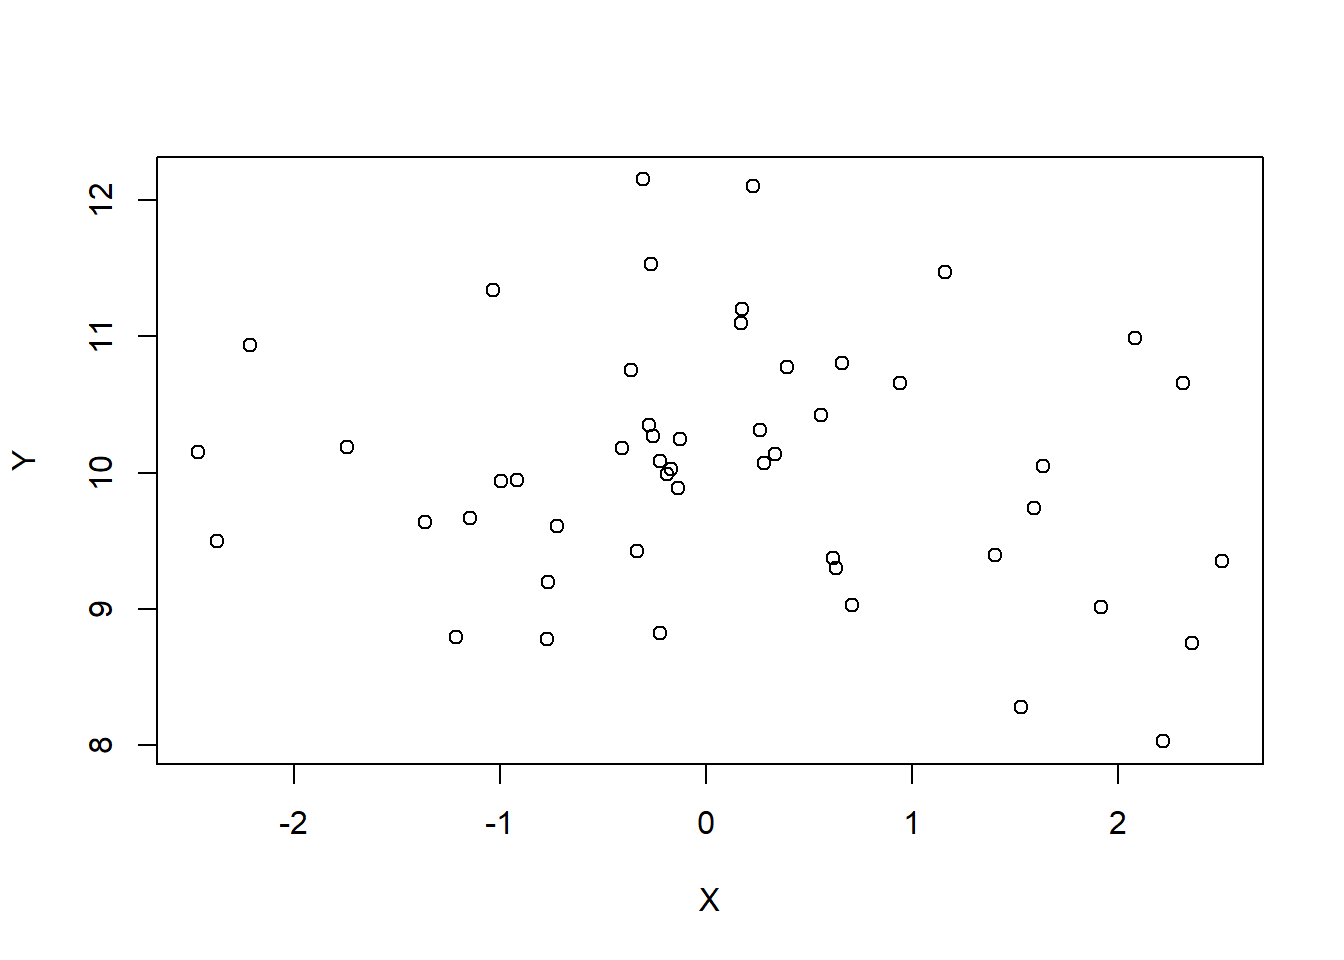
\includegraphics{myRBook_SP_files/figure-latex/unnamed-chunk-220-1.pdf}

Al igual que con todos los tipos de gráficos, podemos agregar una
leyenda en los ejes x e y.

\begin{Shaded}
\begin{Highlighting}[]
\KeywordTok{plot}\NormalTok{(}\DataTypeTok{x =}\NormalTok{ myX, }\DataTypeTok{y =}\NormalTok{ myY, }
  \DataTypeTok{xlab =} \StringTok{"X"}\NormalTok{, }\DataTypeTok{ylab =} \StringTok{"Y"}\NormalTok{)}
\end{Highlighting}
\end{Shaded}

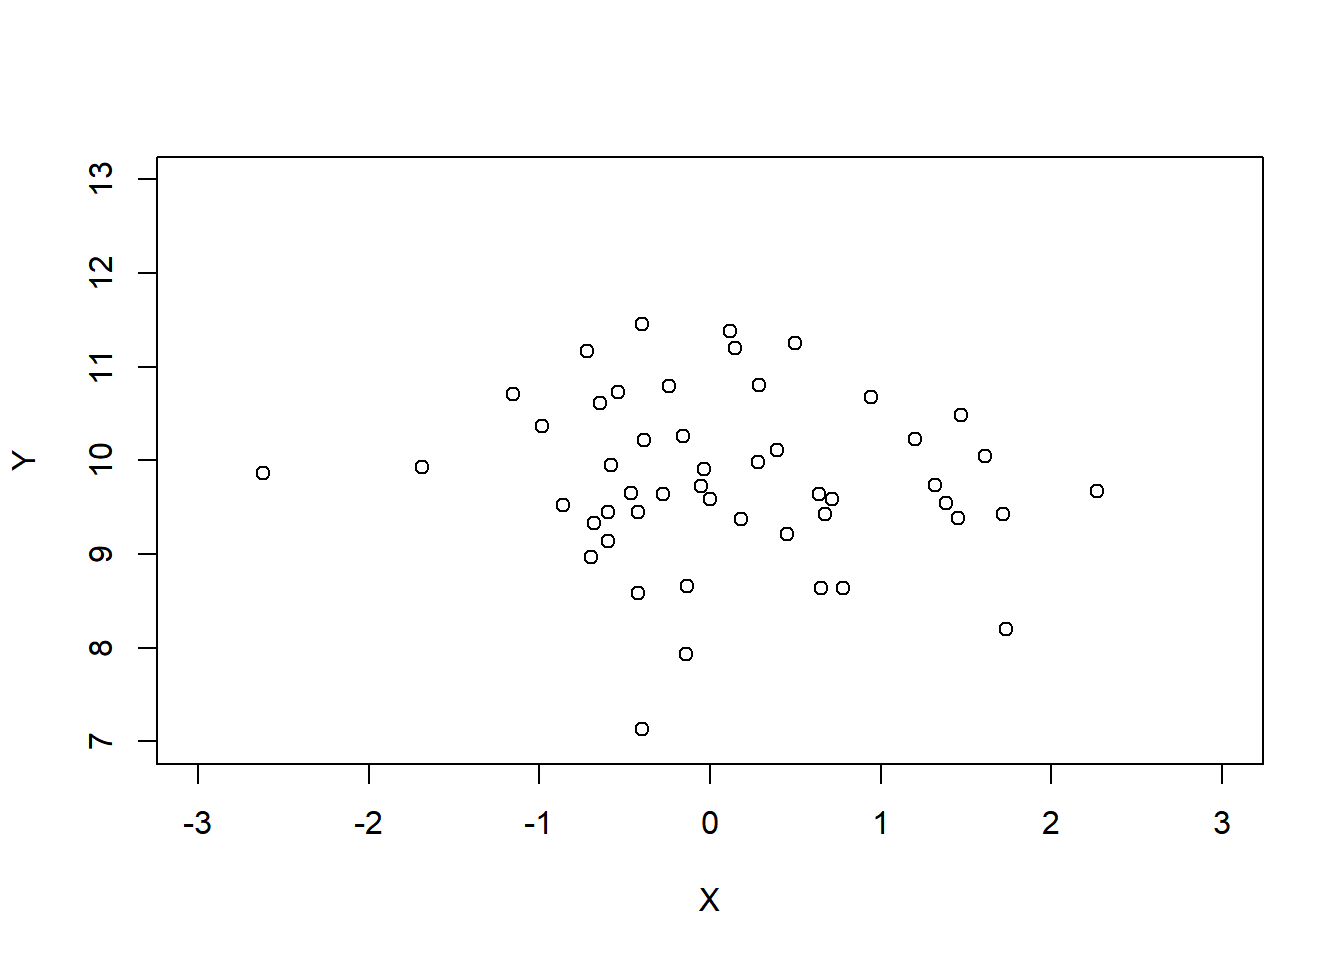
\includegraphics{myRBook_SP_files/figure-latex/unnamed-chunk-221-1.pdf}

También podemos definir los límites de los ejes X e Y.

\begin{Shaded}
\begin{Highlighting}[]
\KeywordTok{plot}\NormalTok{(}\DataTypeTok{x =}\NormalTok{ myX, }\DataTypeTok{y =}\NormalTok{ myY, }
  \DataTypeTok{xlab =} \StringTok{"X"}\NormalTok{, }\DataTypeTok{ylab =} \StringTok{"Y"}\NormalTok{, }
  \DataTypeTok{xlim =} \KeywordTok{c}\NormalTok{(}\OperatorTok{-}\DecValTok{3}\NormalTok{, }\DecValTok{3}\NormalTok{), }\DataTypeTok{ylim =} \KeywordTok{c}\NormalTok{(}\DecValTok{7}\NormalTok{, }\DecValTok{13}\NormalTok{))}
\end{Highlighting}
\end{Shaded}

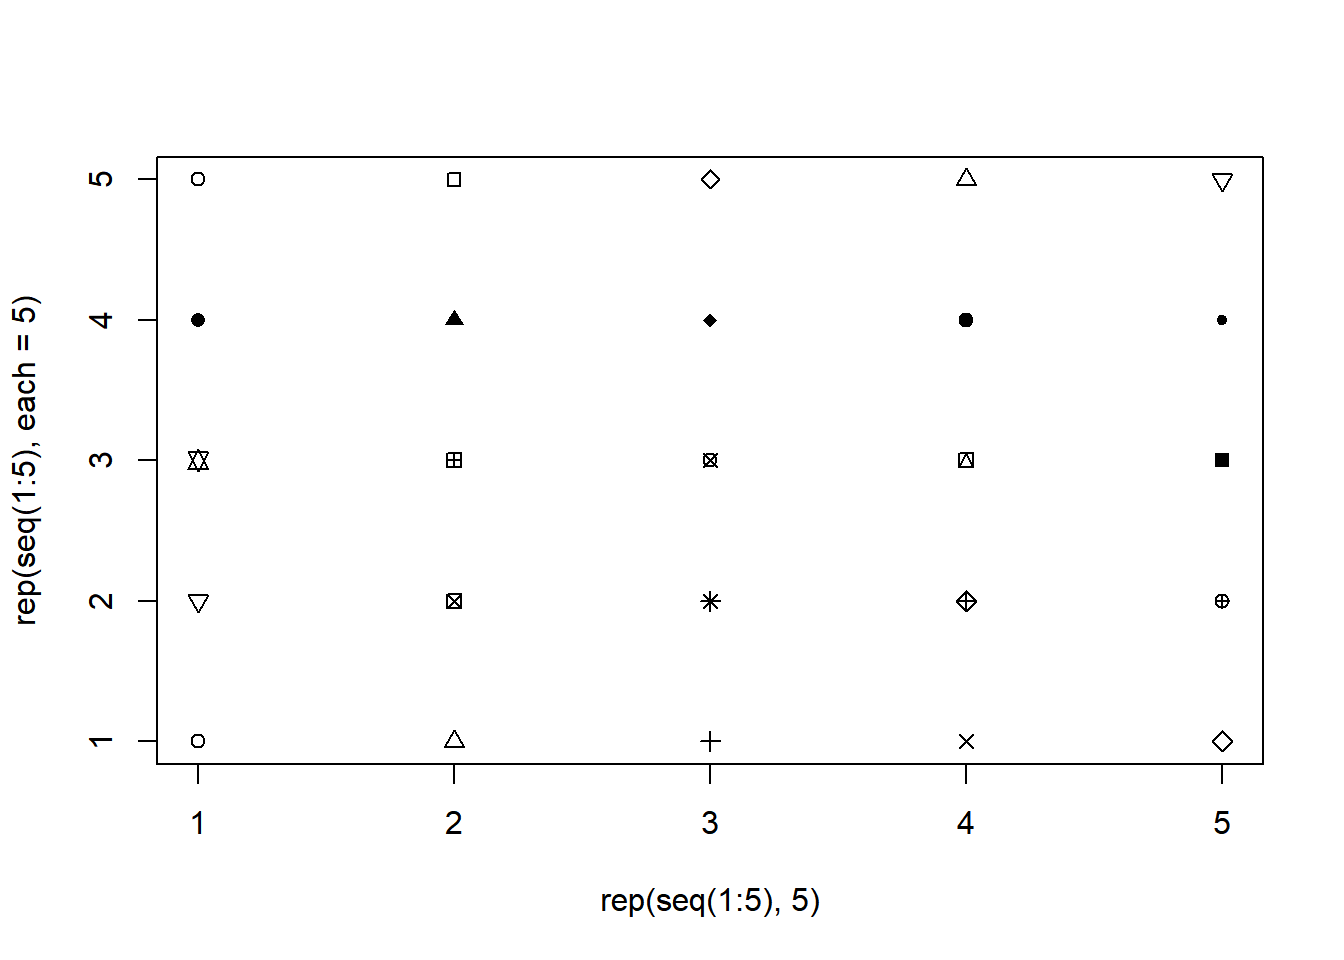
\includegraphics{myRBook_SP_files/figure-latex/unnamed-chunk-222-1.pdf}

El tipo de punto se puede establecer con el argumento \texttt{pch} que
puede tomar un carácter o un número del 1 al 25.

\begin{Shaded}
\begin{Highlighting}[]
\KeywordTok{plot}\NormalTok{(}\DataTypeTok{x =} \KeywordTok{rep}\NormalTok{(}\KeywordTok{seq}\NormalTok{(}\DecValTok{1}\OperatorTok{:}\DecValTok{5}\NormalTok{), }\DecValTok{5}\NormalTok{), }\DataTypeTok{y =} \KeywordTok{rep}\NormalTok{(}\KeywordTok{seq}\NormalTok{(}\DecValTok{1}\OperatorTok{:}\DecValTok{5}\NormalTok{), }\DataTypeTok{each =} \DecValTok{5}\NormalTok{),}
  \DataTypeTok{pch =} \DecValTok{1}\OperatorTok{:}\DecValTok{25}\NormalTok{)}
\end{Highlighting}
\end{Shaded}

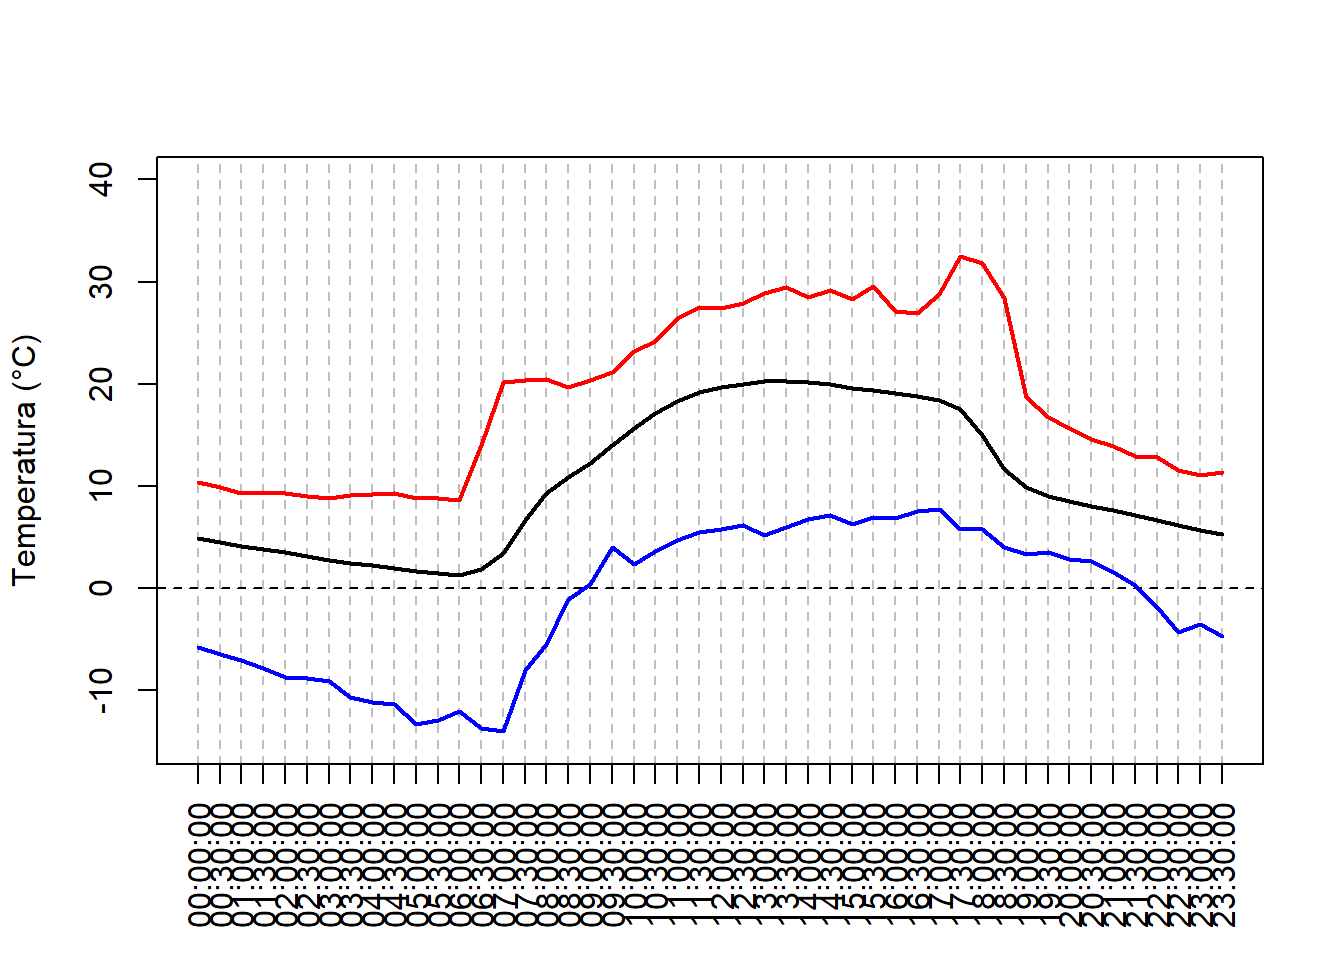
\includegraphics{myRBook_SP_files/figure-latex/unnamed-chunk-223-1.pdf}

\begin{Shaded}
\begin{Highlighting}[]
\KeywordTok{plot}\NormalTok{(}\DataTypeTok{x =}\NormalTok{ myX, }\DataTypeTok{y =}\NormalTok{ myY, }
  \DataTypeTok{pch =} \KeywordTok{c}\NormalTok{(}\StringTok{"a"}\NormalTok{, }\StringTok{"@"}\NormalTok{, }\StringTok{"#"}\NormalTok{, }\StringTok{"1"}\NormalTok{, }\StringTok{"="}\NormalTok{, }\StringTok{"-"}\NormalTok{, }\StringTok{"_"}\NormalTok{, }\StringTok{"o"}\NormalTok{, }\StringTok{"O"}\NormalTok{, }\StringTok{"0"}\NormalTok{, letters[}\DecValTok{1}\OperatorTok{:}\DecValTok{15}\NormalTok{]))}
\end{Highlighting}
\end{Shaded}

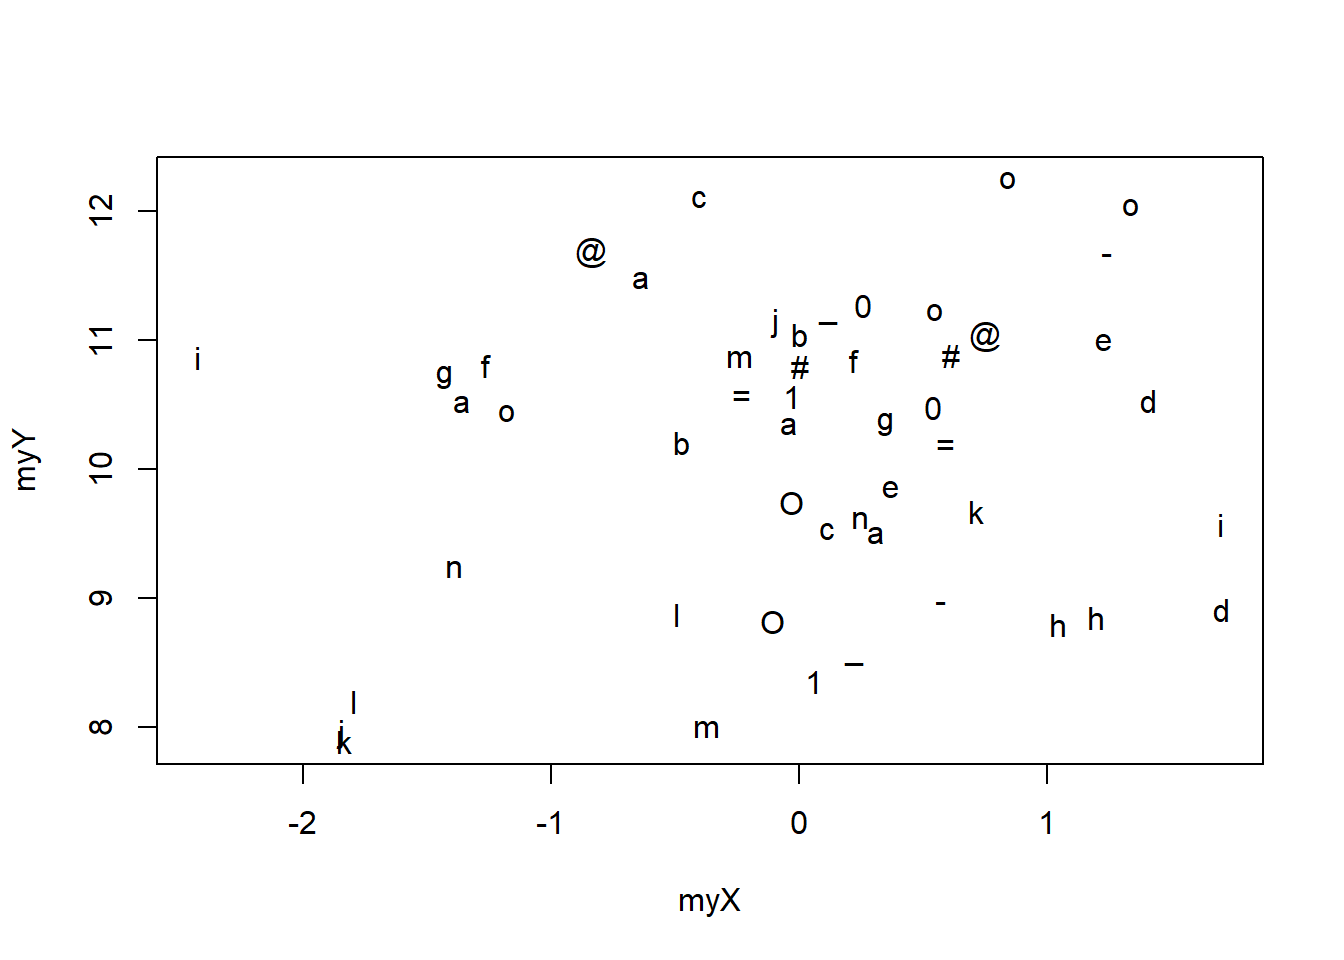
\includegraphics{myRBook_SP_files/figure-latex/unnamed-chunk-223-2.pdf}

El tamaño de los puntos se puede definir con el argumento \texttt{cex}.

\begin{Shaded}
\begin{Highlighting}[]
\KeywordTok{plot}\NormalTok{(}\DataTypeTok{x =}\NormalTok{ myX, }\DataTypeTok{y =}\NormalTok{ myY, }
  \DataTypeTok{cex =} \KeywordTok{seq}\NormalTok{(}\DataTypeTok{from =} \FloatTok{0.5}\NormalTok{, }\DataTypeTok{to =} \DecValTok{3}\NormalTok{, }\DataTypeTok{length.out =} \DecValTok{50}\NormalTok{))}
\end{Highlighting}
\end{Shaded}

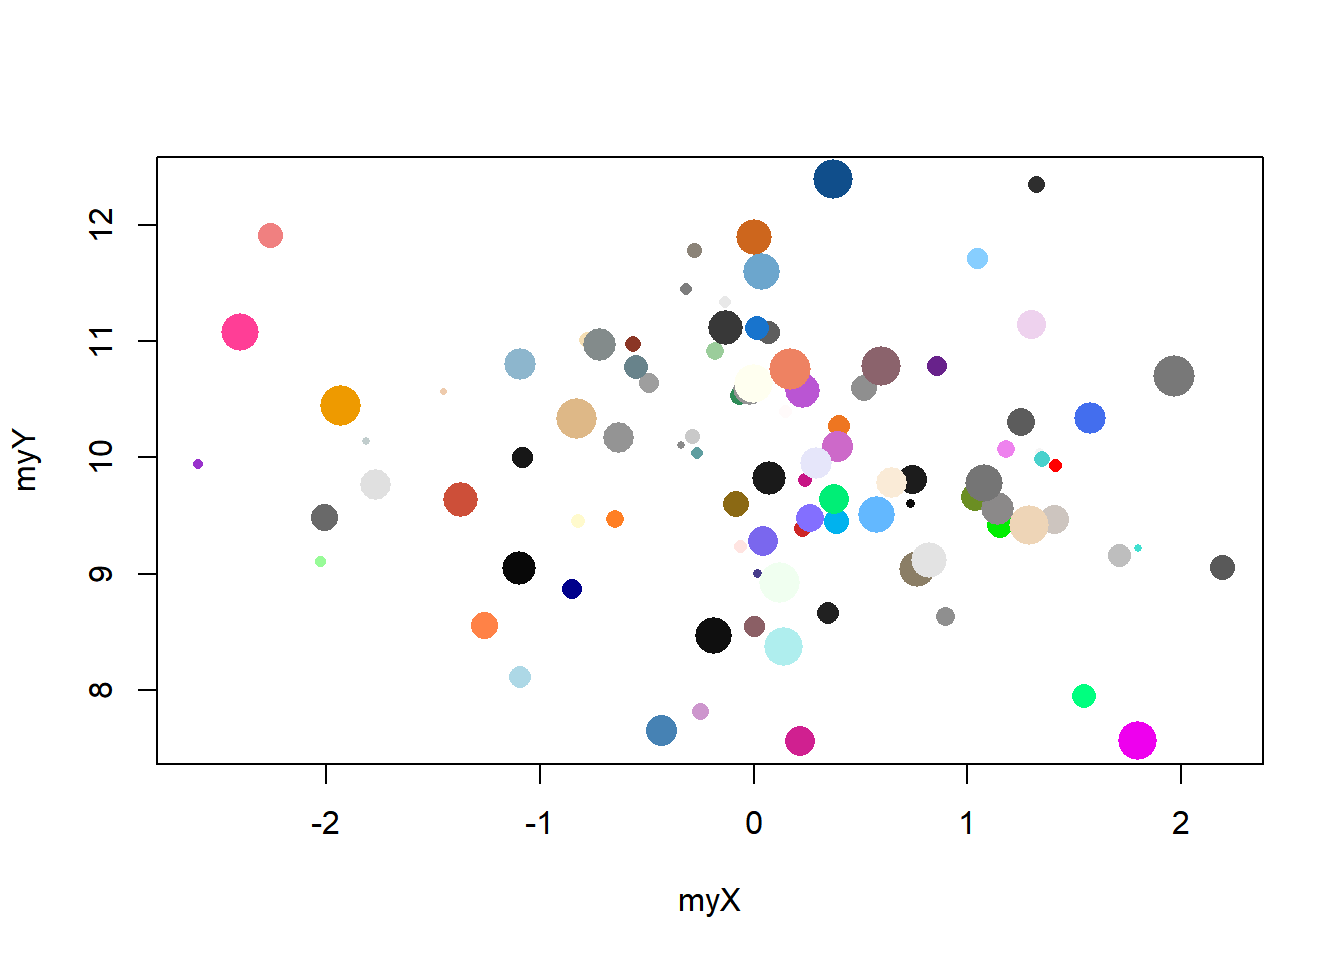
\includegraphics{myRBook_SP_files/figure-latex/unnamed-chunk-224-1.pdf}

El color de los puntos se puede definir con el argumento \texttt{col}.
Volveremos a los colores en un próximo capítulo.

\begin{Shaded}
\begin{Highlighting}[]
\NormalTok{myX <-}\StringTok{ }\KeywordTok{rnorm}\NormalTok{(}\DecValTok{100}\NormalTok{, }\DataTypeTok{mean =} \DecValTok{0}\NormalTok{, }\DataTypeTok{sd =} \DecValTok{1}\NormalTok{)}
\NormalTok{myY <-}\StringTok{ }\KeywordTok{rnorm}\NormalTok{(}\DecValTok{100}\NormalTok{, }\DataTypeTok{mean =} \DecValTok{10}\NormalTok{, }\DataTypeTok{sd =} \DecValTok{1}\NormalTok{)}
\KeywordTok{plot}\NormalTok{(}\DataTypeTok{x =}\NormalTok{ myX, }\DataTypeTok{y =}\NormalTok{ myY, }
  \DataTypeTok{cex =} \KeywordTok{seq}\NormalTok{(}\DataTypeTok{from =} \FloatTok{0.5}\NormalTok{, }\DataTypeTok{to =} \DecValTok{3}\NormalTok{, }\DataTypeTok{length.out =} \DecValTok{100}\NormalTok{),}
  \DataTypeTok{pch =} \DecValTok{16}\NormalTok{,}
  \DataTypeTok{col =} \KeywordTok{sample}\NormalTok{(}\KeywordTok{colors}\NormalTok{(), }\DecValTok{100}\NormalTok{))}
\end{Highlighting}
\end{Shaded}

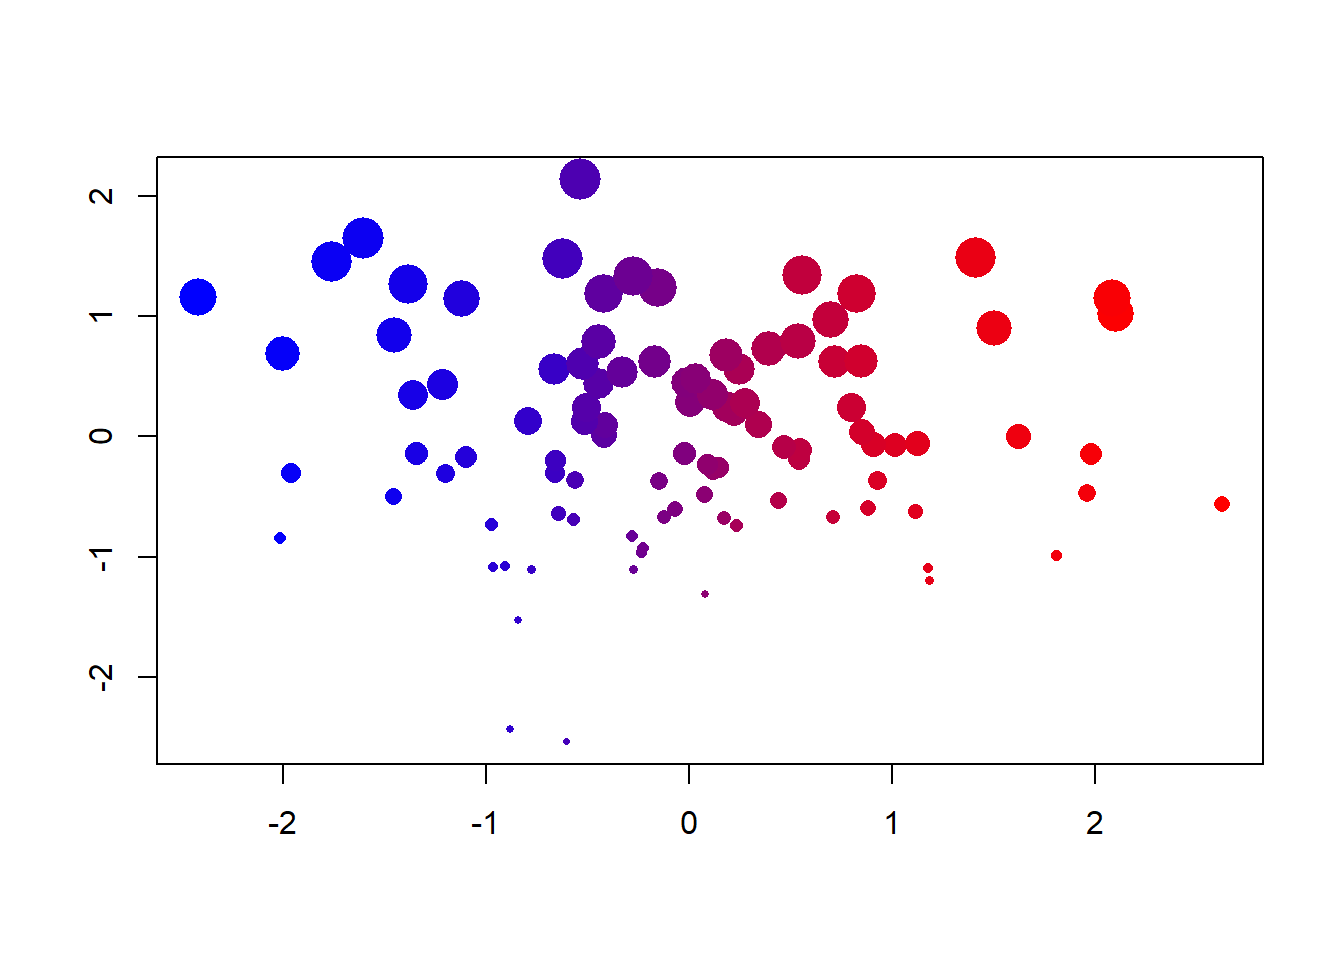
\includegraphics{myRBook_SP_files/figure-latex/unnamed-chunk-225-1.pdf}

Para representar nuestros puntos, el color y el tamaño de los puntos
pueden representar información adicional. Aquí representaremos por un
gradiente de tamaño la variable \texttt{myY} y por un gradiente de color
la variable\texttt{myX}.

\begin{Shaded}
\begin{Highlighting}[]
\NormalTok{myX <-}\StringTok{ }\KeywordTok{rnorm}\NormalTok{(}\DecValTok{100}\NormalTok{)}
\NormalTok{myY <-}\StringTok{ }\KeywordTok{rnorm}\NormalTok{(}\DecValTok{100}\NormalTok{)}
\NormalTok{dfGraph <-}\StringTok{ }\KeywordTok{data.frame}\NormalTok{(myX, myY)}
\NormalTok{dfGraph <-}\StringTok{ }\NormalTok{dfGraph[}\KeywordTok{order}\NormalTok{(dfGraph}\OperatorTok{$}\NormalTok{myX),]}
\NormalTok{dfGraph}\OperatorTok{$}\NormalTok{myCol <-}\StringTok{ }\KeywordTok{colorRampPalette}\NormalTok{(}\KeywordTok{c}\NormalTok{(}\StringTok{"blue"}\NormalTok{, }\StringTok{"red"}\NormalTok{))(}\DecValTok{100}\NormalTok{)}
\NormalTok{dfGraph <-}\StringTok{ }\NormalTok{dfGraph[}\KeywordTok{order}\NormalTok{(dfGraph}\OperatorTok{$}\NormalTok{myY),]}
\NormalTok{dfGraph}\OperatorTok{$}\NormalTok{myCex <-}\StringTok{ }\KeywordTok{seq}\NormalTok{(}\DataTypeTok{from =} \FloatTok{0.5}\NormalTok{, }\DataTypeTok{to =} \DecValTok{3}\NormalTok{, }\DataTypeTok{length.out =} \DecValTok{100}\NormalTok{)}
\KeywordTok{plot}\NormalTok{(}\DataTypeTok{x =}\NormalTok{ dfGraph}\OperatorTok{$}\NormalTok{myX, }\DataTypeTok{y =}\NormalTok{ dfGraph}\OperatorTok{$}\NormalTok{myY, }
  \DataTypeTok{cex =}\NormalTok{ dfGraph}\OperatorTok{$}\NormalTok{myCex, }\DataTypeTok{pch =} \DecValTok{16}\NormalTok{, }\DataTypeTok{col =}\NormalTok{ dfGraph}\OperatorTok{$}\NormalTok{myCol, }
  \DataTypeTok{xlab =} \StringTok{""}\NormalTok{, }\DataTypeTok{ylab =} \StringTok{""}\NormalTok{)}
\end{Highlighting}
\end{Shaded}

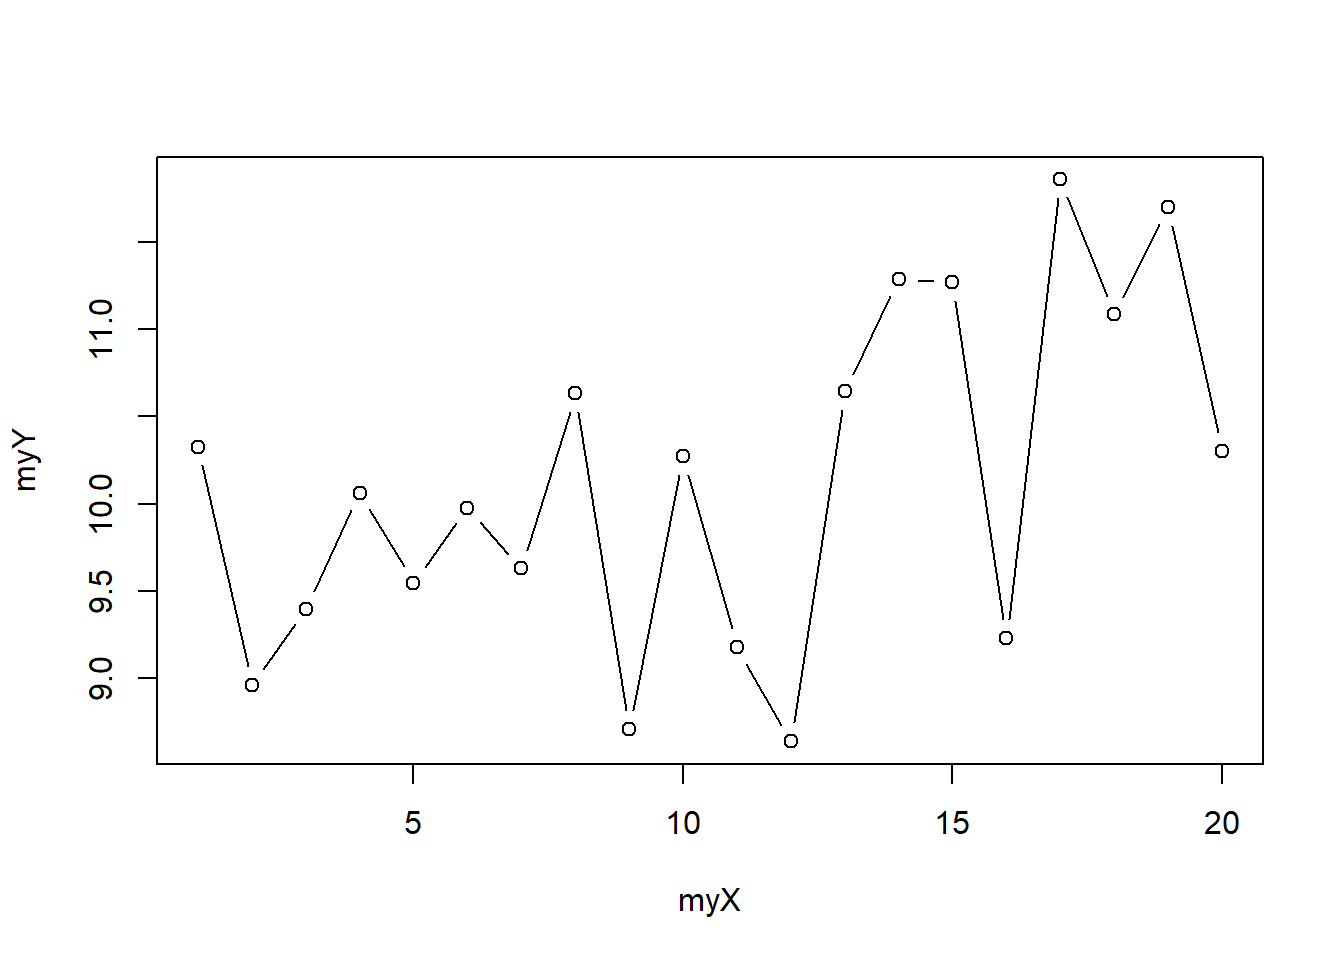
\includegraphics{myRBook_SP_files/figure-latex/unnamed-chunk-226-1.pdf}

R ofrece la posibilidad de conectar puntos de nube de puntos de
diferentes maneras. Las diferentes opciones están disponibles en la
ayuda de las funciones \texttt{plot()} y \texttt{plot.default()}.

\begin{Shaded}
\begin{Highlighting}[]
\NormalTok{myX <-}\StringTok{ }\DecValTok{1}\OperatorTok{:}\DecValTok{20}
\NormalTok{myY <-}\StringTok{ }\KeywordTok{rnorm}\NormalTok{(}\DecValTok{20}\NormalTok{, }\DataTypeTok{mean =} \DecValTok{10}\NormalTok{, }\DataTypeTok{sd =} \DecValTok{1}\NormalTok{)}
\KeywordTok{plot}\NormalTok{(}\DataTypeTok{x =}\NormalTok{ myX, }\DataTypeTok{y =}\NormalTok{ myY, }
  \DataTypeTok{type =} \StringTok{'b'}\NormalTok{) }\CommentTok{# 'p', 'l', 'b', 'c', 'o', 'h', 's', 'S', 'n'}
\end{Highlighting}
\end{Shaded}

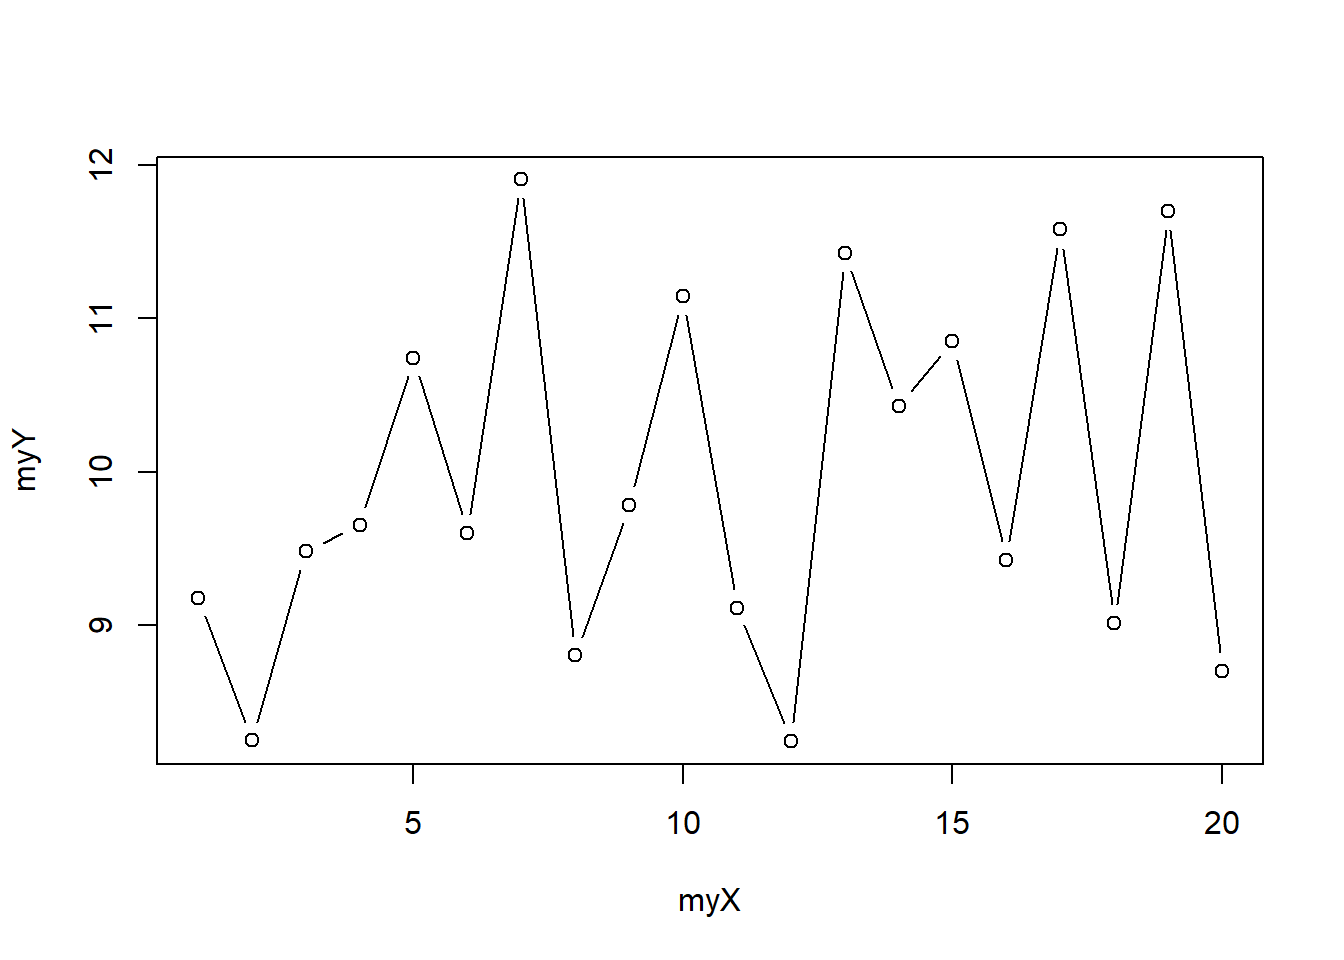
\includegraphics{myRBook_SP_files/figure-latex/unnamed-chunk-227-1.pdf}

Una última opción muy útil es el argumento \texttt{panel.first} que
permite realizar una operación gráfica en una capa debajo de nuestro
gráfico. Aquí hay un ejemplo ilustrativo con una cuadrícula hecha con y
sin \texttt{panel.first}. La cuadrícula se realiza gracias a la función
\texttt{grid()}. Para poner los gráficos lado a lado usaremos
\texttt{mfrow}.

\begin{Shaded}
\begin{Highlighting}[]
\KeywordTok{par}\NormalTok{(}\DataTypeTok{mfrow =} \KeywordTok{c}\NormalTok{(}\DecValTok{1}\NormalTok{, }\DecValTok{2}\NormalTok{))}
\KeywordTok{plot}\NormalTok{(}\DataTypeTok{x =}\NormalTok{ myX, }\DataTypeTok{y =}\NormalTok{ myY, }
  \DataTypeTok{type =} \StringTok{'b'}\NormalTok{, }\DataTypeTok{pch =} \DecValTok{16}\NormalTok{, }\DataTypeTok{cex =} \DecValTok{3}\NormalTok{) }
\KeywordTok{grid}\NormalTok{(}\DataTypeTok{lwd =} \DecValTok{3}\NormalTok{, }\DataTypeTok{lty =} \DecValTok{1}\NormalTok{)}
\KeywordTok{plot}\NormalTok{(}\DataTypeTok{x =}\NormalTok{ myX, }\DataTypeTok{y =}\NormalTok{ myY, }
  \DataTypeTok{type =} \StringTok{'b'}\NormalTok{, }\DataTypeTok{pch =} \DecValTok{16}\NormalTok{, }\DataTypeTok{cex =} \DecValTok{3}\NormalTok{, }
  \DataTypeTok{panel.first =} \KeywordTok{grid}\NormalTok{(}\DataTypeTok{lwd =} \DecValTok{3}\NormalTok{, }\DataTypeTok{lty =} \DecValTok{1}\NormalTok{)) }
\end{Highlighting}
\end{Shaded}

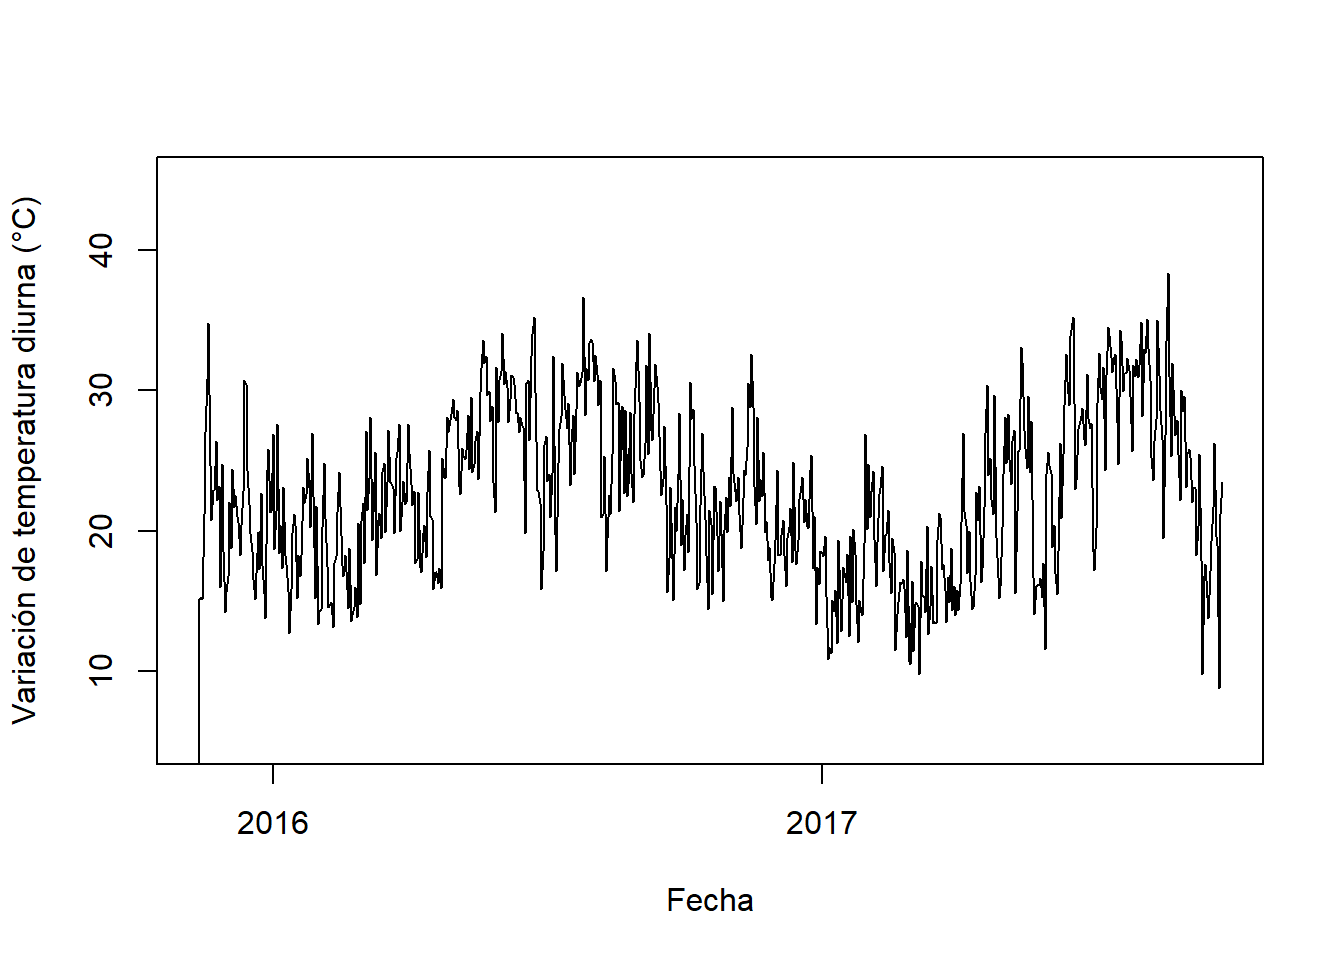
\includegraphics{myRBook_SP_files/figure-latex/unnamed-chunk-228-1.pdf}

\begin{Shaded}
\begin{Highlighting}[]
\KeywordTok{par}\NormalTok{(}\DataTypeTok{mfrow =} \KeywordTok{c}\NormalTok{(}\DecValTok{1}\NormalTok{, }\DecValTok{1}\NormalTok{))}
\end{Highlighting}
\end{Shaded}

La función \texttt{par()} proporciona acceso a parámetros gráficos.
Entre estos parámetros hay \texttt{mfrow} que permite dividir el espacio
gráfico como una matriz. \texttt{mfrow} toma como argumentos un vector
numérico de tamaño 2: el primer elemento corresponde al número de líneas
y el segundo elemento al número de columnas. El parámetro \texttt{mar}
controla los márgenes en la parte inferior, izquierda, superior y
derecha, respectivamente, utilizando un vector digital de tamaño 4.
Después de cambiar la configuración de gráficos predeterminada, se
recomienda restablecerlos para que no afecte a los futuros gráficos. Los
valores predeterminados para \texttt{mfrow} son \texttt{c(1,\ 1)} y
\texttt{mar\ =\ c\ (4,\ 4,\ 4,\ 4)}. Podemos restablecer estos valores
predeterminados como antes, redefiniendo cada parámetro. También podemos
guardar los valores actuales (en un objeto \texttt{op}) de antemano,
modificarlos para los propósitos de nuestros gráficos y luego recuperar
los valores contenidos en el objeto \texttt{op}. Aquí usamos
\texttt{lapply} para hacer rápidamente cuatro gráficos.

\begin{Shaded}
\begin{Highlighting}[]
\NormalTok{op <-}\StringTok{ }\KeywordTok{par}\NormalTok{(}\DataTypeTok{no.readonly =} \OtherTok{TRUE}\NormalTok{)}
\KeywordTok{par}\NormalTok{(}\DataTypeTok{mfrow =} \KeywordTok{c}\NormalTok{(}\DecValTok{2}\NormalTok{, }\DecValTok{2}\NormalTok{), }\DataTypeTok{mar =} \KeywordTok{c}\NormalTok{(}\DecValTok{2}\NormalTok{, }\DecValTok{2}\NormalTok{, }\DecValTok{1}\NormalTok{, }\DecValTok{1}\NormalTok{))}
\NormalTok{graph4 <-}\StringTok{ }\KeywordTok{lapply}\NormalTok{(}\DecValTok{1}\OperatorTok{:}\DecValTok{4}\NormalTok{, }\ControlFlowTok{function}\NormalTok{(i)\{}
  \KeywordTok{plot}\NormalTok{(}\DataTypeTok{x =} \KeywordTok{rnorm}\NormalTok{(}\DecValTok{100}\NormalTok{), }
    \DataTypeTok{y =} \KeywordTok{rnorm}\NormalTok{(}\DecValTok{100}\NormalTok{), }
    \DataTypeTok{col =}\NormalTok{ i, }\DataTypeTok{pch =} \DecValTok{16}\NormalTok{)}
\NormalTok{\})}
\end{Highlighting}
\end{Shaded}

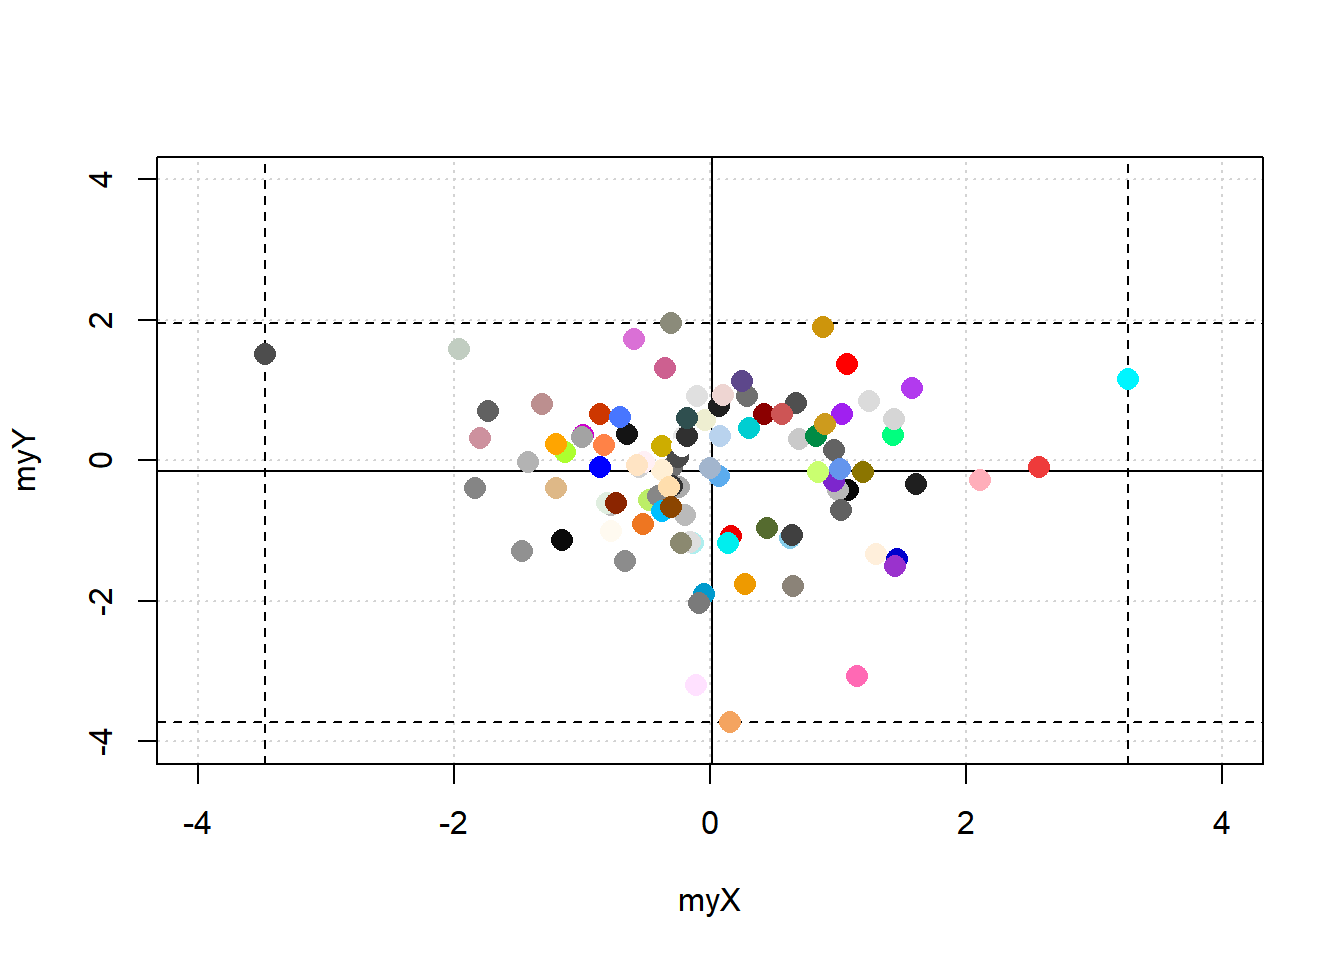
\includegraphics{myRBook_SP_files/figure-latex/unnamed-chunk-229-1.pdf}

\begin{Shaded}
\begin{Highlighting}[]
\KeywordTok{par}\NormalTok{(op)}
\end{Highlighting}
\end{Shaded}

Es útil incluir líneas verticales u horizontales para representar
valores particulares. Estas líneas se pueden agregar con la función
\texttt{abline()}.

\begin{Shaded}
\begin{Highlighting}[]
\NormalTok{myX <-}\StringTok{ }\KeywordTok{rnorm}\NormalTok{(}\DecValTok{100}\NormalTok{)}
\NormalTok{myY <-}\StringTok{ }\KeywordTok{rnorm}\NormalTok{(}\DecValTok{100}\NormalTok{)}
\KeywordTok{plot}\NormalTok{(}\DataTypeTok{x =}\NormalTok{ myX, }\DataTypeTok{y =}\NormalTok{ myY, }
  \DataTypeTok{xlim =} \KeywordTok{c}\NormalTok{(}\OperatorTok{-}\DecValTok{4}\NormalTok{, }\DecValTok{4}\NormalTok{), }\DataTypeTok{ylim =} \KeywordTok{c}\NormalTok{(}\OperatorTok{-}\DecValTok{4}\NormalTok{, }\DecValTok{4}\NormalTok{),   }
  \DataTypeTok{pch =} \DecValTok{16}\NormalTok{, }\DataTypeTok{cex =} \FloatTok{1.5}\NormalTok{, }
  \DataTypeTok{col =} \KeywordTok{sample}\NormalTok{(}\KeywordTok{colors}\NormalTok{(), }\DataTypeTok{size =} \DecValTok{100}\NormalTok{),}
  \DataTypeTok{panel.first =}\NormalTok{ \{}
    \KeywordTok{grid}\NormalTok{()}
    \KeywordTok{abline}\NormalTok{(}\DataTypeTok{v =} \KeywordTok{c}\NormalTok{(}\KeywordTok{min}\NormalTok{(myX), }\KeywordTok{max}\NormalTok{(myX)), }\DataTypeTok{lty =} \DecValTok{2}\NormalTok{)}
    \KeywordTok{abline}\NormalTok{(}\DataTypeTok{h =} \KeywordTok{c}\NormalTok{(}\KeywordTok{min}\NormalTok{(myY), }\KeywordTok{max}\NormalTok{(myY)), }\DataTypeTok{lty =} \DecValTok{2}\NormalTok{)}
    \KeywordTok{abline}\NormalTok{(}\DataTypeTok{v =} \KeywordTok{mean}\NormalTok{(myX), }\DataTypeTok{lty =} \DecValTok{1}\NormalTok{)}
    \KeywordTok{abline}\NormalTok{(}\DataTypeTok{h =} \KeywordTok{mean}\NormalTok{(myY), }\DataTypeTok{lty =} \DecValTok{1}\NormalTok{)}
\NormalTok{\})}
\end{Highlighting}
\end{Shaded}

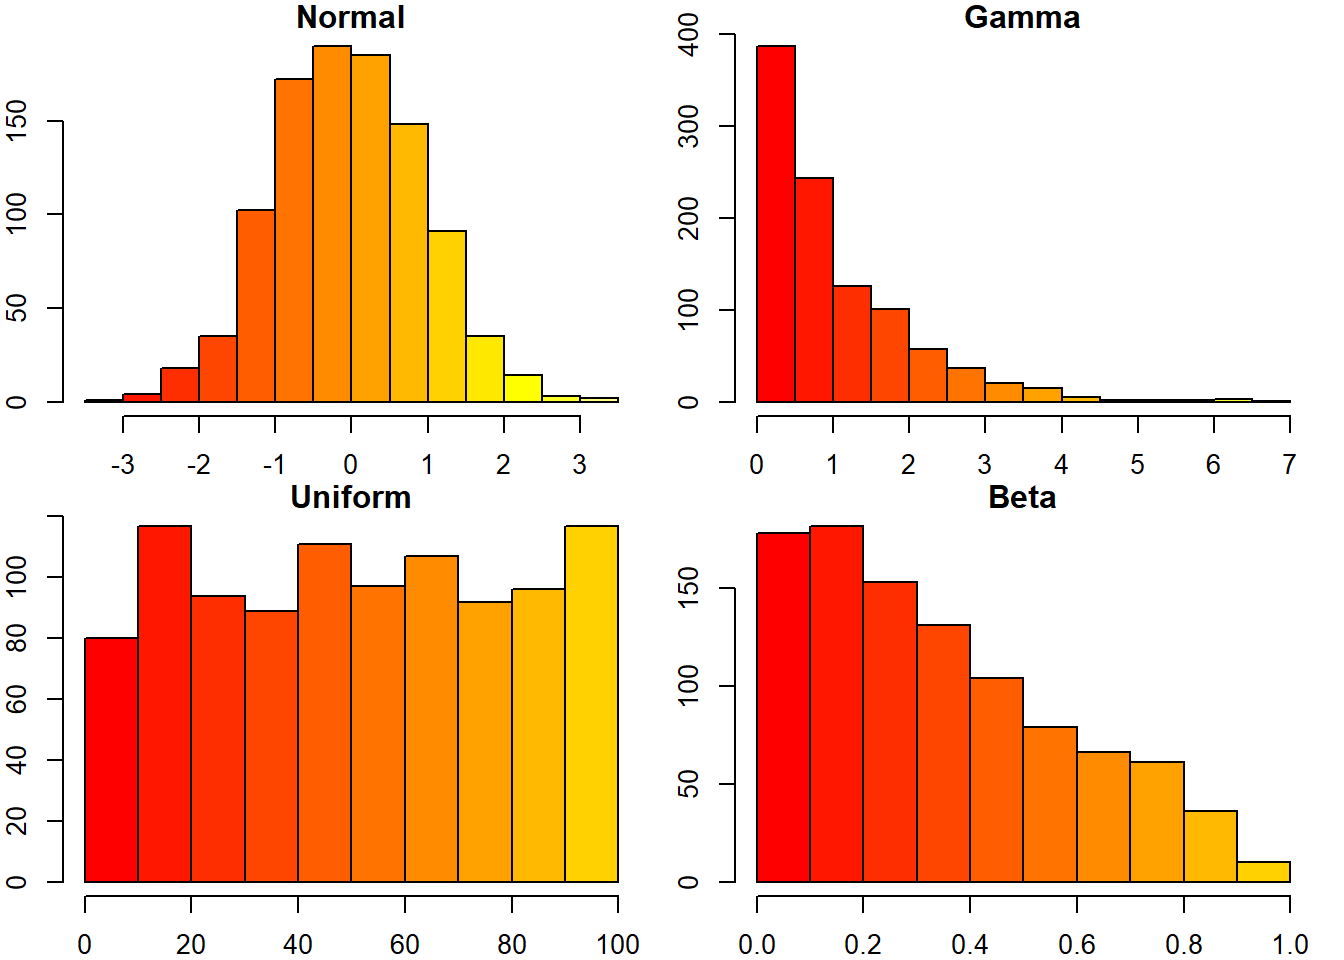
\includegraphics{myRBook_SP_files/figure-latex/unnamed-chunk-230-1.pdf}

\section{\texorpdfstring{\texttt{hist}}{hist}}\label{graph1hist}

Para hacer un histograma usamos la función \texttt{hist()}. Esta es una
función gráfica útil para visualizar rápidamente la distribución de un
conjunto de datos.

\begin{Shaded}
\begin{Highlighting}[]
\NormalTok{op <-}\StringTok{ }\KeywordTok{par}\NormalTok{(}\DataTypeTok{no.readonly =} \OtherTok{TRUE}\NormalTok{)}
\KeywordTok{par}\NormalTok{(}\DataTypeTok{mfrow =} \KeywordTok{c}\NormalTok{(}\DecValTok{2}\NormalTok{, }\DecValTok{2}\NormalTok{), }\DataTypeTok{mar =} \KeywordTok{c}\NormalTok{(}\DecValTok{2}\NormalTok{, }\DecValTok{2}\NormalTok{, }\DecValTok{1}\NormalTok{, }\DecValTok{1}\NormalTok{))}
\NormalTok{myX <-}\StringTok{ }\KeywordTok{list}\NormalTok{(}
  \KeywordTok{rnorm}\NormalTok{(}\DecValTok{1000}\NormalTok{),}
  \KeywordTok{rgamma}\NormalTok{(}\DecValTok{1000}\NormalTok{, }\DataTypeTok{shape =} \DecValTok{1}\NormalTok{),}
  \KeywordTok{sample}\NormalTok{(}\DecValTok{1}\OperatorTok{:}\DecValTok{100}\NormalTok{, }\DataTypeTok{size =} \DecValTok{1000}\NormalTok{, }\DataTypeTok{replace =} \OtherTok{TRUE}\NormalTok{),}
  \KeywordTok{rbeta}\NormalTok{(}\DecValTok{1000}\NormalTok{, }\DataTypeTok{shape1 =} \DecValTok{1}\NormalTok{, }\DataTypeTok{shape2 =} \DecValTok{2}\NormalTok{)}
\NormalTok{)}
\NormalTok{myTitle <-}\StringTok{ }\KeywordTok{c}\NormalTok{(}\StringTok{"Normal"}\NormalTok{, }\StringTok{"Gamma"}\NormalTok{, }\StringTok{"Uniform"}\NormalTok{, }\StringTok{"Beta"}\NormalTok{)}
\NormalTok{tr <-}\StringTok{ }\KeywordTok{lapply}\NormalTok{(}\DecValTok{1}\OperatorTok{:}\DecValTok{4}\NormalTok{, }\ControlFlowTok{function}\NormalTok{(i)\{}
  \KeywordTok{hist}\NormalTok{(myX[[i]], }
    \DataTypeTok{col =} \KeywordTok{heat.colors}\NormalTok{(}\DecValTok{15}\NormalTok{), }
    \DataTypeTok{main =}\NormalTok{ myTitle[i]}
\NormalTok{  )}
\NormalTok{\})}
\end{Highlighting}
\end{Shaded}

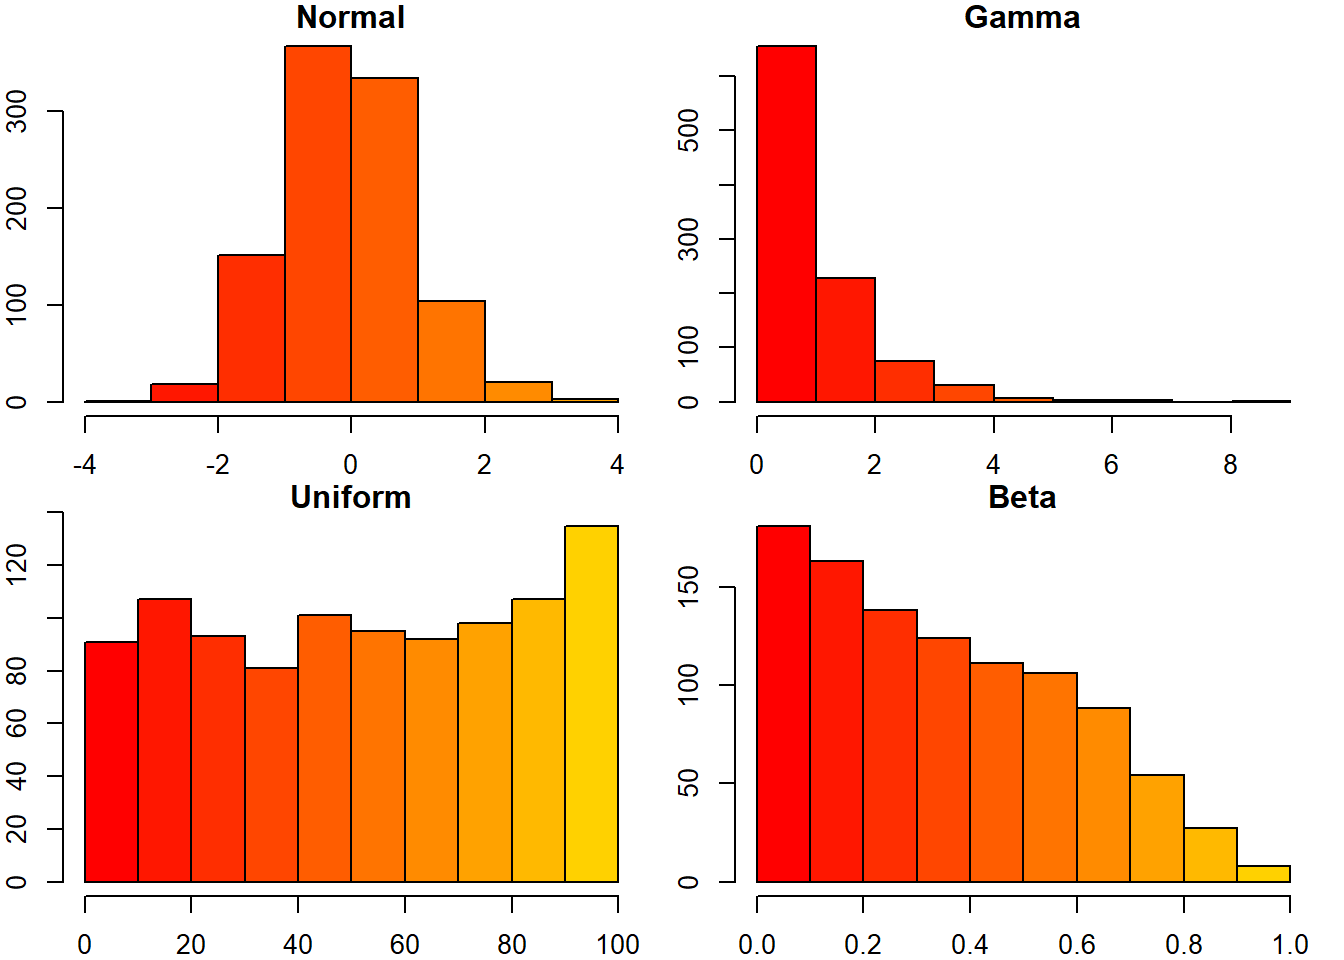
\includegraphics{myRBook_SP_files/figure-latex/unnamed-chunk-231-1.pdf}

\begin{Shaded}
\begin{Highlighting}[]
\KeywordTok{par}\NormalTok{(op)}
\end{Highlighting}
\end{Shaded}

\section{\texorpdfstring{\texttt{barplot}}{barplot}}\label{graph1barplot}

El gráfico de barras se realiza utilizando la función
\texttt{barplot()}.

\begin{Shaded}
\begin{Highlighting}[]
\NormalTok{myX <-}\StringTok{ }\KeywordTok{c}\NormalTok{(}\DecValTok{4}\NormalTok{, }\DecValTok{5}\NormalTok{, }\DecValTok{8}\NormalTok{)}
\KeywordTok{barplot}\NormalTok{(myX, }\DataTypeTok{names.arg =} \KeywordTok{c}\NormalTok{(}\StringTok{"A"}\NormalTok{, }\StringTok{"B"}\NormalTok{, }\StringTok{"C"}\NormalTok{))}
\end{Highlighting}
\end{Shaded}

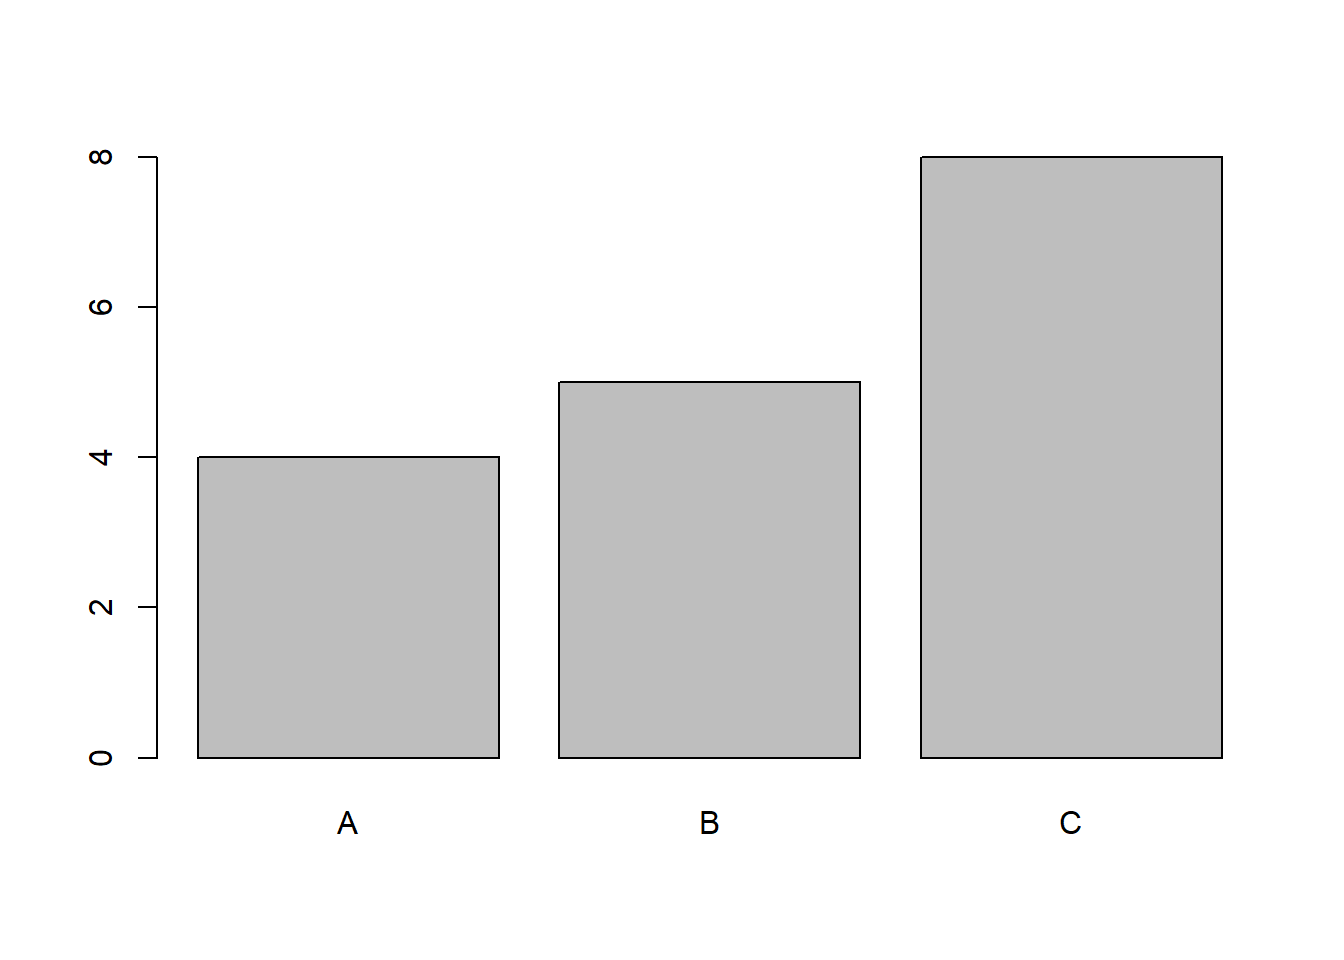
\includegraphics{myRBook_SP_files/figure-latex/unnamed-chunk-232-1.pdf}

Cuando el objeto enviado a esta función es un \texttt{vector}, entonces
la función \texttt{barplot()} devuelve un gráfico de barras simple.
Cuando es un \texttt{matrix} entonces las barras son múltiples.

\begin{Shaded}
\begin{Highlighting}[]
\NormalTok{op <-}\StringTok{ }\KeywordTok{par}\NormalTok{(}\DataTypeTok{no.readonly =} \OtherTok{TRUE}\NormalTok{)}
\KeywordTok{par}\NormalTok{(}\DataTypeTok{mfrow =} \KeywordTok{c}\NormalTok{(}\DecValTok{1}\NormalTok{, }\DecValTok{2}\NormalTok{), }\DataTypeTok{mar =} \KeywordTok{c}\NormalTok{(}\DecValTok{2}\NormalTok{, }\DecValTok{2}\NormalTok{, }\DecValTok{1}\NormalTok{, }\DecValTok{1}\NormalTok{))}
\NormalTok{myX <-}\StringTok{ }\KeywordTok{matrix}\NormalTok{(}\KeywordTok{c}\NormalTok{(}\DecValTok{4}\NormalTok{, }\DecValTok{5}\NormalTok{, }\DecValTok{8}\NormalTok{, }\DecValTok{4}\NormalTok{, }\DecValTok{6}\NormalTok{, }\DecValTok{2}\NormalTok{), }\DataTypeTok{nrow =} \DecValTok{2}\NormalTok{)}
\KeywordTok{barplot}\NormalTok{(myX, }\DataTypeTok{names.arg =} \KeywordTok{c}\NormalTok{(}\StringTok{"A"}\NormalTok{, }\StringTok{"B"}\NormalTok{, }\StringTok{"C"}\NormalTok{))}
\NormalTok{myX <-}\StringTok{ }\KeywordTok{matrix}\NormalTok{(}\KeywordTok{c}\NormalTok{(}\DecValTok{4}\NormalTok{, }\DecValTok{5}\NormalTok{, }\DecValTok{8}\NormalTok{, }\DecValTok{4}\NormalTok{, }\DecValTok{6}\NormalTok{, }\DecValTok{2}\NormalTok{, }\DecValTok{3}\NormalTok{, }\DecValTok{4}\NormalTok{, }\DecValTok{5}\NormalTok{), }\DataTypeTok{nrow =} \DecValTok{3}\NormalTok{)}
\KeywordTok{barplot}\NormalTok{(myX, }\DataTypeTok{names.arg =} \KeywordTok{c}\NormalTok{(}\StringTok{"A"}\NormalTok{, }\StringTok{"B"}\NormalTok{, }\StringTok{"C"}\NormalTok{))}
\end{Highlighting}
\end{Shaded}

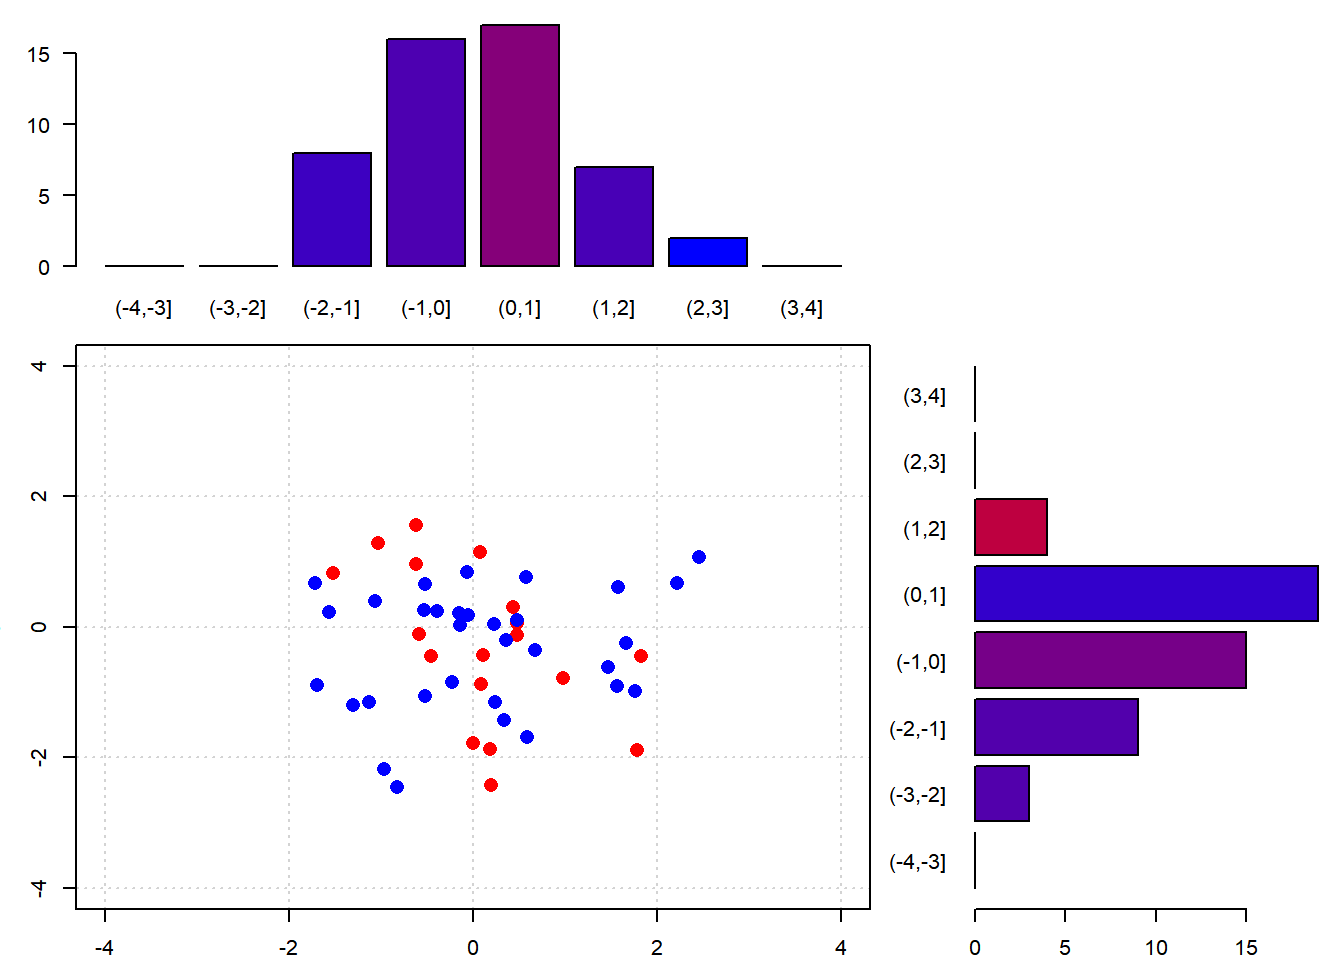
\includegraphics{myRBook_SP_files/figure-latex/unnamed-chunk-233-1.pdf}

\begin{Shaded}
\begin{Highlighting}[]
\KeywordTok{par}\NormalTok{(op)}
\end{Highlighting}
\end{Shaded}

La función \texttt{barplot()} también se puede usar para representar el
equivalente de un histograma. Esto puede ser útil para representar la
distribución de una variable en función del eje x el eje y. En el
siguiente ejemplo tenemos \texttt{n} puntos tomados aleatoriamente en
una distribución normal con la configuración \texttt{mean\ =\ 0} y
\texttt{sd\ =\ 1} (\texttt{myX\ \textless{}-\ rnorm(n)}). Estos puntos
son para ser mostrado en azul o en rojo (el color azul se codifica con
el valor 4 y el color rojo con el valor 2, discutiremos en un capítulo
posterior). La eleccion aleatoria del color se realiza con la función
\texttt{sample()}
(\texttt{myCol\ \textless{}-\ sample(c(4,\ 2),\ size\ =\ n,\ replace\ =\ TRUE)}).
Aquí queremos representar una nube de puntos con puntos rojos o azules,
y histogramas de los ejes X y Y para ver la distribución de puntos (con
un degradado de color de azul a rojo dependiendo La proporción de puntos
de color en cada categoría con un degradado de color con 100 valores
entre azul y rojo ;
\texttt{Mycolors\ \textless{}-\ colorRampPalette\ (c("azul",\ "rojo"))(100)}).

Para hacer el histograma, cortaremos los datos con la función
\texttt{cut()}, especificando que queremos que las separaciones se
realicen entre -4 y 4 en pasos de 1
(\texttt{myYCut\ \textless{}-\ cut(myY,\ breaks\ =\ -4:4)}). Para contar
el número de puntos en cada categoría y para cada color, solo usamos la
función \texttt{table()}
(\texttt{myYCutCol\ \textless{}-\ table(myCol,\ myYCut)}). En esta
tabla, la primera línea corresponde al primer color encontrado en el
conjunto de datos y la segunda línea al otro color. Es por eso que
necesitamos cambiar el dibujo aleatorio de los colores para que la
primera línea siempre corresponda a azul y la segunda línea a rojo:
\texttt{myCol\ \textless{}-\ c(2,\ sample(c(4,\ 2),\ size\ =\ (n\ -\ 1),\ replace\ =\ TRUE))}.

Luego podemos calcular la proporción de rojo dividiendo la primera línea
por la suma de las dos líneas que representaremos en porcentaje
multiplicando por 100:
\texttt{myXCutCol{[}1,{]}\ /\ (myXCutCol{[}1,{]}\ +\ myXCutCol{[}2,{]})\ *\ 100}.
Para que este número coincida con un color, solo mantendremos su parte
entera con la función \texttt{round()}. Si el porcentaje es cero o si el
resultado no es posible debido a una división por cero, debemos
reemplazarlo con 1 para que corresponda a un color en nuestro gradiente
que va de 1 a 100
(\texttt{xCol{[}is.na(xCol)\ \textbar{}\ xCol\ ==\ 0{]}\ \textless{}-\ 1}).

Todo lo que nos queda es organizar el espacio gráfico con la función
\texttt{layout()} que toma como argumento una matriz cuyos valores y su
posición corresponderán al diseño de los diferentes gráficos que
queremos lograr. El gráfico 1 corresponde al gráfico de barras superior,
el gráfico 2 a la nube de puntos y el gráfico 3 al gráfico de barras
derecho.

\begin{Shaded}
\begin{Highlighting}[]
\NormalTok{n <-}\StringTok{ }\DecValTok{50}
\NormalTok{myX <-}\StringTok{ }\KeywordTok{rnorm}\NormalTok{(n)}
\NormalTok{myY <-}\StringTok{ }\KeywordTok{rnorm}\NormalTok{(n)}
\NormalTok{myCol <-}\StringTok{ }\KeywordTok{c}\NormalTok{(}\DecValTok{2}\NormalTok{, }\KeywordTok{sample}\NormalTok{(}\KeywordTok{c}\NormalTok{(}\DecValTok{4}\NormalTok{, }\DecValTok{2}\NormalTok{), }\DataTypeTok{size =}\NormalTok{ (n }\OperatorTok{-}\StringTok{ }\DecValTok{1}\NormalTok{), }\DataTypeTok{replace =} \OtherTok{TRUE}\NormalTok{))}
\NormalTok{myColors <-}\StringTok{ }\KeywordTok{colorRampPalette}\NormalTok{(}\KeywordTok{c}\NormalTok{(}\StringTok{"blue"}\NormalTok{, }\StringTok{"red"}\NormalTok{))(}\DecValTok{100}\NormalTok{)}
\NormalTok{myYCut <-}\StringTok{ }\KeywordTok{cut}\NormalTok{(myY, }\DataTypeTok{breaks =} \OperatorTok{-}\DecValTok{4}\OperatorTok{:}\DecValTok{4}\NormalTok{)}
\NormalTok{myXCut <-}\StringTok{ }\KeywordTok{cut}\NormalTok{(myX, }\DataTypeTok{breaks =} \OperatorTok{-}\DecValTok{4}\OperatorTok{:}\DecValTok{4}\NormalTok{)}
\NormalTok{myYCutCol <-}\StringTok{ }\KeywordTok{table}\NormalTok{(myCol, myYCut)}
\NormalTok{myXCutCol <-}\StringTok{ }\KeywordTok{table}\NormalTok{(myCol, myXCut)}
\NormalTok{xCol <-}\StringTok{ }\KeywordTok{round}\NormalTok{(}
\NormalTok{  myXCutCol[}\DecValTok{1}\NormalTok{,] }\OperatorTok{/}\StringTok{ }\NormalTok{(myXCutCol[}\DecValTok{1}\NormalTok{,] }\OperatorTok{+}\StringTok{ }\NormalTok{myXCutCol[}\DecValTok{2}\NormalTok{,]) }\OperatorTok{*}\StringTok{ }\DecValTok{100}
\NormalTok{)}
\NormalTok{xCol[}\KeywordTok{is.na}\NormalTok{(xCol) }\OperatorTok{|}\StringTok{ }\NormalTok{xCol }\OperatorTok{==}\StringTok{ }\DecValTok{0}\NormalTok{] <-}\StringTok{ }\DecValTok{1}
\NormalTok{yCol <-}\StringTok{ }\KeywordTok{round}\NormalTok{(}
\NormalTok{  myYCutCol[}\DecValTok{1}\NormalTok{,] }\OperatorTok{/}\StringTok{ }\NormalTok{(myYCutCol[}\DecValTok{1}\NormalTok{,] }\OperatorTok{+}\StringTok{ }\NormalTok{myYCutCol[}\DecValTok{2}\NormalTok{,]) }\OperatorTok{*}\StringTok{ }\DecValTok{100}
\NormalTok{)}
\NormalTok{yCol[}\KeywordTok{is.na}\NormalTok{(yCol) }\OperatorTok{|}\StringTok{ }\NormalTok{yCol }\OperatorTok{==}\StringTok{ }\DecValTok{0}\NormalTok{] <-}\StringTok{ }\DecValTok{1}
\NormalTok{op <-}\StringTok{ }\KeywordTok{par}\NormalTok{(}\DataTypeTok{no.readonly =} \OtherTok{TRUE}\NormalTok{)}
\KeywordTok{par}\NormalTok{(}\DataTypeTok{mar =} \KeywordTok{c}\NormalTok{(}\DecValTok{2}\NormalTok{, }\DecValTok{3}\NormalTok{, }\DecValTok{1}\NormalTok{, }\DecValTok{1}\NormalTok{))}
\KeywordTok{layout}\NormalTok{(}\KeywordTok{matrix}\NormalTok{(}\KeywordTok{c}\NormalTok{(}\DecValTok{1}\NormalTok{, }\DecValTok{1}\NormalTok{, }\DecValTok{0}\NormalTok{, }
                \DecValTok{2}\NormalTok{, }\DecValTok{2}\NormalTok{, }\DecValTok{3}\NormalTok{, }
                \DecValTok{2}\NormalTok{, }\DecValTok{2}\NormalTok{, }\DecValTok{3}\NormalTok{), }\DataTypeTok{ncol =} \DecValTok{3}\NormalTok{, }\DataTypeTok{byrow =} \OtherTok{TRUE}\NormalTok{))}
\KeywordTok{barplot}\NormalTok{(}\KeywordTok{table}\NormalTok{(myXCut), }\DataTypeTok{las =} \DecValTok{1}\NormalTok{, }\DataTypeTok{col =}\NormalTok{ myColors[xCol])}
\KeywordTok{plot}\NormalTok{(}\DataTypeTok{x =}\NormalTok{ myX, }\DataTypeTok{y =}\NormalTok{ myY, }\DataTypeTok{col =}\NormalTok{ myCol, }\DataTypeTok{pch =} \DecValTok{16}\NormalTok{, }
  \DataTypeTok{xlim =} \KeywordTok{c}\NormalTok{(}\OperatorTok{-}\DecValTok{4}\NormalTok{, }\DecValTok{4}\NormalTok{), }\DataTypeTok{ylim =} \KeywordTok{c}\NormalTok{(}\OperatorTok{-}\DecValTok{4}\NormalTok{, }\DecValTok{4}\NormalTok{), }\DataTypeTok{cex =} \FloatTok{1.5}\NormalTok{, }
  \DataTypeTok{panel.first =} \KeywordTok{grid}\NormalTok{())}
\KeywordTok{barplot}\NormalTok{(}\KeywordTok{table}\NormalTok{(myYCut), }\DataTypeTok{las =} \DecValTok{1}\NormalTok{, }\DataTypeTok{horiz =} \OtherTok{TRUE}\NormalTok{, }\DataTypeTok{col =}\NormalTok{ myColors[yCol])}
\end{Highlighting}
\end{Shaded}

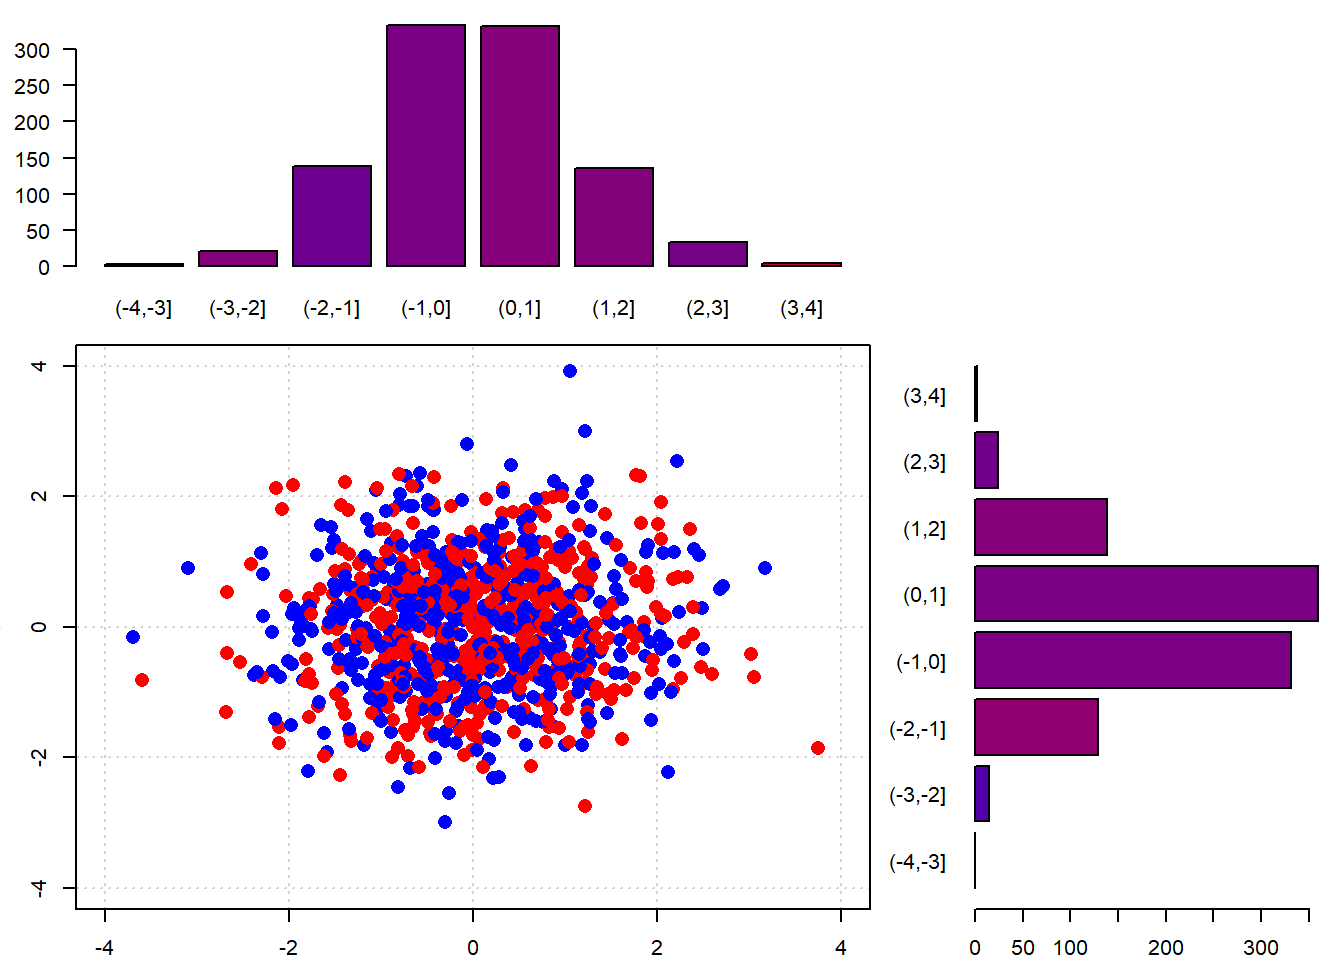
\includegraphics{myRBook_SP_files/figure-latex/unnamed-chunk-234-1.pdf}

\begin{Shaded}
\begin{Highlighting}[]
\KeywordTok{par}\NormalTok{(op)}
\end{Highlighting}
\end{Shaded}

Luego podemos integrar este script en una función para, por ejemplo,
estudiar el efecto de la variable \texttt{n}.

\begin{Shaded}
\begin{Highlighting}[]
\NormalTok{graphBarplotCol <-}\StringTok{ }\ControlFlowTok{function}\NormalTok{(n)\{}
\NormalTok{  myX <-}\StringTok{ }\KeywordTok{rnorm}\NormalTok{(n)}
\NormalTok{  myY <-}\StringTok{ }\KeywordTok{rnorm}\NormalTok{(n)}
\NormalTok{  myCol <-}\StringTok{ }\KeywordTok{c}\NormalTok{(}\DecValTok{2}\NormalTok{, }\KeywordTok{sample}\NormalTok{(}\KeywordTok{c}\NormalTok{(}\DecValTok{4}\NormalTok{, }\DecValTok{2}\NormalTok{), }\DataTypeTok{size =}\NormalTok{ (n }\OperatorTok{-}\StringTok{ }\DecValTok{1}\NormalTok{), }\DataTypeTok{replace =} \OtherTok{TRUE}\NormalTok{))}
\NormalTok{  myColors <-}\StringTok{ }\KeywordTok{colorRampPalette}\NormalTok{(}\KeywordTok{c}\NormalTok{(}\StringTok{"blue"}\NormalTok{, }\StringTok{"red"}\NormalTok{))(}\DecValTok{100}\NormalTok{)}
\NormalTok{  myYCut <-}\StringTok{ }\KeywordTok{cut}\NormalTok{(myY, }\DataTypeTok{breaks =} \OperatorTok{-}\DecValTok{4}\OperatorTok{:}\DecValTok{4}\NormalTok{)}
\NormalTok{  myXCut <-}\StringTok{ }\KeywordTok{cut}\NormalTok{(myX, }\DataTypeTok{breaks =} \OperatorTok{-}\DecValTok{4}\OperatorTok{:}\DecValTok{4}\NormalTok{)}
\NormalTok{  myYCutCol <-}\StringTok{ }\KeywordTok{table}\NormalTok{(myCol, myYCut)}
\NormalTok{  myXCutCol <-}\StringTok{ }\KeywordTok{table}\NormalTok{(myCol, myXCut)}
\NormalTok{  xCol <-}\StringTok{ }\KeywordTok{round}\NormalTok{(}
\NormalTok{    myXCutCol[}\DecValTok{1}\NormalTok{,] }\OperatorTok{/}\StringTok{ }\NormalTok{(myXCutCol[}\DecValTok{1}\NormalTok{,] }\OperatorTok{+}\StringTok{ }\NormalTok{myXCutCol[}\DecValTok{2}\NormalTok{,]) }\OperatorTok{*}\StringTok{ }\DecValTok{100}
\NormalTok{  )}
\NormalTok{  xCol[}\KeywordTok{is.na}\NormalTok{(xCol) }\OperatorTok{|}\StringTok{ }\NormalTok{xCol }\OperatorTok{==}\StringTok{ }\DecValTok{0}\NormalTok{] <-}\StringTok{ }\DecValTok{1}
\NormalTok{  yCol <-}\StringTok{ }\KeywordTok{round}\NormalTok{(}
\NormalTok{    myYCutCol[}\DecValTok{1}\NormalTok{,] }\OperatorTok{/}\StringTok{ }\NormalTok{(myYCutCol[}\DecValTok{1}\NormalTok{,] }\OperatorTok{+}\StringTok{ }\NormalTok{myYCutCol[}\DecValTok{2}\NormalTok{,]) }\OperatorTok{*}\StringTok{ }\DecValTok{100}
\NormalTok{  )}
\NormalTok{  yCol[}\KeywordTok{is.na}\NormalTok{(yCol) }\OperatorTok{|}\StringTok{ }\NormalTok{yCol }\OperatorTok{==}\StringTok{ }\DecValTok{0}\NormalTok{] <-}\StringTok{ }\DecValTok{1}
\NormalTok{  op <-}\StringTok{ }\KeywordTok{par}\NormalTok{(}\DataTypeTok{no.readonly =} \OtherTok{TRUE}\NormalTok{)}
  \KeywordTok{par}\NormalTok{(}\DataTypeTok{mar =} \KeywordTok{c}\NormalTok{(}\DecValTok{2}\NormalTok{, }\DecValTok{3}\NormalTok{, }\DecValTok{1}\NormalTok{, }\DecValTok{1}\NormalTok{))}
  \KeywordTok{layout}\NormalTok{(}\KeywordTok{matrix}\NormalTok{(}\KeywordTok{c}\NormalTok{(}\DecValTok{1}\NormalTok{, }\DecValTok{1}\NormalTok{, }\DecValTok{0}\NormalTok{, }
                  \DecValTok{2}\NormalTok{, }\DecValTok{2}\NormalTok{, }\DecValTok{3}\NormalTok{, }
                  \DecValTok{2}\NormalTok{, }\DecValTok{2}\NormalTok{, }\DecValTok{3}\NormalTok{), }\DataTypeTok{ncol =} \DecValTok{3}\NormalTok{, }\DataTypeTok{byrow =} \OtherTok{TRUE}\NormalTok{))}
  \KeywordTok{barplot}\NormalTok{(}\KeywordTok{table}\NormalTok{(myXCut), }\DataTypeTok{las =} \DecValTok{1}\NormalTok{, }\DataTypeTok{col =}\NormalTok{ myColors[xCol])}
  \KeywordTok{plot}\NormalTok{(}\DataTypeTok{x =}\NormalTok{ myX, }\DataTypeTok{y =}\NormalTok{ myY, }\DataTypeTok{col =}\NormalTok{ myCol, }\DataTypeTok{pch =} \DecValTok{16}\NormalTok{, }
    \DataTypeTok{xlim =} \KeywordTok{c}\NormalTok{(}\OperatorTok{-}\DecValTok{4}\NormalTok{, }\DecValTok{4}\NormalTok{), }\DataTypeTok{ylim =} \KeywordTok{c}\NormalTok{(}\OperatorTok{-}\DecValTok{4}\NormalTok{, }\DecValTok{4}\NormalTok{), }\DataTypeTok{cex =} \FloatTok{1.5}\NormalTok{, }
    \DataTypeTok{panel.first =} \KeywordTok{grid}\NormalTok{())}
  \KeywordTok{barplot}\NormalTok{(}\KeywordTok{table}\NormalTok{(myYCut), }\DataTypeTok{las =} \DecValTok{1}\NormalTok{, }\DataTypeTok{horiz =} \OtherTok{TRUE}\NormalTok{, }\DataTypeTok{col =}\NormalTok{ myColors[yCol])}
  \KeywordTok{par}\NormalTok{(op)}
\NormalTok{\}}
\KeywordTok{graphBarplotCol}\NormalTok{(}\DataTypeTok{n =} \DecValTok{1000}\NormalTok{)}
\end{Highlighting}
\end{Shaded}

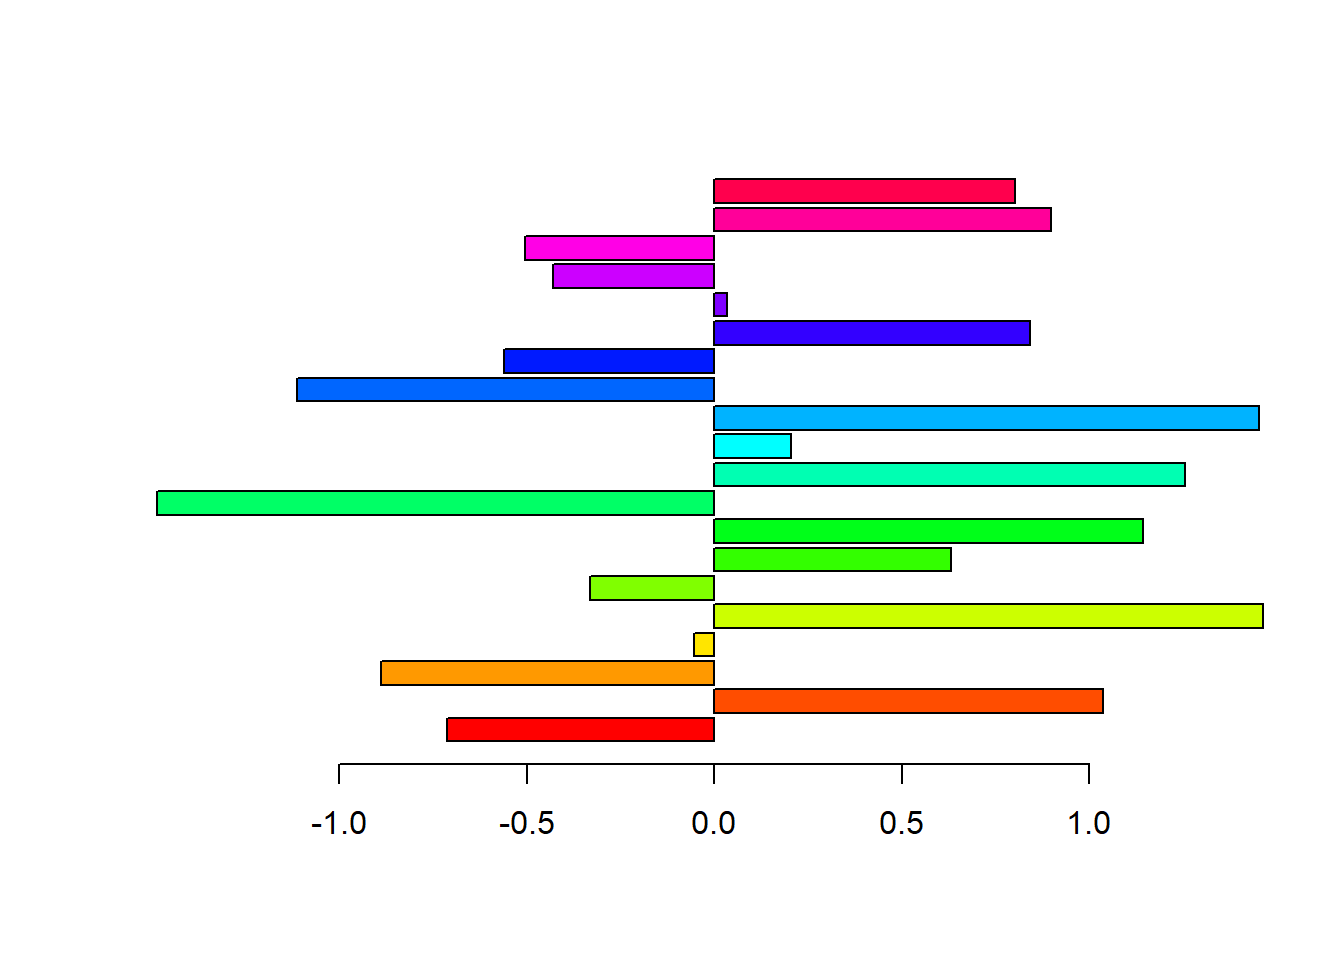
\includegraphics{myRBook_SP_files/figure-latex/unnamed-chunk-235-1.pdf}

Por supuesto, un \texttt{barplot} puede tomar valores positivos o
negativos.

\begin{Shaded}
\begin{Highlighting}[]
\KeywordTok{barplot}\NormalTok{(}\KeywordTok{rnorm}\NormalTok{(}\DecValTok{20}\NormalTok{), }\DataTypeTok{horiz =} \OtherTok{TRUE}\NormalTok{, }\DataTypeTok{col =} \KeywordTok{rainbow}\NormalTok{(}\DecValTok{20}\NormalTok{))}
\end{Highlighting}
\end{Shaded}

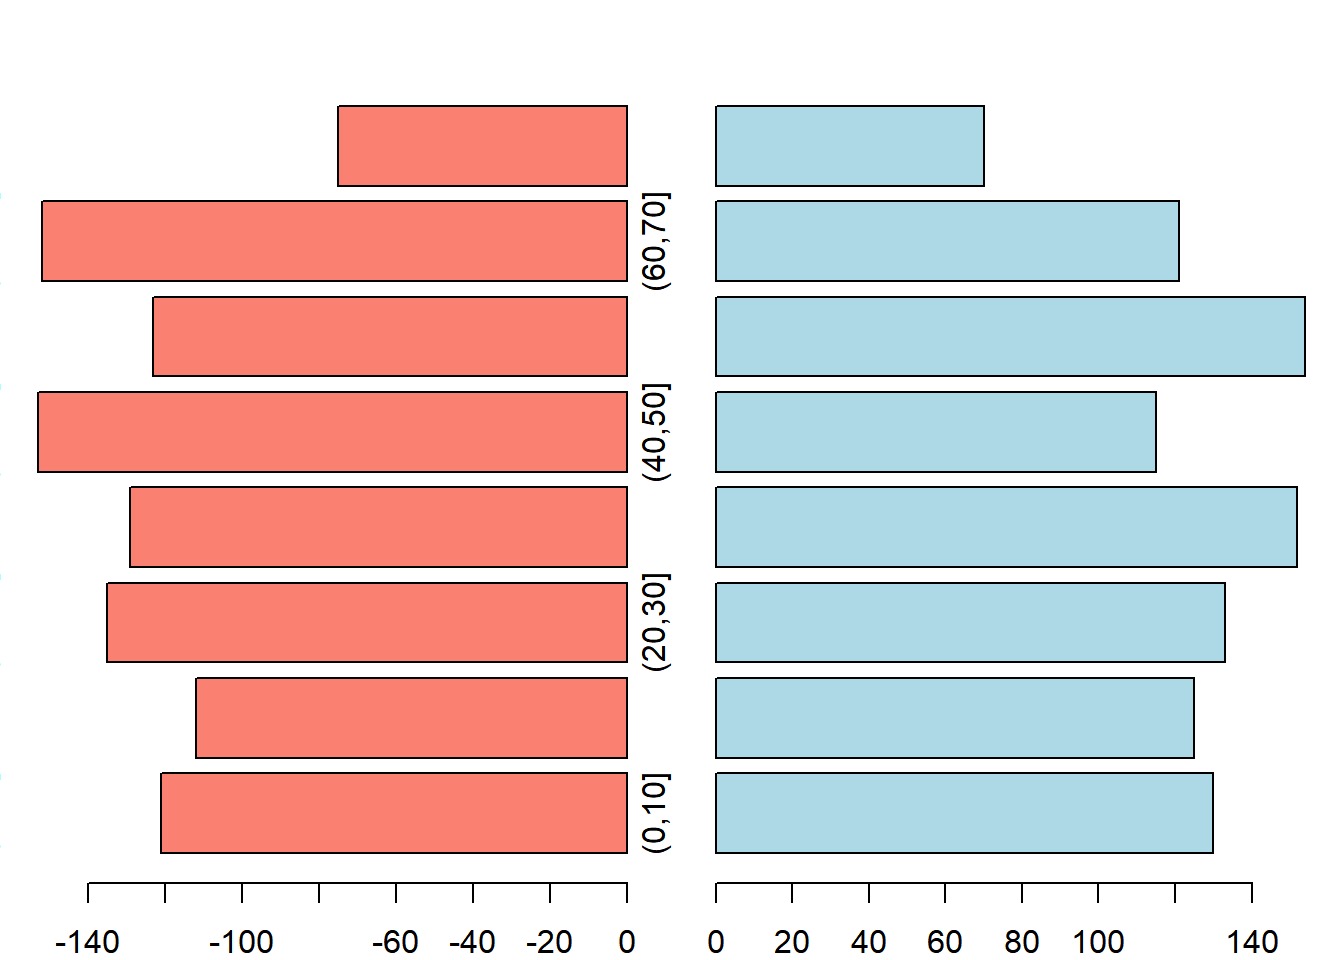
\includegraphics{myRBook_SP_files/figure-latex/unnamed-chunk-236-1.pdf}

El \texttt{barplot} también se puede usar para hacer una pirámide de
edades (hay funciones para realizar las las pirámides de edades, aquí el
objetivo es educativo).

\begin{Shaded}
\begin{Highlighting}[]
\NormalTok{gender <-}\StringTok{ }\KeywordTok{data.frame}\NormalTok{(}
  \DataTypeTok{m =} \KeywordTok{cut}\NormalTok{(}\KeywordTok{sample}\NormalTok{(}\DecValTok{1}\OperatorTok{:}\DecValTok{75}\NormalTok{, }\DecValTok{1000}\NormalTok{, }\DataTypeTok{replace =} \OtherTok{TRUE}\NormalTok{), }
    \DataTypeTok{breaks =} \KeywordTok{seq}\NormalTok{(}\DataTypeTok{from =} \DecValTok{0}\NormalTok{, }\DataTypeTok{to =} \DecValTok{80}\NormalTok{, }\DataTypeTok{by =} \DecValTok{10}\NormalTok{)), }
  \DataTypeTok{f =} \KeywordTok{cut}\NormalTok{(}\KeywordTok{sample}\NormalTok{(}\DecValTok{1}\OperatorTok{:}\DecValTok{75}\NormalTok{, }\DecValTok{1000}\NormalTok{, }\DataTypeTok{replace =} \OtherTok{TRUE}\NormalTok{), }
    \DataTypeTok{breaks =} \KeywordTok{seq}\NormalTok{(}\DataTypeTok{from =} \DecValTok{0}\NormalTok{, }\DataTypeTok{to =} \DecValTok{80}\NormalTok{, }\DataTypeTok{by =} \DecValTok{10}\NormalTok{))}
\NormalTok{)}
\NormalTok{op <-}\StringTok{ }\KeywordTok{par}\NormalTok{(}\DataTypeTok{no.readonly =} \OtherTok{TRUE}\NormalTok{)}
\KeywordTok{par}\NormalTok{(}\DataTypeTok{mfrow =} \KeywordTok{c}\NormalTok{(}\DecValTok{1}\NormalTok{, }\DecValTok{2}\NormalTok{), }\DataTypeTok{mar =} \KeywordTok{c}\NormalTok{(}\DecValTok{2}\NormalTok{, }\DecValTok{1}\NormalTok{, }\DecValTok{2}\NormalTok{, }\DecValTok{1}\NormalTok{))}
\KeywordTok{barplot}\NormalTok{(}\OperatorTok{-}\KeywordTok{table}\NormalTok{(gender}\OperatorTok{$}\NormalTok{f), }\DataTypeTok{horiz =} \OtherTok{TRUE}\NormalTok{, }\DataTypeTok{col =} \StringTok{"salmon"}\NormalTok{)}
\KeywordTok{barplot}\NormalTok{(}\KeywordTok{table}\NormalTok{(gender}\OperatorTok{$}\NormalTok{m), }\DataTypeTok{horiz =} \OtherTok{TRUE}\NormalTok{, }\DataTypeTok{col =} \StringTok{"lightblue"}\NormalTok{)}
\end{Highlighting}
\end{Shaded}

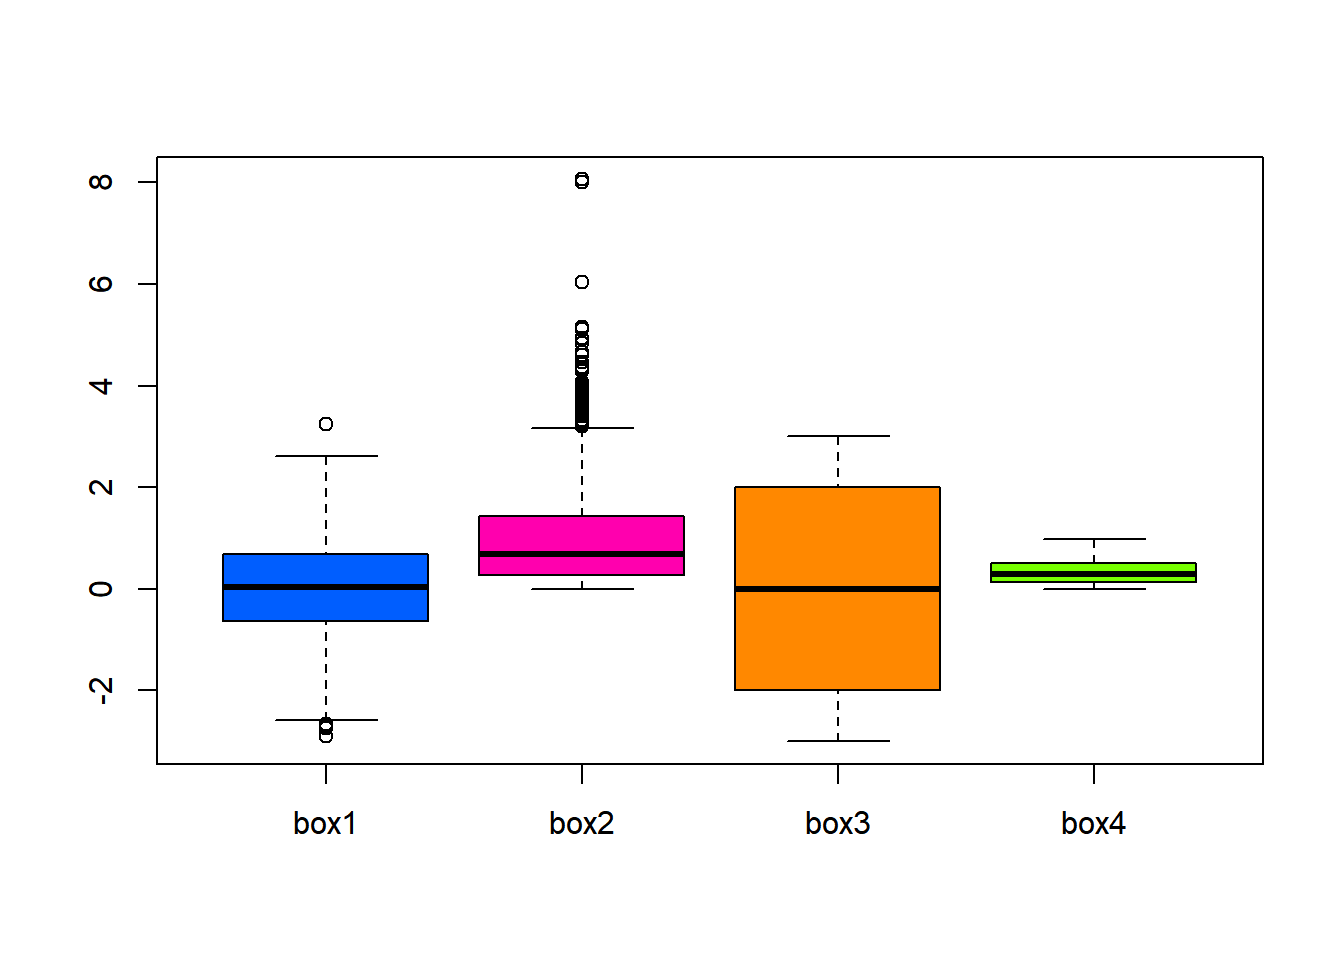
\includegraphics{myRBook_SP_files/figure-latex/unnamed-chunk-237-1.pdf}

\begin{Shaded}
\begin{Highlighting}[]
\KeywordTok{par}\NormalTok{(op)}
\end{Highlighting}
\end{Shaded}

\section{\texorpdfstring{\texttt{boxplot}}{boxplot}}\label{graph1boxplot}

Los diagramas de caja son gráficos muy comunes con R porque ofrecen una
buena vista de un conjunto de datos al representar los valores extremos
(valores atípicos), la mediana, los cuartiles, los mínimos y los
máximos.

La función \texttt{boxplot()} se aplica a uno o más \texttt{vector}.

\begin{Shaded}
\begin{Highlighting}[]
\NormalTok{df <-}\StringTok{ }\KeywordTok{data.frame}\NormalTok{(}
  \DataTypeTok{box1 =} \KeywordTok{rnorm}\NormalTok{(}\DecValTok{1000}\NormalTok{), }
  \DataTypeTok{box2 =} \KeywordTok{rgamma}\NormalTok{(}\DecValTok{1000}\NormalTok{, }\DataTypeTok{shape =} \DecValTok{1}\NormalTok{), }
  \DataTypeTok{box3 =} \KeywordTok{sample}\NormalTok{(}\OperatorTok{-}\DecValTok{3}\OperatorTok{:}\DecValTok{3}\NormalTok{, }\DataTypeTok{size =} \DecValTok{1000}\NormalTok{, }\DataTypeTok{replace =} \OtherTok{TRUE}\NormalTok{),}
  \DataTypeTok{box4 =} \KeywordTok{rbeta}\NormalTok{(}\DecValTok{1000}\NormalTok{, }\DataTypeTok{shape1 =} \DecValTok{1}\NormalTok{, }\DataTypeTok{shape2 =} \DecValTok{2}\NormalTok{)}
\NormalTok{)}
\KeywordTok{boxplot}\NormalTok{(df, }\DataTypeTok{col =} \KeywordTok{c}\NormalTok{(}\KeywordTok{rgb}\NormalTok{(}\DecValTok{0}\NormalTok{, }\DecValTok{94}\NormalTok{, }\DecValTok{255}\NormalTok{, }\DataTypeTok{maxColorValue =} \DecValTok{255}\NormalTok{),  }
  \KeywordTok{rgb}\NormalTok{(}\DecValTok{255}\NormalTok{, }\DecValTok{0}\NormalTok{, }\DecValTok{174}\NormalTok{, }\DataTypeTok{maxColorValue =} \DecValTok{255}\NormalTok{),  }
  \KeywordTok{rgb}\NormalTok{(}\DecValTok{255}\NormalTok{, }\DecValTok{136}\NormalTok{, }\DecValTok{0}\NormalTok{, }\DataTypeTok{maxColorValue =} \DecValTok{255}\NormalTok{),  }
  \KeywordTok{rgb}\NormalTok{(}\DecValTok{119}\NormalTok{, }\DecValTok{255}\NormalTok{, }\DecValTok{0}\NormalTok{, }\DataTypeTok{maxColorValue =} \DecValTok{255}\NormalTok{)))}
\end{Highlighting}
\end{Shaded}

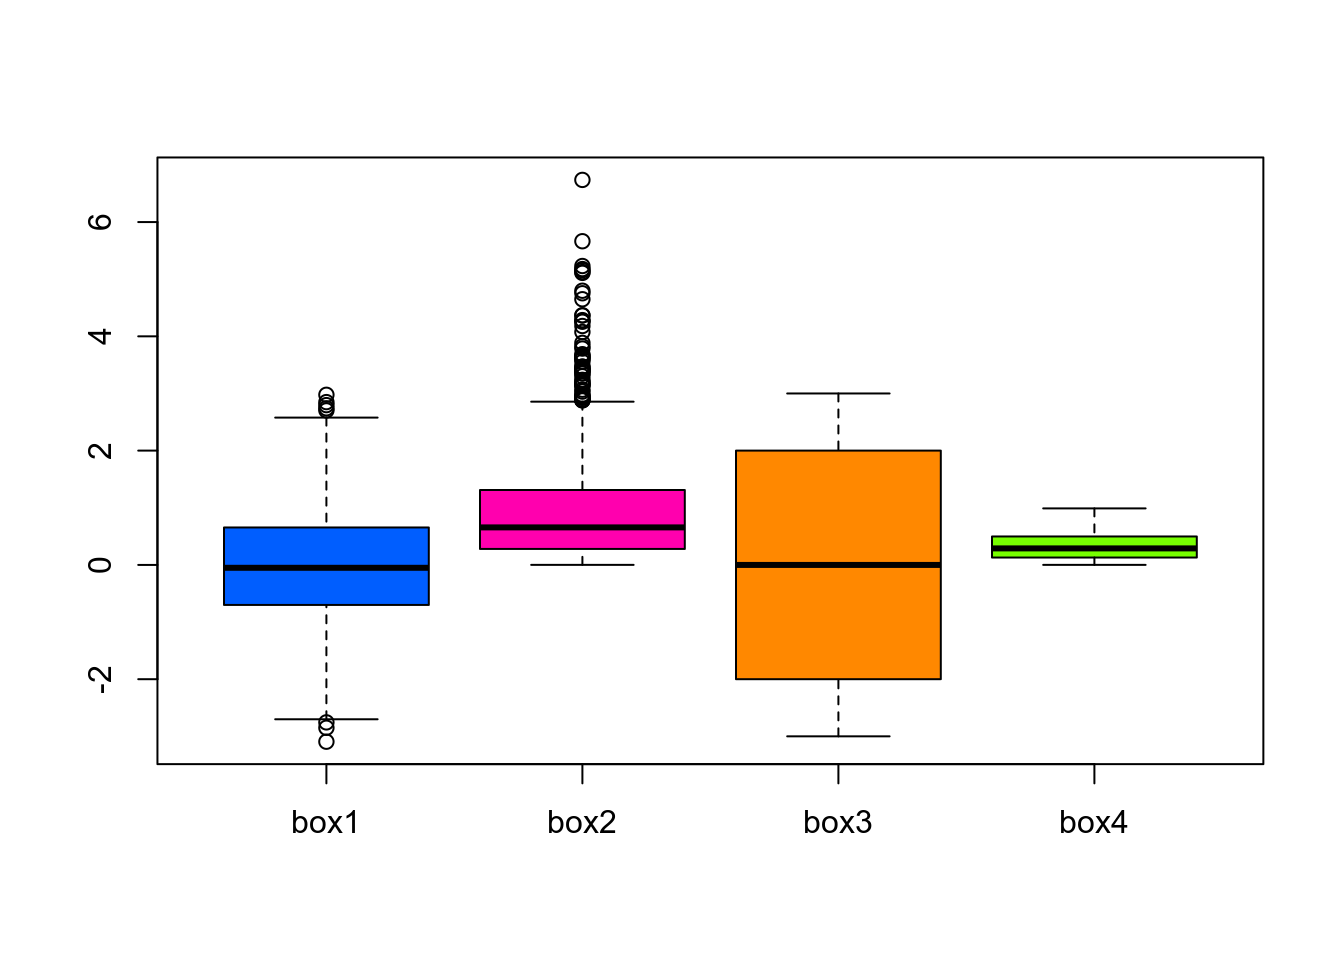
\includegraphics{myRBook_SP_files/figure-latex/unnamed-chunk-238-1.pdf}

Si una variable es de tipo \texttt{factor}, la función
\texttt{boxplot()} facilita la representación de cada categoría. También
funciona con variables numéricas, pero se debe tener cuidado de no tener
demasiados valores diferentes para que el gráfico permanezca legible.

\begin{Shaded}
\begin{Highlighting}[]
\NormalTok{df}\OperatorTok{$}\NormalTok{cat <-}\StringTok{ }\KeywordTok{sample}\NormalTok{(}\KeywordTok{c}\NormalTok{(}\StringTok{"w"}\NormalTok{, }\StringTok{"x"}\NormalTok{, }\StringTok{"y"}\NormalTok{, }\StringTok{"z"}\NormalTok{), }\DataTypeTok{size =} \DecValTok{1000}\NormalTok{, }\DataTypeTok{replace =} \OtherTok{TRUE}\NormalTok{)}
\KeywordTok{boxplot}\NormalTok{(df}\OperatorTok{$}\NormalTok{box3 }\OperatorTok{~}\StringTok{ }\NormalTok{df}\OperatorTok{$}\NormalTok{cat, }\DataTypeTok{col =} \KeywordTok{c}\NormalTok{(}\KeywordTok{rgb}\NormalTok{(}\DecValTok{0}\NormalTok{, }\DecValTok{94}\NormalTok{, }\DecValTok{255}\NormalTok{, }\DataTypeTok{maxColorValue =} \DecValTok{255}\NormalTok{),  }
  \KeywordTok{rgb}\NormalTok{(}\DecValTok{255}\NormalTok{, }\DecValTok{0}\NormalTok{, }\DecValTok{174}\NormalTok{, }\DataTypeTok{maxColorValue =} \DecValTok{255}\NormalTok{),  }
  \KeywordTok{rgb}\NormalTok{(}\DecValTok{255}\NormalTok{, }\DecValTok{136}\NormalTok{, }\DecValTok{0}\NormalTok{, }\DataTypeTok{maxColorValue =} \DecValTok{255}\NormalTok{),  }
  \KeywordTok{rgb}\NormalTok{(}\DecValTok{119}\NormalTok{, }\DecValTok{255}\NormalTok{, }\DecValTok{0}\NormalTok{, }\DataTypeTok{maxColorValue =} \DecValTok{255}\NormalTok{)), }\DataTypeTok{ylab =} \StringTok{"Box3"}\NormalTok{)}
\end{Highlighting}
\end{Shaded}

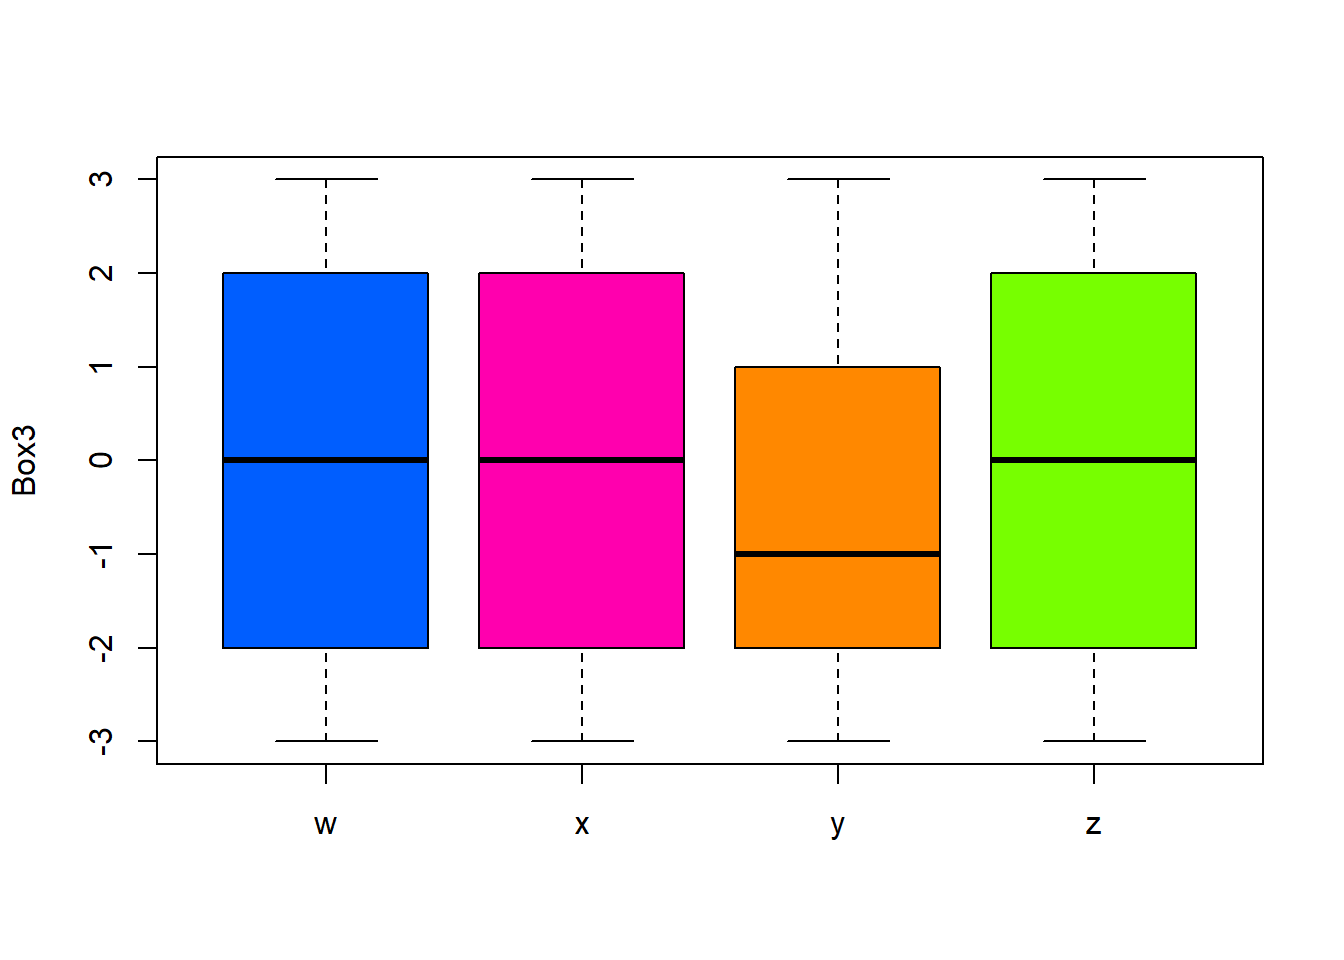
\includegraphics{myRBook_SP_files/figure-latex/unnamed-chunk-239-1.pdf}

\begin{Shaded}
\begin{Highlighting}[]
\NormalTok{df}\OperatorTok{$}\NormalTok{cat2 <-}\StringTok{ }\KeywordTok{sample}\NormalTok{(}\DecValTok{1}\OperatorTok{:}\DecValTok{3}\NormalTok{, }\DataTypeTok{size =} \DecValTok{1000}\NormalTok{, }\DataTypeTok{replace =} \OtherTok{TRUE}\NormalTok{)}
\KeywordTok{boxplot}\NormalTok{(df}\OperatorTok{$}\NormalTok{box4 }\OperatorTok{~}\StringTok{ }\NormalTok{df}\OperatorTok{$}\NormalTok{cat}\OperatorTok{*}\NormalTok{df}\OperatorTok{$}\NormalTok{cat2, }\DataTypeTok{col =} \KeywordTok{c}\NormalTok{(}
  \KeywordTok{rgb}\NormalTok{(}\DecValTok{0}\NormalTok{, }\DecValTok{94}\NormalTok{, }\DecValTok{255}\NormalTok{, }\DataTypeTok{maxColorValue =} \DecValTok{255}\NormalTok{),  }
  \KeywordTok{rgb}\NormalTok{(}\DecValTok{255}\NormalTok{, }\DecValTok{0}\NormalTok{, }\DecValTok{174}\NormalTok{, }\DataTypeTok{maxColorValue =} \DecValTok{255}\NormalTok{),  }
  \KeywordTok{rgb}\NormalTok{(}\DecValTok{255}\NormalTok{, }\DecValTok{136}\NormalTok{, }\DecValTok{0}\NormalTok{, }\DataTypeTok{maxColorValue =} \DecValTok{255}\NormalTok{),  }
  \KeywordTok{rgb}\NormalTok{(}\DecValTok{119}\NormalTok{, }\DecValTok{255}\NormalTok{, }\DecValTok{0}\NormalTok{, }\DataTypeTok{maxColorValue =} \DecValTok{255}\NormalTok{)), }\DataTypeTok{ylab =} \StringTok{"Box4"}\NormalTok{)}
\end{Highlighting}
\end{Shaded}

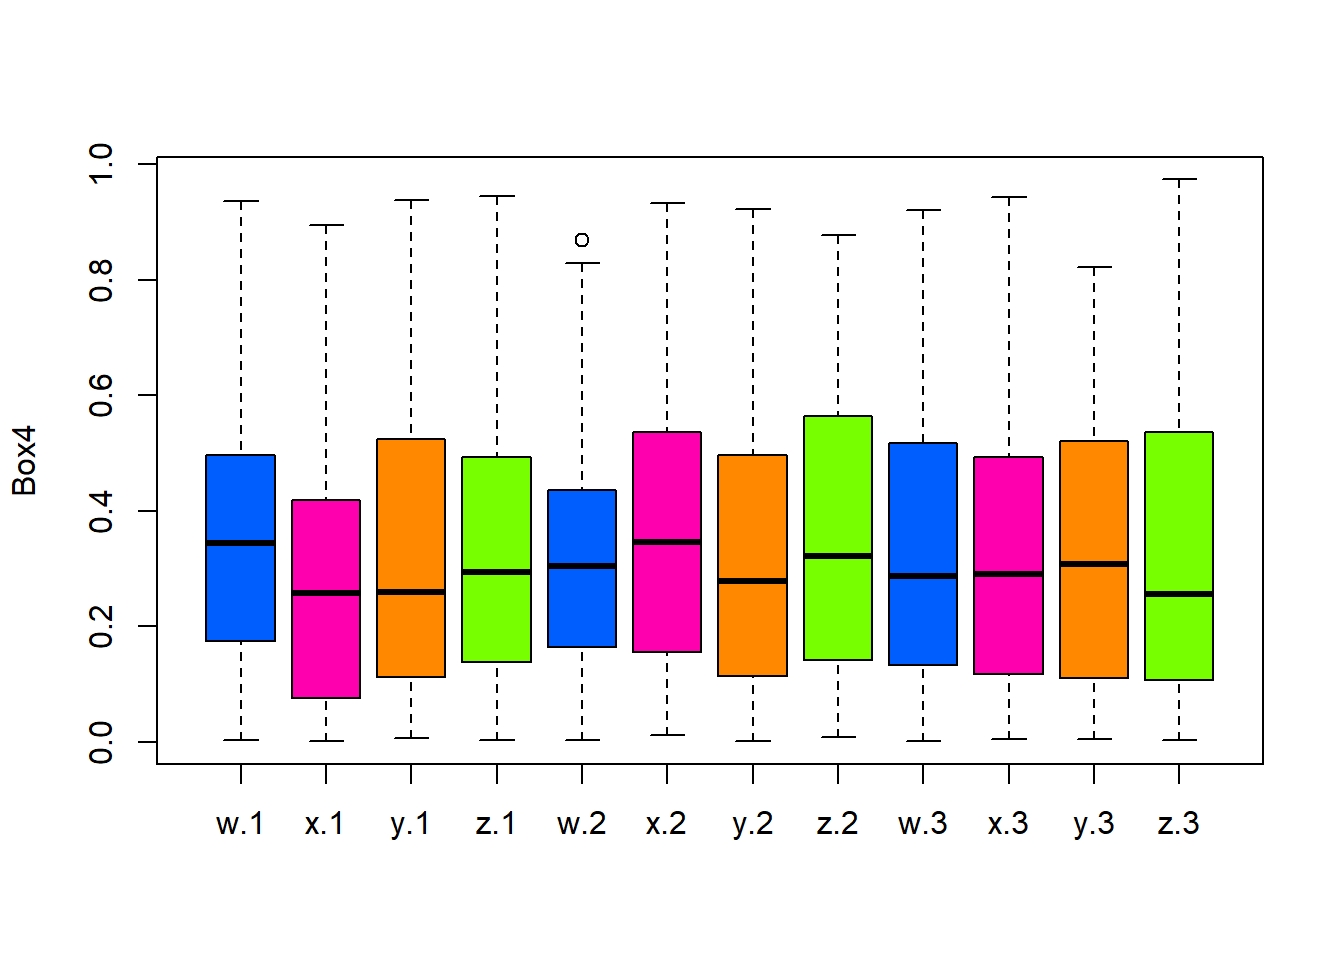
\includegraphics{myRBook_SP_files/figure-latex/unnamed-chunk-239-2.pdf}

El \texttt{boxplot} puede representarse horizontal o verticalmente.

\begin{Shaded}
\begin{Highlighting}[]
\NormalTok{df}\OperatorTok{$}\NormalTok{cat <-}\StringTok{ }\KeywordTok{sample}\NormalTok{(}\KeywordTok{c}\NormalTok{(}\StringTok{"w"}\NormalTok{, }\StringTok{"x"}\NormalTok{, }\StringTok{"y"}\NormalTok{, }\StringTok{"z"}\NormalTok{), }\DataTypeTok{size =} \DecValTok{1000}\NormalTok{, }\DataTypeTok{replace =} \OtherTok{TRUE}\NormalTok{)}
\KeywordTok{boxplot}\NormalTok{(df}\OperatorTok{$}\NormalTok{box2 }\OperatorTok{~}\StringTok{ }\NormalTok{df}\OperatorTok{$}\NormalTok{cat, }\DataTypeTok{horizontal =} \OtherTok{TRUE}\NormalTok{, }
  \DataTypeTok{col =} \KeywordTok{c}\NormalTok{(}\KeywordTok{rgb}\NormalTok{(}\DecValTok{255}\NormalTok{, }\DecValTok{110}\NormalTok{, }\DecValTok{0}\NormalTok{, }\DataTypeTok{maxColorValue =} \DecValTok{255}\NormalTok{),  }
  \KeywordTok{rgb}\NormalTok{(}\DecValTok{230}\NormalTok{, }\DecValTok{255}\NormalTok{, }\DecValTok{0}\NormalTok{, }\DataTypeTok{maxColorValue =} \DecValTok{255}\NormalTok{),  }
  \KeywordTok{rgb}\NormalTok{(}\DecValTok{0}\NormalTok{, }\DecValTok{178}\NormalTok{, }\DecValTok{255}\NormalTok{, }\DataTypeTok{maxColorValue =} \DecValTok{255}\NormalTok{),  }
  \KeywordTok{rgb}\NormalTok{(}\DecValTok{166}\NormalTok{, }\DecValTok{0}\NormalTok{, }\DecValTok{255}\NormalTok{, }\DataTypeTok{maxColorValue =} \DecValTok{255}\NormalTok{)), }\DataTypeTok{xlab =} \StringTok{"Box2"}\NormalTok{)}
\end{Highlighting}
\end{Shaded}

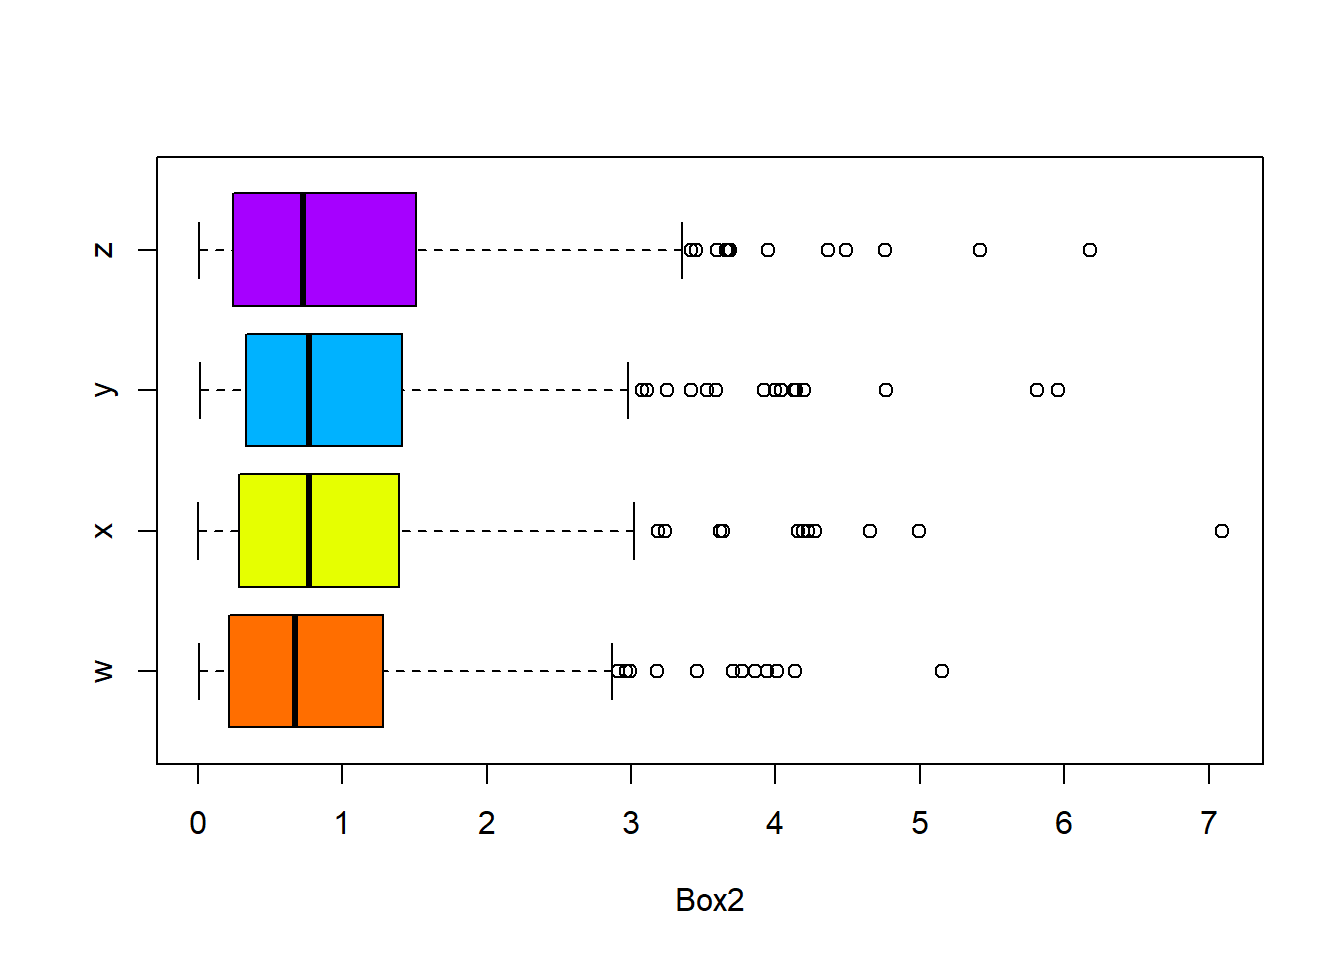
\includegraphics{myRBook_SP_files/figure-latex/unnamed-chunk-240-1.pdf}

\section{Otros gráficos}\label{otros-graficos}

Hay muchos otros gráficos, pero los que acabamos de ver son la base.
Para obtener más información e ideas para representar sus datos, podemos
consultar el hermoso sitio \url{https://www.data-to-viz.com/} o la
galería gráfica R \url{https://www.r-graph-gallery.com/} (la mayoría de
los gráficos se realizan con el paquete ggplot2 que veremos más
adelante). Para obtener más ideas, también podemos usar la demostración
del paquete \texttt{graphics} usando el comando
\texttt{demo(\textquotesingle{}graphics\textquotesingle{})} (la tecla
``Enter'' se usa para mostrar los gráficos).

\section{Conclusión}\label{conclusion-8}

Felicitaciones, hemos llegado al final de este capítulo sobre gráficos
simples. Ahora sabemos cómo hacer que los gráficos principales
\texttt{plot()}, \texttt{hist()}, \texttt{barplot()}, y
\texttt{boxplot()}. A lo largo de este capítulo, hemos utilizado
diferentes colores y diferentes formas de representar los colores: es
hora de formalizar el uso y la gestión de los colores. ¡Este es el tema
del próximo capítulo!

\hypertarget{graph2}{\chapter{Gestión del color}\label{graph2}}

Hemos visto diferentes formas de usar los colores: con su nombre (por
ejemplo, \texttt{"salmón"}), con un número del 1 al 8, con la función
\texttt{rgb()} (para ``rojo / red'', ``verde / green'', ``azul /
blue''), y con la función \texttt{colors()}. Hay otros pero estos son
los principales.

El uso de los números del 1 al 8 corresponde a negro, rojo, verde, azul,
cian, magenta, amarillo y gris. Este uso es útil para visualizar
rápidamente nuestros resultados, pero proporciona gráficos generales
visualmente promedio. Es preferable evitar estos colores para comunicar
nuestros gráficos o para construir figuras en revistas científicas.

\begin{Shaded}
\begin{Highlighting}[]
\KeywordTok{barplot}\NormalTok{(}\KeywordTok{sample}\NormalTok{(}\DecValTok{10}\OperatorTok{:}\DecValTok{15}\NormalTok{, }\DecValTok{8}\NormalTok{, }\DataTypeTok{replace =} \OtherTok{TRUE}\NormalTok{), }\DataTypeTok{col =} \DecValTok{1}\OperatorTok{:}\DecValTok{8}\NormalTok{, }\DataTypeTok{names.arg =} \DecValTok{1}\OperatorTok{:}\DecValTok{8}\NormalTok{)}
\end{Highlighting}
\end{Shaded}

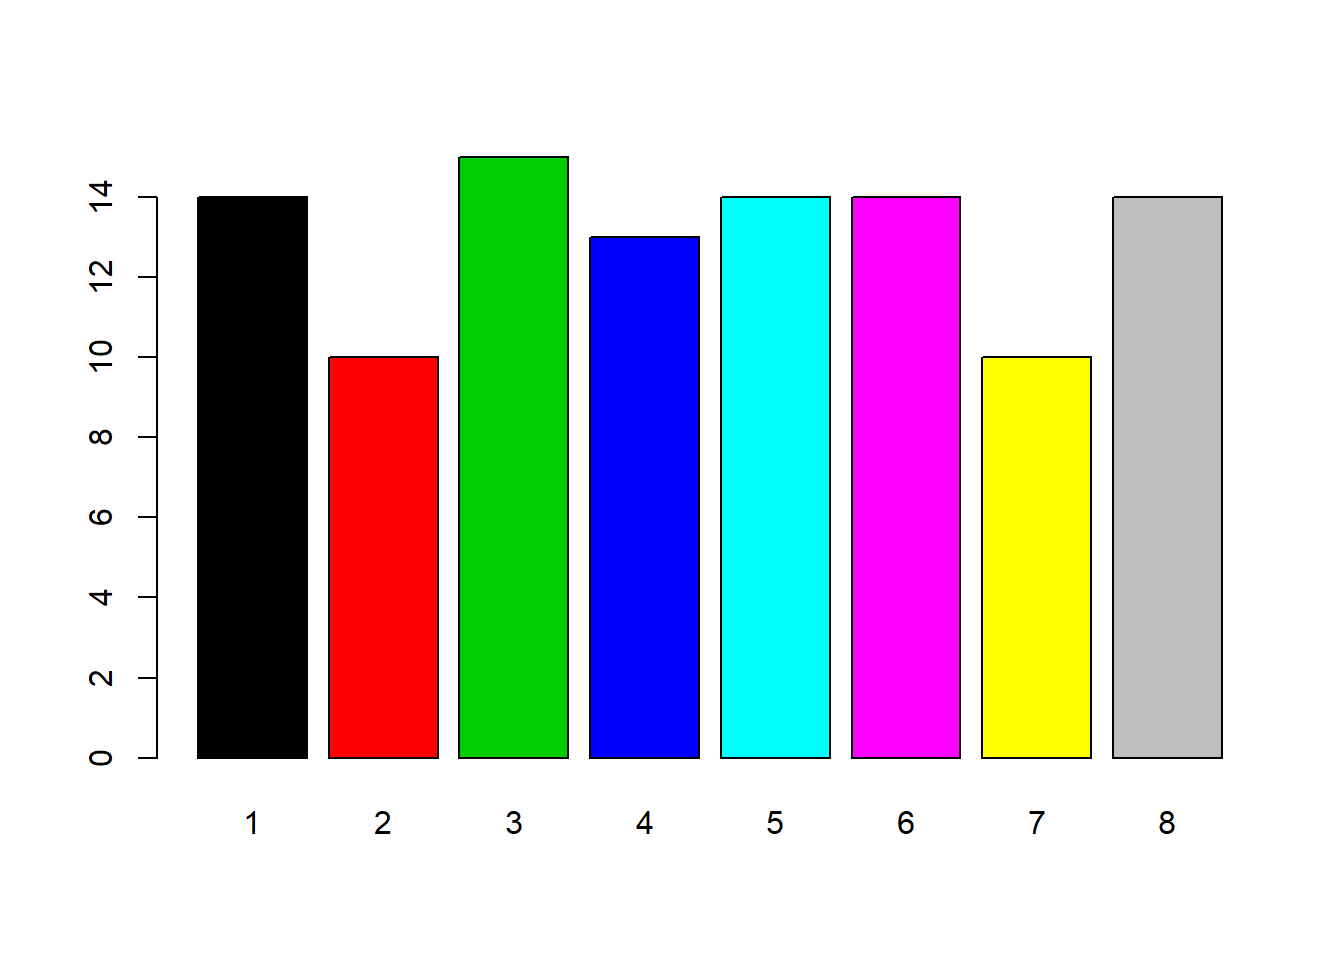
\includegraphics{myRBook_SP_files/figure-latex/unnamed-chunk-241-1.pdf}

\section{\texorpdfstring{\texttt{colors()}}{colors()}}\label{colors}

Para elegir colores más agradables y resaltar nuestros resultados, una
opción es elegir de la lista de colores pregrabados en R. Podemos
acceder a la lista de colores con la función \texttt{colors()}

\begin{Shaded}
\begin{Highlighting}[]
\KeywordTok{head}\NormalTok{(}\KeywordTok{colors}\NormalTok{(), }\DataTypeTok{n =} \DecValTok{20}\NormalTok{)}
\end{Highlighting}
\end{Shaded}

\begin{verbatim}
##  [1] "white"         "aliceblue"     "antiquewhite"  "antiquewhite1"
##  [5] "antiquewhite2" "antiquewhite3" "antiquewhite4" "aquamarine"   
##  [9] "aquamarine1"   "aquamarine2"   "aquamarine3"   "aquamarine4"  
## [13] "azure"         "azure1"        "azure2"        "azure3"       
## [17] "azure4"        "beige"         "bisque"        "bisque1"
\end{verbatim}

Podemos usar estos colores con sus nombres (por ejemplo,
\texttt{"white"}, \texttt{"azure3"}), o con su número (por ejemplo,
``white'' = \texttt{colors(){[}1{]}}, ``azure3'' =
\texttt{colors(){[}16{]}}).

\begin{Shaded}
\begin{Highlighting}[]
\CommentTok{# adapted from http://www.r-graph-gallery.com/42-colors-names/}
\NormalTok{op <-}\StringTok{ }\KeywordTok{par}\NormalTok{(}\DataTypeTok{no.readonly =} \OtherTok{TRUE}\NormalTok{)}
\KeywordTok{par}\NormalTok{(}\DataTypeTok{mar =} \KeywordTok{c}\NormalTok{(}\DecValTok{0}\NormalTok{, }\DecValTok{0}\NormalTok{, }\DecValTok{0}\NormalTok{, }\DecValTok{0}\NormalTok{))}
\KeywordTok{plot}\NormalTok{(}\DecValTok{0}\NormalTok{, }\DataTypeTok{type =} \StringTok{"n"}\NormalTok{, }\DataTypeTok{xlim =} \KeywordTok{c}\NormalTok{(}\DecValTok{0}\NormalTok{, }\DecValTok{1}\NormalTok{), }\DataTypeTok{ylim =} \KeywordTok{c}\NormalTok{(}\DecValTok{0}\NormalTok{, }\DecValTok{1}\NormalTok{), }
  \DataTypeTok{axes =} \OtherTok{FALSE}\NormalTok{, }\DataTypeTok{xlab =} \StringTok{""}\NormalTok{, }\DataTypeTok{ylab =} \StringTok{""}\NormalTok{)}
\NormalTok{numRow <-}\StringTok{ }\DecValTok{26}
\NormalTok{numCol <-}\StringTok{ }\DecValTok{26}
\KeywordTok{rect}\NormalTok{(}
  \DataTypeTok{xleft =} \KeywordTok{rep}\NormalTok{((}\DecValTok{0}\OperatorTok{:}\NormalTok{(numCol }\OperatorTok{-}\StringTok{ }\DecValTok{1}\NormalTok{)}\OperatorTok{/}\NormalTok{numCol), numRow),  }
  \DataTypeTok{ybottom =} \KeywordTok{sort}\NormalTok{(}\KeywordTok{rep}\NormalTok{((}\DecValTok{0}\OperatorTok{:}\NormalTok{(numRow }\OperatorTok{-}\StringTok{ }\DecValTok{1}\NormalTok{)}\OperatorTok{/}\NormalTok{numRow),numCol), }\DataTypeTok{decreasing =} \OtherTok{TRUE}\NormalTok{),}
  \DataTypeTok{xright =} \KeywordTok{rep}\NormalTok{((}\DecValTok{1}\OperatorTok{:}\NormalTok{numCol}\OperatorTok{/}\NormalTok{numCol), numRow),}
  \DataTypeTok{ytop =} \KeywordTok{sort}\NormalTok{(}\KeywordTok{rep}\NormalTok{((}\DecValTok{1}\OperatorTok{:}\NormalTok{numRow}\OperatorTok{/}\NormalTok{numRow), numCol), }\DataTypeTok{decreasing =} \OtherTok{TRUE}\NormalTok{),}
  \DataTypeTok{border =} \KeywordTok{grey}\NormalTok{(}\FloatTok{0.5}\NormalTok{), }
  \DataTypeTok{col =} \KeywordTok{colors}\NormalTok{()[}\KeywordTok{seq}\NormalTok{(}\DecValTok{1}\NormalTok{, numRow}\OperatorTok{*}\NormalTok{numCol)])}
\NormalTok{myLabels <-}\StringTok{ }\KeywordTok{c}\NormalTok{(}\KeywordTok{as.character}\NormalTok{(}\DecValTok{1}\OperatorTok{:}\DecValTok{657}\NormalTok{), }\KeywordTok{rep}\NormalTok{(}\StringTok{""}\NormalTok{, numRow}\OperatorTok{*}\NormalTok{numCol }\OperatorTok{-}\StringTok{ }\DecValTok{657}\NormalTok{))}
\KeywordTok{text}\NormalTok{(}
  \DataTypeTok{x =} \KeywordTok{rep}\NormalTok{((}\DecValTok{0}\OperatorTok{:}\NormalTok{(numCol }\OperatorTok{-}\StringTok{ }\DecValTok{1}\NormalTok{)}\OperatorTok{/}\NormalTok{numCol), numRow) }\OperatorTok{+}\StringTok{ }\FloatTok{0.02}\NormalTok{,}
  \DataTypeTok{y =} \KeywordTok{sort}\NormalTok{(}\KeywordTok{rep}\NormalTok{((}\DecValTok{0}\OperatorTok{:}\NormalTok{(numRow }\OperatorTok{-}\StringTok{ }\DecValTok{1}\NormalTok{)}\OperatorTok{/}\NormalTok{numRow), numCol), }\DataTypeTok{decreasing =} \OtherTok{TRUE}\NormalTok{) }\OperatorTok{+}\StringTok{ }\FloatTok{0.02}\NormalTok{,}
  \DataTypeTok{labels =}\NormalTok{ myLabels, }
  \DataTypeTok{cex =} \FloatTok{0.6}\NormalTok{)}
\end{Highlighting}
\end{Shaded}

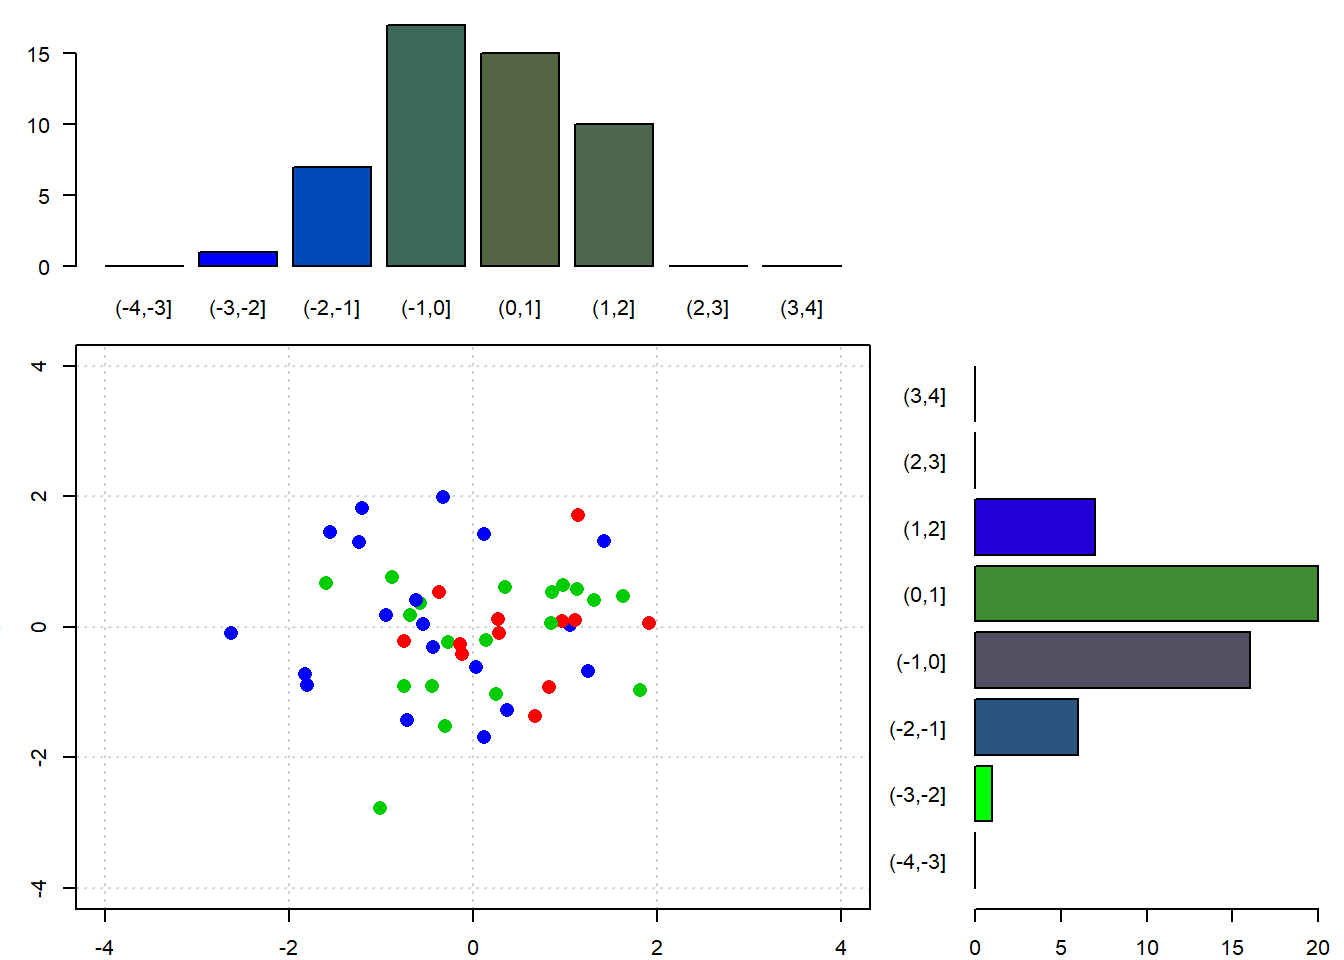
\includegraphics{myRBook_SP_files/figure-latex/unnamed-chunk-243-1.pdf}

\begin{Shaded}
\begin{Highlighting}[]
\KeywordTok{par}\NormalTok{(op)}
\end{Highlighting}
\end{Shaded}

\section{\texorpdfstring{\texttt{rgb()}}{rgb()}}\label{rgb}

Otra opción es crear nuestros propios colores con la función
\texttt{rgb()}, que toma la cantidad de rojo, verde y azul como
argumentos. De forma predeterminada, estos valores se encuentran entre 0
y 1. Esta configuración predeterminada se puede cambiar con el argumento
\texttt{maxColorValue} para, por ejemplo, tener valores entre 0 y 255
(\texttt{maxColorValue\ =\ 255}, estándar para la representación del
color RGB) .

Vamos a reanudar nuestra función para representar la distribución de
puntos en un diagrama de dispersión por medio de \texttt{barplot} con
este tiempo tres colores de puntos (rojo, verde, azul) y un
\texttt{barplot} cuyo color corresponderá a la cantidad de cada color
con la función \texttt{rgb()}.

\begin{Shaded}
\begin{Highlighting}[]
\NormalTok{graphBarplotCol <-}\StringTok{ }\ControlFlowTok{function}\NormalTok{(n)\{}
\NormalTok{  myX <-}\StringTok{ }\KeywordTok{rnorm}\NormalTok{(n)}
\NormalTok{  myY <-}\StringTok{ }\KeywordTok{rnorm}\NormalTok{(n)}
\NormalTok{  myCol <-}\StringTok{ }\KeywordTok{c}\NormalTok{(}\DecValTok{2}\NormalTok{, }\DecValTok{3}\NormalTok{, }\DecValTok{4}\NormalTok{, }\KeywordTok{sample}\NormalTok{(}\DecValTok{2}\OperatorTok{:}\DecValTok{4}\NormalTok{, }\DataTypeTok{size =}\NormalTok{ (n }\OperatorTok{-}\StringTok{ }\DecValTok{3}\NormalTok{), }\DataTypeTok{replace =} \OtherTok{TRUE}\NormalTok{))}
\NormalTok{  myYCut <-}\StringTok{ }\KeywordTok{cut}\NormalTok{(myY, }\DataTypeTok{breaks =} \OperatorTok{-}\DecValTok{4}\OperatorTok{:}\DecValTok{4}\NormalTok{)}
\NormalTok{  myXCut <-}\StringTok{ }\KeywordTok{cut}\NormalTok{(myX, }\DataTypeTok{breaks =} \OperatorTok{-}\DecValTok{4}\OperatorTok{:}\DecValTok{4}\NormalTok{)}
\NormalTok{  myYCutCol <-}\StringTok{ }\KeywordTok{table}\NormalTok{(myCol, myYCut)}
\NormalTok{  myXCutCol <-}\StringTok{ }\KeywordTok{table}\NormalTok{(myCol, myXCut)}
\NormalTok{  rColX <-}\StringTok{ }\NormalTok{myXCutCol[}\DecValTok{1}\NormalTok{,] }\OperatorTok{/}\StringTok{ }\NormalTok{(myXCutCol[}\DecValTok{1}\NormalTok{,] }\OperatorTok{+}\StringTok{ }\NormalTok{myXCutCol[}\DecValTok{2}\NormalTok{,] }\OperatorTok{+}\StringTok{ }
\StringTok{                              }\NormalTok{myXCutCol[}\DecValTok{3}\NormalTok{,])}
\NormalTok{  gColX <-}\StringTok{ }\NormalTok{myXCutCol[}\DecValTok{2}\NormalTok{,] }\OperatorTok{/}\StringTok{ }\NormalTok{(myXCutCol[}\DecValTok{1}\NormalTok{,] }\OperatorTok{+}\StringTok{ }\NormalTok{myXCutCol[}\DecValTok{2}\NormalTok{,] }\OperatorTok{+}\StringTok{ }
\StringTok{                              }\NormalTok{myXCutCol[}\DecValTok{3}\NormalTok{,])}
\NormalTok{  bColX <-}\StringTok{ }\NormalTok{myXCutCol[}\DecValTok{3}\NormalTok{,] }\OperatorTok{/}\StringTok{ }\NormalTok{(myXCutCol[}\DecValTok{1}\NormalTok{,] }\OperatorTok{+}\StringTok{ }\NormalTok{myXCutCol[}\DecValTok{2}\NormalTok{,] }\OperatorTok{+}\StringTok{ }
\StringTok{                              }\NormalTok{myXCutCol[}\DecValTok{3}\NormalTok{,])}
\NormalTok{  rColX[}\KeywordTok{is.na}\NormalTok{(rColX)] <-}\StringTok{ }\DecValTok{0}
\NormalTok{  gColX[}\KeywordTok{is.na}\NormalTok{(gColX)] <-}\StringTok{ }\DecValTok{0}
\NormalTok{  bColX[}\KeywordTok{is.na}\NormalTok{(bColX)] <-}\StringTok{ }\DecValTok{0}
\NormalTok{  rColY <-}\StringTok{ }\NormalTok{myYCutCol[}\DecValTok{1}\NormalTok{,] }\OperatorTok{/}\StringTok{ }\NormalTok{(myYCutCol[}\DecValTok{1}\NormalTok{,] }\OperatorTok{+}\StringTok{ }\NormalTok{myYCutCol[}\DecValTok{2}\NormalTok{,] }\OperatorTok{+}\StringTok{ }
\StringTok{                              }\NormalTok{myYCutCol[}\DecValTok{3}\NormalTok{,])}
\NormalTok{  gColY <-}\StringTok{ }\NormalTok{myYCutCol[}\DecValTok{2}\NormalTok{,] }\OperatorTok{/}\StringTok{ }\NormalTok{(myYCutCol[}\DecValTok{1}\NormalTok{,] }\OperatorTok{+}\StringTok{ }\NormalTok{myYCutCol[}\DecValTok{2}\NormalTok{,] }\OperatorTok{+}\StringTok{ }
\StringTok{                              }\NormalTok{myYCutCol[}\DecValTok{3}\NormalTok{,])}
\NormalTok{  bColY <-}\StringTok{ }\NormalTok{myYCutCol[}\DecValTok{3}\NormalTok{,] }\OperatorTok{/}\StringTok{ }\NormalTok{(myYCutCol[}\DecValTok{1}\NormalTok{,] }\OperatorTok{+}\StringTok{ }\NormalTok{myYCutCol[}\DecValTok{2}\NormalTok{,] }\OperatorTok{+}\StringTok{ }
\StringTok{                              }\NormalTok{myYCutCol[}\DecValTok{3}\NormalTok{,])}
\NormalTok{  rColY[}\KeywordTok{is.na}\NormalTok{(rColY)] <-}\StringTok{ }\DecValTok{0}
\NormalTok{  gColY[}\KeywordTok{is.na}\NormalTok{(gColY)] <-}\StringTok{ }\DecValTok{0}
\NormalTok{  bColY[}\KeywordTok{is.na}\NormalTok{(bColY)] <-}\StringTok{ }\DecValTok{0}
\NormalTok{  op <-}\StringTok{ }\KeywordTok{par}\NormalTok{(}\DataTypeTok{no.readonly =} \OtherTok{TRUE}\NormalTok{)}
  \KeywordTok{par}\NormalTok{(}\DataTypeTok{mar =} \KeywordTok{c}\NormalTok{(}\DecValTok{2}\NormalTok{, }\DecValTok{3}\NormalTok{, }\DecValTok{1}\NormalTok{, }\DecValTok{1}\NormalTok{))}
  \KeywordTok{layout}\NormalTok{(}\KeywordTok{matrix}\NormalTok{(}\KeywordTok{c}\NormalTok{(}\DecValTok{1}\NormalTok{, }\DecValTok{1}\NormalTok{, }\DecValTok{0}\NormalTok{, }
                  \DecValTok{2}\NormalTok{, }\DecValTok{2}\NormalTok{, }\DecValTok{3}\NormalTok{, }
                  \DecValTok{2}\NormalTok{, }\DecValTok{2}\NormalTok{, }\DecValTok{3}\NormalTok{), }\DataTypeTok{ncol =} \DecValTok{3}\NormalTok{, }\DataTypeTok{byrow =} \OtherTok{TRUE}\NormalTok{))}
  \KeywordTok{barplot}\NormalTok{(}\KeywordTok{table}\NormalTok{(myXCut), }\DataTypeTok{las =} \DecValTok{1}\NormalTok{, }\DataTypeTok{col =} \KeywordTok{rgb}\NormalTok{(rColX, gColX, bColX))}
  \KeywordTok{plot}\NormalTok{(}\DataTypeTok{x =}\NormalTok{ myX, }\DataTypeTok{y =}\NormalTok{ myY, }\DataTypeTok{col =}\NormalTok{ myCol, }\DataTypeTok{pch =} \DecValTok{16}\NormalTok{, }
       \DataTypeTok{xlim =} \KeywordTok{c}\NormalTok{(}\OperatorTok{-}\DecValTok{4}\NormalTok{, }\DecValTok{4}\NormalTok{), }\DataTypeTok{ylim =} \KeywordTok{c}\NormalTok{(}\OperatorTok{-}\DecValTok{4}\NormalTok{, }\DecValTok{4}\NormalTok{), }\DataTypeTok{cex =} \FloatTok{1.5}\NormalTok{, }
       \DataTypeTok{panel.first =} \KeywordTok{grid}\NormalTok{())}
  \KeywordTok{barplot}\NormalTok{(}\KeywordTok{table}\NormalTok{(myYCut), }\DataTypeTok{las =} \DecValTok{1}\NormalTok{, }\DataTypeTok{horiz =} \OtherTok{TRUE}\NormalTok{, }
          \DataTypeTok{col =} \KeywordTok{rgb}\NormalTok{(rColY, gColY, bColY))}
  \KeywordTok{par}\NormalTok{(op)}
\NormalTok{\}}
\KeywordTok{graphBarplotCol}\NormalTok{(}\DataTypeTok{n =} \DecValTok{50}\NormalTok{)}
\end{Highlighting}
\end{Shaded}

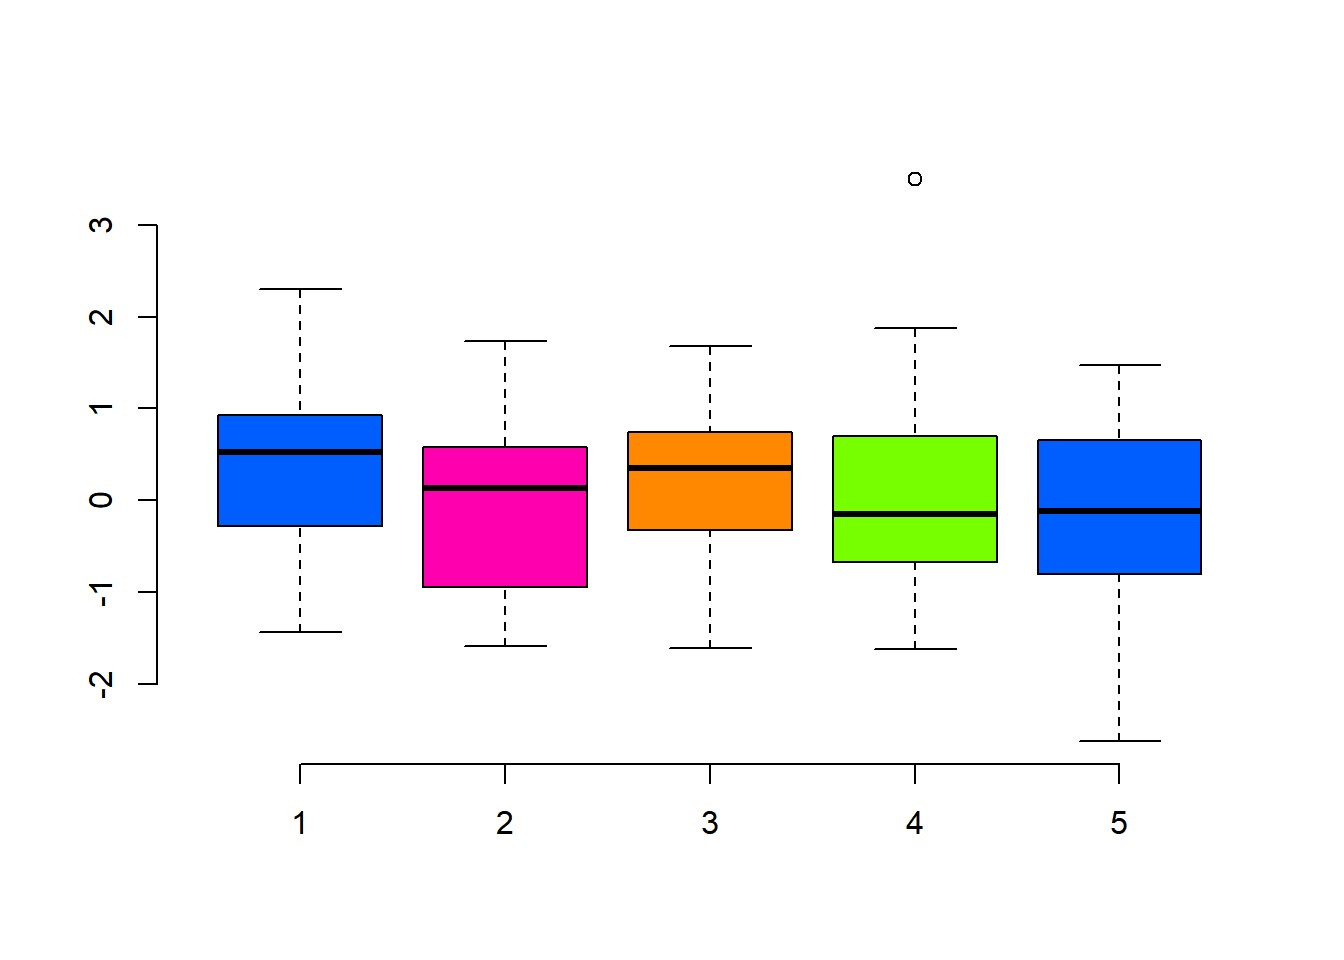
\includegraphics{myRBook_SP_files/figure-latex/unnamed-chunk-244-1.pdf}

Con la función \texttt{rgb()} podemos representar 256\^{}3 colores, o
167 777 216 colores diferentes. Nuestro objetivo, sin embargo, es hacer
gráficos que sean divertidos de leer y que hagan un buen uso de nuestros
resultados científicos. Por lo tanto, debemos elegir los colores
adecuados para nuestro propósito. Por eso utilizaremos paletas de
colores.

\section{Paletas de colores}\label{paletas-de-colores}

Las paletas son esquemas de color representados como un \texttt{vector}
con colores en formato hexadecimal (valor devuelto por la función
\texttt{rgb()}).

\begin{Shaded}
\begin{Highlighting}[]
\NormalTok{myPal <-}\StringTok{ }\KeywordTok{c}\NormalTok{(}
  \KeywordTok{rgb}\NormalTok{(}\DecValTok{0}\NormalTok{, }\DecValTok{94}\NormalTok{, }\DecValTok{255}\NormalTok{, }\DataTypeTok{maxColorValue =} \DecValTok{255}\NormalTok{),  }
  \KeywordTok{rgb}\NormalTok{(}\DecValTok{255}\NormalTok{, }\DecValTok{0}\NormalTok{, }\DecValTok{174}\NormalTok{, }\DataTypeTok{maxColorValue =} \DecValTok{255}\NormalTok{),  }
  \KeywordTok{rgb}\NormalTok{(}\DecValTok{255}\NormalTok{, }\DecValTok{136}\NormalTok{, }\DecValTok{0}\NormalTok{, }\DataTypeTok{maxColorValue =} \DecValTok{255}\NormalTok{),  }
  \KeywordTok{rgb}\NormalTok{(}\DecValTok{119}\NormalTok{, }\DecValTok{255}\NormalTok{, }\DecValTok{0}\NormalTok{, }\DataTypeTok{maxColorValue =} \DecValTok{255}\NormalTok{))}
\KeywordTok{print}\NormalTok{(myPal)}
\end{Highlighting}
\end{Shaded}

\begin{verbatim}
## [1] "#005EFF" "#FF00AE" "#FF8800" "#77FF00"
\end{verbatim}

\begin{Shaded}
\begin{Highlighting}[]
\KeywordTok{boxplot}\NormalTok{(}\KeywordTok{matrix}\NormalTok{(}\KeywordTok{rnorm}\NormalTok{(}\DecValTok{100}\NormalTok{), }\DataTypeTok{ncol =} \DecValTok{5}\NormalTok{), }\DataTypeTok{col =}\NormalTok{ myPal, }\DataTypeTok{axes =} \OtherTok{FALSE}\NormalTok{)}
\KeywordTok{axis}\NormalTok{(}\DecValTok{1}\NormalTok{)}
\KeywordTok{axis}\NormalTok{(}\DecValTok{2}\NormalTok{)}
\end{Highlighting}
\end{Shaded}

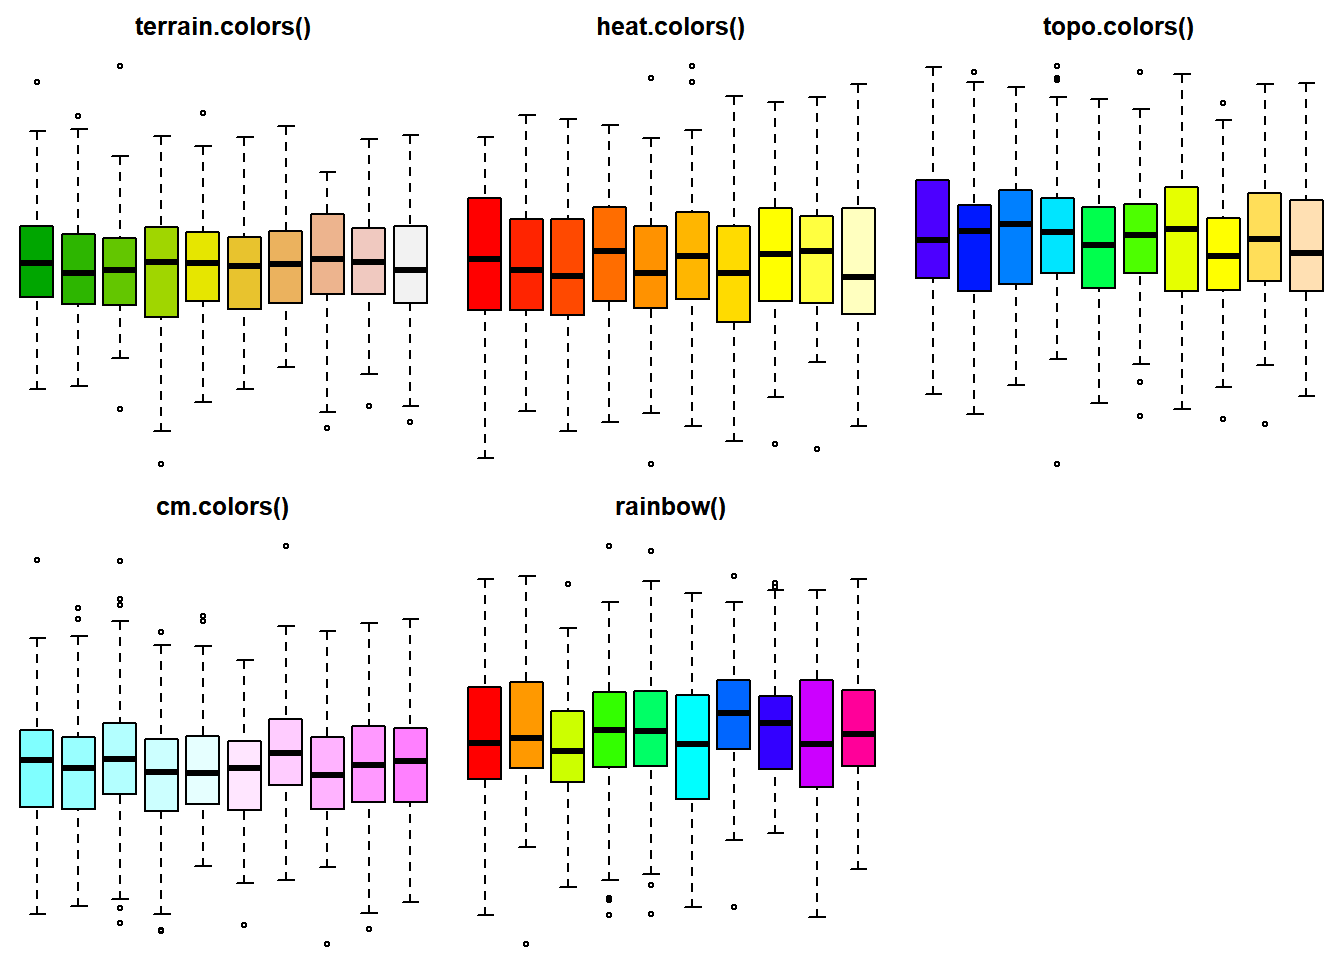
\includegraphics{myRBook_SP_files/figure-latex/unnamed-chunk-245-1.pdf}

Hay paletas de colores incluidos en R: \texttt{terrain.colors()},
\texttt{heat.colors()}, \texttt{topo.colors()}, \texttt{cm.colors()},
\texttt{rainbow()}.

\begin{Shaded}
\begin{Highlighting}[]
\NormalTok{op <-}\StringTok{ }\KeywordTok{par}\NormalTok{(}\DataTypeTok{no.readonly =} \OtherTok{TRUE}\NormalTok{)}
\KeywordTok{par}\NormalTok{(}\DataTypeTok{mfrow =} \KeywordTok{c}\NormalTok{(}\DecValTok{2}\NormalTok{, }\DecValTok{3}\NormalTok{), }\DataTypeTok{mar =} \KeywordTok{c}\NormalTok{(}\DecValTok{0}\NormalTok{, }\DecValTok{0}\NormalTok{, }\DecValTok{2}\NormalTok{, }\DecValTok{0}\NormalTok{))}
\KeywordTok{boxplot}\NormalTok{(}\KeywordTok{matrix}\NormalTok{(}\KeywordTok{rnorm}\NormalTok{(}\DecValTok{1000}\NormalTok{), }\DataTypeTok{ncol =} \DecValTok{10}\NormalTok{), }\DataTypeTok{main =} \StringTok{"terrain.colors()"}\NormalTok{, }
        \DataTypeTok{col =} \KeywordTok{terrain.colors}\NormalTok{(}\DecValTok{10}\NormalTok{), }\DataTypeTok{axes =} \OtherTok{FALSE}\NormalTok{)}
\KeywordTok{boxplot}\NormalTok{(}\KeywordTok{matrix}\NormalTok{(}\KeywordTok{rnorm}\NormalTok{(}\DecValTok{1000}\NormalTok{), }\DataTypeTok{ncol =} \DecValTok{10}\NormalTok{), }\DataTypeTok{main =} \StringTok{"heat.colors()"}\NormalTok{, }
        \DataTypeTok{col =} \KeywordTok{heat.colors}\NormalTok{(}\DecValTok{10}\NormalTok{), }\DataTypeTok{axes =} \OtherTok{FALSE}\NormalTok{)}
\KeywordTok{boxplot}\NormalTok{(}\KeywordTok{matrix}\NormalTok{(}\KeywordTok{rnorm}\NormalTok{(}\DecValTok{1000}\NormalTok{), }\DataTypeTok{ncol =} \DecValTok{10}\NormalTok{), }\DataTypeTok{main =} \StringTok{"topo.colors()"}\NormalTok{, }
        \DataTypeTok{col =} \KeywordTok{topo.colors}\NormalTok{(}\DecValTok{10}\NormalTok{), }\DataTypeTok{axes =} \OtherTok{FALSE}\NormalTok{)}
\KeywordTok{boxplot}\NormalTok{(}\KeywordTok{matrix}\NormalTok{(}\KeywordTok{rnorm}\NormalTok{(}\DecValTok{1000}\NormalTok{), }\DataTypeTok{ncol =} \DecValTok{10}\NormalTok{), }\DataTypeTok{main =} \StringTok{"cm.colors()"}\NormalTok{, }
        \DataTypeTok{col =} \KeywordTok{cm.colors}\NormalTok{(}\DecValTok{10}\NormalTok{), }\DataTypeTok{axes =} \OtherTok{FALSE}\NormalTok{)}
\KeywordTok{boxplot}\NormalTok{(}\KeywordTok{matrix}\NormalTok{(}\KeywordTok{rnorm}\NormalTok{(}\DecValTok{1000}\NormalTok{), }\DataTypeTok{ncol =} \DecValTok{10}\NormalTok{), }\DataTypeTok{main =} \StringTok{"rainbow()"}\NormalTok{, }
        \DataTypeTok{col =} \KeywordTok{rainbow}\NormalTok{(}\DecValTok{10}\NormalTok{), }\DataTypeTok{axes =} \OtherTok{FALSE}\NormalTok{)}
\KeywordTok{par}\NormalTok{(op)}
\end{Highlighting}
\end{Shaded}

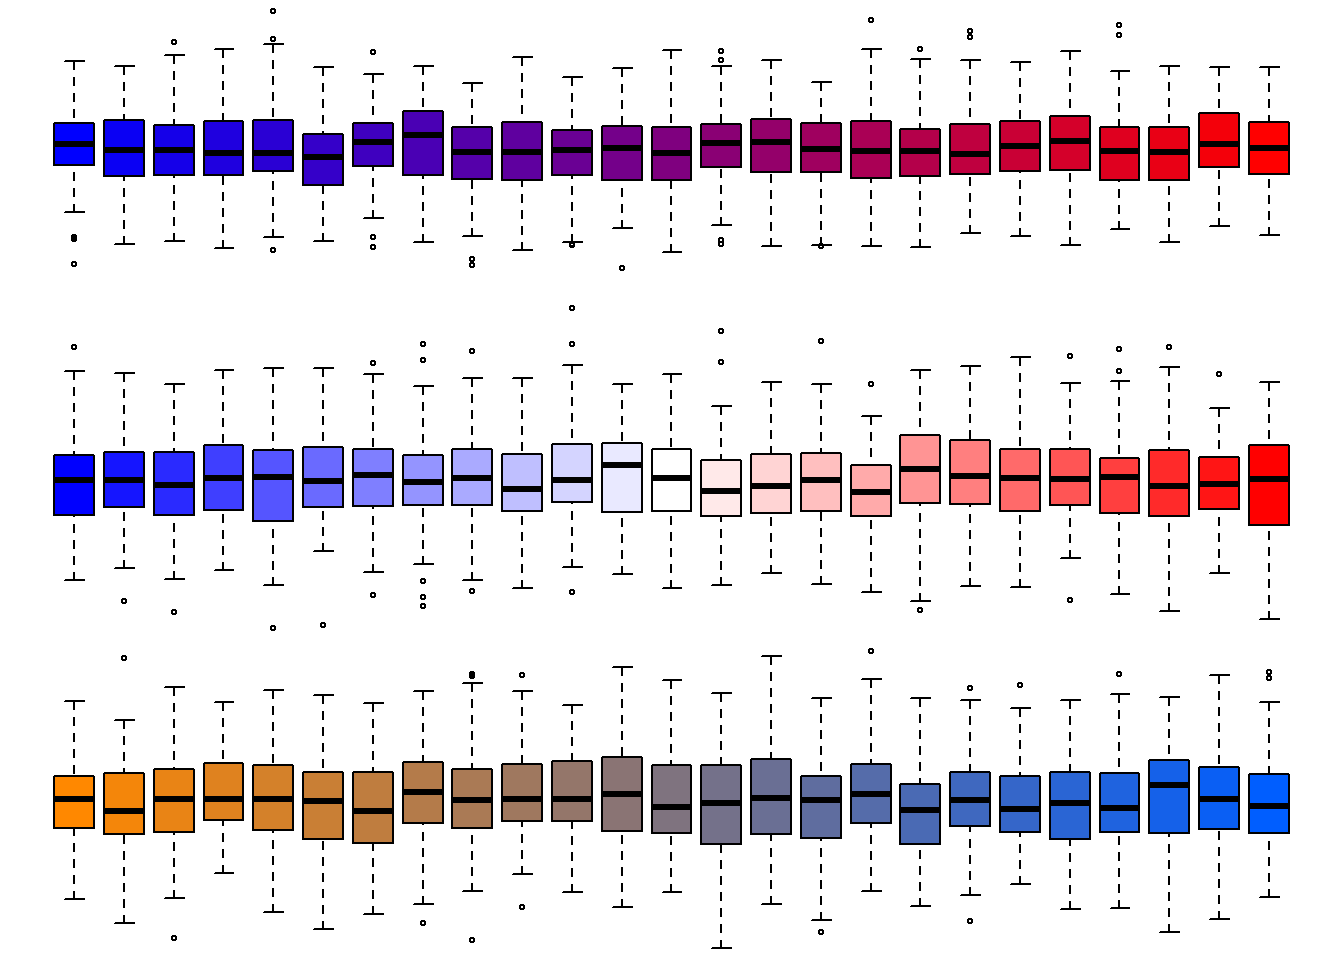
\includegraphics{myRBook_SP_files/figure-latex/unnamed-chunk-246-1.pdf}

También hay una función \texttt{colorRampPalette()} que nos permite
crear un degradado de color.

\begin{Shaded}
\begin{Highlighting}[]
\NormalTok{op <-}\StringTok{ }\KeywordTok{par}\NormalTok{(}\DataTypeTok{no.readonly =} \OtherTok{TRUE}\NormalTok{)}
\KeywordTok{par}\NormalTok{(}\DataTypeTok{mfrow =} \KeywordTok{c}\NormalTok{(}\DecValTok{3}\NormalTok{, }\DecValTok{1}\NormalTok{), }\DataTypeTok{mar =} \KeywordTok{c}\NormalTok{(}\DecValTok{0}\NormalTok{, }\DecValTok{0}\NormalTok{, }\DecValTok{0}\NormalTok{, }\DecValTok{0}\NormalTok{))}
\KeywordTok{boxplot}\NormalTok{(}\KeywordTok{matrix}\NormalTok{(}\KeywordTok{rnorm}\NormalTok{(}\DecValTok{2500}\NormalTok{), }\DataTypeTok{ncol =} \DecValTok{25}\NormalTok{), }
        \DataTypeTok{col =} \KeywordTok{colorRampPalette}\NormalTok{(}\KeywordTok{c}\NormalTok{(}\StringTok{'blue'}\NormalTok{, }\StringTok{'red'}\NormalTok{))(}\DecValTok{25}\NormalTok{), }\DataTypeTok{axes =} \OtherTok{FALSE}\NormalTok{)}
\KeywordTok{boxplot}\NormalTok{(}\KeywordTok{matrix}\NormalTok{(}\KeywordTok{rnorm}\NormalTok{(}\DecValTok{2500}\NormalTok{), }\DataTypeTok{ncol =} \DecValTok{25}\NormalTok{), }
        \DataTypeTok{col =} \KeywordTok{colorRampPalette}\NormalTok{(}\KeywordTok{c}\NormalTok{(}\StringTok{'blue'}\NormalTok{, }\StringTok{'white'}\NormalTok{, }\StringTok{'red'}\NormalTok{))(}\DecValTok{25}\NormalTok{), }\DataTypeTok{axes =} \OtherTok{FALSE}\NormalTok{)}
\KeywordTok{boxplot}\NormalTok{(}\KeywordTok{matrix}\NormalTok{(}\KeywordTok{rnorm}\NormalTok{(}\DecValTok{2500}\NormalTok{), }\DataTypeTok{ncol =} \DecValTok{25}\NormalTok{), }
        \DataTypeTok{col =}  \KeywordTok{colorRampPalette}\NormalTok{(}\KeywordTok{c}\NormalTok{(}\KeywordTok{rgb}\NormalTok{(}\DecValTok{255}\NormalTok{, }\DecValTok{136}\NormalTok{, }\DecValTok{0}\NormalTok{, }\DataTypeTok{maxColorValue =} \DecValTok{255}\NormalTok{),  }
                                  \KeywordTok{rgb}\NormalTok{(}\DecValTok{0}\NormalTok{, }\DecValTok{94}\NormalTok{, }\DecValTok{255}\NormalTok{, }\DataTypeTok{maxColorValue =} \DecValTok{255}\NormalTok{)))(}\DecValTok{25}\NormalTok{), }
        \DataTypeTok{axes =} \OtherTok{FALSE}\NormalTok{)}
\end{Highlighting}
\end{Shaded}

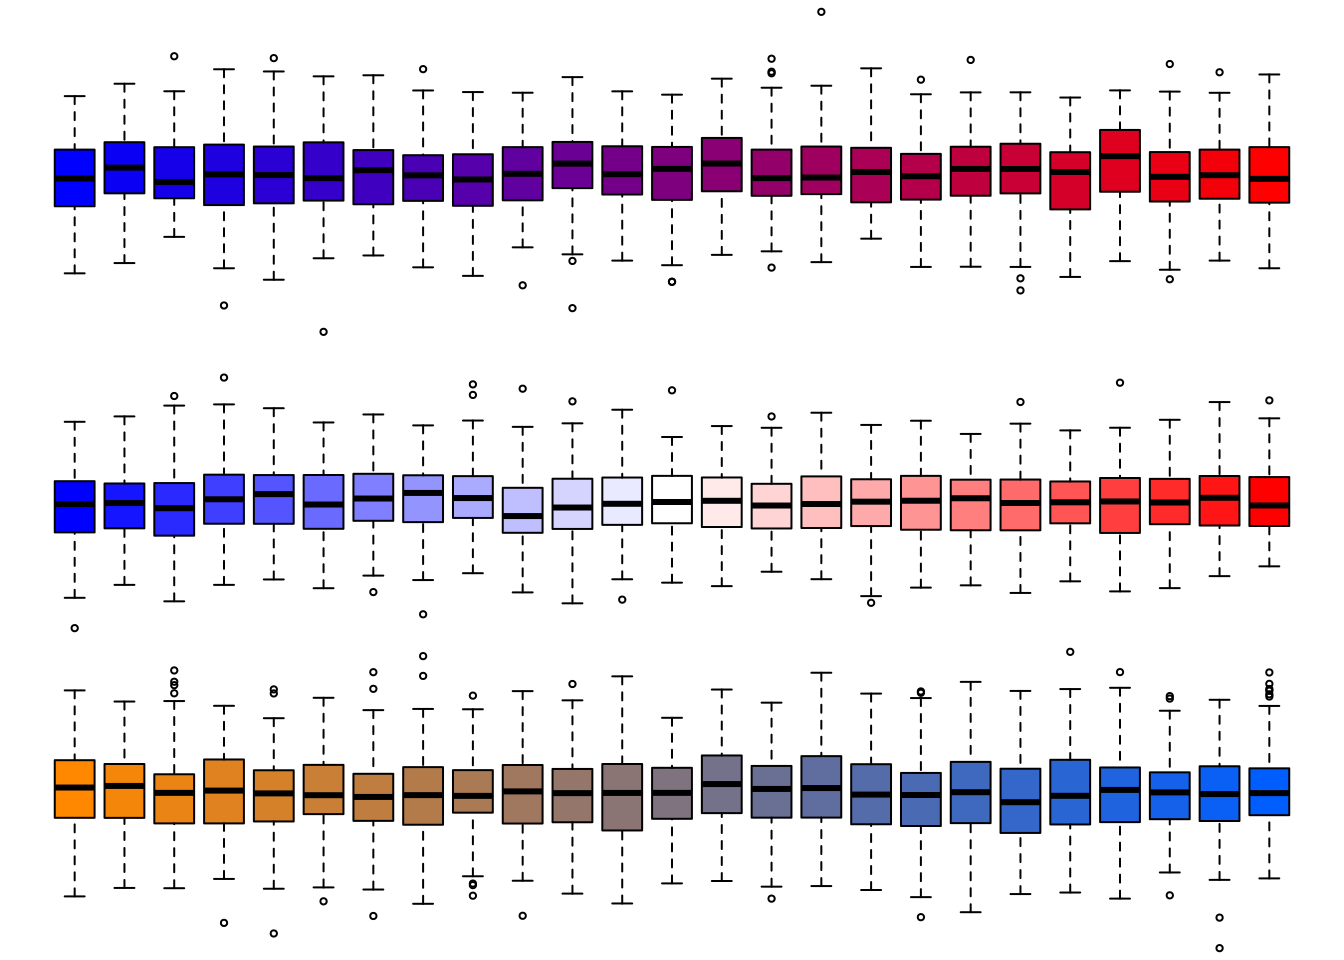
\includegraphics{myRBook_SP_files/figure-latex/unnamed-chunk-247-1.pdf}

\begin{Shaded}
\begin{Highlighting}[]
\KeywordTok{par}\NormalTok{(op)}
\end{Highlighting}
\end{Shaded}

También podemos crear nuestras propias paletas utilizando sitios web de
selección de colores como \url{http://paletton.com/} o
\url{https://coolors.co/} (hay muchos más), y luego utilizarlos en R
copiando en un \texttt{vector} los valores hexadecimales o rgb.

R es un lenguaje de programación muy poderoso. Podemos imaginar muchas
formas de crear paletas automáticamente de acuerdo con varios criterios.
Por ejemplo, podemos importar una imagen cuyos tonos nos parezcan
relevantes, luego extraer la información de cada uno de los puntos y
luego seleccionar los colores dominantes a través de una agrupación tipo
\texttt{kmeans}. Eso es lo que hace la siguiente función.

Primero, cargaremos los paquetes \texttt{raster},\texttt{rgdal} y
\texttt{jpeg} que se utilizarán para manipular nuestra imagen en R.

\begin{Shaded}
\begin{Highlighting}[]
\NormalTok{pkgCheck <-}\StringTok{ }\ControlFlowTok{function}\NormalTok{(x)\{ }
  \ControlFlowTok{if}\NormalTok{ (}\OperatorTok{!}\KeywordTok{require}\NormalTok{(x, }\DataTypeTok{character.only =} \OtherTok{TRUE}\NormalTok{))\{}
    \KeywordTok{install.packages}\NormalTok{(x, }\DataTypeTok{dependencies =} \OtherTok{TRUE}\NormalTok{)}
      \ControlFlowTok{if}\NormalTok{(}\OperatorTok{!}\KeywordTok{require}\NormalTok{(x, }\DataTypeTok{character.only =} \OtherTok{TRUE}\NormalTok{)) \{}
        \KeywordTok{stop}\NormalTok{()}
\NormalTok{    \}}
\NormalTok{  \}}
\NormalTok{\}}
\KeywordTok{pkgCheck}\NormalTok{(}\StringTok{"raster"}\NormalTok{)}
\KeywordTok{pkgCheck}\NormalTok{(}\StringTok{"rgdal"}\NormalTok{)}
\KeywordTok{pkgCheck}\NormalTok{(}\StringTok{"jpeg"}\NormalTok{)}
\end{Highlighting}
\end{Shaded}

Luego usaremos la función \texttt{kmeans()} para realizar grupos de
colores usando los valores RGB de cada punto en nuestra imagen. Aquí
tenemos dos métodos posibles, el primero usa la función
\texttt{kmeans()} para los tres valores RGB, y el segundo usa la función
\texttt{kmeans()} para cada valor RGB individualmente (esta segunda
función proporciona una paleta que puede ser bastante alejado de los
colores de la imagen original).

\begin{Shaded}
\begin{Highlighting}[]
\NormalTok{createPal <-}\StringTok{ }\ControlFlowTok{function}\NormalTok{(photo, }\DataTypeTok{met =} \DecValTok{1}\NormalTok{, }\DataTypeTok{graph =} \OtherTok{TRUE}\NormalTok{, }\DataTypeTok{k =} \DecValTok{9}\NormalTok{)\{}
  \ControlFlowTok{if}\NormalTok{(met }\OperatorTok{==}\StringTok{ }\DecValTok{1}\NormalTok{)\{}
\NormalTok{    colR <-}\StringTok{ }\KeywordTok{getValues}\NormalTok{(}\KeywordTok{raster}\NormalTok{(photo, }\DataTypeTok{band =} \DecValTok{1}\NormalTok{))}
\NormalTok{    colG <-}\StringTok{ }\KeywordTok{getValues}\NormalTok{(}\KeywordTok{raster}\NormalTok{(photo, }\DataTypeTok{band =} \DecValTok{2}\NormalTok{))}
\NormalTok{    colB <-}\StringTok{ }\KeywordTok{getValues}\NormalTok{(}\KeywordTok{raster}\NormalTok{(photo, }\DataTypeTok{band =} \DecValTok{3}\NormalTok{))}
\NormalTok{    kMeans <-}\StringTok{ }\KeywordTok{kmeans}\NormalTok{(}\KeywordTok{data.frame}\NormalTok{(colR, colG, colB), }\DataTypeTok{centers =}\NormalTok{ k)}
\NormalTok{    kCol <-}\StringTok{ }\KeywordTok{rgb}\NormalTok{(kMeans}\OperatorTok{$}\NormalTok{centers, }\DataTypeTok{maxColorValue =} \DecValTok{255}\NormalTok{)[}\KeywordTok{order}\NormalTok{(}\KeywordTok{table}\NormalTok{(}
\NormalTok{      kMeans}\OperatorTok{$}\NormalTok{cluster), }\DataTypeTok{decreasing =} \OtherTok{TRUE}\NormalTok{)]}
    \ControlFlowTok{if}\NormalTok{(graph }\OperatorTok{==}\StringTok{ }\OtherTok{TRUE}\NormalTok{)\{}
\NormalTok{      op <-}\StringTok{ }\KeywordTok{par}\NormalTok{(}\DataTypeTok{no.readonly =} \OtherTok{TRUE}\NormalTok{)}
      \KeywordTok{par}\NormalTok{(}\DataTypeTok{mfrow =} \KeywordTok{c}\NormalTok{ (}\DecValTok{1}\NormalTok{, }\DecValTok{2}\NormalTok{), }\DataTypeTok{mar =} \KeywordTok{c}\NormalTok{(}\DecValTok{0}\NormalTok{, }\DecValTok{2}\NormalTok{, }\DecValTok{2}\NormalTok{, }\DecValTok{0}\NormalTok{))}
\NormalTok{      myJpg <-}\StringTok{ }\KeywordTok{readJPEG}\NormalTok{(}\StringTok{"./myFiles/photoKmeans.jpg"}\NormalTok{, }\DataTypeTok{native =} \OtherTok{TRUE}\NormalTok{)}
      \KeywordTok{plot}\NormalTok{(}\DecValTok{0}\OperatorTok{:}\DecValTok{1}\NormalTok{, }\DecValTok{0}\OperatorTok{:}\DecValTok{1}\NormalTok{, }\DataTypeTok{type =} \StringTok{"n"}\NormalTok{, }\DataTypeTok{ann =} \OtherTok{FALSE}\NormalTok{, }\DataTypeTok{axes =} \OtherTok{FALSE}\NormalTok{)}
      \KeywordTok{rasterImage}\NormalTok{(myJpg, }\DecValTok{0}\NormalTok{, }\DecValTok{0}\NormalTok{, }\DecValTok{1}\NormalTok{, }\DecValTok{1}\NormalTok{)}
      \KeywordTok{barplot}\NormalTok{(}\KeywordTok{table}\NormalTok{(kMeans}\OperatorTok{$}\NormalTok{cluster)[}\KeywordTok{order}\NormalTok{(}\KeywordTok{table}\NormalTok{(kMeans}\OperatorTok{$}\NormalTok{cluster), }
        \DataTypeTok{decreasing =} \OtherTok{TRUE}\NormalTok{)], }\DataTypeTok{col =}\NormalTok{ kCol, }\DataTypeTok{names.arg =} \OtherTok{NA}\NormalTok{)}
      \KeywordTok{par}\NormalTok{(op)}
\NormalTok{    \}}
    \KeywordTok{return}\NormalTok{(kCol)}
\NormalTok{  \} }\ControlFlowTok{else}\NormalTok{ \{}
    \ControlFlowTok{if}\NormalTok{(met }\OperatorTok{==}\StringTok{ }\DecValTok{2}\NormalTok{)\{}
\NormalTok{      kColR <-}\StringTok{ }\KeywordTok{kmeans}\NormalTok{(}\DataTypeTok{x =} \KeywordTok{getValues}\NormalTok{(}\KeywordTok{raster}\NormalTok{(photo, }\DataTypeTok{band =} \DecValTok{1}\NormalTok{)), }
                      \DataTypeTok{centers =}\NormalTok{ k)}
\NormalTok{      kColG <-}\StringTok{ }\KeywordTok{kmeans}\NormalTok{(}\DataTypeTok{x =} \KeywordTok{getValues}\NormalTok{(}\KeywordTok{raster}\NormalTok{(photo, }\DataTypeTok{band =} \DecValTok{2}\NormalTok{)), }
                      \DataTypeTok{centers =}\NormalTok{ k)}
\NormalTok{      kColB <-}\StringTok{ }\KeywordTok{kmeans}\NormalTok{(}\DataTypeTok{x =} \KeywordTok{getValues}\NormalTok{(}\KeywordTok{raster}\NormalTok{(photo, }\DataTypeTok{band =} \DecValTok{3}\NormalTok{)), }
                      \DataTypeTok{centers =}\NormalTok{ k)}
\NormalTok{      kCol <-}\StringTok{ }\NormalTok{(}\KeywordTok{rgb}\NormalTok{(kColR}\OperatorTok{$}\NormalTok{centers, kColG}\OperatorTok{$}\NormalTok{centers, kColB}\OperatorTok{$}\NormalTok{centers,}
                   \DataTypeTok{maxColorValue =} \DecValTok{255}\NormalTok{))}
      \ControlFlowTok{if}\NormalTok{(graph }\OperatorTok{==}\StringTok{ }\OtherTok{TRUE}\NormalTok{)\{}
\NormalTok{        op <-}\StringTok{ }\KeywordTok{par}\NormalTok{(}\DataTypeTok{no.readonly =} \OtherTok{TRUE}\NormalTok{)}
        \KeywordTok{par}\NormalTok{(}\DataTypeTok{mfrow =} \KeywordTok{c}\NormalTok{ (}\DecValTok{1}\NormalTok{, }\DecValTok{2}\NormalTok{), }\DataTypeTok{mar =} \KeywordTok{c}\NormalTok{(}\DecValTok{0}\NormalTok{, }\DecValTok{2}\NormalTok{, }\DecValTok{2}\NormalTok{, }\DecValTok{0}\NormalTok{))}
\NormalTok{        myJpg <-}\StringTok{ }\KeywordTok{readJPEG}\NormalTok{(}\StringTok{"./myFiles/photoKmeans.jpg"}\NormalTok{, }\DataTypeTok{native =} \OtherTok{TRUE}\NormalTok{)}
        \KeywordTok{plot}\NormalTok{(}\DecValTok{0}\OperatorTok{:}\DecValTok{1}\NormalTok{, }\DecValTok{0}\OperatorTok{:}\DecValTok{1}\NormalTok{, }\DataTypeTok{type =} \StringTok{"n"}\NormalTok{, }\DataTypeTok{ann =} \OtherTok{FALSE}\NormalTok{, }\DataTypeTok{axes =} \OtherTok{FALSE}\NormalTok{)}
        \KeywordTok{rasterImage}\NormalTok{(myJpg, }\DecValTok{0}\NormalTok{, }\DecValTok{0}\NormalTok{, }\DecValTok{1}\NormalTok{, }\DecValTok{1}\NormalTok{)}
        \KeywordTok{plot}\NormalTok{(}\DataTypeTok{x =} \DecValTok{1}\OperatorTok{:}\NormalTok{k, }\DataTypeTok{y =} \KeywordTok{rep}\NormalTok{(}\DecValTok{1}\NormalTok{, k), }\DataTypeTok{ylim =} \KeywordTok{c}\NormalTok{(}\DecValTok{0}\NormalTok{, }\DecValTok{1}\NormalTok{), }
             \DataTypeTok{xlim =} \KeywordTok{c}\NormalTok{(}\DecValTok{0}\NormalTok{, k), }\DataTypeTok{axes =} \OtherTok{FALSE}\NormalTok{, }\DataTypeTok{xlab =} \StringTok{""}\NormalTok{, }
             \DataTypeTok{ylab =} \StringTok{""}\NormalTok{, }\DataTypeTok{type =} \StringTok{"n"}\NormalTok{)}
        \ControlFlowTok{for}\NormalTok{(i }\ControlFlowTok{in} \DecValTok{1}\OperatorTok{:}\NormalTok{k)\{}
          \KeywordTok{polygon}\NormalTok{(}\DataTypeTok{x =} \KeywordTok{c}\NormalTok{(i}\OperatorTok{-}\DecValTok{1}\NormalTok{, i, i, i}\OperatorTok{-}\DecValTok{1}\NormalTok{), }\DataTypeTok{y =} \KeywordTok{c}\NormalTok{(}\DecValTok{0}\NormalTok{, }\DecValTok{0}\NormalTok{, }\DecValTok{1}\NormalTok{, }\DecValTok{1}\NormalTok{), }
                  \DataTypeTok{col =}\NormalTok{ kCol[i])}
          \KeywordTok{text}\NormalTok{(}\DataTypeTok{x =}\NormalTok{ i }\OperatorTok{-}\StringTok{ }\FloatTok{0.5}\NormalTok{, }\DataTypeTok{y =} \FloatTok{0.5}\NormalTok{, }
               \DataTypeTok{labels =} \KeywordTok{as.character}\NormalTok{(kCol[i]), }\DataTypeTok{srt =} \DecValTok{90}\NormalTok{)}
\NormalTok{        \}}
        \KeywordTok{par}\NormalTok{(op)}
\NormalTok{      \}}
      \KeywordTok{return}\NormalTok{(kCol)}
\NormalTok{    \} }\ControlFlowTok{else}\NormalTok{ \{}
      \KeywordTok{print}\NormalTok{(}\KeywordTok{paste0}\NormalTok{(}\StringTok{"No method "}\NormalTok{, met, }\StringTok{"."}\NormalTok{))}
      \KeywordTok{return}\NormalTok{(}\KeywordTok{rgb}\NormalTok{(}\DecValTok{0}\NormalTok{, }\DecValTok{0}\NormalTok{, }\DecValTok{0}\NormalTok{))}
\NormalTok{    \}}
\NormalTok{  \}}
\NormalTok{\}}

\NormalTok{myPalMet1 <-}\StringTok{ }\KeywordTok{createPal}\NormalTok{(}\DataTypeTok{photo =} \StringTok{"./myFiles/photoKmeans.jpg"}\NormalTok{, }
                       \DataTypeTok{met =} \DecValTok{1}\NormalTok{, }\DataTypeTok{graph =} \OtherTok{TRUE}\NormalTok{, }\DataTypeTok{k =} \DecValTok{5}\NormalTok{)}
\end{Highlighting}
\end{Shaded}

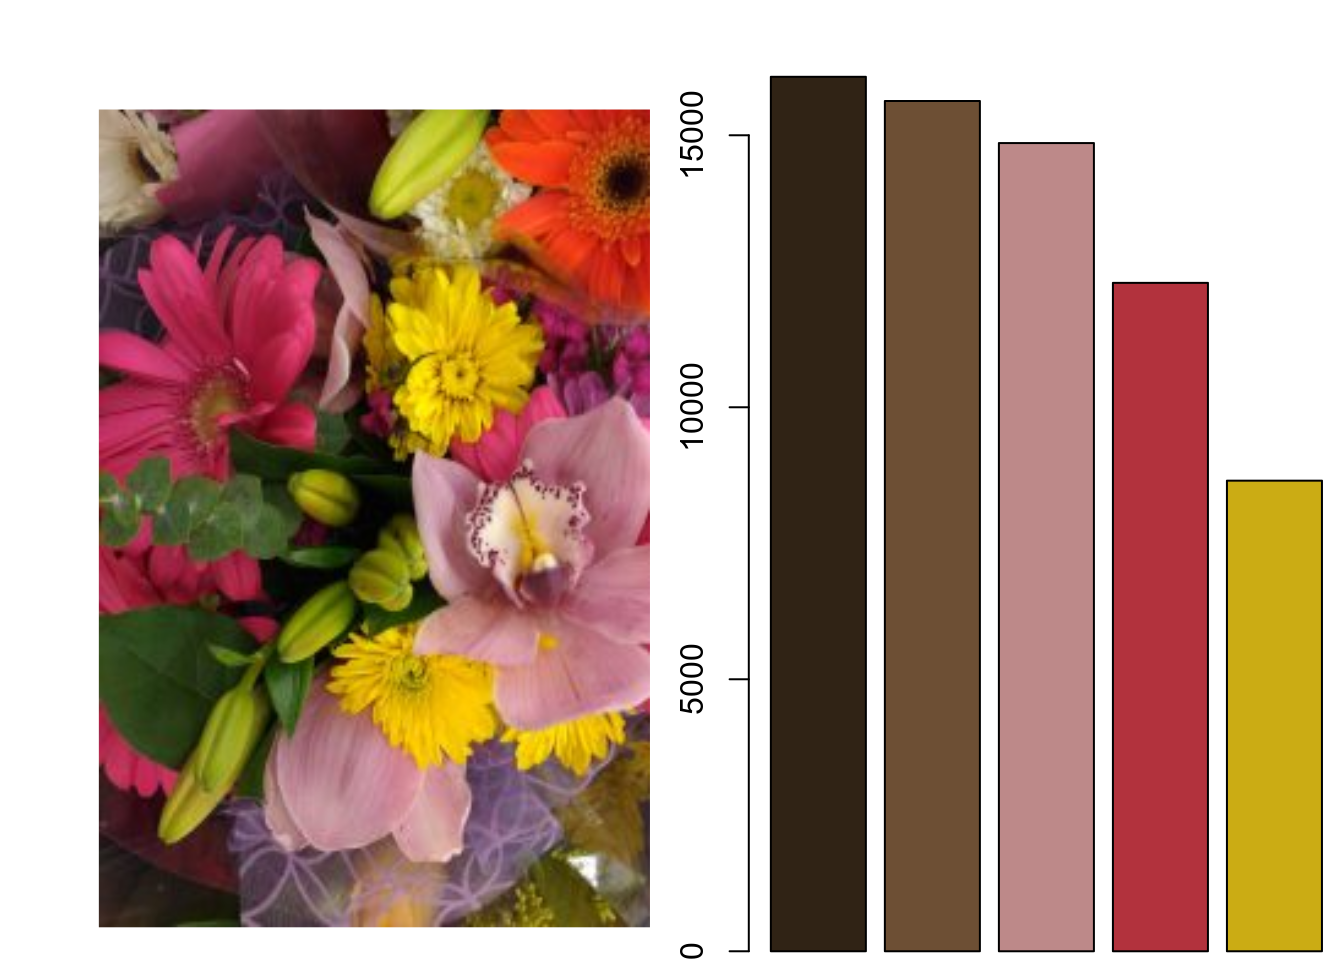
\includegraphics{myRBook_SP_files/figure-latex/unnamed-chunk-249-1.pdf}

\begin{Shaded}
\begin{Highlighting}[]
\NormalTok{myPalMet2 <-}\StringTok{ }\KeywordTok{createPal}\NormalTok{(}\DataTypeTok{photo =} \StringTok{"./myFiles/photoKmeans.jpg"}\NormalTok{, }
                       \DataTypeTok{met =} \DecValTok{2}\NormalTok{, }\DataTypeTok{graph =} \OtherTok{TRUE}\NormalTok{, }\DataTypeTok{k =} \DecValTok{5}\NormalTok{)}
\end{Highlighting}
\end{Shaded}

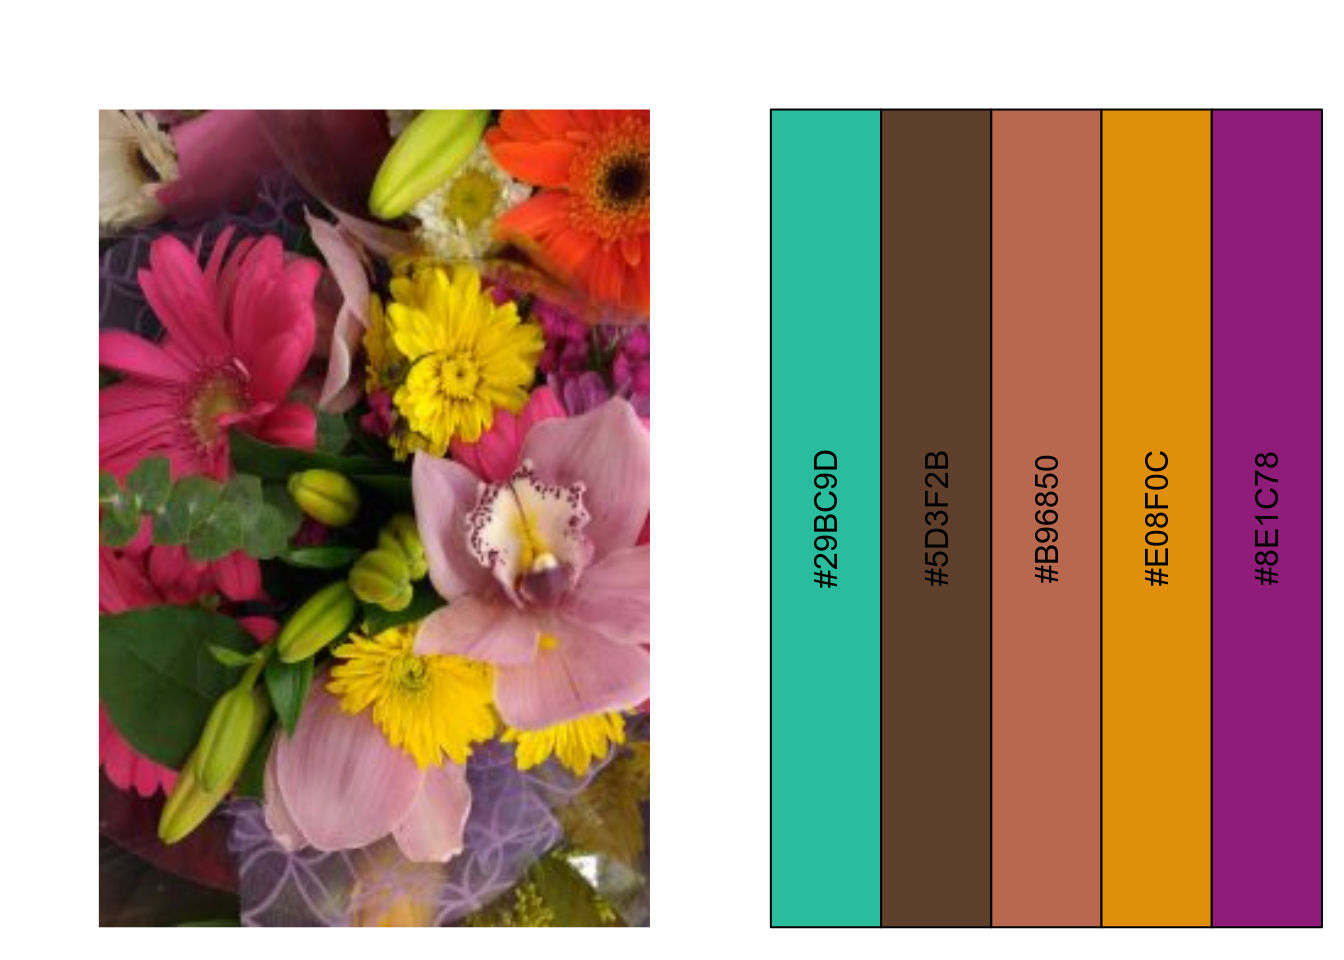
\includegraphics{myRBook_SP_files/figure-latex/unnamed-chunk-249-2.pdf}

La función nos devuelve los colores de la paleta con un gráfico de
barras que representa el número de puntos de la imagen en cada uno de
los grupos de colores. Ahora podemos usar nuestra nueva paleta para
hacer nuestros gráficos.

\begin{Shaded}
\begin{Highlighting}[]
\NormalTok{makeImpact <-}\StringTok{ }\ControlFlowTok{function}\NormalTok{(myPal, }\DataTypeTok{numP =} \DecValTok{300}\NormalTok{, }\DataTypeTok{impact =} \FloatTok{0.33}\NormalTok{, }\DataTypeTok{multCex =} \DecValTok{3}\NormalTok{)\{}
\NormalTok{  myX <-}\StringTok{ }\KeywordTok{sample}\NormalTok{(}\DecValTok{0}\OperatorTok{:}\DecValTok{1000}\NormalTok{, }\DataTypeTok{size =}\NormalTok{ numP, }\DataTypeTok{replace =} \OtherTok{TRUE}\NormalTok{)}\OperatorTok{/}\DecValTok{1000}
\NormalTok{  myY <-}\StringTok{ }\KeywordTok{sample}\NormalTok{(}\DecValTok{0}\OperatorTok{:}\DecValTok{1000}\NormalTok{, }\DataTypeTok{size =}\NormalTok{ numP, }\DataTypeTok{replace =} \OtherTok{TRUE}\NormalTok{)}\OperatorTok{/}\DecValTok{1000}
\NormalTok{  distImpact <-}\StringTok{ }\KeywordTok{sqrt}\NormalTok{((myX }\OperatorTok{-}\StringTok{ }\NormalTok{impact)}\OperatorTok{^}\DecValTok{2} \OperatorTok{+}\StringTok{ }\NormalTok{(myY }\OperatorTok{-}\StringTok{ }\NormalTok{impact)}\OperatorTok{^}\DecValTok{2}\NormalTok{)}
\NormalTok{  dfXY <-}\StringTok{ }\KeywordTok{data.frame}\NormalTok{(myX, myY, distImpact)}
  \KeywordTok{plot}\NormalTok{(}\DataTypeTok{x =}\NormalTok{ dfXY}\OperatorTok{$}\NormalTok{myX, }\DataTypeTok{y =}\NormalTok{ dfXY}\OperatorTok{$}\NormalTok{myY, }\DataTypeTok{axes =} \OtherTok{FALSE}\NormalTok{, }
    \DataTypeTok{xlab =} \StringTok{""}\NormalTok{, }\DataTypeTok{ylab =} \StringTok{""}\NormalTok{, }\DataTypeTok{cex =}\NormalTok{ dfXY}\OperatorTok{$}\NormalTok{distImpact}\OperatorTok{*}\NormalTok{multCex, }
    \DataTypeTok{col =}\NormalTok{ myPal, }\DataTypeTok{pch =} \DecValTok{16}\NormalTok{)}
\NormalTok{\}}

\NormalTok{op <-}\StringTok{ }\KeywordTok{par}\NormalTok{(}\DataTypeTok{no.readonly =} \OtherTok{TRUE}\NormalTok{)}
\KeywordTok{par}\NormalTok{(}\DataTypeTok{mfrow =} \KeywordTok{c}\NormalTok{ (}\DecValTok{1}\NormalTok{, }\DecValTok{2}\NormalTok{), }\DataTypeTok{mar =} \KeywordTok{c}\NormalTok{(}\DecValTok{0}\NormalTok{, }\DecValTok{0}\NormalTok{, }\DecValTok{0}\NormalTok{, }\DecValTok{0}\NormalTok{))}
\KeywordTok{makeImpact}\NormalTok{(}\DataTypeTok{myPal =}\NormalTok{ myPalMet1, }\DataTypeTok{numP =} \DecValTok{3000}\NormalTok{, }\DataTypeTok{impact =} \FloatTok{0.33}\NormalTok{)}
\KeywordTok{makeImpact}\NormalTok{(}\DataTypeTok{myPal =}\NormalTok{ myPalMet2, }\DataTypeTok{numP =} \DecValTok{3000}\NormalTok{, }\DataTypeTok{impact =} \FloatTok{0.66}\NormalTok{)}
\end{Highlighting}
\end{Shaded}

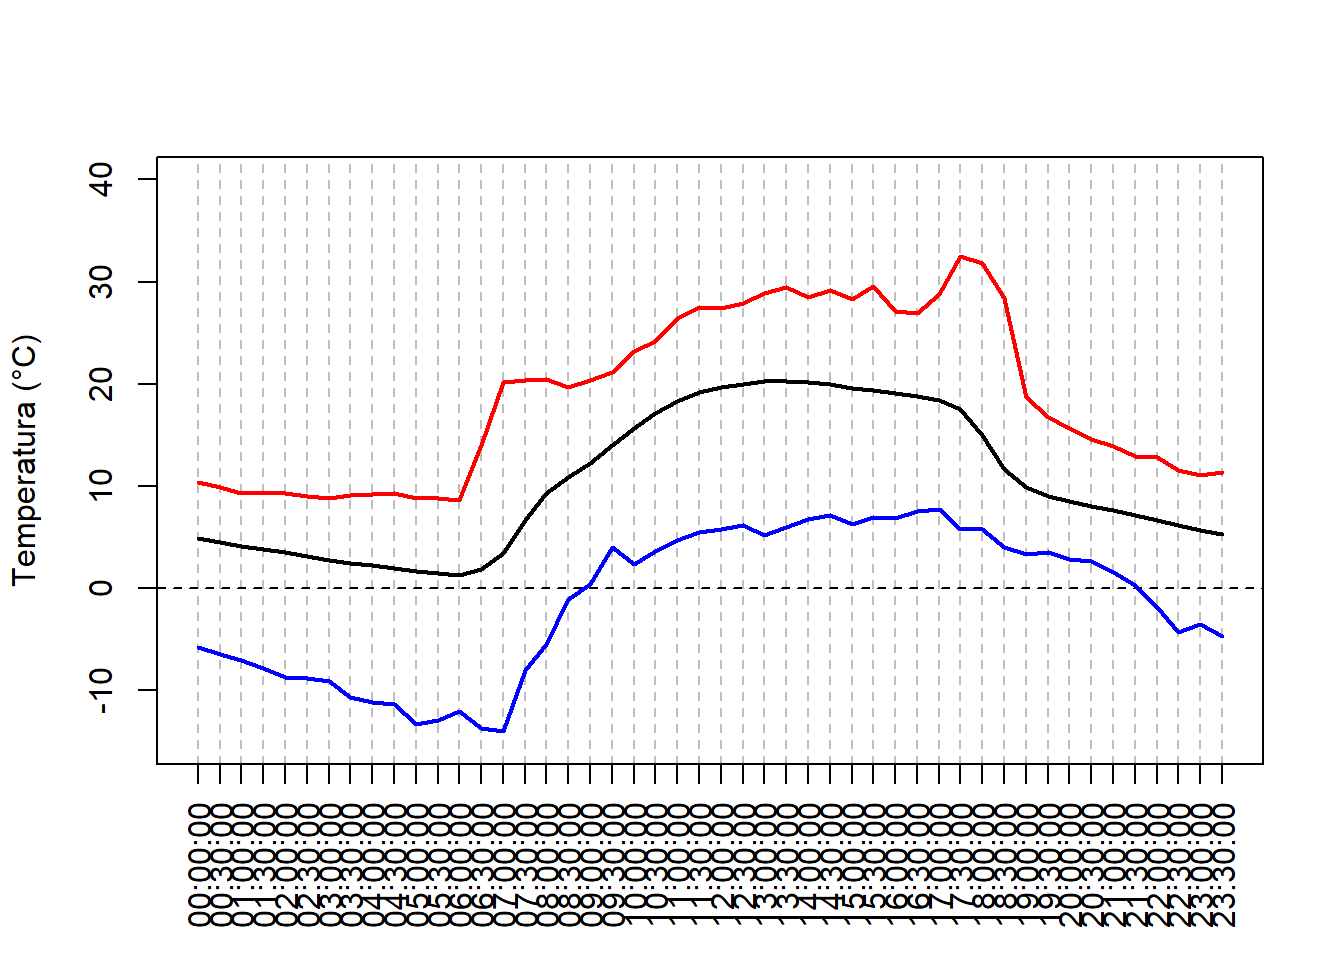
\includegraphics{myRBook_SP_files/figure-latex/unnamed-chunk-250-1.pdf}

\begin{Shaded}
\begin{Highlighting}[]
\KeywordTok{par}\NormalTok{(op)}
\end{Highlighting}
\end{Shaded}

\section{Conclusión}\label{conclusion-9}

Felicitaciones ! Este es el final de este capítulo sobre la gestión del
color. Ahora sabemos cómo usar colores y paletas, y cómo guiar la
selección de colores para resaltar nuestros resultados. En el siguiente
capítulo veremos algunos ejemplos de paquetes de gráficos y las últimas
tendencias, como los gráficos dinámicos.

\hypertarget{graph3}{\chapter{Paquetes gráficos}\label{graph3}}

\section{Los paquetes con paletas}\label{los-paquetes-con-paletas}

\subsection{\texorpdfstring{\texttt{RColorBrewer}}{RColorBrewer}}\label{rcolorbrewer}

El paquete \texttt{RColorBrewer} es un paquete de referencia porque
contiene paletas adicionales a las disponibles en la versión básica de
R. Una vez que el paquete está instalado, solo llamamos a las paletas
para utilizarlas. Aquí están las paletas disponibles y un ejemplo de
uso.

\begin{Shaded}
\begin{Highlighting}[]
\NormalTok{pkgCheck <-}\StringTok{ }\ControlFlowTok{function}\NormalTok{(x)\{ }
    \ControlFlowTok{if}\NormalTok{ (}\OperatorTok{!}\KeywordTok{require}\NormalTok{(x, }\DataTypeTok{character.only =} \OtherTok{TRUE}\NormalTok{))\{}
        \KeywordTok{install.packages}\NormalTok{(x, }\DataTypeTok{dependencies =} \OtherTok{TRUE}\NormalTok{)}
        \ControlFlowTok{if}\NormalTok{(}\OperatorTok{!}\KeywordTok{require}\NormalTok{(x, }\DataTypeTok{character.only =} \OtherTok{TRUE}\NormalTok{)) \{}
            \KeywordTok{stop}\NormalTok{()}
\NormalTok{        \}}
\NormalTok{    \}}
\NormalTok{\}}
\KeywordTok{pkgCheck}\NormalTok{(}\StringTok{"RColorBrewer"}\NormalTok{)}
\KeywordTok{display.brewer.all}\NormalTok{()}
\end{Highlighting}
\end{Shaded}

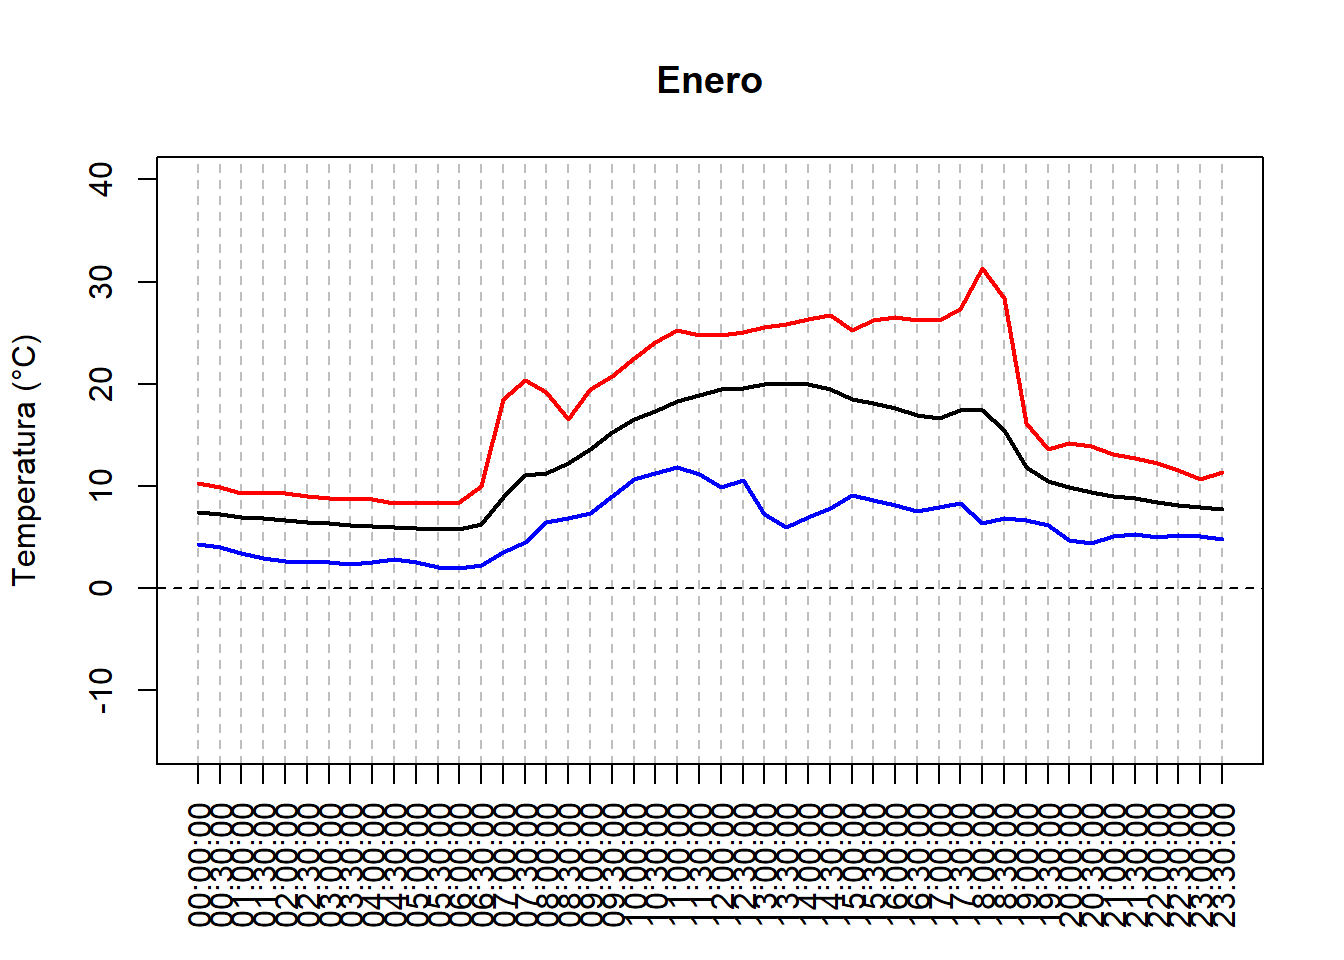
\includegraphics{myRBook_SP_files/figure-latex/unnamed-chunk-251-1.pdf}

\begin{Shaded}
\begin{Highlighting}[]
\KeywordTok{boxplot}\NormalTok{(}\KeywordTok{matrix}\NormalTok{(}\KeywordTok{rnorm}\NormalTok{(}\DecValTok{1000}\NormalTok{), }\DataTypeTok{ncol =} \DecValTok{10}\NormalTok{), }
  \DataTypeTok{col =} \KeywordTok{brewer.pal}\NormalTok{(}\DecValTok{10}\NormalTok{, }\StringTok{"Paired"}\NormalTok{), }\DataTypeTok{axes =} \OtherTok{FALSE}\NormalTok{)}
\end{Highlighting}
\end{Shaded}

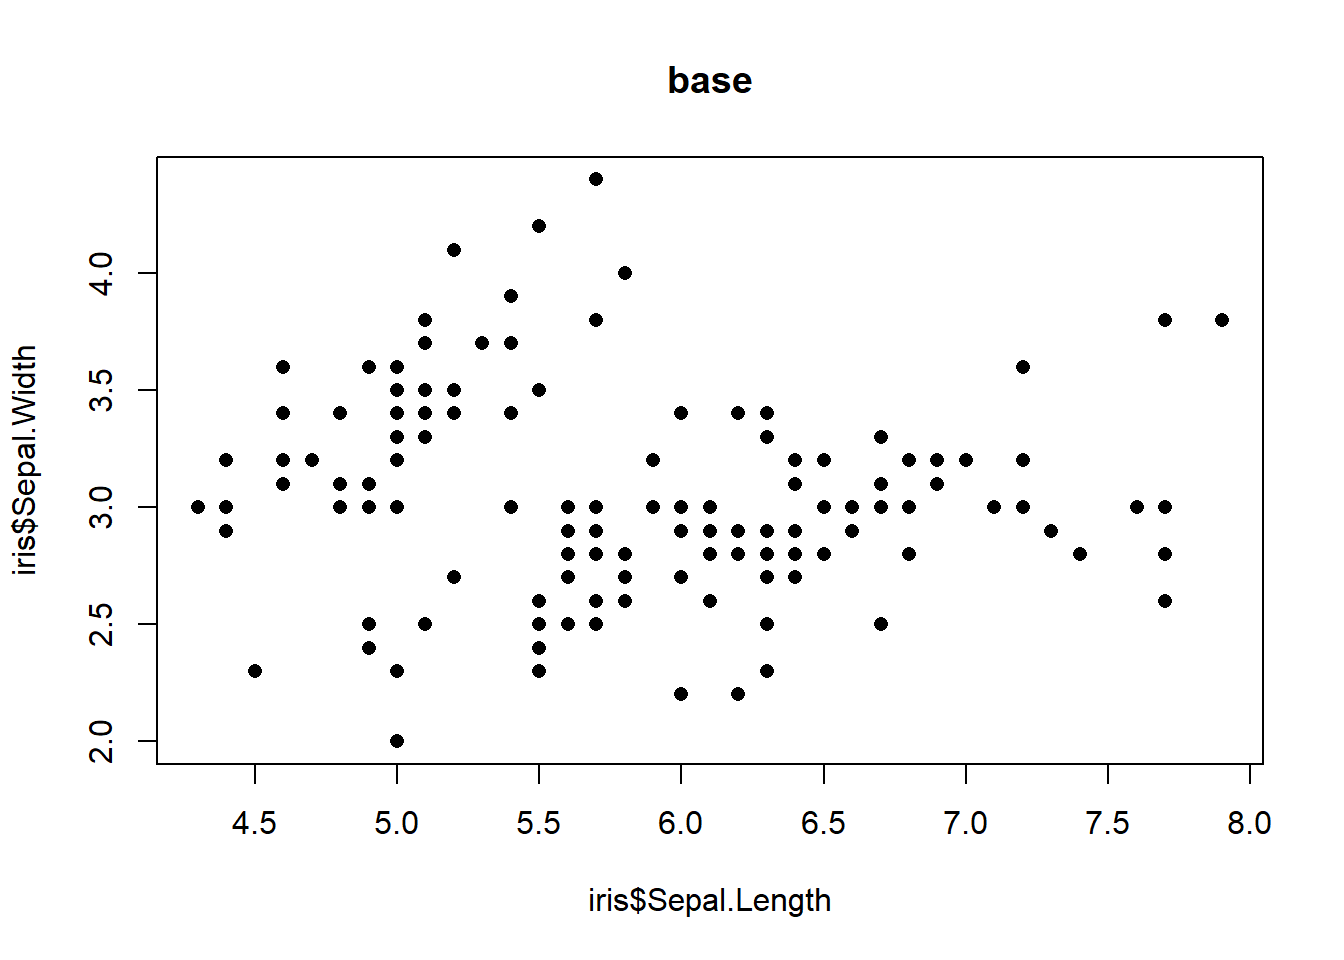
\includegraphics{myRBook_SP_files/figure-latex/unnamed-chunk-251-2.pdf}

\subsection{\texorpdfstring{\texttt{palettesForR}}{palettesForR}}\label{palettesforr}

El paquete \texttt{palettesForR} es otro paquete que contiene paletas
listas para usar de los proyectos `Gimp' y `Inkscape'. Una vez que el
paquete está instalado, solo llamamos a las paletas para utilizarlas.
Las muchas paletas disponibles se enumeran en la ayuda del paquete (hay
48 paletas). Aquí hay un ejemplo de uso.

\begin{Shaded}
\begin{Highlighting}[]
\NormalTok{pkgCheck <-}\StringTok{ }\ControlFlowTok{function}\NormalTok{(x)\{ }
    \ControlFlowTok{if}\NormalTok{ (}\OperatorTok{!}\KeywordTok{require}\NormalTok{(x, }\DataTypeTok{character.only =} \OtherTok{TRUE}\NormalTok{))\{}
        \KeywordTok{install.packages}\NormalTok{(x, }\DataTypeTok{dependencies =} \OtherTok{TRUE}\NormalTok{)}
        \ControlFlowTok{if}\NormalTok{(}\OperatorTok{!}\KeywordTok{require}\NormalTok{(x, }\DataTypeTok{character.only =} \OtherTok{TRUE}\NormalTok{)) \{}
            \KeywordTok{stop}\NormalTok{()}
\NormalTok{        \}}
\NormalTok{    \}}
\NormalTok{\}}
\KeywordTok{pkgCheck}\NormalTok{(}\StringTok{"palettesForR"}\NormalTok{)}
\KeywordTok{showPalette}\NormalTok{(Echo_gpl)}
\end{Highlighting}
\end{Shaded}

\includegraphics{myRBook_SP_files/figure-latex/unnamed-chunk-252-1.pdf}

\begin{Shaded}
\begin{Highlighting}[]
\NormalTok{groupTest <-}\StringTok{ }\KeywordTok{sample}\NormalTok{(}\DecValTok{1}\OperatorTok{:}\DecValTok{3}\NormalTok{, }\DataTypeTok{size =} \DecValTok{100}\NormalTok{, }\DataTypeTok{replace =} \OtherTok{TRUE}\NormalTok{) }
\NormalTok{valueTest <-}\StringTok{ }\KeywordTok{sample}\NormalTok{(}\DecValTok{1}\OperatorTok{:}\DecValTok{7}\NormalTok{, }\DataTypeTok{size =} \DecValTok{100}\NormalTok{, }\DataTypeTok{replace =} \OtherTok{TRUE}\NormalTok{)}
\NormalTok{tableTest <-}\StringTok{ }\KeywordTok{table}\NormalTok{(groupTest, valueTest)}
\KeywordTok{barplot}\NormalTok{(tableTest, }
  \DataTypeTok{col =}\NormalTok{ Echo_gpl, }\DataTypeTok{axes =} \OtherTok{FALSE}\NormalTok{, }\DataTypeTok{beside =} \OtherTok{TRUE}\NormalTok{)}
\end{Highlighting}
\end{Shaded}

\includegraphics{myRBook_SP_files/figure-latex/unnamed-chunk-252-2.pdf}

\begin{Shaded}
\begin{Highlighting}[]
\NormalTok{groupTest <-}\StringTok{ }\KeywordTok{sample}\NormalTok{(}\DecValTok{1}\OperatorTok{:}\DecValTok{3}\NormalTok{, }\DataTypeTok{size =} \DecValTok{100}\NormalTok{, }\DataTypeTok{replace =} \OtherTok{TRUE}\NormalTok{) }
\NormalTok{valueTest <-}\StringTok{ }\KeywordTok{sample}\NormalTok{(}\DecValTok{1}\OperatorTok{:}\DecValTok{7}\NormalTok{, }\DataTypeTok{size =} \DecValTok{100}\NormalTok{, }\DataTypeTok{replace =} \OtherTok{TRUE}\NormalTok{)}
\NormalTok{tableTest <-}\StringTok{ }\KeywordTok{table}\NormalTok{(groupTest, valueTest)}
\KeywordTok{barplot}\NormalTok{(tableTest, }
  \DataTypeTok{col =}\NormalTok{ Tango_gpl, }\DataTypeTok{axes =} \OtherTok{FALSE}\NormalTok{, }\DataTypeTok{beside =} \OtherTok{TRUE}\NormalTok{)}
\end{Highlighting}
\end{Shaded}

\includegraphics{myRBook_SP_files/figure-latex/unnamed-chunk-252-3.pdf}

\subsection{Otros paquetes}\label{otros-paquetes}

Hay muchos paquetes que contienen paletas. Por ejemplo :

\begin{itemize}
\tightlist
\item
  \texttt{viridis} (\url{https://CRAN.R-project.org/package=viridis})
\item
  \texttt{jcolors} (\url{https://CRAN.R-project.org/package=jcolors})
\item
  \texttt{scico} (\url{https://CRAN.R-project.org/package=scico})
\item
  \ldots{}
\end{itemize}

\section{ggplot2 package}\label{ggplot2-package}

El paquete \texttt{ggplot2} es una alternativa a las funciones básicas
de R para realizar gráficos. Se basa en ``La Gramática de Gráficos''
Leland Wilkinson y permite gráficos en capas, por lo general con un
resultado superior si consideramos el aspecto estético en comparacion
con las funciones básicas de R. Si para explorar un conjunto de datos
\texttt{ggplot2} es a veces más potente, nuestros gráficos nunca vienen
solas y se acompañan de análisis estadísticos que a menudo exigen un
trabajo minucioso sobre la gestión de datos. Una vez que nuestras
hipótesis de trabajo estan probadas estadísticamente, resulta fácil
realizar gráficos cual que sea su nivel de complejidad (con las
funciones básicas o con \texttt{ggplot2}). Además veremos en el
siguiente capítulo que desde la gráfica a la figura en el artículo
científico, hay una serie de tratamientos a realizar y el manejo de los
parámetros estéticos se puede hacer de forma independiente de R. Así que
\texttt{ggplot2} es un paquete interesante porque ofrece una alternativa
con una filosofía diferente en la construcción de gráficos, pero no
reemplaza lo que hemos aprendido hasta ahora. En la práctica podemos
utilizar uno u otro en función de los datos y de las manipulaciones que
queremos hacer.

Para volver a \texttt{ggplot2}, empezamos con un ejemplo con los datos
\texttt{iris}.

\begin{Shaded}
\begin{Highlighting}[]
\NormalTok{pkgCheck <-}\StringTok{ }\ControlFlowTok{function}\NormalTok{(x)\{ }
    \ControlFlowTok{if}\NormalTok{ (}\OperatorTok{!}\KeywordTok{require}\NormalTok{(x, }\DataTypeTok{character.only =} \OtherTok{TRUE}\NormalTok{))\{}
        \KeywordTok{install.packages}\NormalTok{(x, }\DataTypeTok{dependencies =} \OtherTok{TRUE}\NormalTok{)}
        \ControlFlowTok{if}\NormalTok{(}\OperatorTok{!}\KeywordTok{require}\NormalTok{(x, }\DataTypeTok{character.only =} \OtherTok{TRUE}\NormalTok{)) \{}
            \KeywordTok{stop}\NormalTok{()}
\NormalTok{        \}}
\NormalTok{    \}}
\NormalTok{\}}
\KeywordTok{pkgCheck}\NormalTok{(}\StringTok{"ggplot2"}\NormalTok{)}
\KeywordTok{data}\NormalTok{(iris)}
\CommentTok{# ggplot2}
\NormalTok{p <-}\StringTok{ }\KeywordTok{ggplot}\NormalTok{(}\DataTypeTok{data =}\NormalTok{ iris, }\KeywordTok{aes}\NormalTok{(}\DataTypeTok{x =}\NormalTok{ Sepal.Length, }\DataTypeTok{y =}\NormalTok{ Sepal.Width))}
\NormalTok{p }\OperatorTok{+}\StringTok{ }\KeywordTok{geom_point}\NormalTok{() }\OperatorTok{+}\StringTok{ }\KeywordTok{ggtitle}\NormalTok{(}\StringTok{"ggplot2"}\NormalTok{)}
\end{Highlighting}
\end{Shaded}

\includegraphics{myRBook_SP_files/figure-latex/unnamed-chunk-253-1.pdf}

\begin{Shaded}
\begin{Highlighting}[]
\CommentTok{# base}
\KeywordTok{plot}\NormalTok{(}\DataTypeTok{x =}\NormalTok{ iris}\OperatorTok{$}\NormalTok{Sepal.Length, }\DataTypeTok{y =}\NormalTok{ iris}\OperatorTok{$}\NormalTok{Sepal.Width, }
  \DataTypeTok{main =} \StringTok{"base"}\NormalTok{, }\DataTypeTok{pch =} \DecValTok{16}\NormalTok{)}
\end{Highlighting}
\end{Shaded}

\includegraphics{myRBook_SP_files/figure-latex/unnamed-chunk-253-2.pdf}

Ahora separemos la información según las especies de flores.

\begin{Shaded}
\begin{Highlighting}[]
\CommentTok{# ggplot2}
\NormalTok{p <-}\StringTok{ }\KeywordTok{ggplot}\NormalTok{(}\DataTypeTok{data =}\NormalTok{ iris, }\KeywordTok{aes}\NormalTok{(}\DataTypeTok{x =}\NormalTok{ Sepal.Length, }\DataTypeTok{y =}\NormalTok{ Sepal.Width, }\DataTypeTok{colour =}\NormalTok{ Species))}
\NormalTok{p }\OperatorTok{+}\StringTok{ }\KeywordTok{geom_point}\NormalTok{() }\OperatorTok{+}\StringTok{ }\KeywordTok{ggtitle}\NormalTok{(}\StringTok{"ggplot2"}\NormalTok{)}
\end{Highlighting}
\end{Shaded}

\includegraphics{myRBook_SP_files/figure-latex/unnamed-chunk-254-1.pdf}

\begin{Shaded}
\begin{Highlighting}[]
\CommentTok{# base}
\KeywordTok{plot}\NormalTok{(}\DataTypeTok{x =}\NormalTok{ iris}\OperatorTok{$}\NormalTok{Sepal.Length, }\DataTypeTok{y =}\NormalTok{ iris}\OperatorTok{$}\NormalTok{Sepal.Width, }
  \DataTypeTok{main =} \StringTok{"base"}\NormalTok{, }\DataTypeTok{pch =} \DecValTok{16}\NormalTok{, }\DataTypeTok{col =}\NormalTok{ iris}\OperatorTok{$}\NormalTok{Species)}
\end{Highlighting}
\end{Shaded}

\includegraphics{myRBook_SP_files/figure-latex/unnamed-chunk-254-2.pdf}

Parece haber una relación entre el ancho y el largo de los sépalos por
especie.

\begin{Shaded}
\begin{Highlighting}[]
\CommentTok{# linear regressions}
\NormalTok{lmFits <-}\StringTok{ }\KeywordTok{lapply}\NormalTok{(}\DecValTok{1}\OperatorTok{:}\DecValTok{3}\NormalTok{, }\ControlFlowTok{function}\NormalTok{(i)\{}
\NormalTok{  fitSp1 <-}\StringTok{ }\KeywordTok{lm}\NormalTok{(iris}\OperatorTok{$}\NormalTok{Sepal.Width[}\KeywordTok{as.numeric}\NormalTok{(iris}\OperatorTok{$}\NormalTok{Species) }\OperatorTok{==}\StringTok{ }\NormalTok{i] }\OperatorTok{~}\StringTok{ }
\StringTok{    }\NormalTok{iris}\OperatorTok{$}\NormalTok{Sepal.Length[}\KeywordTok{as.numeric}\NormalTok{(iris}\OperatorTok{$}\NormalTok{Species) }\OperatorTok{==}\StringTok{ }\NormalTok{i])}
\NormalTok{  fStat1 <-}\StringTok{ }\KeywordTok{summary}\NormalTok{(fitSp1)}\OperatorTok{$}\NormalTok{fstatistic}
\NormalTok{  rSq1 <-}\StringTok{ }\KeywordTok{summary}\NormalTok{(fitSp1)}\OperatorTok{$}\NormalTok{r.squared}
\NormalTok{  pVal1 <-}\StringTok{ }\KeywordTok{summary}\NormalTok{(fitSp1)}\OperatorTok{$}\NormalTok{coefficients[}\DecValTok{2}\NormalTok{, }\DecValTok{4}\NormalTok{]}
\NormalTok{  stat1 <-}\StringTok{ }\KeywordTok{paste0}\NormalTok{(}\StringTok{"F="}\NormalTok{, }\KeywordTok{round}\NormalTok{(fStat1[}\DecValTok{1}\NormalTok{], }\DataTypeTok{digits =} \DecValTok{2}\NormalTok{), }
    \StringTok{"; DF="}\NormalTok{, fStat1[}\DecValTok{2}\NormalTok{], }\StringTok{"/"}\NormalTok{, fStat1[}\DecValTok{3}\NormalTok{], }\StringTok{"; r-sq="}\NormalTok{, }\KeywordTok{round}\NormalTok{(rSq1, }\DataTypeTok{digits =} \DecValTok{2}\NormalTok{), }
    \StringTok{"; p-val="}\NormalTok{, }\KeywordTok{round}\NormalTok{(pVal1, }\DataTypeTok{digits =} \DecValTok{6}\NormalTok{))}
  \KeywordTok{return}\NormalTok{(}\KeywordTok{list}\NormalTok{(fitSp1, stat1))}
\NormalTok{\})}
\CommentTok{# ggplot2}
\NormalTok{p <-}\StringTok{ }\KeywordTok{ggplot}\NormalTok{(}\DataTypeTok{data =}\NormalTok{ iris, }\KeywordTok{aes}\NormalTok{(}\DataTypeTok{x =}\NormalTok{ Sepal.Length, }\DataTypeTok{y =}\NormalTok{ Sepal.Width, }\DataTypeTok{colour =}\NormalTok{ Species))}
\NormalTok{p <-}\StringTok{ }\NormalTok{p }\OperatorTok{+}\StringTok{ }\KeywordTok{geom_point}\NormalTok{() }\OperatorTok{+}\StringTok{ }\KeywordTok{ggtitle}\NormalTok{(}\StringTok{"ggplot2"}\NormalTok{) }\OperatorTok{+}\StringTok{ }\KeywordTok{stat_smooth}\NormalTok{(}\DataTypeTok{method =} \StringTok{"lm"}\NormalTok{, }\DataTypeTok{se =} \OtherTok{FALSE}\NormalTok{)}
\NormalTok{p <-}\StringTok{ }\NormalTok{p }\OperatorTok{+}\StringTok{ }\KeywordTok{annotate}\NormalTok{(}\DataTypeTok{geom =} \StringTok{"text"}\NormalTok{, }\DataTypeTok{x =} \DecValTok{6}\NormalTok{, }\DataTypeTok{y =} \FloatTok{2.250}\NormalTok{, }\DataTypeTok{label =}\NormalTok{ lmFits[[}\DecValTok{1}\NormalTok{]][[}\DecValTok{2}\NormalTok{]], }\DataTypeTok{colour =} \DecValTok{2}\NormalTok{)}
\NormalTok{p <-}\StringTok{ }\NormalTok{p }\OperatorTok{+}\StringTok{ }\KeywordTok{annotate}\NormalTok{(}\DataTypeTok{geom =} \StringTok{"text"}\NormalTok{, }\DataTypeTok{x =} \DecValTok{6}\NormalTok{, }\DataTypeTok{y =} \FloatTok{2.125}\NormalTok{, }\DataTypeTok{label =}\NormalTok{ lmFits[[}\DecValTok{2}\NormalTok{]][[}\DecValTok{2}\NormalTok{]], }\DataTypeTok{colour =} \DecValTok{3}\NormalTok{)}
\NormalTok{p <-}\StringTok{ }\NormalTok{p }\OperatorTok{+}\StringTok{ }\KeywordTok{annotate}\NormalTok{(}\DataTypeTok{geom =} \StringTok{"text"}\NormalTok{, }\DataTypeTok{x =} \DecValTok{6}\NormalTok{, }\DataTypeTok{y =} \FloatTok{2.000}\NormalTok{, }\DataTypeTok{label =}\NormalTok{ lmFits[[}\DecValTok{3}\NormalTok{]][[}\DecValTok{2}\NormalTok{]], }\DataTypeTok{colour =} \DecValTok{4}\NormalTok{)}
\NormalTok{p}
\end{Highlighting}
\end{Shaded}

\includegraphics{myRBook_SP_files/figure-latex/unnamed-chunk-255-1.pdf}

\begin{Shaded}
\begin{Highlighting}[]
\CommentTok{# base}
\KeywordTok{plot}\NormalTok{(}\DataTypeTok{x =}\NormalTok{ iris}\OperatorTok{$}\NormalTok{Sepal.Length, }\DataTypeTok{y =}\NormalTok{ iris}\OperatorTok{$}\NormalTok{Sepal.Width, }
  \DataTypeTok{main =} \StringTok{"base"}\NormalTok{, }\DataTypeTok{pch =} \DecValTok{16}\NormalTok{, }\DataTypeTok{col =}\NormalTok{ iris}\OperatorTok{$}\NormalTok{Species)}
\KeywordTok{abline}\NormalTok{(lmFits[[}\DecValTok{1}\NormalTok{]][[}\DecValTok{1}\NormalTok{]], }\DataTypeTok{col =} \DecValTok{1}\NormalTok{)}
\KeywordTok{abline}\NormalTok{(lmFits[[}\DecValTok{2}\NormalTok{]][[}\DecValTok{1}\NormalTok{]], }\DataTypeTok{col =} \DecValTok{2}\NormalTok{)}
\KeywordTok{abline}\NormalTok{(lmFits[[}\DecValTok{3}\NormalTok{]][[}\DecValTok{1}\NormalTok{]], }\DataTypeTok{col =} \DecValTok{3}\NormalTok{)}
\KeywordTok{text}\NormalTok{(}\DataTypeTok{x =} \FloatTok{5.5}\NormalTok{, }\DataTypeTok{y =} \FloatTok{2.2}\NormalTok{, }\DataTypeTok{labels =}\NormalTok{ lmFits[[}\DecValTok{1}\NormalTok{]][[}\DecValTok{2}\NormalTok{]], }\DataTypeTok{pos =} \DecValTok{4}\NormalTok{)}
\KeywordTok{text}\NormalTok{(}\DataTypeTok{x =} \FloatTok{5.5}\NormalTok{, }\DataTypeTok{y =} \FloatTok{2.1}\NormalTok{, }\DataTypeTok{labels =}\NormalTok{ lmFits[[}\DecValTok{2}\NormalTok{]][[}\DecValTok{2}\NormalTok{]], }\DataTypeTok{pos =} \DecValTok{4}\NormalTok{, }\DataTypeTok{col =} \DecValTok{2}\NormalTok{)}
\KeywordTok{text}\NormalTok{(}\DataTypeTok{x =} \FloatTok{5.5}\NormalTok{, }\DataTypeTok{y =} \FloatTok{2.0}\NormalTok{, }\DataTypeTok{labels =}\NormalTok{ lmFits[[}\DecValTok{3}\NormalTok{]][[}\DecValTok{2}\NormalTok{]], }\DataTypeTok{pos =} \DecValTok{4}\NormalTok{, }\DataTypeTok{col =} \DecValTok{3}\NormalTok{)}
\end{Highlighting}
\end{Shaded}

\includegraphics{myRBook_SP_files/figure-latex/unnamed-chunk-255-2.pdf}

Podemos ver en estos ejemplos que los gráficos con \texttt{ggplot2}
comienzan con una llamada a la función \texttt{ggplot()}, en la cual el
primer argumento \texttt{datos} coincide con nuestros datos
(generalmente un \texttt{data.frame}), y El segundo argumento
\texttt{aes()} es la información que queremos usar. Por convención, esta
información se almacena en un objeto \texttt{p}. Luego agregaremos capas
adicionales usando \texttt{+}.

En las capas podemos agregar aspectos geométricos (el tipo de gráfico,
por ejemplo, \texttt{geom\_point()}), estadísticas (por ejemplo,
\texttt{stat\_smooth()}), anotaciones (por ejemplo,
\texttt{annotate()}), y otras cosas relacionadas con los ejes, los
colores, \ldots{} La documentación completa se puede consultar en la
dirección \url{https://ggplot2.tidyverse.org/} (hoja de resumen:
\url{https://github.com/rstudio/cheatsheets/blob/master/data-visualization-2.1.pdf}).
Muchas extensiones a \texttt{ggplot2} están disponibles en
\url{http://www.ggplot2-exts.org/gallery/}.

\section{\texorpdfstring{Gráficos interactivos y dinámicos con
\texttt{Plotly}}{Gráficos interactivos y dinámicos con Plotly}}\label{graficos-interactivos-y-dinamicos-con-plotly}

\texttt{Plotly} es un paquete para gráficos interactivos y dinámicos.
Esto puede ser particularmente útil para los resultados que se difunden
a través de Internet. El paquete se instala como cualquier otro con
\texttt{install.packages("plotly")}. El paquete es gratuito y de código
abierto.

Este ejemplo se ha copiado del libro de Carson Sievert
(\url{https://plotly-book.cpsievert.me}). El código usado para hacer
este gráfico está licenciado bajo la licencia de Estados Unidos Creative
Commons Attribution-NonCommercial-NoDerivs 3.0 (Carson Sievert;
\url{https://creativecommons.org/licenses/by-nc-nd/3.0/us/}).

\includegraphics{myRBook_SP_files/figure-latex/unnamed-chunk-256-1.pdf}

\section{Conclusión}\label{conclusion-10}

Este capítulo nos permitió ver otras opciones gráficas y, en particular,
los paquetes \texttt{ggplot2} y \texttt{plotly}. Existen libros
específicos (en inglés) que cubren todos los aspectos de estos paquetes,
aquí el objetivo es saber que existen estas opciones para usarlos si es
necesario. Los sitios web ``Data to Viz'' y ``r-graph gallery''
(\url{https://www.data-to-viz.com};
\url{https://www.r-graph-gallery.com/}) son buenos recursos para tener
ideas de las posibilidades que ofrece R en cuanto a representaciones
gráficas. El siguiente capítulo analiza los procesos necesarios para
transformar un gráfico R en una figura publicable en un artículo
científico. Hasta muy pronto !

\part{Estudio de caso}\label{part-estudio-de-caso}

\hypertarget{studyCase1}{\chapter{Analizar datos de loggers de
temperatura}\label{studyCase1}}

En estudios de biología, ecología, o agronomía, frecuentemente usamos
datos de temperatura de dataloggers. En este estudio vamos a ver como
analizar esos datos usando datos de temperatura del altiplano Boliviano
cerca de la ciudad de El Alto. El primer paso es transformar los datos
del datalogger en un formato que sea fácil de leer para R. Usaremos un
archivo CSV y la función
\protect\hyperlink{import}{\texttt{read.table()}}. El archivo se puede
descargar desde el sitio web del libro en GitHub
(\url{https://github.com/frareb/myRBook_SP/blob/master/myFiles/E05C13.csv}
; clic derecho sobre el enlace y seleccionar ``Guardar destino como'').

\begin{Shaded}
\begin{Highlighting}[]
\NormalTok{bdd <-}\StringTok{ }\KeywordTok{read.table}\NormalTok{(}\StringTok{"myFiles/E05C13.csv"}\NormalTok{, }\DataTypeTok{skip =} \DecValTok{1}\NormalTok{, }\DataTypeTok{header =} \OtherTok{TRUE}\NormalTok{, }
  \DataTypeTok{sep =} \StringTok{","}\NormalTok{, }\DataTypeTok{dec =} \StringTok{"."}\NormalTok{, }\DataTypeTok{stringsAsFactors =} \OtherTok{FALSE}\NormalTok{)}
\KeywordTok{colnames}\NormalTok{(bdd) <-}\StringTok{ }\KeywordTok{c}\NormalTok{(}\StringTok{"id"}\NormalTok{, }\StringTok{"date"}\NormalTok{, }\StringTok{"temp"}\NormalTok{)}
\KeywordTok{head}\NormalTok{(bdd)}
\end{Highlighting}
\end{Shaded}

\begin{verbatim}
##   id              date  temp
## 1  1 11/12/15 23:00:00 4.973
## 2  2 11/12/15 23:30:00 4.766
## 3  3 11/13/15 00:00:00 4.844
## 4  4 11/13/15 00:30:00 4.844
## 5  5 11/13/15 01:00:00 5.076
## 6  6 11/13/15 01:30:00 5.282
\end{verbatim}

\begin{Shaded}
\begin{Highlighting}[]
\KeywordTok{tail}\NormalTok{(bdd)}
\end{Highlighting}
\end{Shaded}

\begin{verbatim}
##          id              date  temp
## 32781 32781 09/25/17 21:00:00 7.091
## 32782 32782 09/25/17 21:30:00 6.914
## 32783 32783 09/25/17 22:00:00 6.813
## 32784 32784 09/25/17 22:30:00 6.611
## 32785 32785 09/25/17 23:00:00 6.331
## 32786 32786 09/25/17 23:30:00 5.385
\end{verbatim}

\begin{Shaded}
\begin{Highlighting}[]
\KeywordTok{str}\NormalTok{(bdd)}
\end{Highlighting}
\end{Shaded}

\begin{verbatim}
## 'data.frame':    32786 obs. of  3 variables:
##  $ id  : int  1 2 3 4 5 6 7 8 9 10 ...
##  $ date: chr  "11/12/15 23:00:00" "11/12/15 23:30:00" "11/13/15 00:00:00" "11/13/15 00:30:00" ...
##  $ temp: num  4.97 4.77 4.84 4.84 5.08 ...
\end{verbatim}

Podemos observar que la fecha esta al formato \texttt{character}, y que
contiene la fecha con el mes, el día, y el año separados con \texttt{/},
un espacio, y la hora con horas de 0 a 24, minutos, y segundos,
separados con \texttt{:} (ejemplo: \texttt{11/12/15\ 23:00:00} para el
12 de Noviembre de 2015 a las 11 de la noche). Vamos a separar la
información en varios objetos. Primero vamos a separar la fecha de la
hora. Para esto vamos a usar la función \texttt{strsplit()} usando como
separador el espacio entre la fecha y la hora.

\begin{Shaded}
\begin{Highlighting}[]
\KeywordTok{strsplit}\NormalTok{(}\StringTok{"11/12/15 23:00:00"}\NormalTok{, }\DataTypeTok{split =} \StringTok{" "}\NormalTok{)}
\end{Highlighting}
\end{Shaded}

\begin{verbatim}
## [[1]]
## [1] "11/12/15" "23:00:00"
\end{verbatim}

Como indican los corchetes dobles, la función devuelve un objeto en el
formato \texttt{list}. Nosotros queremos el \texttt{vector} que
corresponde al primer elemento de la \texttt{list} entonces vamos a
añadir \texttt{{[}{[}1{]}{]}}.

\begin{Shaded}
\begin{Highlighting}[]
\KeywordTok{strsplit}\NormalTok{(}\StringTok{"11/12/15 23:00:00"}\NormalTok{, }\DataTypeTok{split =} \StringTok{" "}\NormalTok{)[[}\DecValTok{1}\NormalTok{]]}
\end{Highlighting}
\end{Shaded}

\begin{verbatim}
## [1] "11/12/15" "23:00:00"
\end{verbatim}

El primer elemento del \texttt{vector} es la fecha. Para tener todas las
fechas vamos a hacer un bucle con la función \texttt{sapply()}.

\begin{Shaded}
\begin{Highlighting}[]
\NormalTok{bddDay <-}\StringTok{ }\KeywordTok{sapply}\NormalTok{(}\KeywordTok{strsplit}\NormalTok{(bdd[, }\DecValTok{2}\NormalTok{], }\DataTypeTok{split =} \StringTok{" "}\NormalTok{), }\StringTok{"[["}\NormalTok{, }\DecValTok{1}\NormalTok{)}
\KeywordTok{head}\NormalTok{(bddDay)}
\end{Highlighting}
\end{Shaded}

\begin{verbatim}
## [1] "11/12/15" "11/12/15" "11/13/15" "11/13/15" "11/13/15" "11/13/15"
\end{verbatim}

A continuación vamos a necesitar las fechas en el formato
\texttt{factor} (función \texttt{aggregate()} para sacar la información
por día). Entonces necesitamos transformar el objeto en el formato
\texttt{factor} con la función \texttt{as.factor()}.

\begin{Shaded}
\begin{Highlighting}[]
\NormalTok{bddDay <-}\StringTok{ }\KeywordTok{as.factor}\NormalTok{(}\KeywordTok{sapply}\NormalTok{(}\KeywordTok{strsplit}\NormalTok{(bdd[, }\DecValTok{2}\NormalTok{], }\DataTypeTok{split =} \StringTok{" "}\NormalTok{), }\StringTok{"[["}\NormalTok{, }\DecValTok{1}\NormalTok{))}
\KeywordTok{head}\NormalTok{(bddDay)}
\end{Highlighting}
\end{Shaded}

\begin{verbatim}
## [1] 11/12/15 11/12/15 11/13/15 11/13/15 11/13/15 11/13/15
## 684 Levels: 01/01/16 01/01/17 01/02/16 01/02/17 01/03/16 ... 12/31/16
\end{verbatim}

Haciendo la transformación hacia el formato \texttt{factor}, los niveles
de nuestro objeto están en orden alfabético como si las fechas
estuvieran texto. Nosotros querremos ordenar las fechas usando las
fechas. Para esto vamos a hacer un \texttt{vector} con todas las fechas
únicas con la función \texttt{unique()}, y después ordenar las fechas
con la función \texttt{sort.list()} usando las fechas con la función
\texttt{as.POSIXct()}. Vamos a usar el vector llamado \texttt{lev} para
especificar como deben estar los niveles de \texttt{factor} de nuestras
fechas.

\begin{Shaded}
\begin{Highlighting}[]
\NormalTok{bddDay <-}\StringTok{ }\KeywordTok{as.factor}\NormalTok{(}\KeywordTok{sapply}\NormalTok{(}\KeywordTok{strsplit}\NormalTok{(bdd[, }\DecValTok{2}\NormalTok{], }\DataTypeTok{split =} \StringTok{" "}\NormalTok{), }\StringTok{"[["}\NormalTok{, }\DecValTok{1}\NormalTok{))}
\NormalTok{udate <-}\StringTok{ }\KeywordTok{unique}\NormalTok{(bddDay)}
\NormalTok{lev <-}\StringTok{ }\NormalTok{udate[}\KeywordTok{sort.list}\NormalTok{(}\KeywordTok{as.POSIXct}\NormalTok{(}\KeywordTok{strptime}\NormalTok{(udate, }\StringTok{"%m/%d/%y"}\NormalTok{)))]}
\NormalTok{bddDay <-}\StringTok{ }\KeywordTok{factor}\NormalTok{(bddDay, }\DataTypeTok{levels =}\NormalTok{ lev)}
\KeywordTok{head}\NormalTok{(bddDay)}
\end{Highlighting}
\end{Shaded}

\begin{verbatim}
## [1] 11/12/15 11/12/15 11/13/15 11/13/15 11/13/15 11/13/15
## 684 Levels: 11/12/15 11/13/15 11/14/15 11/15/15 11/16/15 ... 09/25/17
\end{verbatim}

Ahora podemos añadir las fechas como nueva columna del objeto
\texttt{bdd} y hacer lo mismo para las horas (no hay que reordenar los
niveles de hora ya que el orden por defecto corresponde a lo que
queremos).

\begin{Shaded}
\begin{Highlighting}[]
\NormalTok{bdd}\OperatorTok{$}\NormalTok{bddDay <-}\StringTok{ }\NormalTok{bddDay}
\NormalTok{bdd}\OperatorTok{$}\NormalTok{bddHour <-}\StringTok{ }\KeywordTok{as.factor}\NormalTok{(}\KeywordTok{sapply}\NormalTok{(}\KeywordTok{strsplit}\NormalTok{(bdd[, }\DecValTok{2}\NormalTok{], }\DataTypeTok{split =} \StringTok{" "}\NormalTok{), }\StringTok{"[["}\NormalTok{, }\DecValTok{2}\NormalTok{))}
\KeywordTok{head}\NormalTok{(bdd)}
\end{Highlighting}
\end{Shaded}

\begin{verbatim}
##   id              date  temp   bddDay  bddHour
## 1  1 11/12/15 23:00:00 4.973 11/12/15 23:00:00
## 2  2 11/12/15 23:30:00 4.766 11/12/15 23:30:00
## 3  3 11/13/15 00:00:00 4.844 11/13/15 00:00:00
## 4  4 11/13/15 00:30:00 4.844 11/13/15 00:30:00
## 5  5 11/13/15 01:00:00 5.076 11/13/15 01:00:00
## 6  6 11/13/15 01:30:00 5.282 11/13/15 01:30:00
\end{verbatim}

Podemos visualizar los datos con la función \texttt{plot()},
especificando el formato de las fechas con la función \texttt{as.Date()}

\begin{Shaded}
\begin{Highlighting}[]
\KeywordTok{plot}\NormalTok{(}\DataTypeTok{x =} \KeywordTok{as.Date}\NormalTok{(bdd}\OperatorTok{$}\NormalTok{bddDay, }\DataTypeTok{format =} \StringTok{"%m/%d/%y"}\NormalTok{), }\DataTypeTok{y =}\NormalTok{ bdd}\OperatorTok{$}\NormalTok{temp, }
    \DataTypeTok{type =} \StringTok{'l'}\NormalTok{, }\DataTypeTok{ylim =} \KeywordTok{c}\NormalTok{(}\OperatorTok{-}\DecValTok{15}\NormalTok{, }\DecValTok{40}\NormalTok{), }
    \DataTypeTok{xlab =} \StringTok{"Fecha"}\NormalTok{, }\DataTypeTok{ylab =} \StringTok{"Temperatura (°C)"}\NormalTok{)}
\end{Highlighting}
\end{Shaded}

\includegraphics{myRBook_SP_files/figure-latex/unnamed-chunk-264-1.pdf}

Podemos simplificar la información calculando únicamente las
temperaturas mínimas, promedias, y máximas con la función
\texttt{aggregate()}.

\begin{Shaded}
\begin{Highlighting}[]
\NormalTok{tempDayMean <-}\StringTok{ }\KeywordTok{aggregate}\NormalTok{(}\DataTypeTok{x =}\NormalTok{ bdd[, }\DecValTok{3}\NormalTok{], }\DataTypeTok{by =} \KeywordTok{list}\NormalTok{(bdd[, }\DecValTok{4}\NormalTok{]), }\DataTypeTok{FUN =}\NormalTok{ mean)}
\NormalTok{tempDayMin <-}\StringTok{ }\KeywordTok{aggregate}\NormalTok{(}\DataTypeTok{x =}\NormalTok{ bdd[, }\DecValTok{3}\NormalTok{], }\DataTypeTok{by =} \KeywordTok{list}\NormalTok{(bdd[, }\DecValTok{4}\NormalTok{]), }\DataTypeTok{FUN =}\NormalTok{ min)}
\NormalTok{tempDayMax <-}\StringTok{ }\KeywordTok{aggregate}\NormalTok{(}\DataTypeTok{x =}\NormalTok{ bdd[, }\DecValTok{3}\NormalTok{], }\DataTypeTok{by =} \KeywordTok{list}\NormalTok{(bdd[, }\DecValTok{4}\NormalTok{]), }\DataTypeTok{FUN =}\NormalTok{ max)}
\KeywordTok{plot}\NormalTok{(}\DataTypeTok{x =} \KeywordTok{as.Date}\NormalTok{(tempDayMean[, }\DecValTok{1}\NormalTok{], }\DataTypeTok{format =} \StringTok{"%m/%d/%y"}\NormalTok{), }
    \DataTypeTok{y =}\NormalTok{ tempDayMean[, }\DecValTok{2}\NormalTok{], }\DataTypeTok{type =} \StringTok{'l'}\NormalTok{, }\DataTypeTok{ylim =} \KeywordTok{c}\NormalTok{(}\OperatorTok{-}\DecValTok{15}\NormalTok{, }\DecValTok{40}\NormalTok{), }
    \DataTypeTok{xlab =} \StringTok{"Fecha"}\NormalTok{, }\DataTypeTok{ylab =} \StringTok{"Temperatura (°C)"}\NormalTok{)}
\KeywordTok{points}\NormalTok{(}\DataTypeTok{x =} \KeywordTok{as.Date}\NormalTok{(tempDayMin[, }\DecValTok{1}\NormalTok{], }\DataTypeTok{format =} \StringTok{"%m/%d/%y"}\NormalTok{), }
    \DataTypeTok{y =}\NormalTok{ tempDayMin[, }\DecValTok{2}\NormalTok{], }\DataTypeTok{type =} \StringTok{'l'}\NormalTok{, }\DataTypeTok{col =} \DecValTok{4}\NormalTok{)}
\KeywordTok{points}\NormalTok{(}\DataTypeTok{x =} \KeywordTok{as.Date}\NormalTok{(tempDayMax[, }\DecValTok{1}\NormalTok{], }\DataTypeTok{format =} \StringTok{"%m/%d/%y"}\NormalTok{), }
    \DataTypeTok{y =}\NormalTok{ tempDayMax[, }\DecValTok{2}\NormalTok{], }\DataTypeTok{type =} \StringTok{'l'}\NormalTok{, }\DataTypeTok{col =} \DecValTok{2}\NormalTok{)}
\KeywordTok{legend}\NormalTok{(}\StringTok{"topright"}\NormalTok{, }\DataTypeTok{legend =} \KeywordTok{c}\NormalTok{(}\StringTok{"min"}\NormalTok{, }\StringTok{"max"}\NormalTok{, }\StringTok{"promedio"}\NormalTok{), }
  \DataTypeTok{lty =} \DecValTok{1}\NormalTok{, }\DataTypeTok{lwd =} \DecValTok{2}\NormalTok{, }\DataTypeTok{col =} \KeywordTok{c}\NormalTok{(}\DecValTok{4}\NormalTok{, }\DecValTok{2}\NormalTok{, }\DecValTok{1}\NormalTok{))}
\end{Highlighting}
\end{Shaded}

\includegraphics{myRBook_SP_files/figure-latex/unnamed-chunk-265-1.pdf}

También podemos calcular la diferencia entre la temperatura máxima y la
temperatura mínima (variación de temperatura diurna).

\begin{Shaded}
\begin{Highlighting}[]
\NormalTok{tempDayTR <-}\StringTok{ }\NormalTok{tempDayMax[, }\DecValTok{2}\NormalTok{] }\OperatorTok{-}\StringTok{ }\NormalTok{tempDayMin[, }\DecValTok{2}\NormalTok{]}
\KeywordTok{plot}\NormalTok{(}\DataTypeTok{x =} \KeywordTok{as.Date}\NormalTok{(tempDayMean[, }\DecValTok{1}\NormalTok{], }\DataTypeTok{format =} \StringTok{"%m/%d/%y"}\NormalTok{), }
    \DataTypeTok{y =}\NormalTok{ tempDayTR, }\DataTypeTok{type =} \StringTok{'l'}\NormalTok{, }\DataTypeTok{ylim =} \KeywordTok{c}\NormalTok{(}\DecValTok{5}\NormalTok{, }\DecValTok{45}\NormalTok{), }
    \DataTypeTok{xlab =} \StringTok{"Fecha"}\NormalTok{, }\DataTypeTok{ylab =} \StringTok{"Variación de temperatura diurna (°C)"}\NormalTok{)}
\end{Highlighting}
\end{Shaded}

\includegraphics{myRBook_SP_files/figure-latex/unnamed-chunk-266-1.pdf}

Otra posibilidad es de agrupar los datos para tener la temperatura
promedia de un día con la función \texttt{aggregate()}.

\begin{Shaded}
\begin{Highlighting}[]
\NormalTok{tempHourMean <-}\StringTok{ }\KeywordTok{aggregate}\NormalTok{(}\DataTypeTok{x =}\NormalTok{ bdd[, }\DecValTok{3}\NormalTok{], }\DataTypeTok{by =} \KeywordTok{list}\NormalTok{(bdd[, }\DecValTok{5}\NormalTok{]), }\DataTypeTok{FUN =}\NormalTok{ mean)}
\NormalTok{tempHourMin <-}\StringTok{ }\KeywordTok{aggregate}\NormalTok{(}\DataTypeTok{x =}\NormalTok{ bdd[, }\DecValTok{3}\NormalTok{], }\DataTypeTok{by =} \KeywordTok{list}\NormalTok{(bdd[, }\DecValTok{5}\NormalTok{]), }\DataTypeTok{FUN =}\NormalTok{ min)}
\NormalTok{tempHourMax <-}\StringTok{ }\KeywordTok{aggregate}\NormalTok{(}\DataTypeTok{x =}\NormalTok{ bdd[, }\DecValTok{3}\NormalTok{], }\DataTypeTok{by =} \KeywordTok{list}\NormalTok{(bdd[, }\DecValTok{5}\NormalTok{]), }\DataTypeTok{FUN =}\NormalTok{ max)}
\NormalTok{hours <-}\StringTok{ }\KeywordTok{seq}\NormalTok{(}\DataTypeTok{from =} \DecValTok{0}\NormalTok{, }\DataTypeTok{to =} \FloatTok{23.5}\NormalTok{, }\DataTypeTok{by =} \FloatTok{0.5}\NormalTok{)}
\KeywordTok{plot}\NormalTok{(}\DataTypeTok{x =}\NormalTok{ hours, }
    \DataTypeTok{y =}\NormalTok{ tempHourMean[, }\DecValTok{2}\NormalTok{], }\DataTypeTok{type =} \StringTok{'l'}\NormalTok{, }\DataTypeTok{ylim =} \KeywordTok{c}\NormalTok{(}\OperatorTok{-}\DecValTok{15}\NormalTok{, }\DecValTok{40}\NormalTok{), }
    \DataTypeTok{xlab =} \StringTok{""}\NormalTok{, }\DataTypeTok{ylab =} \StringTok{"Temperatura (°C)"}\NormalTok{, }\DataTypeTok{lwd =} \DecValTok{2}\NormalTok{, }
    \DataTypeTok{xaxt =} \StringTok{"n"}\NormalTok{, }\DataTypeTok{panel.first =}\NormalTok{ \{}
        \KeywordTok{abline}\NormalTok{(}\DataTypeTok{v =}\NormalTok{ hours, }\DataTypeTok{col =} \StringTok{"gray"}\NormalTok{, }\DataTypeTok{lty =} \DecValTok{2}\NormalTok{)}
        \KeywordTok{abline}\NormalTok{(}\DataTypeTok{h =} \DecValTok{0}\NormalTok{, }\DataTypeTok{lty =} \DecValTok{2}\NormalTok{)  }
\NormalTok{    \})}
\KeywordTok{axis}\NormalTok{(}\DataTypeTok{side =} \DecValTok{1}\NormalTok{, }\DataTypeTok{at =}\NormalTok{ hours, }\DataTypeTok{labels =}\NormalTok{ tempHourMean[, }\DecValTok{1}\NormalTok{], }\DataTypeTok{las =} \DecValTok{2}\NormalTok{)}
\KeywordTok{points}\NormalTok{(}\DataTypeTok{x =}\NormalTok{ hours, }\DataTypeTok{y =}\NormalTok{ tempHourMin[, }\DecValTok{2}\NormalTok{], }\DataTypeTok{type =} \StringTok{'l'}\NormalTok{, }\DataTypeTok{col =} \DecValTok{4}\NormalTok{, }\DataTypeTok{lwd =} \DecValTok{2}\NormalTok{)}
\KeywordTok{points}\NormalTok{(}\DataTypeTok{x =}\NormalTok{ hours, }\DataTypeTok{y =}\NormalTok{ tempHourMax[, }\DecValTok{2}\NormalTok{], }\DataTypeTok{type =} \StringTok{'l'}\NormalTok{, }\DataTypeTok{col =} \DecValTok{2}\NormalTok{, }\DataTypeTok{lwd =} \DecValTok{2}\NormalTok{)}
\end{Highlighting}
\end{Shaded}

\includegraphics{myRBook_SP_files/figure-latex/unnamed-chunk-267-1.pdf}

Tambien podemos calcular las temperaturas de los dias para cada mes.

\begin{Shaded}
\begin{Highlighting}[]
\NormalTok{meses <-}\StringTok{ }\KeywordTok{c}\NormalTok{(}\StringTok{"Enero"}\NormalTok{, }\StringTok{"Febrero"}\NormalTok{, }\StringTok{"Marzo"}\NormalTok{, }\StringTok{"Abril"}\NormalTok{, }\StringTok{"Mayo"}\NormalTok{, }\StringTok{"Junio"}\NormalTok{, }
    \StringTok{"Julio"}\NormalTok{, }\StringTok{"Agosto"}\NormalTok{, }\StringTok{"Septiembre"}\NormalTok{, }\StringTok{"Octubre"}\NormalTok{, }\StringTok{"Noviembre"}\NormalTok{, }\StringTok{"Diciembre"}\NormalTok{)}
\NormalTok{hours <-}\StringTok{ }\KeywordTok{seq}\NormalTok{(}\DataTypeTok{from =} \DecValTok{0}\NormalTok{, }\DataTypeTok{to =} \FloatTok{23.5}\NormalTok{, }\DataTypeTok{by =} \FloatTok{0.5}\NormalTok{)}
\NormalTok{bddMonth <-}\StringTok{ }\KeywordTok{sapply}\NormalTok{(}\KeywordTok{strsplit}\NormalTok{(}\KeywordTok{as.character}\NormalTok{(bdd}\OperatorTok{$}\NormalTok{bddDay), }\DataTypeTok{split =} \StringTok{"/"}\NormalTok{), }\StringTok{"[["}\NormalTok{, }\DecValTok{1}\NormalTok{)}
\NormalTok{tempDayEachMonth <-}\StringTok{ }\KeywordTok{lapply}\NormalTok{(}\KeywordTok{sort}\NormalTok{(}\KeywordTok{unique}\NormalTok{(bddMonth)), }\ControlFlowTok{function}\NormalTok{(myMonth)\{}
\NormalTok{    bddX <-}\StringTok{ }\NormalTok{bdd[bddMonth }\OperatorTok{==}\StringTok{ }\NormalTok{myMonth, ]}
\NormalTok{    tempHourMean <-}\StringTok{ }\KeywordTok{aggregate}\NormalTok{(}\DataTypeTok{x =}\NormalTok{ bddX[, }\DecValTok{3}\NormalTok{], }\DataTypeTok{by =} \KeywordTok{list}\NormalTok{(bddX[, }\DecValTok{5}\NormalTok{]), }\DataTypeTok{FUN =}\NormalTok{ mean)}
\NormalTok{    tempHourMin <-}\StringTok{ }\KeywordTok{aggregate}\NormalTok{(}\DataTypeTok{x =}\NormalTok{ bddX[, }\DecValTok{3}\NormalTok{], }\DataTypeTok{by =} \KeywordTok{list}\NormalTok{(bddX[, }\DecValTok{5}\NormalTok{]), }\DataTypeTok{FUN =}\NormalTok{ min)}
\NormalTok{    tempHourMax <-}\StringTok{ }\KeywordTok{aggregate}\NormalTok{(}\DataTypeTok{x =}\NormalTok{ bddX[, }\DecValTok{3}\NormalTok{], }\DataTypeTok{by =} \KeywordTok{list}\NormalTok{(bddX[, }\DecValTok{5}\NormalTok{]), }\DataTypeTok{FUN =}\NormalTok{ max)}
    \KeywordTok{return}\NormalTok{(}\KeywordTok{data.frame}\NormalTok{(tempHourMean, tempHourMin, tempHourMax))}
\NormalTok{\})}

\CommentTok{# for (i in seq_along(tempDayEachMonth))\{ # para todos los meses}
\ControlFlowTok{for}\NormalTok{ (i }\ControlFlowTok{in} \DecValTok{1}\OperatorTok{:}\DecValTok{2}\NormalTok{)\{ }\CommentTok{# solo para Enero y Febrero }
    \KeywordTok{plot}\NormalTok{(}\DataTypeTok{x =}\NormalTok{ hours, }\DataTypeTok{y =}\NormalTok{ tempDayEachMonth[[i]][, }\DecValTok{2}\NormalTok{], }
        \DataTypeTok{type =} \StringTok{'l'}\NormalTok{, }\DataTypeTok{ylim =} \KeywordTok{c}\NormalTok{(}\OperatorTok{-}\DecValTok{15}\NormalTok{, }\DecValTok{40}\NormalTok{), }
        \DataTypeTok{xlab =} \StringTok{""}\NormalTok{, }\DataTypeTok{ylab =} \StringTok{"Temperatura (°C)"}\NormalTok{, }\DataTypeTok{lwd =} \DecValTok{2}\NormalTok{, }
        \DataTypeTok{main =}\NormalTok{ meses[i],}
        \DataTypeTok{xaxt =} \StringTok{"n"}\NormalTok{, }\DataTypeTok{panel.first =}\NormalTok{ \{}
            \KeywordTok{abline}\NormalTok{(}\DataTypeTok{v =}\NormalTok{ hours, }\DataTypeTok{col =} \StringTok{"gray"}\NormalTok{, }\DataTypeTok{lty =} \DecValTok{2}\NormalTok{)}
            \KeywordTok{abline}\NormalTok{(}\DataTypeTok{h =} \DecValTok{0}\NormalTok{, }\DataTypeTok{lty =} \DecValTok{2}\NormalTok{)  }
\NormalTok{        \})}
    \KeywordTok{axis}\NormalTok{(}\DataTypeTok{side =} \DecValTok{1}\NormalTok{, }\DataTypeTok{at =}\NormalTok{ hours, }\DataTypeTok{labels =}\NormalTok{ tempHourMean[, }\DecValTok{1}\NormalTok{], }\DataTypeTok{las =} \DecValTok{2}\NormalTok{)}
    \KeywordTok{points}\NormalTok{(}\DataTypeTok{x =}\NormalTok{ hours, }\DataTypeTok{y =}\NormalTok{ tempDayEachMonth[[i]][, }\DecValTok{4}\NormalTok{], }
        \DataTypeTok{type =} \StringTok{'l'}\NormalTok{, }\DataTypeTok{col =} \DecValTok{4}\NormalTok{, }\DataTypeTok{lwd =} \DecValTok{2}\NormalTok{)}
    \KeywordTok{points}\NormalTok{(}\DataTypeTok{x =}\NormalTok{ hours, }\DataTypeTok{y =}\NormalTok{ tempDayEachMonth[[i]][, }\DecValTok{6}\NormalTok{], }
        \DataTypeTok{type =} \StringTok{'l'}\NormalTok{, }\DataTypeTok{col =} \DecValTok{2}\NormalTok{, }\DataTypeTok{lwd =} \DecValTok{2}\NormalTok{)}
\NormalTok{\}}
\end{Highlighting}
\end{Shaded}

\includegraphics{myRBook_SP_files/figure-latex/unnamed-chunk-268-1.pdf}
\includegraphics{myRBook_SP_files/figure-latex/unnamed-chunk-268-2.pdf}

O todo en un mismo grafico, y la variación de temperatura diurna para
cada mes.

\begin{Shaded}
\begin{Highlighting}[]
\KeywordTok{plot}\NormalTok{(}\DataTypeTok{x =}\NormalTok{ hours, }\DataTypeTok{y =}\NormalTok{ tempDayEachMonth[[}\DecValTok{1}\NormalTok{]][, }\DecValTok{2}\NormalTok{], }\DataTypeTok{type =} \StringTok{'n'}\NormalTok{, }\DataTypeTok{ylim =} \KeywordTok{c}\NormalTok{(}\OperatorTok{-}\DecValTok{10}\NormalTok{, }\DecValTok{35}\NormalTok{),}
    \DataTypeTok{xlab =} \StringTok{""}\NormalTok{, }\DataTypeTok{ylab =} \StringTok{"Temperatura promedia (°C)"}\NormalTok{,}
    \DataTypeTok{xaxt =} \StringTok{"n"}\NormalTok{, }
    \DataTypeTok{panel.first =}\NormalTok{ \{}
        \KeywordTok{abline}\NormalTok{(}\DataTypeTok{v =}\NormalTok{ hours, }\DataTypeTok{col =} \StringTok{"gray"}\NormalTok{, }\DataTypeTok{lty =} \DecValTok{2}\NormalTok{)}
        \KeywordTok{abline}\NormalTok{(}\DataTypeTok{h =} \DecValTok{0}\NormalTok{, }\DataTypeTok{lty =} \DecValTok{2}\NormalTok{)  }
\NormalTok{    \})}
\KeywordTok{axis}\NormalTok{(}\DataTypeTok{side =} \DecValTok{1}\NormalTok{, }\DataTypeTok{at =}\NormalTok{ hours, }\DataTypeTok{labels =}\NormalTok{ tempHourMean[, }\DecValTok{1}\NormalTok{], }\DataTypeTok{las =} \DecValTok{2}\NormalTok{)}
\NormalTok{myColors <-}\StringTok{ }\KeywordTok{c}\NormalTok{(}\StringTok{"#A6CEE3"}\NormalTok{, }\StringTok{"#1F78B4"}\NormalTok{, }\StringTok{"#B2DF8A"}\NormalTok{, }\StringTok{"#33A02C"}\NormalTok{, }\StringTok{"#FB9A99"}\NormalTok{, }
    \StringTok{"#E31A1C"}\NormalTok{, }\StringTok{"#FDBF6F"}\NormalTok{, }\StringTok{"#FF7F00"}\NormalTok{, }\StringTok{"#CAB2D6"}\NormalTok{, }\StringTok{"#6A3D9A"}\NormalTok{, }\StringTok{"#FFFF99"}\NormalTok{, }
    \StringTok{"#B15928"}\NormalTok{)}
\ControlFlowTok{for}\NormalTok{ (i }\ControlFlowTok{in} \KeywordTok{seq_along}\NormalTok{(tempDayEachMonth))\{}
    \KeywordTok{points}\NormalTok{(}\DataTypeTok{x =}\NormalTok{ hours, }
        \DataTypeTok{y =}\NormalTok{ tempDayEachMonth[[i]][, }\DecValTok{2}\NormalTok{], }
        \DataTypeTok{type =} \StringTok{'l'}\NormalTok{, }\DataTypeTok{col =}\NormalTok{ myColors[i], }\DataTypeTok{lwd =} \DecValTok{2}\NormalTok{)}
\NormalTok{\}}
\KeywordTok{legend}\NormalTok{(}\StringTok{"topright"}\NormalTok{, }\DataTypeTok{ncol =} \DecValTok{4}\NormalTok{, }\DataTypeTok{legend =}\NormalTok{ meses, }\DataTypeTok{col =}\NormalTok{ myColors, }
    \DataTypeTok{lty =} \DecValTok{1}\NormalTok{, }\DataTypeTok{lwd =} \DecValTok{2}\NormalTok{, }\DataTypeTok{cex =} \FloatTok{0.8}\NormalTok{)}
\end{Highlighting}
\end{Shaded}

\includegraphics{myRBook_SP_files/figure-latex/unnamed-chunk-269-1.pdf}

\begin{Shaded}
\begin{Highlighting}[]
\KeywordTok{plot}\NormalTok{(}\DataTypeTok{x =}\NormalTok{ hours, }\DataTypeTok{y =}\NormalTok{ tempDayEachMonth[[}\DecValTok{1}\NormalTok{]][, }\DecValTok{2}\NormalTok{], }\DataTypeTok{type =} \StringTok{'n'}\NormalTok{, }\DataTypeTok{ylim =} \KeywordTok{c}\NormalTok{(}\DecValTok{0}\NormalTok{, }\DecValTok{30}\NormalTok{),}
    \DataTypeTok{xlab =} \StringTok{""}\NormalTok{, }\DataTypeTok{ylab =} \StringTok{"Variación de temperatura diurna (°C)"}\NormalTok{,}
    \DataTypeTok{xaxt =} \StringTok{"n"}\NormalTok{, }
    \DataTypeTok{panel.first =}\NormalTok{ \{}
        \KeywordTok{abline}\NormalTok{(}\DataTypeTok{v =}\NormalTok{ hours, }\DataTypeTok{col =} \StringTok{"gray"}\NormalTok{, }\DataTypeTok{lty =} \DecValTok{2}\NormalTok{)}
        \KeywordTok{abline}\NormalTok{(}\DataTypeTok{h =} \DecValTok{0}\NormalTok{, }\DataTypeTok{lty =} \DecValTok{2}\NormalTok{)  }
\NormalTok{    \})}
\KeywordTok{axis}\NormalTok{(}\DataTypeTok{side =} \DecValTok{1}\NormalTok{, }\DataTypeTok{at =}\NormalTok{ hours, }\DataTypeTok{labels =}\NormalTok{ tempHourMean[, }\DecValTok{1}\NormalTok{], }\DataTypeTok{las =} \DecValTok{2}\NormalTok{)}
\NormalTok{myColors <-}\StringTok{ }\KeywordTok{c}\NormalTok{(}\StringTok{"#A6CEE3"}\NormalTok{, }\StringTok{"#1F78B4"}\NormalTok{, }\StringTok{"#B2DF8A"}\NormalTok{, }\StringTok{"#33A02C"}\NormalTok{, }\StringTok{"#FB9A99"}\NormalTok{, }
    \StringTok{"#E31A1C"}\NormalTok{, }\StringTok{"#FDBF6F"}\NormalTok{, }\StringTok{"#FF7F00"}\NormalTok{, }\StringTok{"#CAB2D6"}\NormalTok{, }\StringTok{"#6A3D9A"}\NormalTok{, }\StringTok{"#FFFF99"}\NormalTok{, }
    \StringTok{"#B15928"}\NormalTok{)}
\ControlFlowTok{for}\NormalTok{ (i }\ControlFlowTok{in} \KeywordTok{seq_along}\NormalTok{(tempDayEachMonth))\{}
    \KeywordTok{points}\NormalTok{(}\DataTypeTok{x =}\NormalTok{ hours, }
        \DataTypeTok{y =}\NormalTok{ tempDayEachMonth[[i]][, }\DecValTok{6}\NormalTok{] }\OperatorTok{-}\StringTok{ }\NormalTok{tempDayEachMonth[[i]][, }\DecValTok{4}\NormalTok{], }
        \DataTypeTok{type =} \StringTok{'l'}\NormalTok{, }\DataTypeTok{col =}\NormalTok{ myColors[i], }\DataTypeTok{lwd =} \DecValTok{2}\NormalTok{)}
\NormalTok{\}}
\KeywordTok{legend}\NormalTok{(}\StringTok{"topright"}\NormalTok{, }\DataTypeTok{ncol =} \DecValTok{4}\NormalTok{, }\DataTypeTok{legend =}\NormalTok{ meses, }\DataTypeTok{col =}\NormalTok{ myColors, }
    \DataTypeTok{lty =} \DecValTok{1}\NormalTok{, }\DataTypeTok{lwd =} \DecValTok{2}\NormalTok{, }\DataTypeTok{cex =} \FloatTok{0.8}\NormalTok{)}
\end{Highlighting}
\end{Shaded}

\includegraphics{myRBook_SP_files/figure-latex/unnamed-chunk-269-2.pdf}

También podemos representar las temperaturas diarias con gráficos
``ridgeline'' y el package \texttt{ggplot2}
(\url{https://www.data-to-viz.com/graph/ridgeline.html}).

\begin{Shaded}
\begin{Highlighting}[]
\NormalTok{pkgCheck <-}\StringTok{ }\ControlFlowTok{function}\NormalTok{(x)\{ }
    \ControlFlowTok{if}\NormalTok{ (}\OperatorTok{!}\KeywordTok{require}\NormalTok{(x, }\DataTypeTok{character.only =} \OtherTok{TRUE}\NormalTok{))\{}
        \KeywordTok{install.packages}\NormalTok{(x, }\DataTypeTok{dependencies =} \OtherTok{TRUE}\NormalTok{)}
        \ControlFlowTok{if}\NormalTok{(}\OperatorTok{!}\KeywordTok{require}\NormalTok{(x, }\DataTypeTok{character.only =} \OtherTok{TRUE}\NormalTok{)) \{}
            \KeywordTok{stop}\NormalTok{()}
\NormalTok{        \}}
\NormalTok{    \}}
\NormalTok{\}}
\KeywordTok{pkgCheck}\NormalTok{(}\StringTok{"ggplot2"}\NormalTok{)}
\KeywordTok{pkgCheck}\NormalTok{(}\StringTok{"ggridges"}\NormalTok{)}
\KeywordTok{pkgCheck}\NormalTok{(}\StringTok{"viridis"}\NormalTok{)}
\NormalTok{meanTemps <-}\StringTok{ }\KeywordTok{unlist}\NormalTok{(}\KeywordTok{lapply}\NormalTok{(tempDayEachMonth, }\StringTok{"[["}\NormalTok{, }\DecValTok{2}\NormalTok{))}
\NormalTok{labelMonth <-}\StringTok{ }\KeywordTok{rep}\NormalTok{(meses, }\DataTypeTok{each =} \DecValTok{48}\NormalTok{)}
\NormalTok{dfTemps <-}\StringTok{ }\KeywordTok{data.frame}\NormalTok{(}\DataTypeTok{month =}\NormalTok{ labelMonth, }\DataTypeTok{value =}\NormalTok{ meanTemps, }
  \DataTypeTok{stringsAsFactors =} \OtherTok{FALSE}\NormalTok{)}
\NormalTok{dfTemps}\OperatorTok{$}\NormalTok{month <-}\StringTok{ }\KeywordTok{factor}\NormalTok{(dfTemps}\OperatorTok{$}\NormalTok{month, }\DataTypeTok{levels =} \KeywordTok{rev}\NormalTok{(meses))}
\NormalTok{p <-}\StringTok{ }\KeywordTok{ggplot}\NormalTok{(}\DataTypeTok{data =}\NormalTok{ dfTemps, }\KeywordTok{aes}\NormalTok{(}\DataTypeTok{y =}\NormalTok{ month, }\DataTypeTok{x =}\NormalTok{ value,  }\DataTypeTok{fill =}\NormalTok{ ..x..))}
\NormalTok{p <-}\StringTok{ }\NormalTok{p }\OperatorTok{+}\StringTok{ }\KeywordTok{geom_density_ridges_gradient}\NormalTok{(}\DataTypeTok{stat=}\StringTok{"binline"}\NormalTok{)}
\NormalTok{p <-}\StringTok{ }\NormalTok{p }\OperatorTok{+}\StringTok{ }\KeywordTok{scale_fill_viridis}\NormalTok{(}\DataTypeTok{name =} \StringTok{"Temp. [°C]"}\NormalTok{, }\DataTypeTok{option =} \StringTok{"C"}\NormalTok{)}
\NormalTok{p <-}\StringTok{ }\NormalTok{p }\OperatorTok{+}\StringTok{ }\KeywordTok{xlab}\NormalTok{(}\StringTok{"Temperature"}\NormalTok{) }\OperatorTok{+}\StringTok{ }\KeywordTok{ylab}\NormalTok{(}\StringTok{""}\NormalTok{) }\OperatorTok{+}
\StringTok{    }\KeywordTok{theme}\NormalTok{(}
      \DataTypeTok{legend.position=}\StringTok{"none"}\NormalTok{,}
      \DataTypeTok{panel.spacing =} \KeywordTok{unit}\NormalTok{(}\FloatTok{0.1}\NormalTok{, }\StringTok{"lines"}\NormalTok{),}
      \DataTypeTok{strip.text.x =} \KeywordTok{element_text}\NormalTok{(}\DataTypeTok{size =} \DecValTok{8}\NormalTok{)}
\NormalTok{    ) }
\NormalTok{p}
\end{Highlighting}
\end{Shaded}

\begin{verbatim}
## `stat_binline()` using `bins = 30`. Pick better value with `binwidth`.
\end{verbatim}

\includegraphics{myRBook_SP_files/figure-latex/unnamed-chunk-270-1.pdf}


\end{document}
